\documentclass[a4paper, 12pt]{extarticle}

% Поддержка языков
\usepackage{polyglossia}
\setdefaultlanguage[forceheadingpunctuation=false]{russian}
\setotherlanguage{english}

% Настройка шрифтов
\usepackage{fontspec}
\usepackage{mathtools}
\usepackage{unicode-math}
\setmainfont[Ligatures=TeX]{NewCM10-Book} % Шрифт для основного текста документа
\setsansfont[Ligatures=TeX]{NewCMSans10-Book}
\setmonofont{NewCMMono10-Book} % Шрифт для кода
\setmathfont{NewCMMath-Book}

% Настройка отступов от краев страницы
\usepackage[left=3cm, right=1.5cm, top=2cm, bottom=2cm]{geometry}

\usepackage{titleps} % Колонтитулы
\usepackage{subfig} % Для подписей к рисункам и таблицам
\usepackage{graphicx} % для вставки картинок
\graphicspath{{./img/}} % Путь до папки с изображениями
\usepackage{wrapfig2}
\usepackage{tikz} % Пакет для отрисовки графиков
\usetikzlibrary{arrows,positioning,shadows}
\usepackage{stmaryrd} % Стрелки в формулах
\usepackage{indentfirst} % Красная строка после заголовка
\usepackage{hhline} % Улучшенные горизонтальные линии в таблицах
\usepackage{multirow} % Ячейки в несколько строчек в таблицах
\usepackage{longtable} % Многостраничные таблицы
\usepackage{paralist,array} % Список внутри таблицы
\usepackage{lua-ul} % Зачеркнутый, подчеркнутый текст
\usepackage{amsmath, amsthm} % ams пакеты для математики, табуляции
\usepackage{nicematrix} % Особые матрицы pNiceArray
\usepackage{icomma} % Убрать пробел после запятой как десятичного разделителя

\usepackage{esvect} %Адаптивные векторы

\usepackage{float}

\usepackage{caption}

\captionsetup[figure]{labelsep=period}  % Точка после номера рисунка
\captionsetup[table]{labelsep=period}   % точка после номера таблицы

% Стили теорем и формул, нумерация вида (2.1), (3.5)
\numberwithin{equation}{section}
\numberwithin{figure}{section}
\numberwithin{table}{section}

\theoremstyle{plain}
\newtheorem{theorem}{Теорема}[section]
\newtheorem{lemma}[theorem]{Лемма}
\newtheorem{corollary}{Следствие}[theorem]

\theoremstyle{definition}
\newtheorem{definition}{Определение}[section]

\theoremstyle{remark}
\newtheorem{remark}{Замечание}[section]

\theoremstyle{definition}
\newtheorem{problem}{Задача}[section]

\theoremstyle{remark}
\newtheorem*{solution}{Решение}

\usepackage{enumitem} % Расстояние между элементами списка
\setlist{itemsep=5pt, parsep=0pt, topsep=5pt, partopsep=0pt}

\usepackage[singlespacing]{setspace} % Межстрочный интервал
\setlength{\parindent}{1.25cm} % Табуляция
\setlength{\parskip}{0cm}


% Добавляем гипертекстовое оглавление в PDF
\usepackage[
bookmarks=true, colorlinks=true, unicode=true,
urlcolor=blue,linkcolor=black, anchorcolor=black,
citecolor=black, menucolor=black, filecolor=black,
]{hyperref}

\usepackage{xurl}

% Настройка переносов
\usepackage[protrusion=true, expansion=true]{microtype} % Для LuaLaTeX microtype использует font expansion, что заметно уменьшает число переносов и делает край более ровным.

\usepackage{cleveref}

\newpagestyle{main}{
	% Верхний колонтитул
	\setheadrule{0cm} % Размер линии отделяющей колонтитул от страницы
	\sethead{}{}{} % Содержание {слева}{по центру}{справа}
	% Нижний колонтитул
	\setfootrule{0cm} % Размер линии отделяющей колонтитул от страницы
	\setfoot{}{\thepage}{} % Содержание {слева}{по центру}{справа}
}
\pagestyle{main}

% НОВЫЕ КОМАНДЫ
\newcommand{\n}{\par}
\newcommand{\dd}{\mathrm{d}}
\newcommand{\pp}{\partial}
\newcommand{\M}{\mathrm{M}}
\newcommand{\Rey}{\mathrm{Re}}

\DeclareMathOperator{\rot}{rot}
\DeclareMathOperator{\diverg}{div}
\DeclareMathOperator{\ctg}{ctg}
\DeclareMathOperator{\grad}{grad}
\DeclareMathOperator{\tg}{tg}

% --- Компенсация артефактов OTF-математики у интегралов с пределами ---
\newcommand*{\intgap}{\mskip-9mu\relax} % стягивание материала после оператора
\newcommand*{\intlowshift}{8mu}         % сдвиг нижнего предела влево
\newcommand*{\intupshift}{3mu}          % сдвиг верхнего предела влево

\NewDocumentCommand{\opwithlimits}{m t\limits e{_^}}{%
	#1%
	\IfBooleanTF{#2}{% ветка с \limits: пределы сверху/снизу + все правки
		\limits
		\IfValueT{#3}{_{\mkern-\intlowshift\relax#3\mkern\intlowshift\relax}}%
		\IfValueT{#4}{^{\mkern-\intupshift\relax#4\mkern\intupshift\relax}}%
		\intgap
	}{% ветка без \limits: всё как раньше, без правок
		\IfValueT{#3}{_{#3}}%
		\IfValueT{#4}{^{#4}}%
	}%
}

\AtBeginDocument{%
	\let\intorig\int
	\let\ointorig\oint
	\renewcommand*{\int}{\opwithlimits{\intorig}}%
	\renewcommand*{\oint}{\opwithlimits{\ointorig}}%
}

\begin{document}
	\thispagestyle{empty}
	\vspace*{\fill}
	\begin{center}
		\Huge{\textbf{\MakeUppercase{конспект лекций}}}\\
		\huge{по аэрогидродинамике}
	\end{center}
	\vspace*{\fill}
	
	\newpage
	\thispagestyle{empty}
	\vspace*{\fill}
	\begin{center}
		\textit{Отредактировал и дополнил}\\
		Севастьянов М.И.\\
		\mbox{}\\
		\textit{За помощь в составлении конспекта автор благодарит}\\
		Панькина Ивана Сергеевича
		\vfill
		Москва, \today
	\end{center}
	
	\newpage
	\tableofcontents
	
	\newpage
	\part{Физические свойства, параметры и функции состояния газа}
	
	\section{Лекция 1}
	
	\subsection{Введение}
	Аэродинамика --- это наука, которая изучает движение жидкостей и газов, их силовое воздействие на погруженные в них тела.
	\begin{problem}
		Найти количество молекул в $1\:\text{см}^2$ на высоте 1 этажа при $t = -6\:^{\circ}\text{C}$ и $p = 738$ мм рт. ст.
	\end{problem}
	\begin{solution}
		\[ t = -6\:^{\circ}\text{C} = 267\:\text{K} \]
		\[ p = 738\:\text{мм рт. ст.} = 738 \cdot 133,32 = 98390\:\text{Па} \]
		\[ N=\frac{pv}{kT}=\frac{98390\cdot10^{-6}}{1,38\cdot10^{-23}\cdot267}=\boxed{2,7\cdot10^{19}\:\text{молекул}} \]
	\end{solution}
	
	\subsection{Условия описания газа}
	Число Кнудсена $\text{Kn}=l/L$, где $L$ --- средняя длина свободного пробега молекул в газе; $l$ --- характерный линейный размер течения. Характеризует степень разреженности газового потока. 
	\begin{enumerate}
		\item Молекулярный уровень (уравнения Лиувилля), $\text{Kn}>100$.
		\item Больцмановский уровень (описывается уравнениями и распределениями Больцмана), $\text{Kn}>1$.
		\item Газодинамический уровень (макропараметры) --- уравнения Навье-Стокса; гипотеза сплошности. $\text{Kn}\ll1$.
	\end{enumerate}
	
	\subsection{Гипотеза сплошности среды}
	При изучении практических вопросов силового взаимодействия между средой и движущимся в ней твердым телом жидкость и газ можно рассматривать как сплошную среду, в которой отсутствуют пустоты, межмолекулярные промежутки и молекулярное движение. Это предположение называется \textit{гипотезой непрерывности или сплошности среды}.\n
	Гипотеза сплошности дает возможность рассматривать кинематические и динамические элементы (скорость, давление и др.) как непрерывные функции координат $x,\; y,\; z$ и времени $t$, что позволяет использовать хорошо известный математический аппарат, базирующийся на этих непрерывных функциях. Молекулярное строение жидкостей и газов при этом учитывается косвенно --- через физические свойства среды --- плотность, вязкость, теплопроводность и др.\n
	Гипотеза сплошности среды неприменима для сильно разреженных газов, когда длина свободного пробега молекул становится соизмеримой с линейными размерами обтекаемого тела.\n
	В рамках гипотезы сплошности основными параметрами, характеризующими среду, являются плотность $\rho$, давление $p$ и температура $T$. В термодинамике часто вместо плотности $\rho$ используется удельный объем $V = 1/\rho$.
	
	\subsection{Макроскопические параметры среды}
	Материальный объект, размеры которого значительно превышают размеры образующих его частиц, называют \textit{макроскопической системой}. Все макроскопические признаки, характеризующие  систему и её отношение к окружающим телам, называют \textit{макроскопическими параметрами}. \textit{Внешними} называют те параметры, которые определяются только положением не входящих в рассматриваемую систему тел. \textit{Внутренние} параметры определяются еще и движением и распределением в пространстве содержащихся в системе частиц. Совокупность независимых макроскопических параметров определяет состояние системы.\par
	\textit{Функции состояния} --- величины, не зависящие от предыстории системы и полностью определяемые её состоянием в данный момент времени.\par
	Если параметры системы со временем не меняются и отсутствуют какие-либо потоки (тепла, массы), ее состояние называют \textit{равновесным}, а саму систему --- \textit{термодинамической}. Параметры, характеризующие состояние термодинамической системы, называют \textit{термодинамическими параметрами}. Состояние воздуха характеризуют следующие параметры.\par
	\textit{Температура} --- мера интенсивности теплового движения молекул. Термодинамическая температура $Т$ отсчитывается по термодинамической шкале температур от абсолютного нуля и измеряется в кельвинах (К).\par
	\textit{Плотность} --- предел отношения массы вещества $\Delta m$ к заключающему его малому объему $\Delta W$ при стягивании этого объема в точку:
	\[ \rho = \lim_{\Delta W \to\,0}\frac{\Delta m}{\Delta W} \; \left[\frac{\text{кг}}{\text{м}^3}\right]\]
	\[ \rho = n\cdot m,\]
	где $n$ --- концентрация молекул, $m$ --- средняя масса молекул.\par
	Величина, обратная плотности, называется удельным объемом:
	\[ v=\frac{1}{\rho} \]\par
	\textit{Давление} --- предел отношения силы давление $\Delta P$, действующей на поверхность площадью $\Delta S$, при $\Delta S \to 0$:
	\[ p = \lim_{\Delta S \to\, 0}\frac{\Delta P}{\Delta S} \]\par
	В неподвижном воздухе давление не зависит от ориентации площадки.\par
	Удельная \textit{внутренняя энергия} $e$.\par
	Удельная \textit{энтальпия} $i,\quad i=e+pv$.\par
	Удельная \textit{энтропия} $s,\quad\mathrm{d}s=\frac{\delta q}{T},$\\
	где $\delta q$ --- удельное количество теплоты, сообщенное одному килограмму воздуха в равновесном процессе.
	
	\subsection{Уравнения состояния газа}
	В соответствии со вторым постулатом термодинамики внутренние параметры воздуха являются функциями одного внешнего параметра ($v=1/\rho$) и температуры:
	\begin{gather}\label{eq:11}
		p = p\left(\rho, T\right),\quad e = e\left(\rho, T\right),\quad i = i\left(\rho, T\right),\quad s = s\left(\rho, T\right).
	\end{gather}\par
	Вид этих зависимостей находят методами статистической физики или используя модели газа. Одной из таких моделей является совершенный газ. В этой модели пренебрегают собственным объемом молекул, считают, что на расстоянии они не взаимодействуют, и полагают, что удельные теплоемкости $c_p$ и $c_v$, являются постоянными величинами.\par
	В случае совершенного газа соотношения \eqref{eq:11} принимают следующий вид:
	\begin{gather}
		p = \rho RT,\label{eq:12}\\
		e = c_v T,\label{eq:13}\\
		i = c_p T,\label{eq:14}\\
		s = c_v \ln\frac{p}{\rho^\gamma}+\text{const},\label{eq:15}
	\end{gather}
	где $R$ --- удельная газовая постоянная, $\gamma$ --- показатель адиабаты; $\gamma=c_p/c_v$.\par
	Удельные теплоемкости связаны формулой
	\begin{gather}
		c_p-c_v=R.\label{eq:16}
	\end{gather}\par
	Для воздуха при $T<450\:\text{K}: \; c_p=1000\:\frac{\text{Дж}}{\text{кг}\cdot\text{K}}; \hspace{0.75em} c_v=713\:\frac{\text{Дж}}{\text{кг}\cdot\text{K}}; \hspace{0.75em} R = 287\:\frac{\text{Дж}}{\text{кг}\cdot\text{K}}; \hspace{0.75em} \gamma=1,4.$\par
	Уравнение \eqref{eq:12} называют уравнением Клайперона.\par
	Процессы, при которых энтропия не меняется, называют \textit{изоэнтропическими}. Из \eqref{eq:15} следует, что при изоэнтропическом процессе в совершенном газе:
	\begin{gather}
		\frac{p}{\rho^\gamma}=\text{const}.\label{eq:17}
	\end{gather}
	Это уравнение называется уравнением изоэнтропы.
	
	\subsection{Сжимаемость (скорость звука)}
	\textit{Сжимаемость} --- свойство среды изменять объем при изменении давления. Свойство сжимаемости определяет особенность распространения в нем малых возмущений давления: они распространяются, не вызывая изменения энтропии, как упругие волны сжатия-разрежения со скоростью звука
	\begin{gather}
		a=\sqrt{\frac{\mathrm{d}p}{\mathrm{d}\rho}}\label{eq:18}
	\end{gather}\par
	Видно, что $a$ зависит от закона изменения плотности при изменении давления. Следовательно, скорость воздуха может служить характеристикой сжимаемости воздуха.\par
	Используя формулы \eqref{eq:17} и \eqref{eq:12} преобразуем формулу \eqref{eq:18} к виду
	\begin{gather}
		a=\sqrt{\gamma\frac{p}{\rho}}=\sqrt{\gamma R T}=20,1\sqrt{T}\label{eq:19}
	\end{gather}\par
	Таким образом, скорость звука однозначно определяется температурой.\par
	На среднем уровне моря $a=340\:\text{м/с}$.\par
	Мерой сжимаемости движущегося воздуха является \textit{число Маха --- безразмерная величина, равная отношению скорости течения к местной скорости звука:} $M=V/a$. При $M<1$ течение называют \textit{дозвуковым}, при $M>1$ --- \textit{сверхзвуковым}. Течение газа со скоростями, близкими к скорости звука, называют \textit{трансзвуковым} или \textit{околозвуковым}. Если $M=1$, течение называют \textit{звуковым}.
	
	\subsection{Стандартная атмосфера}
	Для сравнения результатов летных испытаний самолетов, проведенных при различных атмосферных условиях, с результатами расчетов и других испытаний их приводят к единым условиям, определенным моделью атмосферы --- стандартной атмосферой (CA). СА рассчитана по единым условным законам распределения ее термодинамических параметров по высоте, отсчитываемой от среднего уровня моря. Параметры СА примерно соответствуют средним значениям параметров реальной атмосферы на средних широтах в летнее время.\par
	Параметры атмосферы на среднем уровне моря, определенные по СА, называют нормальными и отмечают нижним индексом <<c>>:
	\begin{gather*}
		p_\text{с}=101300\:\text{Па};\; \rho_\text{с}=1,225\:\frac{\text{кг}}{\text{м}^3};\; T_\text{с}=288,2\:\text{K};\; a_\text{с}=340\:\frac{\text{м}}{\text{с}};\\ \lambda_\text{с}=25,3\cdot10^{-3}\:\frac{\text{Вт}}{\text{м}\cdot\text{K}};\; \nu_\text{с}=14,6\cdot10^{-6}\:\frac{\text{м}^2}{\text{с}},
	\end{gather*}
	где $\lambda_\text{с}$ --- теплопроводность, $\nu_\text{с}$ --- кинематическая вязкость.\par
	С увеличением высоты плотность и давление непрерывно уменьшаются. Температура до 11 км изменяется по линейному закону и уменьшается на 6,5 К при подъеме на 1 км. В диапазоне высот 11\dots20 км она постоянна и равна 216 К. Например:
	\begin{gather*}
		p\left(H_0=0\right)=1\:\text{атм}=101325\:\text{Па},\quad
		p\left(H_0=10\:\text{км}\right)\approx0,265\:\text{атм}=26500\:\text{Па};\\
		\rho\left(H_0=0\right)=1,225\:\frac{\text{кг}}{\text{м}^3},\quad
		\rho\left(H_0=10\:\text{км}\right)\approx0.4135\:\frac{\text{кг}}{\text{м}^3}.
	\end{gather*}
	
	\subsection{Самолет и его основные части}
	Самолетом называют летательный аппарат тяжелее воздуха, имеющий силовую установку для получения тяги и крылья для создания подъемной силы. Описывая форму самолета, пользуются понятиями базовая плоскость самолета, базовая система координат.\par
	\textbf{Базовая плоскость самолета} --- плоскость, относительно которой большинство элементов самолета расположено симметрично слева и справа. Часто эту плоскость называют плоскостью симметрии.\par
	\textbf{Базовая система координат} --- правая прямоугольная система координат $O_R X_R Y_R Z_R$, фиксированная относительно самолета. Начало координат $O_R$ называют \textit{базовой точкой самолета}, ось $O_R X_R$ --- \textit{базовой осью самолета}. Базовая точка лежит в базовой плоскости самолета. Ее расположение определяется решаемой задачей. Оси $O_R X_R$ и $O_R Y_R$ также лежат в базовой плоскости самолета. Первая направлена вперед, вторая --- вверх. Ось $O_R Z_R$ направлена вдоль правого полукрыла.\par
	Основными частями самолета (рис.~\ref{fig:parts-of-plane}) являются: крыло, фюзеляж (корпус), оперение, взлетно-посадочные устройства, силовая установка, системы управления, оборудование.
	\begin{figure}[htbp]
		\centering
		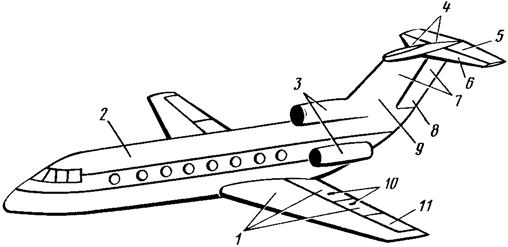
\includegraphics[width=0.5\linewidth]{img/parts-of-plane}
		\caption{Основные части самолета:\\\small{\textit{1} --- крыло; \textit{2} --- фюзеляж; \textit{3} --- силовая установка; \textit{4} --- горизонтальное оперение; \textit{5} --- руль высоты; \textit{6} --- стабилизатор; \textit{7} --- вертикальное оперение; \textit{8} --- руль направления; \textit{9} --- киль; \textit{10} --- закрылки; \textit{11} -- элерон.}}
		\label{fig:parts-of-plane}
	\end{figure}\par
	\textbf{Крыло} (рис.~\ref{fig:wing-about}), называемое иногда несущей поверхностью, представляет собой часть самолета, форма которой характеризуется тем, что один ее размер (толщина) значительно меньше других. Обычно крыло имеет плоскость симметрии. Крыло предназначено для создания подъемной силы, необходимой для уравновешивания силы тяжести самолета и искривления траектории полета.
	\begin{figure}[htbp]
		\centering
		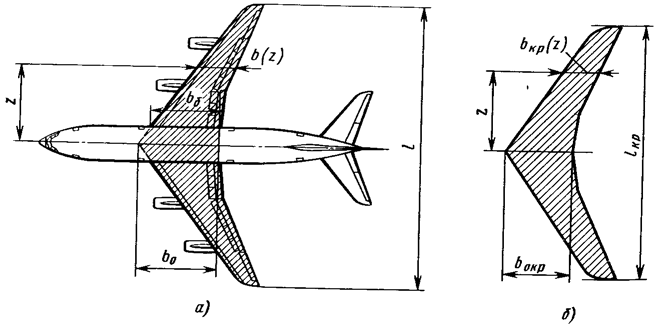
\includegraphics[width=0.6\linewidth]{img/wing-about}
		\caption{Крыло:\\\small{\textit{a} --- крыло с подфюзеляжной частью; \textit{б} --- крыло, составленное из консолей, $b_{0_\text{кр}}=b_0$.}}
		\label{fig:wing-about}
	\end{figure}\par
	Под \textbf{крылом с подфюзеляжной частью} понимают крыло, получаемое продолжением передних и задних кромок внутрь фюзеляжа.\par
	\textbf{Крылом, составленным из консолей}, называют крыло, составленное из находящихся в потоке частей крыла самолета, отделенных от фюзеляжа по бортовым сечениям.\par
	\textbf{Размах крыла} $l$ (как составленного из консолей, так и крыла с подфюзеляжной частью) --- расстояние между двумя плоскостями, параллельными базовой плоскости самолета (плоскости симметрии крыла) и касающимися концов крыла. На рис.~\ref{fig:wing-about} индексами «кр» обозначены параметры крыла, составленного из консолей.\par
	\textbf{Профиль крыла} --- местное сечение крыла плоскостью, параллельной базовой плоскости самолета.\par
	\textbf{Местная хорда крыла} $b\left(z\right)$ --- отрезок прямой, соединяющей наиболее удаленные точки профиля.\par
	\textbf{Центральная хорда крыла} $b_0$ --- хорда, ледащая в базовой плоскости самолета. Если рассматривается изолированное крыло, то центральная хорда лежит в плоскости его симметрии.\par
	\textbf{Базовая плоскость крыла} --- плоскость, содержащая центральную хорду и перпендикулярная базовой плоскости самолета. У изолированного крыла она перпендикулярна плоскости его симметрии.\par
	\begin{figure}[htbp]
		\centering
		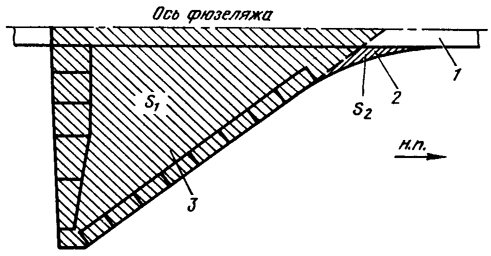
\includegraphics[width=0.5\linewidth]{img/wing-about-2}
		\caption{Определение площади крыла:\\\small{\textit{1} --- фюзеляж; \textit{2} --- наплыв; \textit{3} --- полукрыло.}}
		\label{fig:wing-about-2}
	\end{figure}\par
	\textbf{Площадь крыла} $S$ --- площадь проекции крыла на его базовую плоскость. При расчете аэродинамических характеристик самолета обычно характерной площадью считают площадь крыла с подфюзеляжной частью: $S=2S_1$ (рис.~\ref{fig:wing-about-2}). В некоторых случаях в площадь крыла включают площадь наплывов:
	\[ S = 2\left(S_1+S_2\right) \]\par
	\textbf{Средняя аэродинамическая хорда (СAX)} $b_\text{А}$ --- условная хорда.\par
	\textbf{Закрылки} применяют для увеличения подъемной силы самолета при сохранении его положения (сохранении угла атаки). Их отклоняют (выпускают) на взлете и посадке. Подъемная сила возрастает вследствие увеличения кривизны крыла.\par
	На рис.~\ref{fig:flaps-about} показан закрылок, состоящий из трех звеньев (трехщелевой закрылок) и имевший ранее широкое распространение щиток, применявшийся для тех же целей, что и закрылок.\par
	\textbf{Предкрылки} предназначены для предотвращения преждевременного отрыва потока от крыла. Это достигается за счет искривления крыла у передней кромки и выдува струи на верхнюю поверхность через щель.
	\begin{figure}[htbp]
		\centering
		\begin{minipage}{0.48\textwidth}
			\centering
			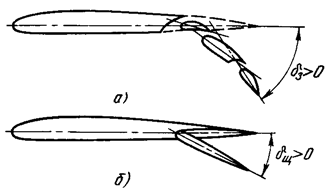
\includegraphics[width=\textwidth]{img/flaps-about}
			\captionof{figure}{Механизация задней кромки крыла:\\\small{\textit{а} --- закрылок; \textit{б} --- щиток.}}
			\label{fig:flaps-about}
		\end{minipage}
		\hfill
		\begin{minipage}{0.48\textwidth}
			\centering
			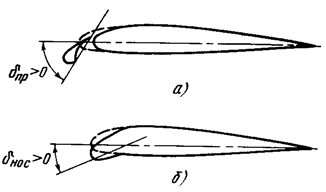
\includegraphics[width=\textwidth]{img/slats-about}
			\captionof{figure}{Механизация передней кромки крыла:\\\small{\textit{а} --- предкрылок; \textit{б} --- отклоняемый носок.}}
			\label{fig:slats-about}
		\end{minipage}
	\end{figure}\par
	Обычно закрылки и щитки называют \textit{механизацией задней кромки}, а предкрылки, отклоняемые носки и др., устанавливаемые на передней кромке устройства, --- \textit{механизацией передней кромки}.\par
	\textbf{Элероны} являются органами поперечного управления. Они обеспечивают кренение самолета, его вращение вокруг продольной оси. Элероны устанавливают симметрично на правой и левой половинах крыла. При отклонении ручки управления влево (поворота штурвала влево) правый элерон отклоняется вниз, а левый --- вверх. При этом подъемная сила на правом полукрыле увеличивается, а на левом --- уменьшается. В результате возникает аэродинамический момент, стремящийся накренить самолет влево. При отклонении ручки вправо возникает момент, кренящий самолет вправо.\par
	\begin{figure}[htbp]
		\centering
		\begin{minipage}{0.49\textwidth}
			\centering
			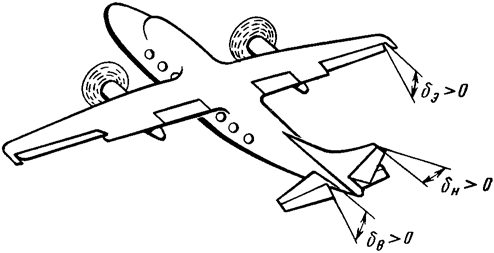
\includegraphics[width=\textwidth]{img/elerons-about}
			\captionof{figure}{Углы отклонения органов управления:\\\small{$\delta_\text{в}$ --- угол отклонения руля высоты; $\delta_\text{н}$ --- угол отклонения руля направления.}}
			\label{fig:elerons-about}
		\end{minipage}
		\hfill
		\begin{minipage}{0.49\textwidth}
			\centering
			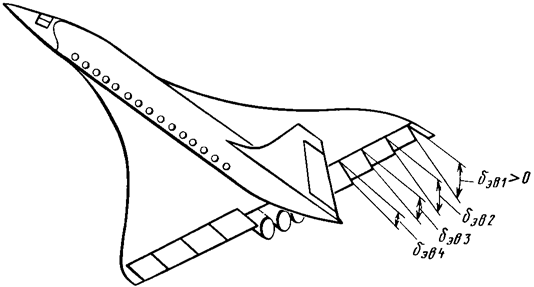
\includegraphics[width=\textwidth]{img/elevons-about}
			\captionof{figure}{Элевоны.}
			\label{fig:elevons-about}
		\end{minipage}
	\end{figure}\par
	На самолетах, не имеющих горизонтального оперения, (бесхвостках, летающих крыльях) вдоль задней кромки крыла устанавливают \textit{элевоны} (рис.~\ref{fig:elevons-about}), являющиеся органами продольного и поперечного управления. При отклонении элевонов на обеих половинах крыла вниз возникает момент, стремящийся опустить нос самолета. Если элевоны, расположенные на правом и левом полукрыльях, отклонить в разные стороны, то возникает соответствующий момент крена. Обычно элевоны разделяют на секции. В этом случае одни секции можно использовать как орган продольного управления, другие --- как орган поперечного управления, а третьи --- для управления как продольным, так и поперечным движением.\par
	\begin{figure}[htbp]
		\centering
		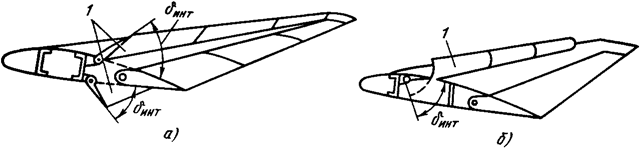
\includegraphics[width=1\linewidth]{img/interceptors-about}
		\caption{Интерцепторы:\\\small{\textit{а} --- поворотные; \textit{б} --- выдвижные; \textit{1} --- интерцептор.}}
		\label{fig:interceptors-about}
	\end{figure}
	\textbf{Интерцепторами} называют щитки, устанавливаемые на крыле. Их делают поворотными и выдвижными (рис.~\ref{fig:interceptors-about}) и располагают как на верхней, так и на нижней поверхностях крыла. Интерцепторы используют для управления креном (вместо элеронов).\par
	При отклонении интерцептора, установленного на верхней поверхности, давление перед ним увеличивается, а под крылом --- уменьшается. В результате возникает момент крена, стремящийся опустить консоль с отклоненным интерцептором. При отклонении интерцептора несколько возрастает разряжение за ним. Но это мало сказывается на значении момента крена. Установленные под крылом интерцепторы создают момент крена за счет увеличения подъемной силы на том полукрыле, на котором они отклонены (выдвинуты). Интерцепторы применяют также для уменьшения пробега при посадке и прерванном взлете.\par
	\textbf{Фюзеляж} предназначен для размещения экипажа, пассажиров, оборудования, топлива, грузов, силовой установки. Обычно он создает небольшую подъемную силу и значительное сопротивление.\par
	\textbf{Оперение} самолета состоит из горизонтального (ГО) и вертикального (ВО) оперений и предназначено для обеспечения устойчивости и управляемости. В зависимости от наличия и расположения ГО различают следующие схемы самолетов: нормальную (ГО позади крыла); «утку» (ГО впереди крыла), «бесхвостку» (ГО отсутствует). На дозвуковых самолетах горизонтальное оперение состоит обычно из стабилизатора и руля высоты, на сверхзвуковых --- только из управляемого стабилизатора, выполняющего функции как стабилизатора, так и руля высоты (ЦПГО).\par
	\textbf{Взлетно-посадочные устройства} включают в себя шасси, механизацию крыла, разгонные и тормозные устройства.\par
	\textbf{Силовая установка} состоит из авиационных двигателей с устройствами и системами, обеспечивающими их работу, воздухозаборников, воздушных винтов, сопел и т. д. Силовая установка предназначена для создания тяги и получения энергии, необходимой для работы систем самолета.\par
	\textbf{Системы управления} состоят из бортовых устройств, обеспечивающих управление движением самолета при полете и движении по земле.\par
	\textbf{Оборудование самолета} включает в себя пилотажно-навигационные приборы, навигационные системы, системы обеспечения жизнедеятельности экипажа, антиобледенительную систему и др. В зависимости от решаемой задачи и технических условий оно может быть различным.
	
	\subsection{Системы координат}
	При изучении аэродинамики самолетов и их частей чаще всего используют связанную $OXYZ$ и скоростную $O X_a Y_a Z_a$ системы координат. Обе системы являются правыми прямоугольными.\par
	\begin{figure}[htbp]
		\centering
		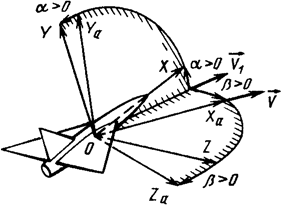
\includegraphics[width=0.5\linewidth]{img/coordinates-systems}
		\caption{Системы координат:\\\small{$OXYZ$ --- связанная система координат; $O X_a Y_a Z_a$ --- скоростная система координат; $\protect\vv{V}$ --- скорость самолета; $\protect\vv{V_1}$ --- проекция $\protect\vv{V}$ на базовую плоскость самолета; $\alpha$ --- угол атаки; $\beta$ --- угол скольжения.}}
		\label{fig:coordinates-systems}
	\end{figure}
	\textbf{Связанная система координат} обычно фиксирована относительно самолета и движется вместе с ним. Ее начало $O$ помещают в центре масс. Оси $OX,\;OY,\;OZ$ называют продольной, нормальной и поперечной осями. Оси $OX$ и $OY$ располагают в базовой плоскости самолета или в параллельной ей плоскости. Первую направляют от хвостовой части самолета к носовой, а вторую --- в сторону верхней части самолета. Ось $OZ$ проводят перпендикулярно базовой плоскости самолета и направляют к правой части самолета.\par
	В \textbf{скоростной системе координат} $O X_a Y_a Z_a$ начало также обычно помещают в центре масс. В этой системе различают скоростную ось $OX_a$, ось подъемной силы $OY_a$ и боковую ось $OZ_a$. Скоростную ось направляют вдоль вектора скорости самолета --- скорости начала $O$ связанной системы координат относительно среды, не возмущенной летательным аппаратом. Ось подъемной силы проводят в базовой плоскости самолета (или в параллельной ей плоскости, если начало $O$ находится вне базовой плоскости самолета) и направляют к верхней части самолета. Боковую ось $OZ_a$ проводят так, чтобы она дополнила оси $OX_a$, $OY_a$ до правой системы координат.\par
	Скоростная система не связана жестко с самолетом и может в полете менять свою ориентацию по отношению к нему.\par
	Угол между продольной осью $OX$ и проекцией вектора скорости самолета на плоскость $OXY$ связанной системы координат называют \textit{углом атаки} и обозначают $\alpha$. Угол атаки считают положительным, если проекция вектора скорости на нормальную ось отрицательна («если поднят нос»).\par
	Угол между вектором скорости и базовой плоскостью самолета обозначают $\beta$ и называют \textit{углом скольжения}. Он положителен, если проекция скорости на поперечную ось положительна (если выдвинута вперед правая консоль).\par
	\begin{figure}[htbp]
		\centering
		\begin{minipage}{0.49\textwidth}
			\centering
			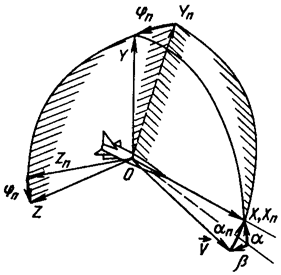
\includegraphics[width=0.8\textwidth]{img/linked-with-angle-system}
			\captionof{figure}{Связанная с пространственным углом атаки система координат.}
			\label{fig:linked-with-angle-system}
		\end{minipage}
		\hfill
		\begin{minipage}{0.49\textwidth}
			\centering
			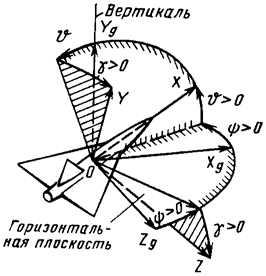
\includegraphics[width=0.8\textwidth]{img/normal-system}
			\captionof{figure}{Нормальная система координат.}
			\label{fig:normal-system}
		\end{minipage}
	\end{figure}\par
	При вращении летптельного аппарата целесообразно использовать \textbf{связанную с пространственным углом атаки} систему координат $OX_\text{п} Y_\text{п} Z_\text{п}$ (рис.~\ref{fig:linked-with-angle-system}). Ее ось $OX_\text{п}$ совпадает с продольной осью $OX$, ось $OY_\text{п}$ лежит в плоскости, образованной продольной осью $OX$ и вектором скорости $\protect\vv{V}$, и направлена противоположно проекции $\protect\vv{V}$ на плоскость $OYZ$. Ось $OZ_\text{п}$ дополняет систему до правой системы координат.\par
	Угол между осью $OX$ и вектором $\protect\vv{V}$ называют \textit{пространственным углом атаки} и обозначают $\alpha_\text{п}$. Пространственный угол атаки всегда положительный. Угол между осями $OY$ и $OY_\text{п}$ называют \textit{аэродинамическим углом крена} и обозначают $\varphi_\text{п}$. Он считается положительным, когда ось $OY_\text{п}$ совмещается с осью $OY$ поворотом вокруг продольной оси по часовой стрелке, если смотреть вдоль продольной оси.\par
	В некоторых случаях используют \textbf{нормальную систему координат} $OX_g Y_g Z_g$ (рис.~\ref{fig:normal-system}). Система подвижная правая. В ней начало $O$ совмещают с началом связанной системы координат. Ось $OY_g$, направляют вверх по местной вертикали, а направление осей $OX_g$ и $OY_g$ выбирают в соответствии с задачей. В этой системе плоскость $OX_g Z_g$ всегда расположена горизонтально.\par
	Угол между осью $OX_g$, и проекцией продольной оси на горизонтальную плоскость называют \textit{углом рыскания} и обозначают $\psi$ (см. рис.~\ref{fig:normal-system}). $\psi>0$, если ось $OX_g$ совмещается с проекцией продольной оси на горизонтальную плоскость поворотом вокруг оси $OY_g$ по часовой стрелке (если смотреть вдоль оси $OY_g$).\par
	Угол между продольной осью самолета $OX$ и горизонтальной плоскостью $OX_g Z_g$ называют \textit{углом тангажа} и обозначают $\vartheta$. Он положителен, если нос самолета поднят по отношению к его хвостовой части.\par
	Угол между поперечной осью $OZ$ и осью $OZ_g$ нормальной системы координат, смещенной в положение, при котором угол рыскания равен нулю, называют углом крена и обозначают $\gamma$. Угол между нормальной осью $OY$ и местной вертикальной плоскостью, содержащей продольную ось самолета $OX$, также равен $\gamma$. Угол $\gamma$ положителен, если опущена правая консоль. На рис.~\ref{fig:normal-system} углы $\psi$, $\vartheta$, $\gamma$ --- положительные.
	
	\subsection{Аэродинамические силы и моменты. Коэффициенты аэродинамических сил и моментов}
	\textit{Аэродинамическая сила планера} $\protect\vv{R_\text{А}}$ --- главный вектор системы сил, действующих на ЛА со стороны окружающей среды при его движении.\par
	\begin{figure}[htbp]
		\centering
		\begin{minipage}{0.49\textwidth}
			\centering
			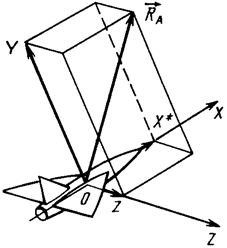
\includegraphics[width=0.75\textwidth]{img/Ra-in-linked-system}
			\captionof{figure}{Составляющие аэродинамической силы в связанной системе координат.}
			\label{fig:Ra-in-linked-system}
		\end{minipage}
		\hfill
		\begin{minipage}{0.49\textwidth}
			\centering
			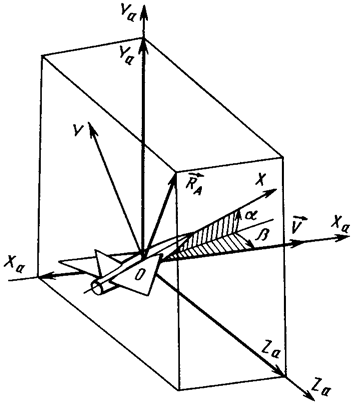
\includegraphics[width=0.75\textwidth]{img/Ra-in-speed-system}
			\captionof{figure}{Составляющие аэродинамической силы в скоростной системе координат.}
			\label{fig:Ra-in-speed-system}
		\end{minipage}
	\end{figure}\par
	Проектируя $\protect\vv{R_\text{А}}$ на оси связанной системы координат находят ее составляющие $X^*,\;Y,\;Z$ вдоль этих осей. Взятую с обратным знаком $X^*$ называют аэродинамической продольной силой и обозначают $X$. Отрицательная продольная сила действует в сторону носовой части самолета, а положительная --- в сторону кормы. На рис.~\ref{fig:Ra-in-linked-system} $X^*>0$, поэтому в данном случае продольная сила $X=X^*<0$ и направлена в сторону носовой части самолета. Составляющие аэродинамической силы $Y$, $Z$ называют \textit{аэродинамической нормальной} и \textit{аэродинамической поперечной силами}.\par
	Проекции $\protect\vv{R_\text{А}}$ на оси скоростной системы координат --- $X^{*}_a,\;Y_a,\;Z_a$. \textit{Сила лобового сопротивления} --- взятая с обратным знаком $X^{*}_a$, обозначается $X_a$. Составляющие $Y_a$ и $Z_a$ называют \textit{аэродинамической подъемной} и \textit{аэродинамической боковой силами}.\par
	Разделив значения аэродинамических сил на скоростной напор $q_\infty=\frac{\rho_\infty V^2_\infty}{2}$, где $\rho$ --- плотность невозмущенного воздуха; $V_\infty$ --- скорость невозмущенного потока, набегающего на самолет в обращенном движении, и на характерную площадь $S$ (площадь крыла с подфюзеляжной частью в случае самолета, площадь крыла или площадь горизонтального оперения при рассмотрении этих частей, площадь миделевого сечения в случае фюзеляжа, гондол и т. п.), находим коэффициенты аэродинамических сил:
	\begin{gather}
		\begin{gathered}
			c_x = \frac{X}{q_\infty S};\quad c_y = \frac{Y}{q_\infty S};\quad c_z = \frac{Z}{q_\infty S};\\
			c_{xa} = \frac{X_a}{q_\infty S};\quad c_{ya} = \frac{Y_a}{q_\infty S};\quad c_{za} = \frac{Z_a}{q_\infty S},
		\end{gathered}
	\end{gather}
	где $c_x,\;c_y,\;c_z,\;c_{ya},\;c_{za}$ --- коэффициенты продольной, нормальной, поперечной, подъемной и боковой сил, а $c_{xa}$ --- коэффициент лобового сопротивления.\par
	Главный вектор системы сил, действующих на летательный аппарат со стороны движетеля в результате его функционирования, называют тягой и обозначают $\protect\vv{P}$. Составляющие $\protect\vv{P}$ вдоль осей связанной и скоростной систем координат обозначают $P_x,\; P_y,\; P_z,\; P_{xa},\; P_{ya},\; P_{za}$. Разделив силы на $q_\infty$ и характерную площадь $S$, находим коэффициенты тяги:
	\begin{gather}
		\begin{gathered}
			c_P = \frac{P}{q_\infty S};\quad c_{P_x} = \frac{P_x}{q_\infty S};\quad c_{P_y} = \frac{P_y}{q_\infty S};\quad
			c_{P_z} = \frac{P_z}{q_\infty S};\\ c_{P_{xa}} = \frac{P_{xa}}{q_\infty S};\quad c_{P_{ya}} = \frac{P_{ya}}{q_\infty S};\quad c_{P_{za}} = \frac{P_{za}}{q_\infty S}.
		\end{gathered}
	\end{gather}\par
	Главный вектор системы сил, действующий на ЛА, без учета инерционных и гравитационных сил и сил, возникающих при контакте с землей, называют \textit{результирующей силой} и обозначают $\protect\vv{R}$. Имеем:
	\begin{gather}
		\vv{R} = \vv{R_\text{A}} + \vv{P}.
	\end{gather}\par
	При этом, $\protect\vv{R_\text{A}}$ определяют с учетом влияния работы двигателя, а $\protect\vv{P}$ --- с учетом влияния обтекания самолета.\par
	Составляющие результирующей силы по осям связанной системы координат обозначают $R_x,\; R_y,\; R_z$ и называют \textit{продольной}, \textit{нормальной} и \textit{поперечной силами}. А составляющие той же силы по осям скоростной системы координат обозначают $R_{xa},\; R_{ya},\; R_{za}$ и называют \textit{тангенциальной}, \textit{подъемной} и \textit{боковой силами}. Положительная продольная сила $R_x$ направлена в сторону носовой части самолета, а положительная аэродинамическая продольная сила $X$ --- в противоположную сторону. Аналогично соотносятся $R_{xa}$ и сила лобового сопротивления $X_a$: положительная тангенциальная сила направлена вдоль вектора скорости самолета, а сила лобового сопротивления --- в противоположную сторону.\par
	Разделив результирующую силу и ее составляющие на $q_\infty S$, находим коэффициенты этих сил:
	\begin{gather}
		\begin{gathered}
			c_R = \frac{R}{q_\infty S};\quad c_{R_x} = \frac{R_x}{q_\infty S};\quad c_{R_y} = \frac{R_y}{q_\infty S};\quad
			c_{R_z} = \frac{R_z}{q_\infty S};\\ c_{R_a} = \frac{R_a}{q_\infty S};\quad c_{R_{xa}} = \frac{R_{xa}}{q_\infty S};\quad c_{R_{ya}} = \frac{R_{ya}}{q_\infty S};\quad c_{R_{za}} = \frac{R_{za}}{q_\infty S}.
		\end{gathered}
	\end{gather}\par
	\begin{figure}[htbp]
		\centering
		\begin{minipage}{0.49\textwidth}
			\centering
			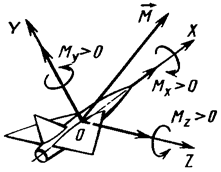
\includegraphics[width=0.5\textwidth]{img/aerodynamic-moment-parts}
			\captionof{figure}{Составляющие аэродинамического момента.}
			\label{fig:aerodynamic-moment-parts}
		\end{minipage}
		\hfill
		\begin{minipage}{0.49\textwidth}
			\centering
			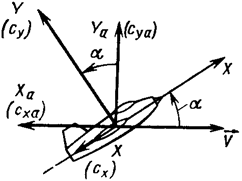
\includegraphics[width=0.5\textwidth]{img/aerodynamic-coefficients-in-systems}
			\captionof{figure}{Аэродинамические коэффициенты в связанной и скоростной системах координат.}
			\label{fig:aerodynamic-coefficients-in-systems}
		\end{minipage}
	\end{figure}\par
	Примем начало координат связанной системы $O$ (обычно это центр масс) за центр приведения аэродинамических сил, действующих на самолет. Момент, создаваемый этими силами, называют \textit{аэродинамическим моментом} и обозначают $\protect\vv{M}$. Составляющие $\protect\vv{M}$ вдоль осей связанной системы координат обозначают $M_x,\; X_y,\; M_z$ и называют \textit{аэродинамическими моментами крена}, \textit{рыскания} и \textit{тангажа} (рис.~\ref{fig:aerodynamic-moment-parts}). Положительные моменты стремятся повернуть самолет вокруг соответствующей оси по часовой стрелке, если смотреть в положительном направлении оси.\par
	Вводят коэффициенты моментов:
	\begin{gather}
		m_x = \frac{M_x}{q_\infty Sl};\quad m_y = \frac{M_y}{q_\infty Sl};\quad m_z = \frac{M_z}{q_\infty Sb},
	\end{gather}
	где $l$ --- размах крыла с подфюзеляжной частью; $b$ --- хорда крыла (обычно длина САХ крыла с подфюзеляжной частью). Коэффициенты $m_x,\; m_y,\; m_z$ называют \textit{коэффициентами аэродинамических моментов крена}, \textit{рыскания} и \textit{тангажа}.\par
	Момент тяги относительно центра приведения сил и его составляющие по осям связанной системы координат обозначают $\vv{M_P},\; M_{P_x},\; M_{P_y},\; M_{P_z}$. Коэффициенты моментов тяги определяют следующими соотношениями:
	\begin{gather}
		m_{P_x} = \frac{M_{P_x}}{q_\infty Sl};\quad m_{P_y} = \frac{M_{P_y}}{q_\infty Sl};\quad m_{P_z} = \frac{M_{P_z}}{q_\infty Sb}.
	\end{gather}\par
	Сложив аэродинамический момент с моментом тяги, получим \textit{результирующий момент}:
	\begin{gather}
		\vv{M_R} = \vv{M} + \vv{M_P}.
	\end{gather}\par
	Составляющие результирующего момента по осям связанной системы координат обозначают $M_{R_x},\; M_{R_y},\; M_{R_z},\;$ и называют \textit{моментами крена}, \textit{рыскания} и \textit{тангажа}. Коэффициенты этих моментов определяются выражениями:
	\begin{gather}
		m_{R_x} = \frac{M_{R_x}}{q_\infty Sl};\quad m_{R_y} = \frac{M_{R_y}}{q_\infty Sl};\quad m_{R_z} = \frac{M_{R_z}}{q_\infty Sb}.
	\end{gather}
	Очевидно, что:
	\begin{gather}
		m_{R_x} = m_x + m_{P_x};\quad m_{R_y} = m_y + m_{P_y};\quad m_{R_z} = m_z + m_{P_z}.
	\end{gather}\par
	До сих пор мы говорили о суммарных силах и моментах. Но в ряде случаев надо знать и местные силы, действующие на единичную площадь поверхности самолета в данной точке, т. е. напряжения местных сил. Такими напряжениями являются действующие по нормалям к поверхности давление $p$ и напряжение $\tau$, направленные по касательной к поверхности силы трения.\par
	Соответствующие безразмерные величины
	\begin{gather}
		c_p = \frac{p - p_\infty}{q_\infty}\quad \text{и} \quad c_f = \frac{\tau}{q_\infty}
	\end{gather}
	называют коэффициентом давления и местным коэффициентом трения.\par
	Приведем также формулы, определяющие соотношения между коэффициентами аэродинамических сил в связанной и скоростной системах координат, когда скольжения нет и обтекание симметричное. Из рис.~\ref{fig:aerodynamic-coefficients-in-systems} находим
	\begin{gather}
		c_{ya} = c_y\cos{\alpha} - c_x\sin{\alpha};\quad c_{xa} = c_x\cos{\alpha} + c_y\sin{\alpha},\label{eq:120}\\
		c_{y} = c_{ya}\cos{\alpha} + c_{xa}\sin{\alpha};\quad c_{x} = c_{xa}\cos{\alpha} - c_{ya}\sin{\alpha}.\label{eq:121}
	\end{gather}\par
	При малых $\alpha \; \sin{\alpha} \cong \alpha;\; \cos{\alpha} \cong 1; \; c_y,\;c_{ya}$ --- малые того же порядка, что и $\alpha$, а $c_x,\; c_{ya}$ --- величины второго порядка малости. Учитывая это, из \eqref{eq:120}, \eqref{eq:121} получаем следующие формулы, справедливые при малых $\alpha$:
	\begin{gather}
		c_{ya} = c_y; \quad c_{xa} = c_x + c_y\alpha.
	\end{gather}
	
	\newpage
	\part{Кинематика жидкости (газа)}
	
	\section{Лекция 2}
	
	\subsection{Методы кинематического исследования движения жидкости (газа)}
	Задача кинематического анализа движения жидкости заключается в определении значений скорости в каждой точке движущейся жидкости для любого момента времени $t$. Зная значения скоростей, можно, как показано ниже, найти распределение давления, а следовательно, и силы, действующие в жидкости. Движение жидкости можно изучать методами Эйлера и Лагранжа.\par
	
	\subsubsection{Метод Эйлера}
	В \textit{методе Эйлера} фиксируется точка пространства с координатами $x,\;y,\;z$ и исследуется изменение скорости в этой точке с течением времени. Совокупность величин $x,\;y,\;z,\;t$ называют \textit{переменными Эйлера}. Следовательно, движение жидкости по методу Эйлера задается следующим образом:
	\begin{gather}
		v_x = f_1(x,\;y,\;z,\;t);\quad v_y = f_2(x,\;y,\;z,\;t);\quad v_z = f_3(x,\;y,\;z,\;t).
	\end{gather}\par
	Предполагая движение жидкости непрерывным, будем считать. указанные функции однозначными, непрерывными и дифференцируемыми функциями координат $x,\;y,\;z$ и времени $t$.\par
	Проекции ускорения жидких частиц в переменных Эйлера:
	\[ w_x = \frac{\dd v_x}{\dd t},\quad w_y = \frac{\dd v_y}{\dd t},\quad w_z = \frac{\dd v_z}{\dd t}. \]\n
	Используя правило дифференцирования сложной функции, получаем
	\[ \frac{\mathrm{d}v_x}{\mathrm{d}t} = \frac{\partial v_x}{\partial t} + \frac{\pp v_x}{\pp x}\frac{\dd x}{\dd t} + \frac{\pp v_x}{\pp y}\frac{\dd y}{\dd t} + \frac{\pp v_x}{\pp z}\frac{\dd z}{\dd t}, \]
	или так как $\dfrac{\dd x}{\dd t}=v_x,\; \dfrac{\dd y}{\dd t}=v_y,\; \dfrac{\dd z}{\dd t}=v_z,$ то
	\begin{gather}
		\frac{\dd v_x}{\dd t} = \frac{\pp v_x}{\pp t} + v_x\frac{\pp v_x}{\pp x} + v_y\frac{\pp v_x}{\pp y} + v_z\frac{\pp v_x}{\pp z}.\label{eq:22}
	\end{gather}\n
	Аналогично,
	\begin{gather}
		\begin{dcases}\label{eq:23}
			\frac{\dd v_y}{\dd t} = \frac{\pp v_y}{\pp t} + v_x\frac{\pp v_y}{\pp x} + v_y\frac{\pp v_y}{\pp y} + v_z\frac{\pp v_y}{\pp z};\\
			\frac{\dd v_z}{\dd t} = \frac{\pp v_z}{\pp t} + v_x\frac{\pp v_z}{\pp x} + v_y\frac{\pp v_z}{\pp y} + v_z\frac{\pp v_z}{\pp z}.
		\end{dcases}
	\end{gather}\n
	Следует отметить, что когда берутся полные производные \eqref{eq:22} и \eqref{eq:23}, то учитывается не только изменение составляющих скорости по времени $t$, но и их изменение в зависимости от координат частицы жидкости $x,\; y,\; z$. Эти производные называются \textit{конвективными}. Частные производные по времени берутся, как обычно, при фиксированных значениях координат $x,\; y,\; z$ и называются \textit{локальными производными}.\n
	
	\subsubsection{Метод Лагранжа}
	Второй путь изучения движения жидкости, называемый \textit{методом Лагранжа}, в отличие от метода Эйлера, рассматривает движение индивидуальных частиц вдоль их траектории. Так как жидких частиц бесчисленное множество, то данную частицу следует как-то характеризовать. Это можно сделать, если в качестве характеристики жидкой частицы выбрать ее координаты в начальный момент времени $t = 0$. Пусть при $t = 0$ координаты частицы будут $a,\; b,\; c$. Это означает, что из всей бесчисленной совокупности траекторий частице принадлежит та, которая проходит через точку $a,\; b,\; c$. Таким образом, координаты рассматриваемой жидкой частицы $x,\;y,\;z$ зависят от величин $a,\; b,\; c,\; t$ называемых \textit{переменными Лагранжа}, т. е.
	\begin{gather}
		x = \varphi_1(a,\; b,\; c,\; t); \quad y = \varphi_2(a,\; b,\; c,\; t); \quad z = \varphi_3(a,\; b,\; c,\; t).\label{eq:24}
	\end{gather}\n
	Выражения \eqref{eq:24} представляют собой уравнения семейства траекторий, заполняющих все пространство, занятое жидкостью; величины а, b, с являются параметрами, определяющими траекторию. Пользуясь этими уравнениями, находим проекции скорости и ускорения частиц:
	\begin{gather}
		\begin{dcases}
			v_x = \frac{\pp x}{\pp t},\quad v_y = \frac{\pp y}{\pp t},\quad v_z = \frac{\pp z}{\pp t};\\
			w_x = \frac{\pp^2 x}{\pp t^2},\quad w_y = \frac{\pp^2 y}{\pp t^2},\quad w_z = \frac{\pp^2 z}{\pp t^2}.
		\end{dcases}
	\end{gather}\n
	Метод Эйлера получил преимущественное применение в аэродинамике, так как он более прост и дает возможность широко использовать хорошо развитый раздел математики --- векторный анализ.
	
	\subsubsection{Классификация движений жидкости (газа)}\label{sec:fluid-moving-classification}
	Проекции скорости $v_x,\; v_y,\; v_z$ в наиболее общем случае \textit{неустановившегося} движения жидкости (газа) являются функциями координат $x,\; y,\; z$ и времени $t$:
	\begin{gather}
		v_x = f_1(x,\;y,\;z,\;t);\quad v_y = f_2(x,\;y,\;z,\;t);\quad v_z = f_3(x,\;y,\;z,\;t).
	\end{gather}\n
	Если в фиксированной точке пространства величины $v_x,\; v_y,\; v_z$ со временем не изменяются, то движение называют \textit{установившимся}. В этом случае
	\begin{gather}
		v_x = f_1(x,\; y,\; z);\quad v_y = f_2(x,\;y,\;z);\quad v_z = f_3(x,\;y,\;z).
	\end{gather}\n
	Движение жидкости (газа) называется \textit{плоскопараллельным}, если все частицы, находящиеся на одном и том же перпендикуляре к некоторой фиксированной плоскости, движутся параллельно этой плоскости с одинаковыми скоростями. В плоскопараллельном $\left(v_z=0\right)$ неустановившемся потоке $v_x = f_1(x,\; y,\; t),\; v_y = f_2(x,\; y,\; t)$, а в установившемся потоке $v_x = f_1(x,\; y),\; v_y = f_2(x,\; y)$.\n
	Течение называют \textit{осесимметричным}, если оно симметрично относительно некоторой оси, т. е. одинаково во всех плоскостях, проходящих через ось симметрии. Такие плоскости называются \textit{меридиональными}. Примеры --- течение в диффузорах и соплах круглого сечения, течение при обтекании тела вращения потоком, направленным вдоль его оси.\n
	Течение называют \textit{коническим}, если при обтекании тела потоком скорость сохраняет постоянное значение вдоль прямых, проведенных из некоторой фиксированной точки --- полюса конического течения. Например, обтекание конуса под углом атаки.
	
	\subsection{Линия тока}
	\begin{figure}[H]
		\centering
		\begin{minipage}{0.49\textwidth}
			\centering
			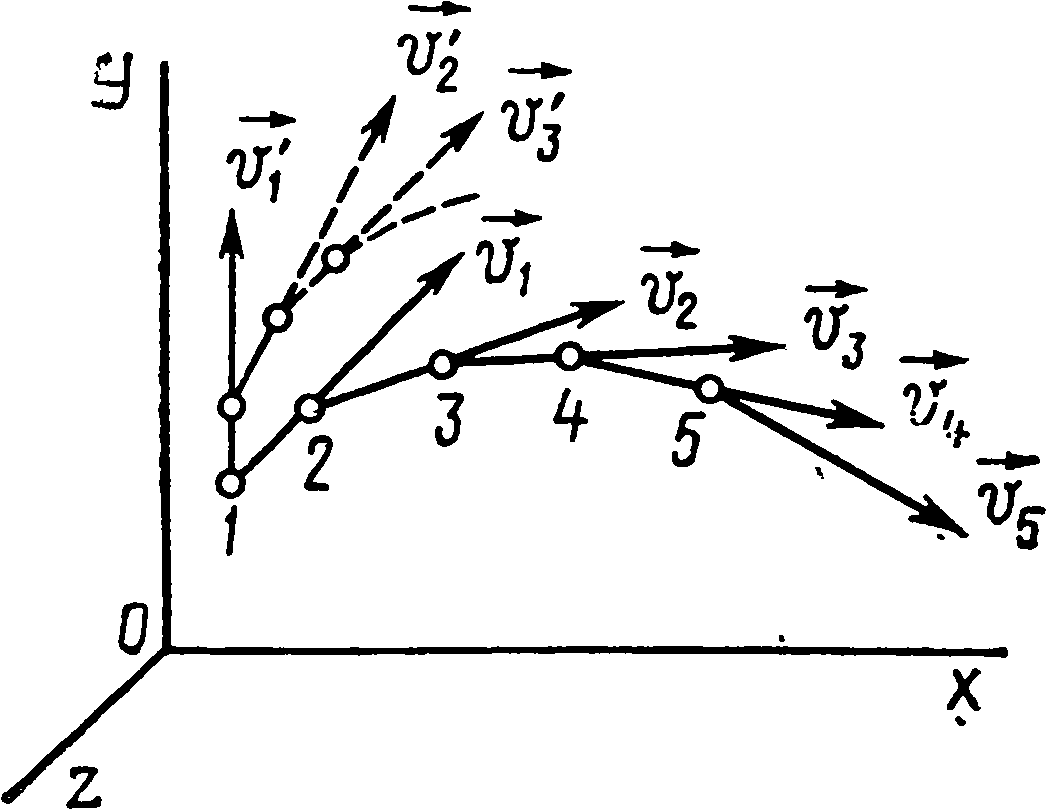
\includegraphics[width=0.5\textwidth]{img/flow-line-plot}
			\captionof{figure}{Построение линии тока.}
			\label{fig:flow-line-plot}
		\end{minipage}
		\hfill
		\begin{minipage}{0.49\textwidth}
			\centering
			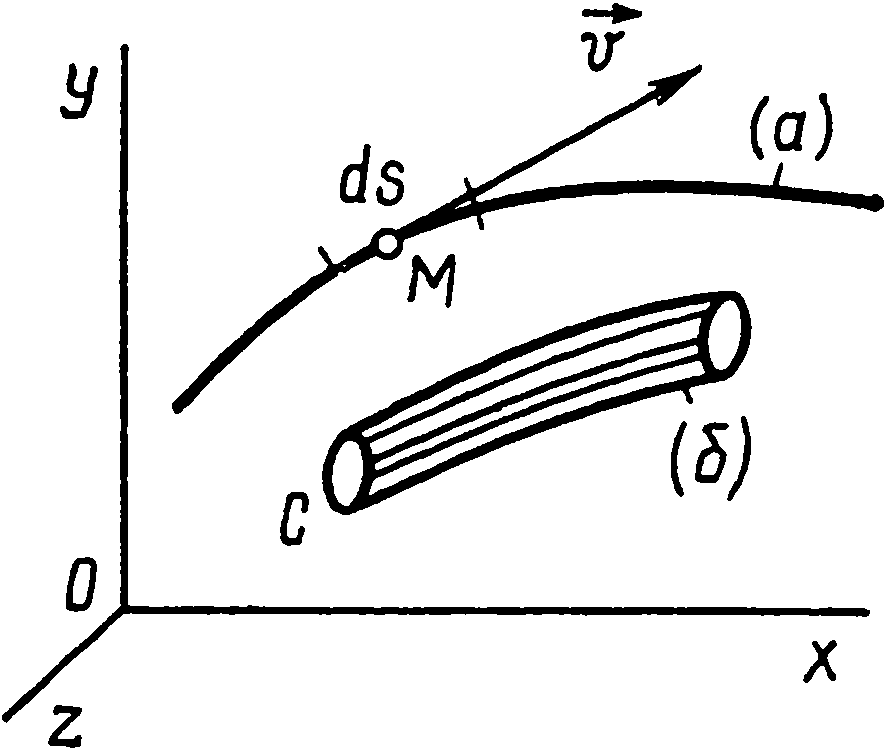
\includegraphics[width=0.5\textwidth]{img/flow-line-and-flow-tube}
			\captionof{figure}{Линия тока (\textit{а}) и трубка тока (\textit{б}).}
			\label{fig:flow-line-and-flow-tube}
		\end{minipage}
	\end{figure}
	Рассмотрим в момент времени $t$ какую-либо точку пространства, заполненного жидкостью. Пусть скорость находящейся в ней частицы жидкости изображается вектором $\vv{v_1}$ (рис.~\ref{fig:flow-line-plot}). В этот же момент времени $t$ возьмем на векторе скорости $\vv{v_1}$ точку \textit{2}, бесконечно близкую к точке \textit{1}. В этой точке находится другая частица жидкости. Так как точка 2 имеет другие координаты, чем точка 1, то и скорость в ней другая, изображаемая вектором $\vv{v_2}$. В тот же момент времени $t$ возьмем на векторе скорости $\vv{v_2}$ точку \textit{3}, бесконечно близкую к точке \textit{2}. В ней вектор скорости $\vv{v_3}$ и т. д. В результате такого построения (в данный момент времени) получается ломаная \textit{1-2-3-4-5-\dots}, обладающая тем свойством, что вектор скорости, соответствующий начальной точке любого ее звена, направлен вдоль этого звена.\n
	Будем неограниченно увеличивать число звеньев ломаной, устремляя к нулю длину каждого ее звена. Тогда в пределе (рис.~\ref{fig:flow-line-and-flow-tube}) получится кривая, называемая \textit{линией тока}. Следовательно, линия тока обладает тем свойством, что \textit{каждая частица жидкости (газа), находящаяся на ней в данный момент времени, имеет скорость, совпадающую по направлению с касательной к этой линии}.\n
	Рассмотрим распределение скоростей  в момент времени $t'$. Если движение неустановившееся, то в момент времени $t'$ в точке \textit{1} скорость $\vv{v'_1}$ отлична от вектора $\vv{v_1}$. Следовательно, для того чтобы передвинуться в соседнюю бесконечно близкую точку, нужно двигаться по новому направлению, изображенному на рис.~\ref{fig:flow-line-plot} пунктиром. Отсюда следует, что для момента $t'$ линия тока иная. Это означает, что при \textit{неустановившемся движении совокупность линий тока изменяется по времени}.\n
	Если же движение установившееся, т. е. скорости в точках \textit{1}, \textit{2} и других не изменяются по времени, то очевидно, что и линии тока не изменяются с течением времени. В случае установившегося движения линии тока и траектории совпадают.\n
	Составим дифференциальное уравнение линий тока. Из условия совпадения в данной точке линии тока вектора скорости $\vv{v}\left(v_x,\; v_y,\; v_z\right)$ с касательной к этой линии $\vv{\dd s}\left(\dd x,\; \dd y,\; \dd z\right)$ следует, что
	\begin{gather}
		\frac{\dd x}{v_x(x,\; y,\; z,\; t)} = \frac{\dd y}{v_y(x,\; y,\; z,\; t)} = \frac{\dd z}{v_z(x,\; y,\; z,\; t)}.\label{eq:28}
	\end{gather}\n
	Выражение \eqref{eq:28} представляет собой \textit{дифференциальное уравнение линий тока}.\n
	Введем понятие о трубке тока. Для этого проведем в жидкости некоторый малый замкнутый контур \textit{С}, не являющийся линией тока, и через каждую точку этого контура проведем линию тока. Совокупность проведенных таким образом линий тока образует поверхность, называемую \textit{трубкой тока}. Жидкость, протекающую внутри трубки тока, принято называть \textit{струйкой}.
	
	\subsection{Циркуляция скорости}
	\begin{figure}[H]
		\centering
		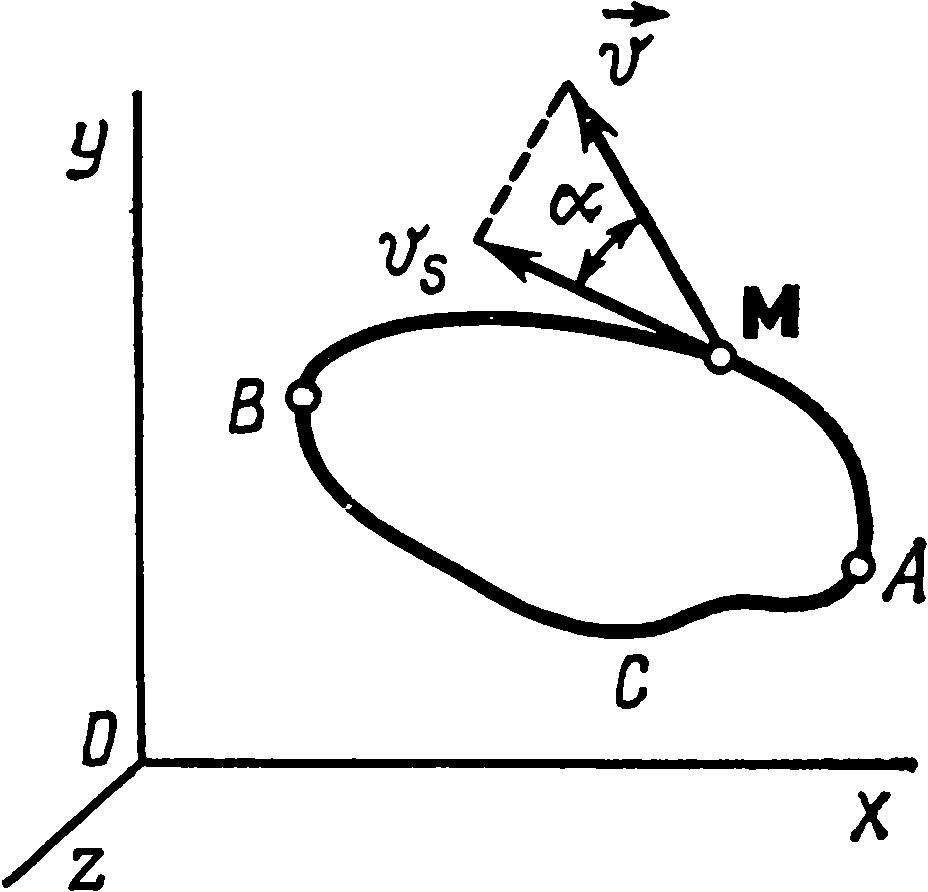
\includegraphics[width=0.25\linewidth]{img/velocity-circulation-definition}
		\caption{Определение циркуляции скорости.}
		\label{fig:velocity-circulation-definition}
	\end{figure}
	Выделим в движущейся жидкости произвольный фиксированный в пространстве замкнутый контур \textit{C} (рис.~\ref{fig:velocity-circulation-definition}). Пусть в некоторой его точке \textit{M} скорость изображается вектором $\vv{v}$. Составим произведение $v_s \dd s$, где $v_s$ --- проекция вектора скорости на направление касательной к контуру в точке \textit{M}. Возьмем от этого выражения криволинейный интеграл по дуге \textit{AB}. Тогда
	\begin{gather}
		\Gamma = \int\limits_{AB} v_s \dd s.
	\end{gather}\n
	Это выражение называется \textit{циркуляцией скорости} по дуге \textit{AB}. Обычно циркуляцию $\Gamma$ определяют по всему замкнутому контуру \textit{C}:
	\begin{gather}
		\Gamma = \oint\limits_{C} v_s \dd s.\label{eq:210}
	\end{gather}\n
	Направление обхода контура \textit{C} будем считать положительным, если охватываемая контуром \textit{C} область остается при этом слева. Заменяя в выражении \eqref{eq:210} $v_s$ на $v \cos\alpha$, получаем
	\begin{gather}
		\Gamma = \oint\limits_{C} v \cos\alpha\; \dd s.\label{eq:211}
	\end{gather}\n
	Замечая, что подынтегральное выражение в формуле \eqref{eq:211} является скалярным произведением векторов $\vv{v}$ и $\vv{\dd s}$, циркуляцию представим в следующем виде:
	\begin{gather}
		\Gamma = \oint\limits_{C} v_x\dd x + v_y\dd y + v_z\dd z,
	\end{gather}
	где $v_x,\; v_y,\; v_z$ --- составляющие скорости потока.
	
	\subsection{Движение жидкой частицы}
	
	\subsubsection{Вывод выражений для проекций скоростей}
	\begin{figure}[htbp]
		\centering
		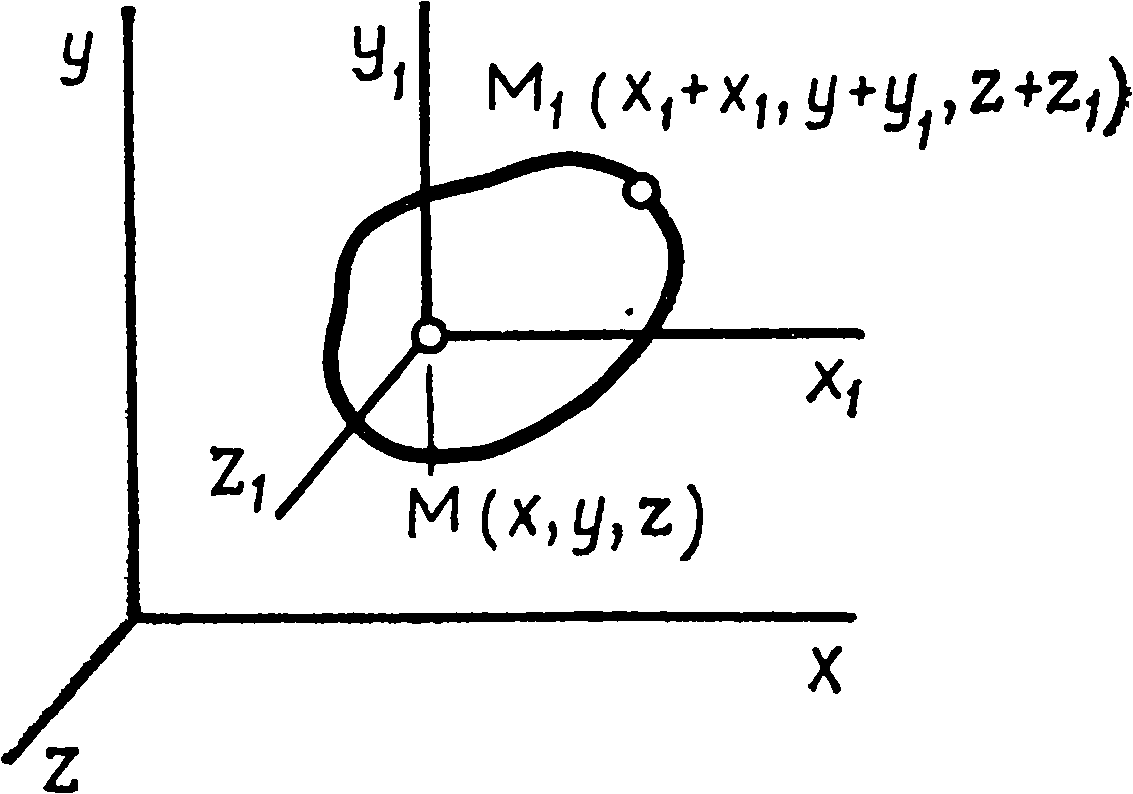
\includegraphics[width=0.3\linewidth]{img/part-of-fluid-moving}
		\caption{Движение частицы жидкости.}
		\label{fig:part-of-fluid-moving}
	\end{figure}
	Рассмотрим в какой-либо момент времени $t$ движение бесконечно малой жидкой частицы. Пусть в некоторой точке $M(x,\; y,\; z)$ внутри частицы (рис.~\ref{fig:part-of-fluid-moving}) проекции скорости $v_x(x,\; y,\; z),\; v_y(x,\; y,\; z),\; v_z(x,\; y,\; z)$. Тогда проекция скорости в некоторой точке $M_1(x+x_1,\; y+y_1,\; z+z_1)$ на поверхности частицы можно представить в виде
	\begin{gather*}
		\begin{gathered}
			v_{x_1} = v_x(x+x_1,\; y+y_1,\; z+z_1);\\
			v_{y_1} = v_y(x+x_1,\; y+y_1,\; z+z_1);\\
			v_{z_1} = v_z(x+x_1,\; y+y_1,\; z+z_1).
		\end{gathered}
	\end{gather*}\n
	Воспользовавшись разложением в ряд Тейлора и удерживая в нем только величины первого порядка малости, т. е. члены, содержащие $x_1,\; y_1,\; z_1$ в степени не выше первой, получим следующее выражение для скоростей:
	\begin{gather}
		\begin{dcases}\label{eq:213}
			v_{x_1} = v_x + \frac{\pp v_x}{\pp x}x_1 + \frac{\pp v_x}{\pp y}y_1 + \frac{\pp v_x}{\pp z}z_1;\\
			v_{y_1} = v_y + \frac{\pp v_y}{\pp x}x_1 + \frac{\pp v_y}{\pp y}y_1 + \frac{\pp v_y}{\pp z}z_1;\\
			v_{z_1} = v_z + \frac{\pp v_z}{\pp x}x_1 + \frac{\pp v_z}{\pp y}y_1 + \frac{\pp v_z}{\pp z}z_1,
		\end{dcases}
	\end{gather}
	где для краткости положено $v_x = v_x(x,\; y,\; z),\; v_y = v_y(x,\; y,\; z),\; v_z = v_z(x,\; y,\; z)$.\n
	Прибавим к правой части первого уравнения \eqref{eq:213} величины $\pm\dfrac{1}{2}\dfrac{\pp v_y}{\pp x}y_1$ и $\pm\dfrac{1}{2}\dfrac{\pp v_z}{\pp x}z_1$ и перегруппируем члены. В результате имеем
	\begin{align*}
		v_{x_1} = v_x + \frac{\pp v_x}{\pp x}x_1 &+ \frac{1}{2}\left(\frac{\pp v_x}{\pp y} + \frac{\pp v_y}{\pp x}\right)y_1 + \frac{1}{2}\left(\frac{\pp v_x}{\pp z} + \frac{\pp v_z}{\pp x}\right)z_1 +\\&+ \frac{1}{2}\left(\frac{\pp v_x}{\pp z} - \frac{\pp v_z}{\pp x}\right)z_1 - \frac{1}{2}\left(\frac{\pp v_y}{\pp x} - \frac{\pp v_x}{\pp y}\right)y_1.
	\end{align*}\n
	Аналогичными преобразованиями из второго и третьего уравнений \eqref{eq:213} можно получить:
	\begin{gather*}
		\begin{aligned}
			v_{y_1} = v_y + \frac{\pp v_y}{\pp y}y_1 &+ \frac{1}{2}\left(\frac{\pp v_y}{\pp x} + \frac{\pp v_x}{\pp y}\right)x_1 + \frac{1}{2}\left(\frac{\pp v_z}{\pp y} + \frac{\pp v_y}{\pp z}\right)z_1 +\\&+ \frac{1}{2}\left(\frac{\pp v_y}{\pp x} - \frac{\pp v_x}{\pp y}\right)x_1 - \frac{1}{2}\left(\frac{\pp v_z}{\pp y} - \frac{\pp v_y}{\pp z}\right)z_1;
		\end{aligned}\\
		\begin{aligned}
			v_{z_1} = v_z + \frac{\pp v_z}{\pp z}z_1 &+ \frac{1}{2}\left(\frac{\pp v_x}{\pp z} + \frac{\pp v_z}{\pp x}\right)x_1 + \frac{1}{2}\left(\frac{\pp v_z}{\pp y} + \frac{\pp v_y}{\pp z}\right)y_1 +\\&+ \frac{1}{2}\left(\frac{\pp v_z}{\pp y} - \frac{\pp v_y}{\pp z}\right)y_1 - \frac{1}{2}\left(\frac{\pp v_x}{\pp z} - \frac{\pp v_z}{\pp x}\right)x_1.
		\end{aligned}
	\end{gather*}\n
	Введем обозначения:
	\begin{gather}
		\omega_x = \frac{1}{2}\left(\frac{\pp v_z}{\pp y} - \frac{\pp v_y}{\pp z}\right), \quad \omega_y = \frac{1}{2}\left(\frac{\pp v_x}{\pp z} - \frac{\pp v_z}{\pp x}\right), \quad \omega_z = \frac{1}{2}\left(\frac{\pp v_y}{\pp x} - \frac{\pp v_x}{\pp y}\right);\label{eq:214}\\
		\varepsilon_x = \frac{1}{2}\left(\frac{\pp v_z}{\pp y} + \frac{\pp v_y}{\pp z}\right), \quad \varepsilon_y = \frac{1}{2}\left(\frac{\pp v_x}{\pp z} + \frac{\pp v_z}{\pp x}\right), \quad \varepsilon_z = \frac{1}{2}\left(\frac{\pp v_y}{\pp x} + \frac{\pp v_x}{\pp y}\right);\\
		e_x = \frac{\pp v_x}{\pp x}, \quad e_y = \frac{\pp v_y}{\pp y}, \quad e_z = \frac{\pp v_z}{\pp z}.
	\end{gather}\n
	Тогда полученные выше выражения для $v_{x_1},\; v_{y_1},\; v_{z_1}$ можно представить в виде
	\begin{gather}
		\begin{dcases}
			v_{x_1} = v_x + \left(\omega_y z_1 - \omega_z y_1\right) + e_x x_1 + \left(\varepsilon_y z_1 + \varepsilon_z y_1\right);\\
			v_{y_1} = v_y + \left(\omega_z x_1 - \omega_x z_1\right) + e_y y_1 + \left(\varepsilon_z x_1 + \varepsilon_x z_1\right);\\
			v_{z_1} = v_z + \left(\omega_x y_1 - \omega_y x_1\right) + e_z z_1 + \left(\varepsilon_y x_1 + \varepsilon_x y_1\right).
		\end{dcases}
	\end{gather}\n
	Рассмотрим вспомогательную квадратичную функцию
	\begin{gather}
		\varPhi = \frac{1}{2}\left(e_x x_1^2 + e_y y_1^2 + e_z z_1^2 + 2\varepsilon_x y_1 z_1 + 2\varepsilon_y x_1 z_1 + 2\varepsilon_z x_1 y_1\right),
	\end{gather}
	производные которой по координатам $x_1,\; y_1,\; z_1$ имеют вид
	\begin{gather}
		\begin{dcases}
			\frac{\pp \varPhi}{\pp x_1} = e_x x_1 + \varepsilon_y z_1 + \varepsilon_z y_1;\\
			\frac{\pp \varPhi}{\pp y_1} = e_y y_1 + \varepsilon_x z_1 + \varepsilon_z x_1;\\
			\frac{\pp \varPhi}{\pp z_1} = e_z z_1 + \varepsilon_x y_1 + \varepsilon_y x_1.
		\end{dcases}
	\end{gather}\n
	С помощью функции $\varPhi$ выражения для проекций скоростей можно представить в следующем компактном виде:
	\begin{gather}
		\begin{dcases}\label{eq:220}
			v_{x_1} = v_x + \left(\omega_y z_1 - \omega_z y_1\right) + \frac{\pp \varPhi}{\pp x_1};\\
			v_{y_1} = v_y + \left(\omega_z x_1 - \omega_x z_1\right) + \frac{\pp \varPhi}{\pp y_1};\\
			v_{z_1} = v_z + \left(\omega_x y_1 - \omega_y x_1\right) + \frac{\pp \varPhi}{\pp z_1}.
		\end{dcases}
	\end{gather}
	
	\subsubsection{Физический смысл}
	Выясним физический смысл выражений \eqref{eq:220}. Члены $v_x,\; v_y,\; v_z$ представляют собой проекции скорости поступательного перемещения рассматриваемой частицы в пространстве твердого тела; члены $\left(\omega_y z_1 - \omega_z y_1\right),\; \left(\omega_z x_1 - \omega_x z_1\right),\; \left(\omega_x y_1 - \omega_y x_1\right)$ --- проекции угловой скорости частицы жидкости (так же как твердого тела) вокруг мгновенной оси, проходящей через точку \textit{M}. Такое вращательное движение частиц жидкости называется \textit{вихревым движением}, а компоненты угловой скорости $\omega_x,\; \omega_y,\; \omega_z$ --- \textit{компонентами вихря}.\n
	Как следует из равенств \eqref{eq:214},
	\begin{gather}
		\omega = \frac{1}{2} \rot\vv{v}. \footnotemark
	\end{gather}\n
	\footnotetext{Вектор с координатами $\frac{\pp a_z}{\pp y} - \frac{\pp a_y}{\pp z},\; \frac{\pp a_x}{\pp z} - \frac{\pp a_z}{\pp x},\; \frac{\pp a_y}{\pp x} - \frac{\pp a_x}{\pp y}$ называется \textit{вихрем}, или \textit{ротором}, векторного поля $\vv{a}=\vv{a}\left(M\right)$ и обозначается $\rot \vv{a}$. С точностью до числового множителя ротор скоростей $\vv{v}$ точек тела совпадает с мгновенной угловой скоростью вращения твердого тела --- $\rot \vv{v} = 2\vv{\omega}$. Подробнее --- см. \cite{3}, том 2, \S52.1.}
	Выясним смысл слагаемых ${\pp \varPhi}/{\pp x_1},\; {\pp \varPhi}/{\pp y_1},\; {\pp \varPhi}/{\pp z_1}$. Из физических соображений ясно, что жидкая частица при движении деформируется. Члены ${\pp \varPhi}/{\pp x_1}$, ${\pp \varPhi}/{\pp y_1}$, ${\pp \varPhi}/{\pp z_1}$ представляют собой компоненты скорости деформации частицы. Покажем это на примере.\n
	\begin{figure}[htbp]
		\centering
		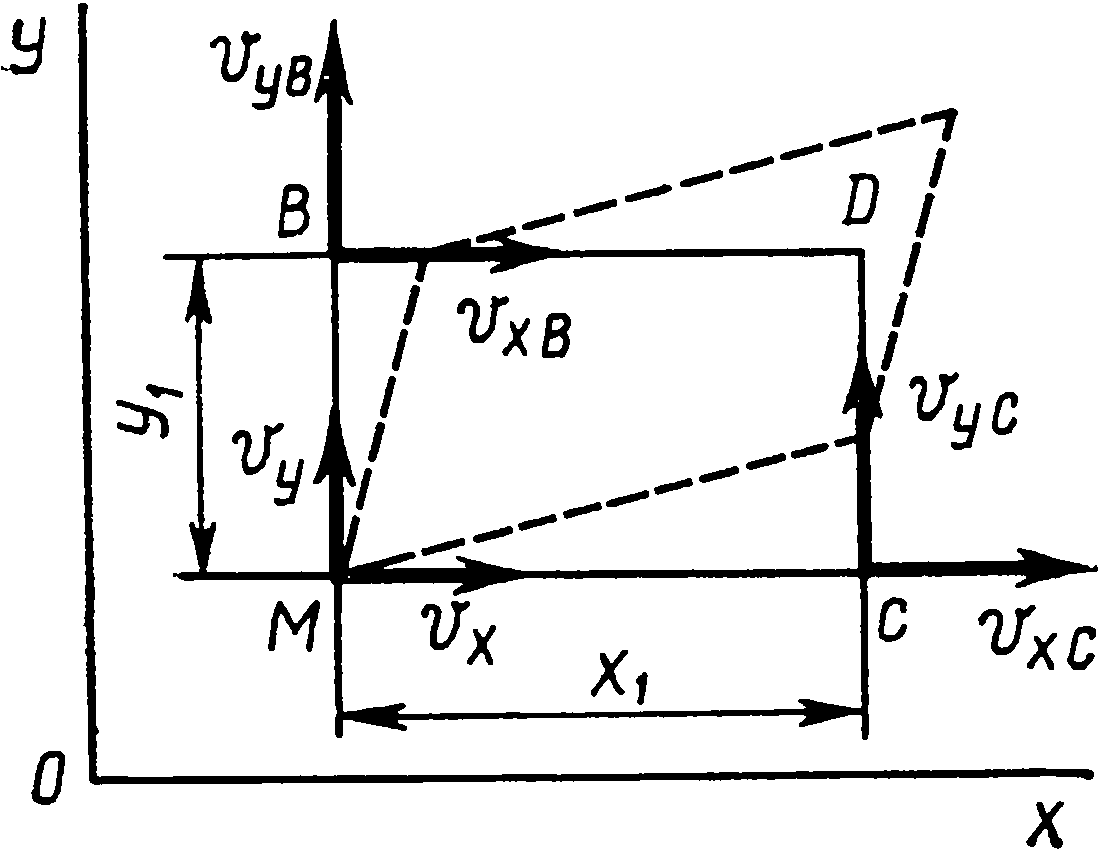
\includegraphics[width=0.3\linewidth]{img/deformation-of-fluid-part}
		\caption{Деформация частицы жидкости.}
		\label{fig:deformation-of-fluid-part}
	\end{figure}
	Пусть бесконечно малая жидкая частица имеет в момент времени $t$ форму прямоугольного параллелепипеда. Для упрощения рассмотрим проекцию этой частицы на плоскость $x,\; y$, т. е. бесконечно малый прямоугольник \textit{MBDC} (рис.~\ref{fig:deformation-of-fluid-part}). Если компоненты скорости в точке $M(x,\; y)$ прямоугольника обозначить $v_x,\; v_y$, то составляющие скорости в точках $C(x+x_1,\; y)$ и $B(x,\; y+y_1)$ можно представить в виде (с точностью до малых первого порядка)
	\begin{gather}
		\begin{dcases}\label{eq:222}
			v_{xC} = v_x + \frac{\pp v_x}{\pp x}x_1, \quad v_{yC} = v_y + \frac{\pp v_y}{\pp x}x_1;\\
			v_{xB} = v_x + \frac{\pp v_x}{\pp y}y_1, \quad v_{yB} = v_y + \frac{\pp v_y}{\pp y}y_1.
		\end{dcases}
	\end{gather}\n
	Поскольку рассматривается относительное перемещение точек \textit{C} и \textit{B} (относительно точки \textit{M}), приведем равенства \eqref{eq:222} в следующем виде:
	\begin{gather*}
		v_{xC} - v_x = \frac{\pp v_x}{\pp x}x_1, \quad v_{yC} - v_y = \frac{\pp v_y}{\pp x}x_1;\\
		v_{xB} - v_x = \frac{\pp v_x}{\pp y}y_1, \quad v_{yB} - v_y = \frac{\pp v_y}{\pp y}y_1.
	\end{gather*}\n
	Скорости $\frac{\pp v_x}{\pp x}x_1 = e_x x_1,\; \frac{\pp v_y}{\pp y}y_1 = e_y y_1$ являются скоростями линейной деформации ребер прямоугольника \textit{MBDC}; скорости $\frac{\pp v_y}{\pp x}x_1,\; \frac{\pp v_x}{\pp y}y_1$ указывают на поворот ребер \textit{MC} и \textit{MB} (рис.~\ref{fig:deformation-of-fluid-part}), т. е. являются скоростями деформации скашивания прямоугольника \textit{MBDC} в некоторый косоугольник (пунктир на рис.~\ref{fig:deformation-of-fluid-part}). Ребро \textit{MC} поворачивается с угловой скоростью ${\pp v_y}/{\pp x}$, а ребро \textit{MB} --- с угловой скоростью ${\pp v_x}/{\pp y}$. Так как скорость изменения прямого угла \textit{BMC} складывается из угловых скоростей вращения ребер \textit{MC} и \textit{MB}, то, следовательно, она представляет собой сумму: $\frac{\pp v_y}{\pp x} + \frac{\pp v_x}{\pp y} = 2\varepsilon_z$.\n
	Проводя аналогичные рассуждения для других граней параллелепипеда (или их проекций на координатные плоскости), можно так же показать, что величина $\frac{\pp v_z}{\pp z}z_1 = e_z z_1$ является скоростью линейной деформации вдоль оси $z$ и что значения угловых скоростей скашивания остальных прямых углов параллелепипеда выражаются соотношениями $\frac{\pp v_z}{\pp y} + \frac{\pp v_y}{\pp z} = 2\varepsilon_x$ и $\frac{\pp v_z}{\pp x} + \frac{\pp v_x}{\pp z} = 2\varepsilon_y$.\n
	Из изложенного следует, что величины ${\pp \varPhi}/{\pp x_1},\; {\pp \varPhi}/{\pp y_1},\; {\pp \varPhi}/{\pp z_1}$ действительно представляют собой компоненты скорости деформации жидкой частицы, причем величины $\varepsilon_x,\; \varepsilon_y,\; \varepsilon_z$ характеризуют деформацию скашивания, а величины $e_x,\; e_y,\; e_z$ --- линейную деформацию (растяжение или сжатие). Обращаясь вновь к формулам \eqref{eq:220}, физический смысл которых теперь полностью выяснен, можно сделать следующий вывод.\n
	\textit{Элементарное перемещение частицы жидкости (газа) состоит из поступательного перемещения ее центра со скоростью $\vv{v}\left(v_x,\; v_y,\; v_z\right)$ вращения относительно некоторой оси, проходящей через этот центр с угловой скоростью $\vv{\omega}\left(\omega_x,\; \omega_y,\; \omega_z\right)$, и деформационного движения, характеризуемого функцией $\varPhi\left(x_1,\; y_1,\; z_1\right)$.}
	
	\subsection{Понятие о потенциальном течении}
	\textit{Потенциальным движением жидкости называется безвихревое движение, т. е. такое движение, в котором компоненты вихря $\omega_x,\; \omega_y,\; \omega_z$ равны нулю.} Из условия отсутствия вихрей
	\begin{gather*}
		\omega_x = \frac{1}{2}\left(\frac{\pp v_z}{\pp y} - \frac{\pp v_y}{\pp z}\right) = 0,\quad
		\omega_y = \frac{1}{2}\left(\frac{\pp v_x}{\pp z} - \frac{\pp v_z}{\pp x}\right) = 0,\quad
		\omega_z = \frac{1}{2}\left(\frac{\pp v_y}{\pp x} - \frac{\pp v_x}{\pp y}\right) = 0
	\end{gather*}
	следует, что
	\begin{gather}\label{eq:223}
		\frac{\pp v_z}{\pp y} = \frac{\pp v_y}{\pp z},\quad
		\frac{\pp v_x}{\pp z} = \frac{\pp v_z}{\pp x},\quad
		\frac{\pp v_y}{\pp x} = \frac{\pp v_x}{\pp y}.
	\end{gather}\n
	Рассмотрим теперь дифференциальный трехчлен $v_x\dd x + v_y\dd y + v_z\dd z$. Как известно, равенства \eqref{eq:223} являются необходимыми и достаточными условиями того, чтобы этот дифференциальный трехчлен был полным дифференциалом некоторой функции, т. е. $v_x\dd x + v_y\dd y + v_z\dd z = \dd\varphi\left(x,\; y,\; z\right)$.\n
	Функцию $\varphi$ называют \textit{потенциалом скорости}. Раскрывая полный дифференциал $\dd\varphi$, т. е. $v_x\dd x + v_y\dd y + v_z\dd z = \frac{\pp\varphi}{\pp x}\dd x + \frac{\pp\varphi}{\pp y}\dd y + \frac{\pp\varphi}{\pp z}\dd z$, и сравнивая компоненты при $\dd x,\; \dd y,\; \dd z$, имеем
	\begin{gather}\label{eq:224}
		v_x = \frac{\pp\varphi}{\pp x},\quad
		v_y = \frac{\pp\varphi}{\pp y},\quad
		v_z = \frac{\pp\varphi}{\pp z},
	\end{gather}
	т. е. \textit{проекция скорости на координатную ось равна частной производной от потенциала скорости по соответствующей координате}.\n
	Это важное свойство потенциала скорости сохраняется и для произвольного направления, т. е. \textit{проекция скорости на произвольное направление равна производной от потенциала скорости по этому направлению}.
	
	\newpage
	\section{Лекция 3}
	
	\subsection{Основы теории вихрей}
	
	\subsubsection{Вихревая линия}
	\begin{figure}[htbp]
		\centering
		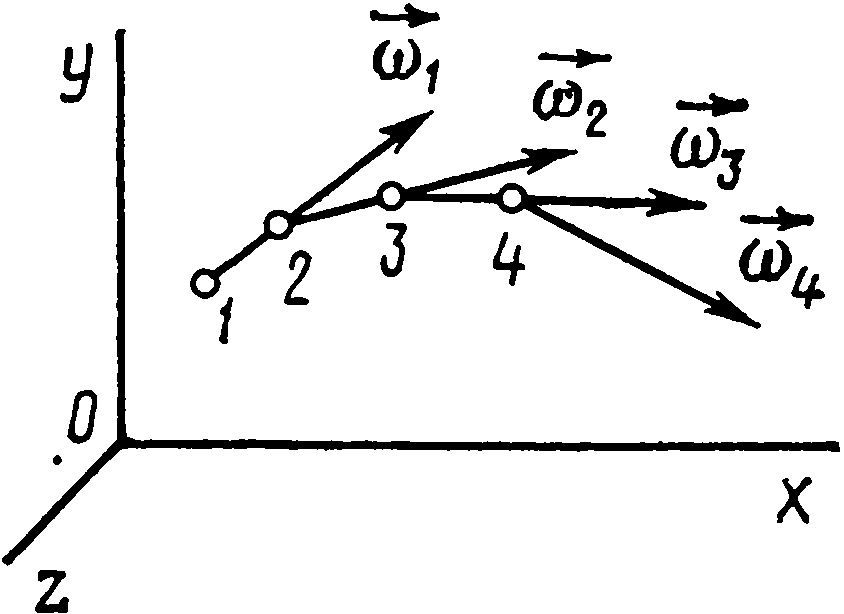
\includegraphics[width=0.25\linewidth]{img/vortex-line-construction}
		\caption{Построение вихревой линии.}
		\label{fig:2.6_vortex-line-construction}
	\end{figure}
	Вращательные движения частиц характеризуются угловыми скоростями:
	\begin{gather}
		\begin{dcases}\label{eq:225}
			\omega_x = \frac{1}{2}\left(\frac{\pp v_z}{\pp y} - \frac{\pp v_y}{\pp z}\right);\\
			\omega_y = \frac{1}{2}\left(\frac{\pp v_x}{\pp z} - \frac{\pp v_z}{\pp x}\right);\\
			\omega_z = \frac{1}{2}\left(\frac{\pp v_y}{\pp x} - \frac{\pp v_x}{\pp y}\right).
		\end{dcases}
	\end{gather}\n
	Это означает, что в каждой точке пространства вращение жидких частиц можно охарактеризовать вектором угловой скорости $\vv{\omega}$, модуль которого
	\begin{gather}
		\omega = \sqrt{\omega_x^2 + \omega_y^2 + \omega_z^2}.\label{eq:226}
	\end{gather}\n
	Каждый такой вектор $\vv{\omega}$ характеризует местное вращение жидкости (газа). Допустим, что в данный момент времени $t$ в какой-либо точке \textit{1} вектор угловой скорости равен $\vv{\omega_1}$ (рис.~\ref{fig:2.6_vortex-line-construction}). Возьмем в этот же момент времени на этом векторе близкую к точке \textit{1} точку \textit{2} и построим соответствующий ей вектор угловой скорости $\vv{\omega_2}$. Продолжая это построение, в данный момент времени получим ломаную линию \textit{1-2-3-4-\dots}, которая в пределе, т. е. при стремлении длины каждого звена ломаной к нулю превращается в так называемую вихревую линию. \textit{Вихревой линией называется линия, проведенная в данный момент времени в потоке жидкости (газа), в каждой точке которой вектор угловой скорости касателен к ней.}\n
	Дифференциальное уравнение вихревых линий имеет вид
	\begin{gather}
		\frac{\dd x}{\omega_x} = \frac{\dd y}{\omega_y} = \frac{\dd z}{\omega_z}.\label{eq:227}
	\end{gather}
	
	\subsubsection{Вихревая трубка}
	\begin{figure}[htbp]
		\centering
		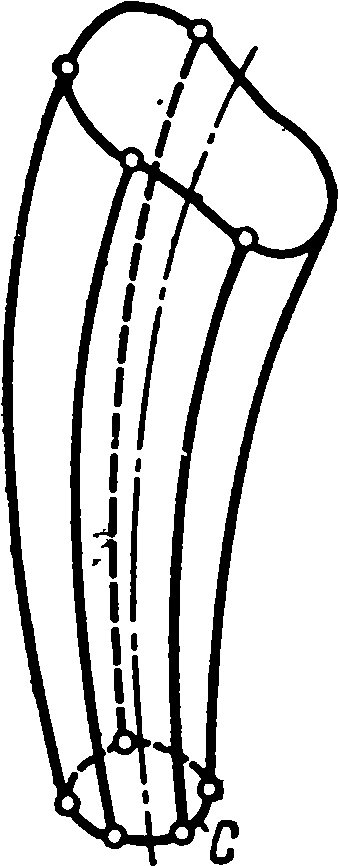
\includegraphics[width=0.1\linewidth]{img/vortex-tube}
		\caption{Вихревая трубка.}
		\label{fig:2.7_vortex-tube}
	\end{figure}
	Рассмотрим произвольный малый замкнутый контур \textit{C}, не являющийся вихревой линией, и проведем через каждую точку этого контура вихревую линию. Тогда совокупность этих линий образует поверхность, называемую \textit{вихревой трубкой} (рис.~\ref{fig:2.7_vortex-tube}). Жидкость (газ), заключенная в ней, называется \textit{вихревым шнуром, вихревой нитью или вихрем}. Под \textit{напряжением или интенсивностью} вихря понимают величину $\chi = 2\iint_\sigma \omega\dd\sigma$, где $\sigma$ --- площадь нормального (поперечного) сечения вихревой трубки. Пренебрегая изменением $\omega$ по сечению вихревой трубки, получим
	\begin{gather}
		\chi = 2 \omega \sigma.\label{eq:228}
	\end{gather}\n
	Значение напряжения (интенсивности) вихря $\chi$ связано с возникающей вокруг вихря циркуляцией $\Gamma$. Установлению этой связи посвящена теорема Стокса.\n
	
	\subsubsection{Теорема Стокса}
	\begin{theorem}[Случай теоремы Стокса для элементарного замкнутого контура]\label{thm:Stokes-1}
		Циркуляция по бесконечно малому прямоугольному контуру равна напряжению вихря, пронизывающего этот контур:
		\begin{gather*}
			\dd \Gamma = 2 \omega_n \dd \sigma,
		\end{gather*}
		где $\omega_n$ --- проекция угловой скорости $\vv{\omega}$ на нормаль к произвольно расположенной в пространстве бесконечно малой прямоугольной площадке $\dd \sigma$.
	\end{theorem}
	\begin{proof}
		\begin{figure}[htbp]
			\centering
			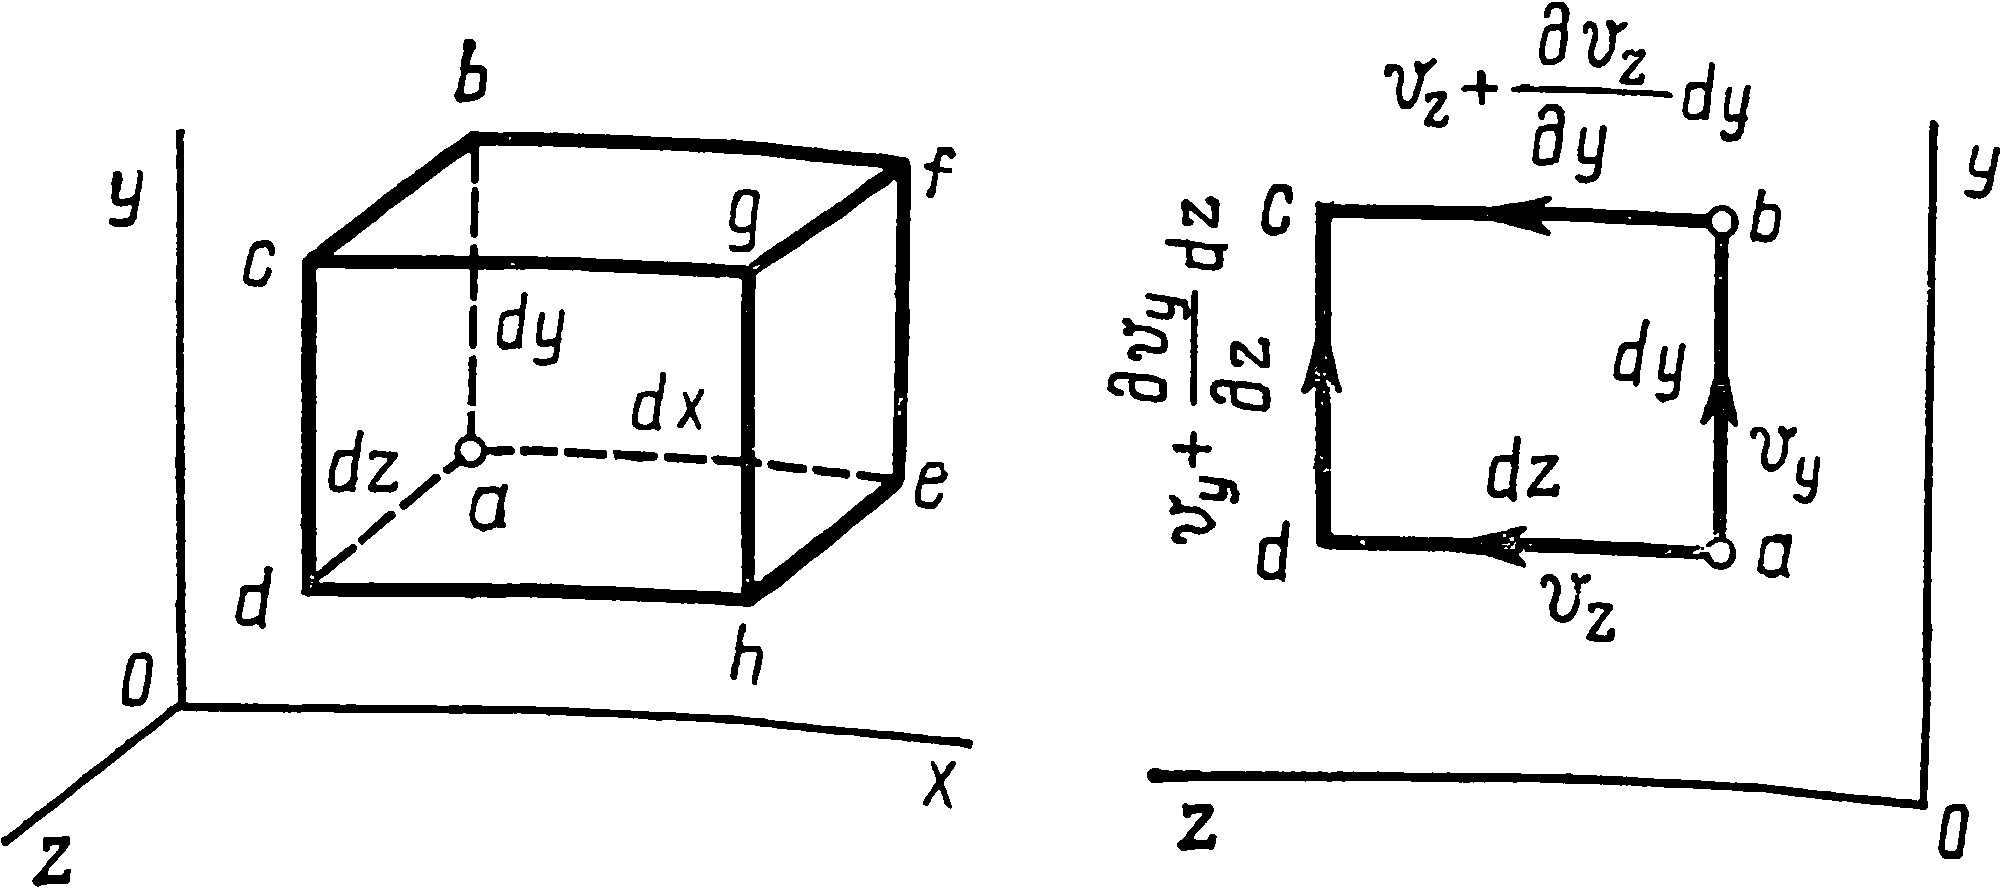
\includegraphics[width=0.75\linewidth]{img/circulation-calculation-scheme}
			\caption{Схема вычисления циркуляции по бесконечно малому прямоугольному контуру.}
			\label{fig:2.8_circulation-calculation-scheme}
		\end{figure}
		Рассмотрим в движущейся жидкости вихревое поле, т. е. предположим, что в жидкости непрерывно распределены вихри (векторы $\vv{\omega}$). Выделим бесконечно малый объем в форме прямоугольного параллелепипеда с ребрами $\dd x,\; \dd y,\; \dd z$ (рис.~\ref{fig:2.8_circulation-calculation-scheme}). Рассмотрим в плоскости \textit{yz} бесконечно малый прямоугольник \textit{abcda} со сторонами $\dd y$ и $\dd z$, являющийся проекцией рассматриваемого параллелепипеда на плоскость \textit{yz}. Подсчитаем циркуляцию $\Gamma_x$ по элементарному контуру \textit{abcda}, приписывая индексу $x$ смысл обхода вокруг оси, параллельной оси \textit{x}.\n
		Пусть $v_y$ и $v_z$ --- проекции вектора скорости точки \textit{a} на оси \textit{y}, \textit{z}. Подсчитаем значения скоростей, направленных вдоль сторон \textit{bc} и \textit{dc} в точках \textit{b} и \textit{d}, т. е.
		\begin{gather*}
			\left(v_z\right)_b = v_z + \frac{\pp v_z}{\pp y} \dd y, \quad \left(v_y\right)_d = v_y + \frac{\pp v_y}{\pp z} \dd z.
		\end{gather*}\n
		Циркуляция $\dd\Gamma_x$ по контуру \textit{abcda} складывается из циркуляций вдоль бесконечно малых сторон, равных произведению скорости на длины соответствующих сторон прямоугольника. Таким образом,
		\begin{gather*}
			\dd\Gamma_x = v_y\dd y + \left[v_z + \frac{\pp v_z}{\pp y} \dd y\right]\dd z - \left[v_y + \frac{\pp v_y}{\pp z} \dd z\right]\dd y - v_z\dd z.
		\end{gather*}\n
		Знак <<-->> вдоль сторон \textit{cd} и \textit{ca} берется потому, что направление обхода обратно направлению скорости. Отсюда
		\begin{gather*}
			\dd\Gamma_x = \left(\frac{\pp v_z}{\pp y} - \frac{\pp v_y}{\pp z}\right)\dd y \dd z,
		\end{gather*}
		или, обозначая $\dd y \dd z = \dd \sigma_x$, получаем
		\begin{gather}
			\dd\Gamma_x = 2\omega_x\dd\sigma_x.\label{eq:229а}
		\end{gather}\n
		Аналогично, для контуров, расположенных в плоскостях, перпендикулярных осям \textit{у} и \textit{z},
		\begin{gather}
			\dd\Gamma_y = 2\omega_y\dd\sigma_y;\label{eq:229б}\\
			\dd\Gamma_z = 2\omega_z\dd\sigma_z.\label{eq:229в}
		\end{gather}\n
		Распространяя полученный результат на произвольно расположенную в пространстве бесконечно малую прямоугольную площадку $\dd\sigma$, имеем
		\begin{gather}
			\dd \Gamma = 2 \omega_n \dd \sigma,\label{eq:230}
		\end{gather}
		где $\omega_n$ --- проекция угловой скорости $\vv{\omega}$ на нормаль к площадке.
	\end{proof}\n
	Соотношение \eqref{eq:230} между циркуляцией скорости по замкнутому контуру и интенсивностью вихря, охватываемого контуром, может быть обобщено на случай контура конечных размеров.
	\begin{theorem}[теорема Стокса, интегральная формула Стокса]\label{thm:Stokes-2}
		Циркуляция скорости по замкнутому односвязному контуру \textit{L} равна удвоенному интегралу от интенсивностей вихрей, проходящих сквозь незамкнутую поверхность, ограниченную контуром:
		\begin{gather*}
			\Gamma = 2 \int\limits_{\left(S\right)} \omega_n \dd S.
		\end{gather*}
	\end{theorem}
	\begin{proof}
		\begin{figure}[htbp]
			\centering
			\begin{minipage}{0.32\textwidth}
				\centering
				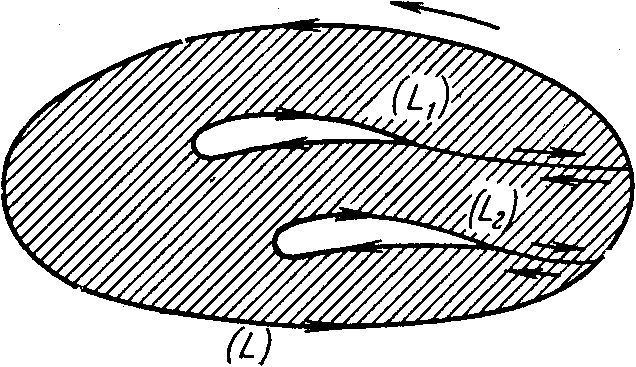
\includegraphics[width=0.95\textwidth]{img/3-linked-region-example}
				\captionof{figure}{Пример трехсвязной области на плоскости. Разрезы преобразуют область в односвязную.}
				\label{fig:4.58_3-linked-region-example}
			\end{minipage}
			\hfill
			\begin{minipage}{0.32\textwidth}
				\centering
				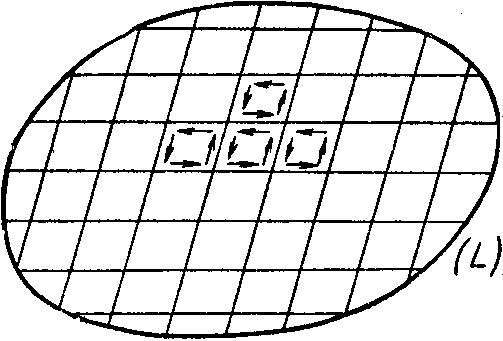
\includegraphics[width=0.95\textwidth]{img/to-Stokes-proof}
				\captionof{figure}{К доказательству теоремы Стокса о циркуляции скорости по замкнутому контуру.}
				\label{fig:4.59_to-Stokes-proof}
			\end{minipage}
			\hfill
			\begin{minipage}{0.32\textwidth}
				\centering
				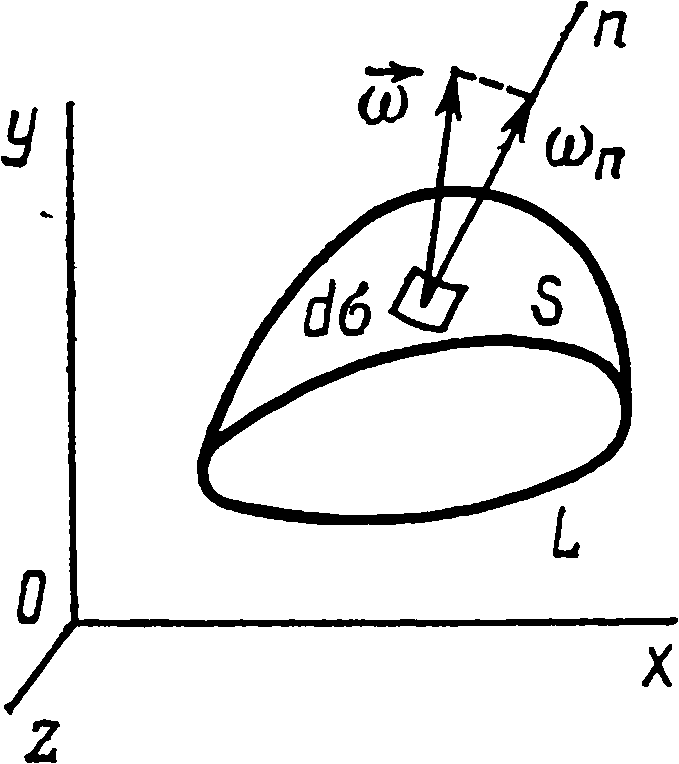
\includegraphics[width=0.75\textwidth]{img/vortex-flow-surface}
				\captionof{figure}{Произвольная поверхность, пронизываемая потоком вихрей.}
				\label{fig:2.10_vortex-flow-surface}
			\end{minipage}
		\end{figure}
		Пусть \textit{L} есть произвольный замкнутый контур, ограничивающий некоторую поверхность \textit{S}. Предположим, что поверхность \textit{S} ограничена только контуром \textit{L}, т. е. что внутри контура \textit{L} нет других контуров, ограничивающих поверхность \textit{S}, как, например, в случае поверхности, изображенной на рис.~\ref{fig:4.58_3-linked-region-example}. Предположим, говоря проще, что внутри области, ограниченной контуром \textit{L}, нет <<дыр>>. Такая поверхность называется \textit{односвязной}. Проведем вспомогательные линии так, чтобы разделить эту область на элементарные площадки. Для каждой (\textit{i}-й) площадки, согласно \eqref{eq:230}:
		\begin{gather*}
			\dd\Gamma_i = 2\omega_{ni}\dd\sigma_i \quad \left(i = 1,\; 2,\; 3,\; \dots,\; m\right).
		\end{gather*}
		Просуммируем эти равенства по всем \textit{m} площадкам:
		\begin{gather*}
			\sum_{i\,=\,1}^{m}\dd\Gamma_i = 2\sum_{i\,=\,1}^{m}\omega_{ni}\dd\sigma_i.
		\end{gather*}\n
		Здесь сумма в левой части представляет собой циркуляцию скорости $\Gamma$ по контуру \textit{L}. В самом деле, каждый из элементарных контуров, образованных вспомогательными линиями, будет при суммировании пройден дважды в обратных друг другу направлениях, ибо всякий участок такого контура принадлежит двум соседним площадкам. Следовательно, произведения $v_s\dd s$ для всех вспомогательных линий взаимно сократятся. Останутся в левой части после сокращения лишь произведения $v_s\dd s$, относящиеся к элементам контура \textit{L}, а они в сумме как раз и дадут, по определению, циркуляцию скорости по этому контуру. Таким образом, при любом разделении области на элементарные площадки циркуляция скорости по контуру \textit{L} равна
		\begin{gather*}
			\Gamma = 2\sum_{i\,=\,1}^{m}\omega_{ni}\dd\sigma_i.
		\end{gather*}\n
		В пределе, при увеличении числа элементарных площадок до бесконечности ($m\rightarrow\infty$) и одновременном уменьшении всех $\dd\sigma_i$ до нуля, средние значения $\omega_{ni}$ будут равны значениям этой величины в соответствующих точках, а сумма в правой части будет равна $\int_{\left(S\right)}\omega_n\dd S$. Левая часть при этом переходе к пределу, по доказанному, не изменяется. В результате получаем следующее выражение для циркуляции скорости по замкнутому контуру конечных размеров:
		\begin{gather}
			\Gamma = 2 \int\limits_{\left(S\right)} \omega_n \dd S.\label{eq:479}
		\end{gather}
	\end{proof}
	Если вместо $\Gamma$ подставить его выражение через контурный интеграл (по формуле~\eqref{eq:210}), то из последнего соотношения получим общую формулу, выражающую контурный интеграл по контуру \textit{L} через двойной, взятый по поверхности \textit{S}, ограниченной контуром \textit{L}:
	\begin{gather}
		\oint\limits_{\left(L\right)} v_s\dd s = 2\oint\limits_{\left(S\right)}\omega_n\dd S.\label{eq:480}
	\end{gather}\n
	Теорему Стокса, выражаемую равенством \eqref{eq:479} или \eqref{eq:480}, можно распространить и на случай многосвязной области. Для этого нужно соединить вспомогательными линиями (разрезами) наружный контур с внутренними так, чтобы получилась односвязная область.\n
	Двойной интеграл в правой части распространяется в этом случае на заштрихованную область (рис.~\ref{fig:4.58_3-linked-region-example}), а контурный интеграл берется не только по наружному контуру \textit{L}, но также вдоль разрезов и по всем внутренним контурам. При этом за положительное направление обхода по всем контурам принимается такое, когда при обходе заштрихованная область остается по левую сторону.\n
	Так как разрезы при вычислении циркуляции проходятся дважды в противоположных направлениях, то интегралы, взятые вдоль разрезов, взаимно сократятся и останутся лишь циркуляции скорости $\Gamma_{L_1}$ и $\Gamma_{L_2}$ по внутренним контурам. В результате применения теоремы Стокса получим:
	\begin{gather*}
		\Gamma_L - \Gamma_{L_1} - \Gamma_{L_2} = 2\int\limits_{\left(S\right)}\omega_n\dd S.
	\end{gather*}
	Величины $\Gamma_{L_1}$ и $\Gamma_{L_2}$ входят в последнее равенство со знаком минус потому, что положительное направление обхода по каждому внутреннему контуру (когда находящаяся внутри него область остается по левую сторону) противоположно положительному направлению обхода по этому контуру, когда он присоединен с помощью разреза к наружному контуру. Из последнего равенства следует, что для трехсвязной области
	\begin{gather*}
		\Gamma_L = 2\int\limits_{\left(S\right)}\omega_n\dd S + \Gamma_{L_1} + \Gamma_{L_2}.
	\end{gather*}\n
	В общем случае, при наличии \textit{n} внутренних контуров циркуляция скорости по наружному контуру равна
	\begin{gather*}
		\Gamma_L = 2\int\limits_{\left(S\right)}\omega_n\dd S + \sum_{i\,=\,1}^{n}\Gamma_{L_i}.
	\end{gather*}
	\begin{figure}[htbp]
		\centering
		\hspace*{\fill}
		\begin{minipage}{0.4\textwidth}
			\centering
			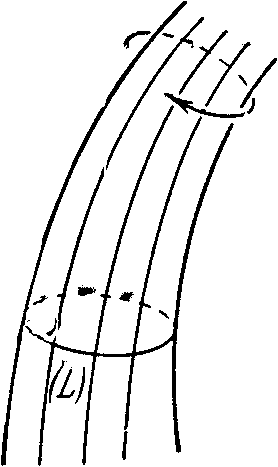
\includegraphics[width=0.35\textwidth]{img/closed-path-covers-tube}
			\captionof{figure}{Замкнутый контур \textit{L} охватывает вихревую трубку.}
			\label{fig:4.60_closed-path-covers-tube}
		\end{minipage}
		\hspace{5mm}
		\begin{minipage}{0.4\textwidth}
			\centering
			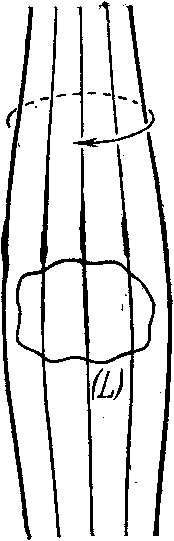
\includegraphics[width=0.2\textwidth]{img/closed-path-on-tube}
			\captionof{figure}{Замкнутый контур \textit{L} лежит на поверхности вихревой трубки, но ее не охватывает.}
			\label{fig:4.61_closed-path-on-tube}
		\end{minipage}
		\hspace*{\fill}
	\end{figure}
	\begin{corollary}\label{cor:Stokes-1}
		Если на поверхности вихревой трубки провести замкнутый контур, охватывающий вихревую трубку\footnote{То есть такой, который не может быть стянут в точку без того, чтобы не перерезать вихревую трубку.}) (рис.~\ref{fig:4.60_closed-path-covers-tube}), то циркуляция скорости по такому контуру равна удвоенной интенсивности вихревой трубки.
	\end{corollary}
	\begin{corollary}\label{cor:Stokes-2}
		Если на поверхности вихревой трубки провести замкнутый контур \textit{L}, не охватывающий трубку (рис.~\ref{fig:4.61_closed-path-on-tube}), то циркуляция скорости по такому контуру равна нулю.
	\end{corollary}
	В самом деле, во всех точках поверхности вихревой трубки, по ее определению, вектор угловой скорости частицы направлен по касательной к поверхности и, следовательно, составляющая этого вектора по нормали к поверхности $\omega_n=0$. В этом случае по теореме Стокса должна равняться нулю и циркуляция скорости.
	
	\subsubsection{Теоремы Гельмгольца о вихрях}
	\begin{theorem}[Вторая теорема Гельмгольца]\label{thm:Gelmgolts-2}
		Если силы, действующие в баротропной\footnote{Равновесие газа называется \textit{баротропным}, если плотность газа может быть рассматриваема как функция только давления ($\rho=\rho\left(p\right)$). В противном случае ($\rho=\rho\left(p,\; T\right)$) равновесие называют \textit{бароклинным}. Подробнее --- см. \cite{5}, \S28.} жидкости, имеют потенциал, то вихревая трубка во все время движения состоит из одних и тех же частиц жидкости.
	\end{theorem}
	Вторая теорема Гельмгольца устанавливает, что распространение вращательного движения на новые частицы жидкости или, наоборот, переход частиц от вращательного движения к потенциальному могут произойти в баротропной среде лишь под действием сил, не имеющих потенциала, в частности под действием сил трения.
	\begin{theorem}[Третья теорема Гельмгольца]\label{thm:Gelmgolts-3}
		Если силы, действующие в баротропной жидкости, имеют потенциал, то интенсивность вихревой трубки есть величина постоянная во все время движения.
	\end{theorem}
	Из третьей теоремы Гельмгольца следует, что изменение интенсивности вихрей в баротропной жидкости может происходить только от действия сил, не имеющих потенциала, например от действия сил трения.\n
	Если же баротропная жидкость идеальна\footnote{Для идеальной среды постулируется отсутствие касательных напряжений безотносительно к тому, покоится или движется среда. Принятое допущение равносильно условию отсутствия в идеальной среде \textit{внутреннего трения}. Подробнее --- см. \cite{5}, \S29.}, то интенсивности вихрей изменяться не могут, и в частности, если в идеальной жидкости вихри в какой-либо момент времени отсутствуют, т. е. движение во всех точках потенциально, то оно будет оставаться потенциальным во всякий другой момент времени. Последнее положение называется обычно \textit{теоремой Лагранжа}.
	\begin{proof}
		\begin{figure}
			\centering
			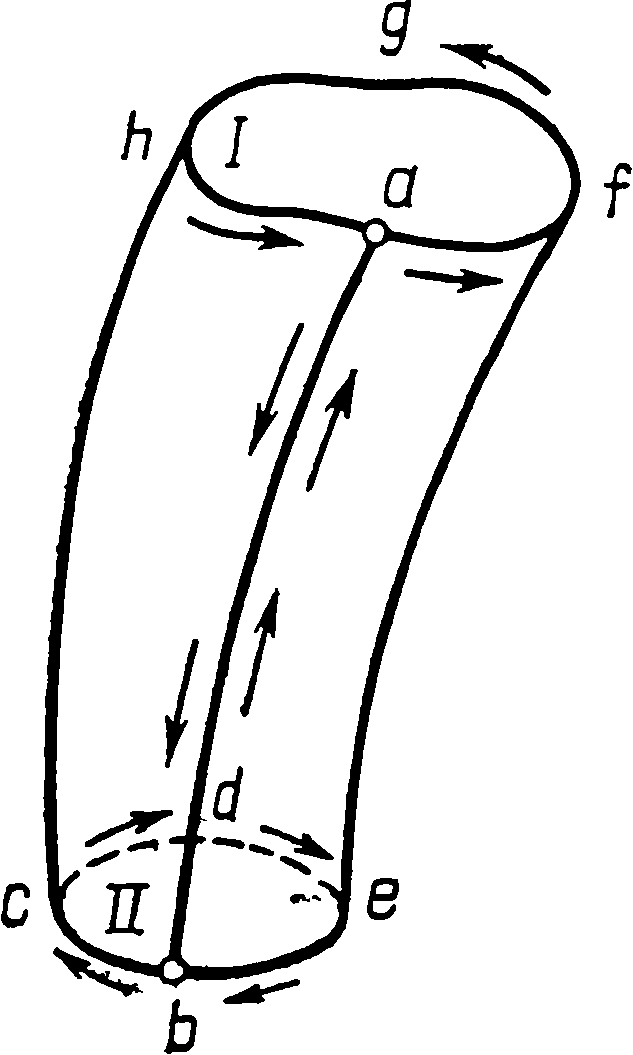
\includegraphics[width=0.15\linewidth]{img/path-on-vortex-tube}
			\caption{Контур, расположенный на поверхности вихревой трубки.}
			\label{fig:2.11_path-on-vortex-tube}
		\end{figure}
		Для доказательства рассмотрим часть вихревой трубки (рис.~\ref{fig:2.11_path-on-vortex-tube}), заключенную между двумя произвольными сечениями \textit{I} и \textit{II}. Очевидно, теорема будет доказана, если докажем, что напряжение в сечениях \textit{I} и \textit{II} одинаково, т. е. что $\chi_I = \chi_{II}$. Для этого соединим точки \textit{а} и \textit{b} обоих сечений произвольной линией \textit{ab}, лежащей на поверхности вихревой трубки, и рассмотрим циркуляцию по контуру \textit{abcdebafgha}. Так как этот контур является простым замкнутым контуром и лежит на поверхности вихревой трубки, то $\Gamma=0$. Но циркуляция по нему состоит из циркуляции по контурам \textit{I}, \textit{II} и линиям \textit{ab} и \textit{ba}. Следовательно, $\Gamma_I + \Gamma_{ab} - \Gamma_{II} + \Gamma_{ba} = 0$. Так как очевидно, что $\Gamma_{ab} = -\Gamma_{ba}$, то $\Gamma_I = \Gamma_{II}$ и, следовательно, на основании теоремы Стокса (\ref{thm:Stokes-2}) $\chi_I = \chi_{II}$.
	\end{proof}
	Из этой теоремы можно сделать вывод о возможных формах существования вихрей. Важным следствием этой теоремы является то, что из-за постоянства напряжения вдоль вихревой трубки вихрь не может обрываться в жидкости ($\sigma\neq=0$), так как в противном случае (при $\sigma=0$) $\omega\rightarrow\infty$, что физически невозможно.\n
	Вихри могут быть замкнутыми, образуя вихревые кольца, могут опираться на граничные области --- на поверхность твердого тела либо на поверхность раздела двух сред с различной плотностью. Вихри теоретически могут иметь также бесконечную протяженность. Однако форма существования вихря в виде бесконечного или полубесконечного вихревого шнура возможна только в невязком газе (в идеальной жидкости). В реальных условиях под действием вязкости вихрь постепенно разрушается (затухает).\n
	В невязком газе (идеальной жидкости), где отсутствуют касательные силы --- силы вязкости, тормозящие вращение, вихри не исчезают. По этой же причине в идеальной жидкости вихри не возникают. Рассматривая вихри в невязкой среде, изучают модель явления, причиной которого является вязкость.
	
	\subsubsection{Формула Био-Савара о вихревом влиянии}
	\begin{figure}[htbp]
		\centering
		\begin{minipage}{0.49\textwidth}
			\centering
			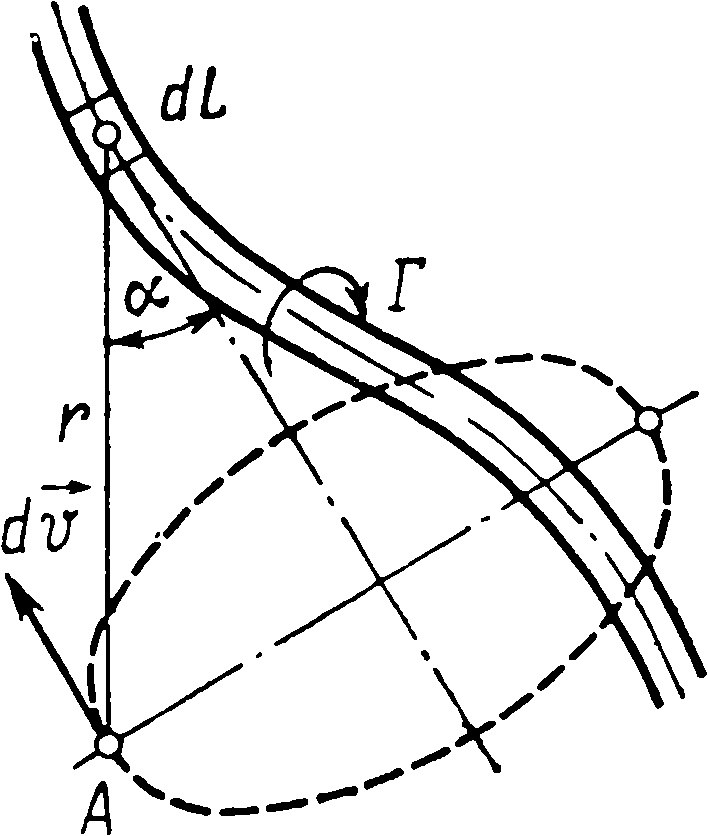
\includegraphics[width=0.5\textwidth]{img/vortex-influence-scheme}
			\captionof{figure}{Схема вихревого влияния.}
			\label{fig:2.12_vortex-influence-scheme}
		\end{minipage}
		\hfill
		\begin{minipage}{0.49\textwidth}
			\centering
			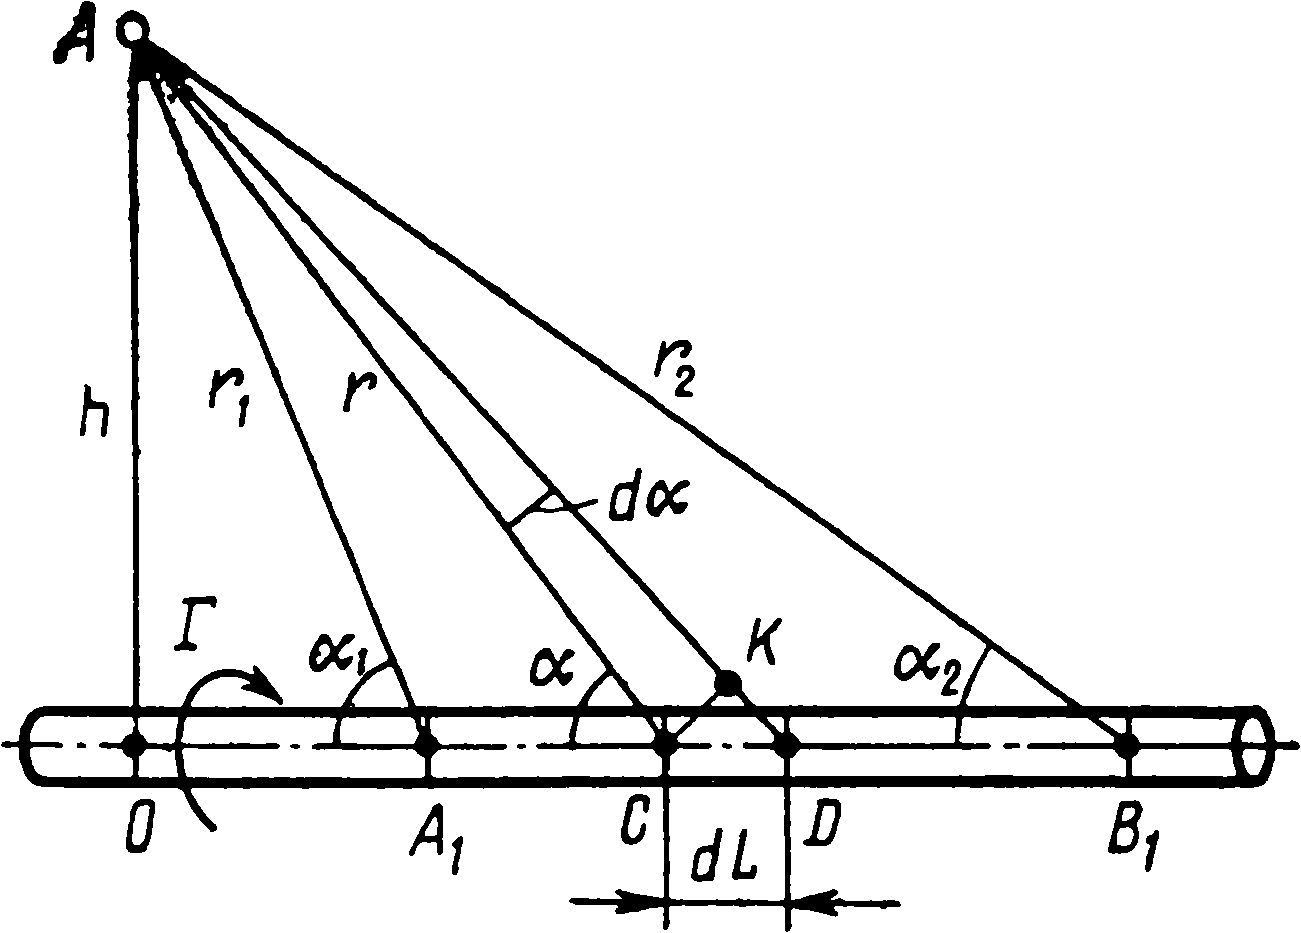
\includegraphics[width=0.75\textwidth]{img/vortex-velocity-definition-scheme}
			\captionof{figure}{Схема для определения скоростей, индуцируемых прямолинейным бесконечно длинным вихрем.}
			\label{fig:2.13_vortex-velocity-definition-scheme}
		\end{minipage}
	\end{figure}
	Найдем скорость, вызываемую вихрем произвольной формы с напряжением $\Gamma$ в какой-либо точке \textit{A} жидкости (рис.~\ref{fig:2.12_vortex-influence-scheme}). Для этого выделим элемент $\dd L$. Обозначим $r$ расстояние от точки \textit{A} до элемента $\dd L$; $\alpha$ --- угол, образуемый радиусом $r$ с касательной к оси элемента вихря $\dd L$. Тогда скорость $\dd v$, индуцируемая элементом вихря $\dd L$ в точке \textit{A},
	\begin{gather}
		\dd v = \frac{\Gamma}{4 \pi r^2}\sin\alpha \dd L.\label{eq:232}
	\end{gather}
	Эта формула носит название \textit{формулы Био-Савара}.\n
	Для определения полной скорости, индуцируемой всем вихрем в точке \textit{A}, выражение \eqref{eq:232} надо проинтегрировать по длине вихря:
	\begin{gather}
		v = \frac{\Gamma}{4 \pi} \int\limits_L \frac{\sin\alpha}{r^2} \dd L.\label{eq:233}
	\end{gather}\n
	Применим формулу \eqref{eq:233} к случаю бесконечно длинного прямолинейного вихря с напряжением $\chi = \Gamma$. Сначала найдем скорость $v$, индуцируемую в точке \textit{A} конечным участком этого вихря (рис.~\ref{fig:2.13_vortex-velocity-definition-scheme}).\n
	Радиус-векторы $r_1,\; r_2$ и углы $\alpha_1,\; \alpha_2$, соответствующие точкам $A_1,\; B_1$, а также длину перпендикуляра $h$, опущенного из точки \textit{A} на ось вихря, считаем заданными (задана также и величина $\Gamma$). Выделим на участке $A_1 B_1$ вихря бесконечно малый элемент $\text{\textit{CD}} = \dd L$. Из треугольников \textit{CKD} и \textit{CAK} находим $\text{\textit{CD}} = \dd L = \frac{r \dd\alpha}{\sin\alpha}$.\n
	С другой стороны, из треугольника \textit{OAC} имеем $r = h/\sin\alpha$.\n
	Подставляя значения $r$ и $\dd L$ в формулу \eqref{eq:232}, получаем
	\begin{gather*}
		\dd v = \frac{\Gamma}{4\pi h}\sin\alpha\dd\alpha.
	\end{gather*}\n
	Для определения скорости, индуцируемой вихрем $A_1 B_1$ в точке \textit{A}, это выражение надо проинтегрировать в пределах от $\alpha_2$, до $\alpha_1$. Тогда
	\begin{gather}
		v = \frac{\Gamma}{4\pi h}\left(\cos\alpha_2 - \cos\alpha_1\right).\label{eq:234}
	\end{gather}\n
	Обозначая $OA_1 = x_1$ и $OB_1 = x_2$, формуле \eqref{eq:234} можно придать вид
	\begin{gather}
		v = \frac{\Gamma}{4\pi h}\left(\frac{x_2}{\sqrt{x_2^2+h^2}} - \frac{x_1}{\sqrt{x_1^2+h^2}}\right).\label{eq:235}
	\end{gather}\n
	Рассмотрим два частных случая.
	\paragraph{Первый случай} Полубесконечный вихрь, простирающийся от точки \textit{O} до бесконечности. При этом $\alpha_1 = \pi/2,\; \alpha_2 = 0$ и, следовательно,
	\begin{gather}
		v = \frac{\Gamma}{4\pi h}.\label{eq:236}
	\end{gather}
	\paragraph{Второй случай} Бесконечно длинный вихревой шнур, простирающийся в обе стороны до бесконечности. При этом $\alpha_1 = \pi,\; \alpha_2 = 0$ и формула \eqref{eq:234} принимает вид
	\begin{gather}
		v = \frac{\Gamma}{2\pi h}.\label{eq:237}
	\end{gather}
	
	\newpage
	\part{Динамика жидкости и газа}
	
	\section{Лекция 4}
	
	\subsection{Основные уравнения жидкости и газа}
	Рассмотрим произвольное пространственное неустановившееся течение газа. В этом случае при заданных массовых силах движение газа можно считать известным, если известны три проекции скорости потока $v_x,\; v_y,\; v_z$ и параметры состояния газа --- давление $p$, плотность $\rho$ и температура $T$.\n
	Для определения шести указанных неизвестных величин нужно составить шесть уравнений. Выведем основные уравнения движения газа. При этом будем пользоваться методом Эйлера, в котором исследуется изменение $v_x,\; v_y,\; v_z,\; p,\; \rho,\; T$ в зависимости от положения точки (координат $x,\; y,\; z$) и времени. Для установившегося движения эти величины зависят только от координат.\n
	Для того чтобы сформулировать общие законы механики применительно к жидкой или газообразной среде, \textit{необходимо выделить в этой среде некоторую ее часть и заменить действие окружающей ее среды соответствующими силами}. В том случае, когда в результате решения задачи должны быть известны распределенные характеристики (распределение скорости и давления), применяется \textit{метод элементарных объемов}. При этом из жидкой или газообразной среды выделяется элементарный объем, в пределах которого изменением скорости и плотности можно пренебречь. Применительно к этому объему можно составить соответствующие уравнения механики, относящиеся к динамике точки. Тогда в результате \textit{предельного перехода} при стягивании элементарного объема в точку получаются дифференциальные уравнения движения.\n
	При составлении дифференциальных уравнений искомые функции (скорость, давление, плотность) предполагаются непрерывными дифференцируемыми функциями координат.
	
	\subsection{Уравнение неразрывности}
	\begin{figure}[htbp]
		\centering
		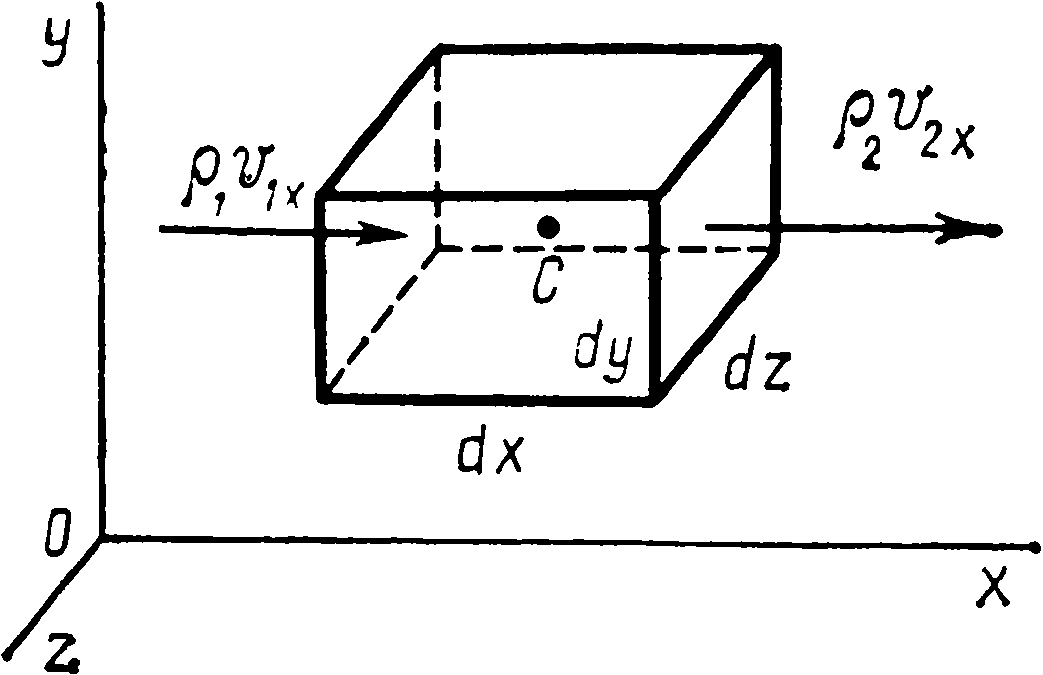
\includegraphics[width=0.3\linewidth]{img/continuity-equation-scheme}
		\caption{Схема для вывода уравнения неразрывности.}
		\label{fig:3.1_continuity-equation-scheme}
	\end{figure}
	Уравнение неразрывности представляет собой \textit{уравнение сохранения массы применительно к неразрывным течениям жидкости и газа}.\n
	Для вывода этого уравнения рассмотрим в потоке газа фиксированный в пространстве объем $V$ в виде прямоугольного параллелепипеда с ребрами $\dd x,\; \dd y,\; \dd z$, параллельными осям координат, и с центром в точке $C$ (рис.~\ref{fig:3.1_continuity-equation-scheme}). Обозначим $v_x,\; v_y,\; v_z,\; \rho$ составляющие скорости потока и плотность газа в точке $C$ в момент времени $t$. Масса газа, вытекающего из объема $V$ в направлении оси $x$ в единицу времени, $\left(\rho_2 v_{2x} - \rho_1 v_{1x}\right)\dd y\dd z$, где индексы 1 и 2 --- плотность и составляющие скорость $v_x$ на левой и правой гранях параллелепипеда.\n
	Так как $\rho v_x = f\left(x,\; y,\; z,\; t\right)$, то $\rho_2 v_{2x}$ и $\rho_1 v_{1x}$ с точностью до малых первого порядка можно представить в следующем виде:
	\begin{gather*}
		\rho_2 v_{2x} = f\left(x + \frac{\dd x}{2},\; y,\; z,\; t\right) = \rho v_x + \frac{\pp\left(\rho v_x\right)}{\pp x}\frac{\dd x}{2};\\
		\rho_1 v_{1x} = f\left(x - \frac{\dd x}{2},\; y,\; z,\; t\right) = \rho v_x - \frac{\pp\left(\rho v_x\right)}{\pp x}\frac{\dd x}{2}.
	\end{gather*}\n
	Тогда
	\begin{gather*}
		\left(\rho_2 v_{2x} - \rho_1 v_{1x}\right)\dd y\dd z = \frac{\pp\left(\rho v_x\right)}{\pp x}\dd x\dd y\dd z.
	\end{gather*}\n
	Аналогичные выражения можно привести для массы газа, вытекающего из параллелепипеда в направлении осей $y$ и $z$:
	\begin{gather*}
		\frac{\pp\left(\rho v_y\right)}{\pp y}\dd x\dd y\dd z, \quad \frac{\pp\left(\rho v_z\right)}{\pp z}\dd x\dd y\dd z.
	\end{gather*}\n
	Если эти выражения сложить, то получим суммарную массу газа, вытекающего из параллелепипеда в единицу времени:
	\begin{gather}
		\left[ \frac{\pp\left(\rho v_x\right)}{\pp x} + \frac{\pp\left(\rho v_y\right)}{\pp y} + \frac{\pp\left(\rho v_z\right)}{\pp z} \right]\dd x\dd y\dd z.\label{eq:31}
	\end{gather}\n
	Согласно закону сохранения массы для неразрывных течений, выражение \eqref{eq:31} должно быть равно изменению массы газа в объеме $V$ за единицу времени. Масса газа в объеме $V$ в момент времени $t$ равна $\rho\dd x\dd y\dd z$, a в момент времени $t + \dd t$ будет $\left[\rho + \frac{\pp\rho}{\pp t}\dd t\right]\dd x\dd y\dd z$.\n
	Следовательно, в единицу времени масса газа объема $V$ изменяется на величину
	\begin{gather}
		\frac{\pp\rho}{\pp t}\dd x\dd y\dd z,\label{eq:32}
	\end{gather}
	причем при положительном знаке выражения \eqref{eq:31} масса газа в объеме $V$ уменьшается, т. е. при этом $\frac{\pp\rho}{\pp t} < 0$. Приравнивая выражения \eqref{eq:31} и \eqref{eq:32} с учетом их знака, получаем
	\begin{gather*}
		\frac{\pp\left(\rho v_x\right)}{\pp x} + \frac{\pp\left(\rho v_y\right)}{\pp y} + \frac{\pp\left(\rho v_z\right)}{\pp z} = -\frac{\pp\rho}{\pp t}
	\end{gather*}
	или
	\begin{gather}
		\frac{\pp\rho}{\pp t} + \frac{\pp\left(\rho v_x\right)}{\pp x} + \frac{\pp\left(\rho v_y\right)}{\pp y} + \frac{\pp\left(\rho v_z\right)}{\pp z} = 0.\label{eq:33}
	\end{gather}\n
	Уравнение \eqref{eq:33} представляет собой \textit{уравнение неразрывности}. Его можно представить в виде
	\begin{subequations}
		\begin{gather}
			\frac{\pp\rho}{\pp t} + \diverg\footnotemark\left(\rho\vv{v}\right) = 0,\label{eq:34}
		\end{gather}
		или
		\begin{gather}
			\frac{1}{\rho}\frac{\dd\rho}{\dd t} + \diverg\left(\vv{v}\right) = 0.\label{eq:34'}
		\end{gather}
	\end{subequations}
	\footnotetext{Пусть векторное поле $\vv{a} = \left(a_x,\; a_y,\; a_z\right)$ дифференцируемо в некоторой точке. Число $\frac{\pp a_x}{\pp x} + \frac{\pp a_y}{\pp y} + \frac{\pp a_z}{\pp z}$ называется \textit{дивергенцией поля} в этой точке и обозначается через $\diverg{\vv{a}}$, т. е. $\diverg{\vv{a}} = \frac{\pp a_x}{\pp x} + \frac{\pp a_y}{\pp y} + \frac{\pp a_z}{\pp z}$. Точки векторного поля $\vv{a}$, в которых $\diverg\vv{a} \ne 0$ называются \textit{источниками} векторного поля. Подробнее --- см. \cite{3}, том 2, \S52.1, \S52.3.}
	
	\subsubsection{Случай установившегося движения}
	В частном случае установившегося движения $\frac{\pp\rho}{\pp t} = 0$. Тогда уравнение неразрывности приобретет вид
	\begin{gather}
		\frac{\pp\left(\rho v_x\right)}{\pp x} + \frac{\pp\left(\rho v_y\right)}{\pp y} + \frac{\pp\left(\rho v_z\right)}{\pp z} = 0;\label{eq:35}\\
		\diverg\left(\rho\vv{v}\right) = 0.\label{eq:36}
	\end{gather}
	
	\subsubsection{Случай несжимаемой среды}
	Для несжимаемой среды $\left(\rho = \mathrm{const}\right)$
	\begin{gather}
		\frac{\pp v_x}{\pp x} + \frac{\pp v_y}{\pp y} + \frac{\pp v_z}{\pp z} = 0;\label{eq:37}\\
		\diverg\vv{v} = 0.\label{eq:38}
	\end{gather}
	
	\subsubsection{Случай плоского потока}
	Выведем уравнения неразрывности применительно к плоскому потоку. В этом случае, принимая за плоскость потока плоскость $Oxy$, будем иметь $v_x\left(x,\; y,\; t\right)$, $v_y\left(x,\; y,\; t\right)$, $v_z = 0$, $\rho\left(x,\; y,\; t\right)$. Тогда вместо уравнений \eqref{eq:33}, \eqref{eq:35} и \eqref{eq:37} получим
	\begin{gather}
		\begin{dcases}\label{eq:39}
			\frac{\pp\rho}{\pp t} + \frac{\pp\left(\rho v_x\right)}{\pp x} + \frac{\pp\left(\rho v_y\right)}{\pp y} = 0;\\
			\frac{\pp\left(\rho v_x\right)}{\pp x} + \frac{\pp\left(\rho v_y\right)}{\pp y} = 0;\\
			\frac{\pp v_x}{\pp x} + \frac{\pp v_y}{\pp y} = 0.
		\end{dcases}
	\end{gather}
	
	\subsubsection{Уравнение неразрывности в сферической системе координат}
	Чтобы составить уравнения неразрывности в цилиндрических и сферических координатах, достаточно воспользоваться формулами для вычисления дивергенции в соответствующих системах координат.\n
	Приведем уравнение неразрывности для потока, обладающего осевой симметрией (осесимметричного потока --- см. п.~\ref{sec:fluid-moving-classification}), для которого во всех меридиональных плоскостях течения газа одинаковы. Рассмотрим сначала сферическую систему координат и воспользуемся выражением дивергенции в сферических координатах:
	\begin{gather}
		\diverg\left(\rho\vv{v}\right) = \frac{1}{r^2}\left[\frac{\pp}{\pp r}\left(r^2\rho v_r\right)\right] + \frac{1}{r \sin\varTheta}\frac{\pp \left(\rho v_\psi\right)}{\pp \psi} + \frac{1}{r \sin\varTheta}\left[\frac{\pp}{\pp\varTheta}\left(\sin\varTheta\rho v_\varTheta\right)\right],\label{eq:310}
	\end{gather}
	где $r$ --- длина радиус-вектора; $\varTheta$ --- полярный (зенитный) угол; $\psi$ --- долгота (азимутальный угол); $v_r$ --- радиальная компонента скорости; $v_\varTheta$ --- компонента скорости вдоль направления увеличения полярного угла; $v_\psi$ --- компонента скорости вдоль направления увеличения азимутального угла.\n
	В случае осесимметричного потока $v\psi = 0$, a $v_r$, $v_\varTheta$ и плотность $\rho$ зависят только от $r$, $\varTheta$ и $t$. Тогда из выражения \eqref{eq:310}
	\begin{gather*}
		\diverg\left(\rho\vv{v}\right) = \frac{\pp\left(\rho v_r\right)}{\pp r} + \frac{1}{r}\frac{\pp\left(\rho v_\varTheta\right)}{\pp\varTheta} + \frac{2}{r}\rho v_r + \frac{1}{r}\rho v_\varTheta\ctg\varTheta.
	\end{gather*}\n
	Подставляя это выражение в уравнения \eqref{eq:34} и \eqref{eq:36}, получаем уравнения неразрывности для неустановившегося и установившегося осесимметричного потока в следующем виде:
	\begin{gather}
		\begin{dcases}\label{eq:311}
			\frac{\pp\rho}{\pp t} + \frac{\pp\left(\rho v_r\right)}{\pp r} + \frac{1}{r}\frac{\pp\left(\rho v_\varTheta\right)}{\pp\varTheta} + \frac{2}{r}\rho v_r + \frac{1}{r}\rho v_\varTheta\ctg\varTheta = 0;\\
			r\frac{\pp\left(\rho v_r\right)}{\pp r} + \frac{\pp\left(\rho v_\varTheta\right)}{\pp\varTheta} + 2\rho v_r + \rho v_\varTheta\ctg\varTheta = 0.
		\end{dcases}
	\end{gather}
	
	\subsubsection{Уравнение неразрывности в цилиндрической системе координат}
	Аналогично, используя соответствующее выражение $\diverg\left(\rho\vv{v}\right)$, можно составить уравнение неразрывности в цилиндрических координатах. Для осесимметричного потока уравнение неразрывности в цилиндрических координатах имеет вид
	\begin{gather*}
		r\frac{\pp\rho}{\pp t} + \frac{\pp\left(r\rho v_x\right)}{\pp x} + \frac{\pp\left(r\rho v_r\right)}{\pp r} = 0.
	\end{gather*}\n
	Здесь $v_r$, $v_x$ --- составляющие скорости по осям цилиндрической системы координат.\n
	
	\subsubsection{Уравнение неразрывности в форме массового расхода}
	В случае установившегося одномерного движения газа можно пользоваться также уравнением неразрывности в форме массового расхода:
	\begin{gather*}
		\rho v F = \mathrm{const},
	\end{gather*}
	где $F$ --- площадь поперечного сечения трубки тока.\n
	
	\subsubsection{Уравнение неразрывности в форме объемного расхода}
	Для несжимаемой среды $\left(\rho = \mathrm{const}\right)$ это уравнение можно представить в форме объемного расхода:
	\begin{gather*}
		vF = \mathrm{const}.
	\end{gather*}
	
	\subsection{Дифференциальные уравнения движения невязкого газа (идеальной жидкости) в форме Эйлера}
	\begin{figure}[htbp]
		\centering
		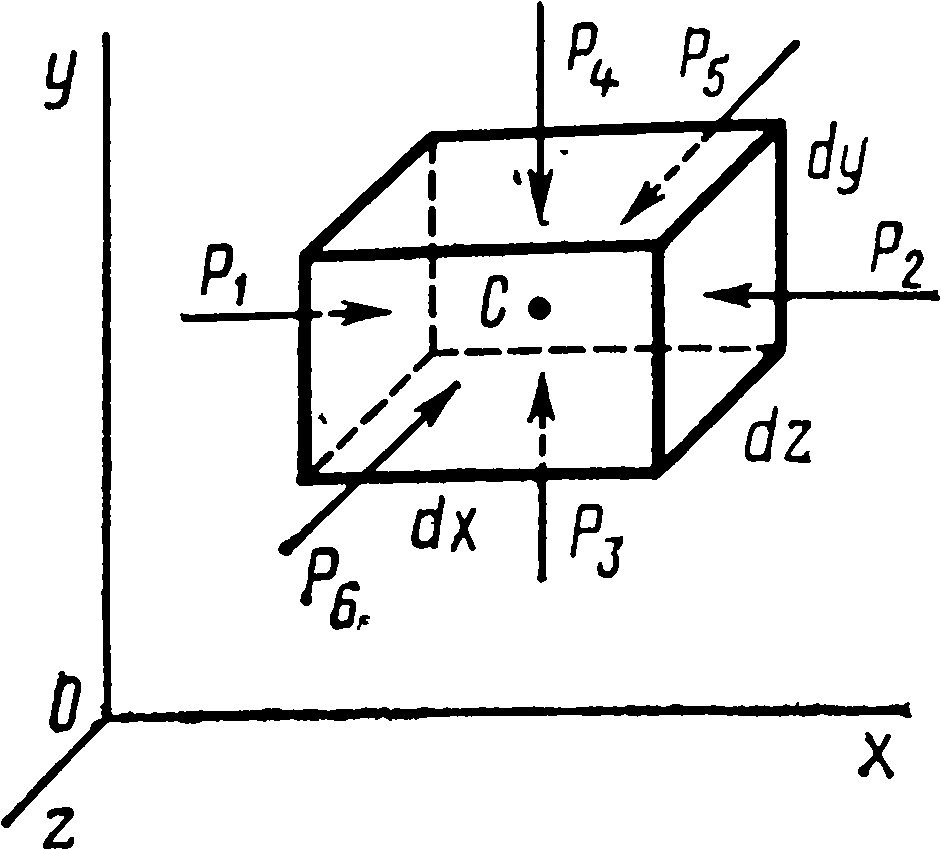
\includegraphics[width=0.3\linewidth]{img/surface-forces-on-ideal-fluid}
		\caption{Поверхностные силы, действующие на частицу идеальной жидкости.}
		\label{fig:3.2_surface-forces-on-ideal-fluid}
	\end{figure}
	Для вывода дифференциальных уравнений движения невязкого газа воспользуемся методом элементарных объемов и выделим в потоке малую частицу в форме прямоугольного параллелепипеда с центром в заданной точке пространства $C$ и с длинами ребер $\dd x$, $\dd y$, $\dd z$ (рис.~\ref{fig:3.2_surface-forces-on-ideal-fluid}). Масса частицы $\rho\dd x\dd y\dd z$. Применяя принцип Даламбера, рассмотрим равновесие сил, действующих на выделенную частицу. Силы, действующие в жидкости, можно представить в виде массовых и поверхностных сил. Следует отметить, что поверхностные силы при изучении движения газа являются основными.\n
	Массовые силы распределены по всему объему жидкости и пропорциональны массе рассматриваемой частицы. Обозначим $\vv{f}$ вектор массовой силы, отнесенной к единице массы, а $X$, $Y$, $Z$ --- его проекции на оси координат. Примером массовой силы является сила тяжести. При этом $X = 0$, $Y = -g$, $Z = 0$.\n
	Проекции массовой силы, действующей на данную частицу, в общем случае можно представить в виде $\rho X\dd x\dd y\dd z$, $\rho Y\dd x\dd y\dd z$, $\rho Z\dd x\dd y\dd z$.\n
	Со стороны окружающей среды на частицу действуют поверхностные силы, распределенные по граням параллелепипеда. В случае невязкой среды вектор поверхностной силы --- силы давления --- направлен по внутренней нормали к поверхности. Обозначим $p_1$, $p_2$ давления по граням, перпендикулярным оси $x$; $p_3$, $p_4$ и $p_5$, $p_6$ --- давления по граням, перпендикулярным осям $y$ и $z$. Тогда проекция поверхностных сил, действующих на частицу, в направлении оси $x$ будет равна $\left(p_1 - p_2\right)\dd y\dd z$, в точке $C$ давление $p = f\left(x,\; y,\; z,\; t\right)$. Давления на левой и правой гранях параллелепипеда с точностью до малых первого порядка могут быть представлены в следующем виде:
	\begin{gather*}
		p_1 = f\left(x - \frac{\dd x}{2},\; y,\; z,\; t\right) = p - \frac{\pp p}{\pp x}\frac{\dd x}{2};\\
		p_2 = f\left(x + \frac{\dd x}{2},\; y,\; z,\; t\right) = p + \frac{\pp p}{\pp x}\frac{\dd x}{2},
	\end{gather*}
	а суммарная проекция сил давления в направлении оси $x$ будет $-\frac{\pp p}{\pp x}\dd x\dd y\dd z$. Аналогично получим проекции сил давления на направления осей $y$ и $z$, т. е. $-\frac{\pp p}{\pp y}\dd x\dd y\dd z$, $-\frac{\pp p}{\pp z}\dd x\dd y\dd z$.\n
	Суммарные проекции всех сил, действующих на частицу, в направлении осей $x$, $y$, $z$:
	\begin{gather*}
		F_x = \left[X - \frac{1}{\rho}\frac{\pp p}{\pp x}\right]\rho\dd x\dd y\dd z;\\
		F_y = \left[Y - \frac{1}{\rho}\frac{\pp p}{\pp y}\right]\rho\dd x\dd y\dd z;\\
		F_z = \left[Z - \frac{1}{\rho}\frac{\pp p}{\pp z}\right]\rho\dd x\dd y\dd z.
	\end{gather*}\n
	Согласно принципу Даламбера, действующие на частицу поверхностные и массовые силы в каждый момент времени должны уравновешиваться силами инерции. Проекции инерционной силы:
	\begin{gather*}
		-\frac{\dd v_x}{\dd t}\rho\dd x\dd y\dd z, \quad -\frac{\dd v_y}{\dd t}\rho\dd x\dd y\dd z, \quad -\frac{\dd v_z}{\dd t}\rho\dd x\dd y\dd z.
	\end{gather*}\n
	Тогда, приравнивая проекции сил инерции проекциям суммарной силы, действующей на частицу, получим уравнения движения невязкой среды (идеальной жидкости) в форме Эйлера:
	\begin{subequations}
		\begin{gather}
			\begin{dcases}\label{eq:312}
				\frac{\dd v_x}{\dd t} = X - \frac{1}{\rho}\frac{\pp p}{\pp x};\\
				\frac{\dd v_y}{\dd t} = Y - \frac{1}{\rho}\frac{\pp p}{\pp y};\\
				\frac{\dd v_z}{\dd t} = Z - \frac{1}{\rho}\frac{\pp p}{\pp z}.
			\end{dcases}
		\end{gather}\n
		Уравнения \eqref{eq:312} применимы для исследования движения как сжимаемой, так и несжимаемой среды. Каждый член уравнений представляет собой ускорение: $\frac{\dd v_x}{\dd t}$, $\frac{\dd v_y}{\dd t}$, $\frac{\dd v_z}{\dd t}$ --- проекции полного ускорения движения; $X$, $Y$, $Z$ --- проекции ускорения частицы газа, вызываемого массовыми силами, а $-\frac{1}{\rho}\frac{\pp p}{\pp x}$, $-\frac{1}{\rho}\frac{\pp p}{\pp y}$, $-\frac{1}{\rho}\frac{\pp p}{\pp z}$ --- проекции ускорения частицы от сил давления. Полное ускорение движения частицы складывается из ускорений, вызываемых массовыми и поверхностными силами (силами давления).\n
		Учитывая, что составляющие скорости потока $v_x$, $v_y$, $v_z$ являются функциями координат $x$, $y$, $z$ и времени $t$, уравнения \eqref{eq:312} представим в следующем виде:
		\begin{gather}
			\begin{dcases}\label{eq:312'}
				\frac{\pp v_x}{\pp t} + v_x\frac{\pp v_x}{\pp x} + v_y\frac{\pp v_x}{\pp y} + v_z\frac{\pp v_x}{\pp z} = X - \frac{1}{\rho}\frac{\pp p}{\pp x};\\
				\frac{\pp v_y}{\pp t} + v_x\frac{\pp v_y}{\pp x} + v_y\frac{\pp v_y}{\pp y} + v_z\frac{\pp v_y}{\pp z} = Y - \frac{1}{\rho}\frac{\pp p}{\pp y};\\
				\frac{\pp v_z}{\pp t} + v_x\frac{\pp v_z}{\pp x} + v_y\frac{\pp v_z}{\pp y} + v_z\frac{\pp v_z}{\pp z} = Z - \frac{1}{\rho}\frac{\pp p}{\pp z}.
			\end{dcases}
		\end{gather}\n
	\end{subequations}
	Уравнения Эйлера приведем также в векторной форме:
	\begin{gather}
		\frac{\dd\vv{v}}{\dd t} = \vv{f} - \frac{1}{\rho}\grad{p}.\label{eq:313}
	\end{gather}
	
	\subsection{Дифференциальные уравнения движения вязкого газа. Уравнения Навье-Стокса}
	Вязкость приводит не только к появлению касательных напряжений, но и к изменению нормальных напряжений по сравнению с их значениями в невязкой среде (в идеальной жидкости). Это значительно усложняет дифференциальные уравнения движения вязкого газа по сравнению с уравнениями Эйлера.\n
	Рассмотрим движение частицы газа в виде элементарного параллелепипеда с ребрами, параллельными осям координат с центром в точке $C$ (\cref{fig:3.3_surface-forces-on-viscous-fluid}).\n
	\begin{figure}[htbp]
		\centering
		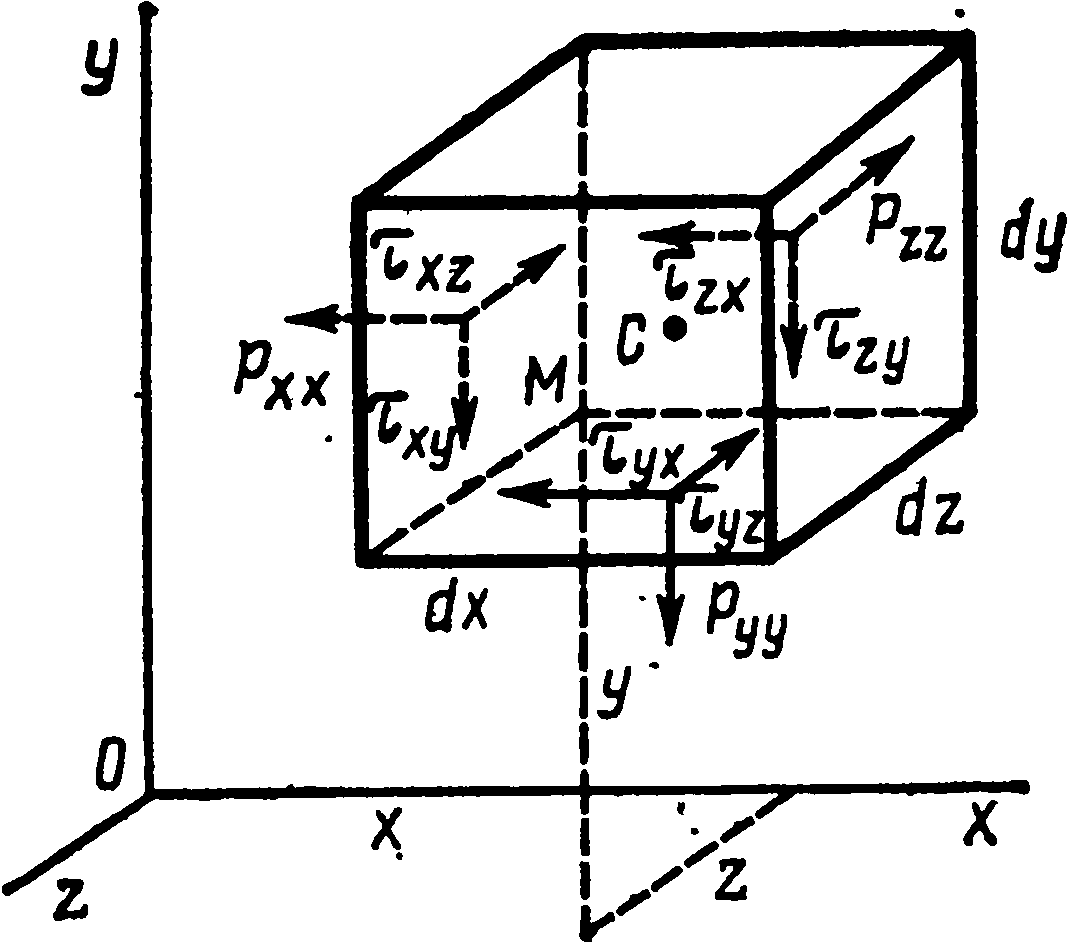
\includegraphics[width=0.3\linewidth]{img/surface-forces-on-viscous-fluid}
		\caption{Поверхностные силы, действующие на частицу вязкой жидкости.}
		\label{fig:3.3_surface-forces-on-viscous-fluid}
	\end{figure}
	Различие в поверхностных силах по сравнению с невязкой средой состоит в том, что в этом случае на грани частицы действуют не только нормальные напряжения, но и касательные, так как поверхностные силы в вязком газе не ортогональны к рассматриваемой поверхности. Это означает, что направление поверхностной силы, действующей на каждую грань параллелепипеда, не совпадает с нормалью к грани и, следовательно, каждая такая сила (напряжение) имеет три проекции на координатные оси.\n
	Введем следующие обозначения. Для каждой проекции вектора напряжения, действующего на рассматриваемую грань, примем два индекса: первый указывает направление нормали к рассматриваемой грани, а второй --- ось, на которую проецируется поверхностная сила (напряжение), действующая на эту грань. В этих обозначениях составляющие поверхностного напряжения, действующего на левую грань, перпендикулярную оси $x$, можно представить в виде $p_{xx}$, $\tau_{xy}$, $\tau_{xz}$; составляющие, действующие на грань, перпендикулярную оси $y$, --- в виде $\tau_{yx}$, $p_{yy}$, $\tau_{yz}$, а составляющие поверхностного напряжения, действующие на грань, перпендикулярную оси $z$, --- в виде $\tau_{zx}$, $\tau_{zy}$, $p_{zz}$, где $p_{xx}$, $p_{yy}$, $p_{zz}$ --- нормальные напряжения, действующие на грани рассматриваемого элементарного параллелепипеда; $\tau_{xy}$, $\tau_{xz}$, $\tau_{yx}$, $\tau_{yz}$, $\tau_{zx}$, $\tau_{zy}$ --- касательные напряжения.\n
	За положительные направления нормальных составляющих примем направления вдоль внешних нормалей к граням. На трех гранях, проходящих через точку $M$, за положительные направления касательных составляющих примем отрицательные направления осей координат, а на остальных трех гранях --- в сторону положительного направления координатных осей.\n
	Рассмотрим проекции на ось $x$ поверхностных сил, действующих на выделенную частицу газа. Проекции на ось $x$ дают нормальные напряжения, действующие на левую и правую грани:
	\begin{gather*}
		-p_{xx}\dd y\dd z; \quad \left[p_{xx} + \frac{\pp p_{xx}}{\pp x}\dd x\right]\dd x\dd y;
	\end{gather*}
	касательные напряжения, действующие на заднюю и переднюю грани:
	\begin{gather*}
		-\tau_{zx}\dd x\dd y; \quad \left[\tau_{zx} + \frac{\pp \tau_{zx}}{\pp z}\dd z\right]\dd x\dd y,
	\end{gather*}
	а также касательные напряжения, приложенные к нижней и верхней граням:
	\begin{gather*}
		-\tau_{yx}\dd x\dd z; \quad \left[\tau_{yx} + \frac{\pp \tau_{yx}}{\pp y}\dd y\right]\dd x\dd z.
	\end{gather*}\n
	Суммарная проекция на ось $x$ поверхностных сил, действующих на все грани параллелепипеда,
	\begin{gather*}
		\left(\frac{\pp p_{xx}}{\pp x} + \frac{\pp\tau_{yx}}{\pp y} + \frac{\pp\tau_{zx}}{\pp z}\right)\dd x\dd y\dd z.
	\end{gather*}\n
	Проекции массовых сил, отнесенных к единице массы, по-прежнему обозначим $X$, $Y$, $Z$. Тогда проекция на ось $x$ всех сил
	\begin{gather*}
		F_x = \left[X + \frac{1}{\rho}\left(\frac{\pp p_{xx}}{\pp x} + \frac{\pp\tau_{yx}}{\pp y} + \frac{\pp\tau_{zx}}{\pp z}\right)\right]\rho\dd x\dd y\dd z.
	\end{gather*}\n
	Используя принцип Даламбера, получаем:
	\begin{gather}
		-\frac{\dd v_x}{\dd t}\rho\dd x\dd y\dd z + \left[X + \frac{1}{\rho}\left(\frac{\pp p_{xx}}{\pp x} + \frac{\pp\tau_{yx}}{\pp y} + \frac{\pp\tau_{zx}}{\pp z}\right)\right]\rho\dd x\dd y\dd z = 0;\nonumber\\
		\frac{\dd v_x}{\dd t} = X + \frac{1}{\rho}\left(\frac{\pp p_{xx}}{\pp x} + \frac{\pp\tau_{yx}}{\pp y} + \frac{\pp\tau_{zx}}{\pp z}\right).\label{eq:314}
	\end{gather}\n
	Аналогично можно получить еще два уравнения:
	\begin{gather}
		\begin{dcases}\label{eq:315}
			\frac{\dd v_y}{\dd t} = Y + \frac{1}{\rho}\left(\frac{\pp \tau_{xy}}{\pp x} + \frac{\pp p_{yy}}{\pp y} + \frac{\pp\tau_{zy}}{\pp z}\right);\\
			\frac{\dd v_z}{\dd t} = Z + \frac{1}{\rho}\left(\frac{\pp \tau_{xz}}{\pp x} + \frac{\pp\tau_{yz}}{\pp y} + \frac{\pp p_{zz}}{\pp z}\right).
		\end{dcases}
	\end{gather}\n
	Покажем, что из шести касательных напряжений независимыми являются лишь три, причем $\tau_{xy} = \tau_{yx}$, $\tau_{yz} = \tau_{zy}$, $\tau_{xz} = \tau_{zx}$. Составим уравнения моментов, действующих на частицу сил, относительно осей, проходящих через центр частицы и параллельных осям координат. Моменты массовой силы и нормальных составляющих поверхностных сил относительно указанных осей равны нулю. Поэтому при составлении уравнений моментов необходимо учитывать только моменты от сил, определяемых касательными напряжениями. Например, уравнение моментов относительно оси, параллельной оси $z$, имеет вид
	\begin{gather*}
		-\tau_{yx}\frac{\dd x\dd z\dd y}{2} - \left[\tau_{yx} + \frac{\pp \tau_{yx}}{\pp y}\dd y\right]\frac{\dd x\dd z\dd y}{2} + \tau_{xy}\frac{\dd y\dd z\dd x}{2} + \left[\tau_{xy} + \frac{\pp \tau_{xy}}{\pp x}\dd x\right]\frac{\dd y\dd z\dd x}{2} = 0.
	\end{gather*}\n
	Отсюда, отбрасывая малые члены четвертого порядка, получаем $\tau_{xy} = \tau_{yx}$. Аналогично, из уравнений моментов относительно осей $x$ и $y$ имеем $\tau_{yz} = \tau_{zy}$, $\tau_{xz} = \tau_{zx}$. Система из трех уравнений \eqref{eq:314} и \eqref{eq:315} содержит шесть напряжений --- три нормальных $p_{xx}$, $p_{yy}$, $p_{zz}$ и три касательных $\tau_{xy} = \tau_{yx}$, $\tau_{yz} = \tau_{zy}$, $\tau_{xz} = \tau_{zx}$.\n
	Представим нормальные напряжения в следующем виде:
	\begin{gather}
		p_{xx} = -p + \pi_{xx}, \quad p_{yy} = -p + \pi_{yy}, \quad p_{zz} = -p + \pi_{zz},\label{eq:316}
	\end{gather}
	где $\pi_{xx}$, $\pi_{yy}$, $\pi_{zz}$ --- дополнительные нормальные напряжения, зависящие от вязкости. В невязкой среде и в покоящейся вязкой среде $\pi_{xx} = \pi_{yy} = \pi_{zz} = 0$.\n
	Воспользуемся гипотезой пропорциональности напряжений соответствующим скоростям деформационного движения. Согласно этой гипотезе, касательные напряжения пропорциональны скоростям деформации скашивания угла, а нормальные напряжения $\pi_{xx}$, $\pi_{yy}$, $\pi_{zz}$, зависящие от вязкости, пропорциональны соответствующим скоростям линейной деформации (в случае несжимаемой среды), скоростям линейной и объемной деформации (в случае сжимаемой среды):
	\begin{gather}
		\begin{dcases}\label{eq:317}
			\tau_{xy} = \tau_{yx} = \mu\left(\frac{\pp v_x}{\pp y} + \frac{\pp v_y}{\pp x}\right);\\
			\tau_{xz} = \tau_{zx} = \mu\left(\frac{\pp v_x}{\pp z} + \frac{\pp v_z}{\pp x}\right);\\
			\tau_{yz} = \tau_{zy} = \mu\left(\frac{\pp v_y}{\pp z} + \frac{\pp v_z}{\pp y}\right);
		\end{dcases}\\
		\begin{dcases}\label{eq:318}
			\pi_{xx} = 2\mu\frac{\pp v_x}{\pp x} + \tilde{\mu}\diverg{\vv{v}};\\
			\pi_{yy} = 2\mu\frac{\pp v_y}{\pp y} + \tilde{\mu}\diverg{\vv{v}};\\
			\pi_{zz} = 2\mu\frac{\pp v_z}{\pp z} + \tilde{\mu}\diverg{\vv{v}},
		\end{dcases}
	\end{gather}
	где $\mu$ --- динамическая вязкость, а $\tilde{\mu}$ --- величина, зависящая от коэффициента $\mu$.\n
	В частности, из уравнений \eqref{eq:317} можно получить известный закон Ньютона для одномерного течения жидкости параллельными слоями. Действительно, полагая, что жидкость движется вдоль оси $x$ $\left(v_y = v_z = 0\right)$, из первого выражения \eqref{eq:317} получаем $\tau_{xy} = \tau_{yx} = \mu\frac{\pp v_x}{\pp y}$ или $\tau = \mu\frac{\pp v}{\pp n}$, т. е. соотношения \eqref{eq:317} являются обобщением закона трения Ньютона.\n
	Из формул \eqref{eq:318} следует, что в общем случае $\pi_{xx} \ne \pi_{yy} \ne \pi_{zz}$, т. е. нормальные напряжения $p_{xx}$, $p_{yy}$, $p_{zz}$ по трем взаимноперпендикулярным площадкам, проведенным через точку $M$, различны. Примем за давление в данной точке вязкой среды величину
	\begin{gather}
		p = -\frac{1}{3}\left(p_{xx} + p_{yy} + p_{zz}\right).\label{eq:319}
	\end{gather}\n
	Подставляя в равенство \eqref{eq:319} выражения \eqref{eq:316} и \eqref{eq:318}, получаем, что в несжимаемой среде оно выполняется тождественно, так как при этом $\diverg\vv{v} = 0$, а для его выполнения в сжимаемой среде необходимо, чтобы
	\begin{gather}
		2\mu + 3\tilde{\mu} = 0, \quad \tilde{\mu} = -\frac{2}{3}\mu.\label{eq:320}
	\end{gather}\n
	В результате, используя \eqref{eq:316}, \eqref{eq:318} и \eqref{eq:320}, имеем
	\begin{gather}
		\begin{dcases}\label{eq:321}
			p_{xx} = -p + 2\mu\frac{\pp v_x}{\pp x} - \frac{2}{3}\mu\diverg\vv{v};\\
			p_{yy} = -p + 2\mu\frac{\pp v_y}{\pp y} - \frac{2}{3}\mu\diverg\vv{v};\\
			p_{zz} = -p + 2\mu\frac{\pp v_z}{\pp z} - \frac{2}{3}\mu\diverg\vv{v}.
		\end{dcases}
	\end{gather}\n
	Подставим выражения \eqref{eq:321} и \eqref{eq:317} в уравнения \eqref{eq:314} и \eqref{eq:315} и представим в них проекции полного ускорения $\frac{\dd v_x}{\dd t}$, $\frac{\dd v_y}{\dd t}$, $\frac{\dd v_z}{\dd t}$ в развернутом виде:
	\begin{gather*}
		\frac{\dd v_x}{\dd t} = \frac{\pp v_x}{\pp t} + v_x\frac{\pp v_x}{\pp x} + v_y\frac{\pp v_x}{\pp y} + v_z\frac{\pp v_x}{\pp z},\\
		\frac{\dd v_y}{\dd t} = \frac{\pp v_y}{\pp t} + v_x\frac{\pp v_y}{\pp x} + v_y\frac{\pp v_y}{\pp y} + v_z\frac{\pp v_y}{\pp z},\\
		\frac{\dd v_z}{\dd t} = \frac{\pp v_z}{\pp t} + v_x\frac{\pp v_z}{\pp x} + v_y\frac{\pp v_z}{\pp y} + v_z\frac{\pp v_z}{\pp z}.
	\end{gather*}\n
	Тогда получаем уравнения движения вязкой среды:
	\begin{gather}
		\begin{dcases}\label{eq:322}
			\begin{aligned}
				\rho\left(\frac{\pp v_x}{\pp t} + v_x\frac{\pp v_x}{\pp x} + v_y\frac{\pp v_x}{\pp y} + v_z\frac{\pp v_x}{\pp z}\right) &= \rho X - \frac{\pp p}{\pp x} +\\&+ \frac{\pp}{\pp x}\left[\mu\left(2\frac{\pp v_x}{\pp x} - \frac{2}{3}\diverg\vv{v}\right)\right] +\\&+ \frac{\pp}{\pp y}\left[\mu\left(\frac{\pp v_x}{\pp y} + \frac{\pp v_y}{\pp x}\right)\right] +\\&+ \frac{\pp}{\pp z}\left[\mu\left(\frac{\pp v_z}{\pp x} + \frac{\pp v_x}{\pp z}\right)\right];
			\end{aligned}\\
			\begin{aligned}
				\rho\left(\frac{\pp v_y}{\pp t} + v_x\frac{\pp v_y}{\pp x} + v_y\frac{\pp v_y}{\pp y} + v_z\frac{\pp v_y}{\pp z}\right) &= \rho Y - \frac{\pp p}{\pp y} +\\&+ \frac{\pp}{\pp y}\left[\mu\left(2\frac{\pp v_y}{\pp y} - \frac{2}{3}\diverg\vv{v}\right)\right] +\\&+ \frac{\pp}{\pp z}\left[\mu\left(\frac{\pp v_y}{\pp z} + \frac{\pp v_z}{\pp y}\right)\right] +\\&+ \frac{\pp}{\pp x}\left[\mu\left(\frac{\pp v_x}{\pp y} + \frac{\pp v_y}{\pp x}\right)\right];
			\end{aligned}\\
			\begin{aligned}
				\rho\left(\frac{\pp v_z}{\pp t} + v_x\frac{\pp v_z}{\pp x} + v_y\frac{\pp v_z}{\pp y} + v_z\frac{\pp v_z}{\pp z}\right) &= \rho Z - \frac{\pp p}{\pp z} +\\&+ \frac{\pp}{\pp z}\left[\mu\left(2\frac{\pp v_z}{\pp z} - \frac{2}{3}\diverg\vv{v}\right)\right] +\\&+ \frac{\pp}{\pp x}\left[\mu\left(\frac{\pp v_z}{\pp x} + \frac{\pp v_x}{\pp z}\right)\right] +\\&+ \frac{\pp}{\pp y}\left[\mu\left(\frac{\pp v_y}{\pp z} + \frac{\pp v_z}{\pp y}\right)\right].
			\end{aligned}
		\end{dcases}
	\end{gather}\n
	Дифференциальные уравнения \eqref{eq:322} называются \textit{уравнениями Навье-Стокса}. В этих уравнениях шесть неизвестных величин: $v_x$, $v_y$, $v_z$, $p$, $\rho$, $T$. Динамическая вязкость зависит от температуры. В уравнениях \eqref{eq:322} закон изменения $\mu$ в зависимости от температуры считается известным.\n
	Представим уравнения \eqref{eq:322}, предполагая, что коэффициент вязкости является постоянной величиной $\left(\mu = \mathrm{const}\right)$, в виде
	\begin{gather}
		\begin{dcases}\label{eq:323}
			\begin{aligned}
				\frac{\pp v_x}{\pp t} + v_x\frac{\pp v_x}{\pp x} + v_y\frac{\pp v_x}{\pp y} + v_z\frac{\pp v_x}{\pp z} = X - \frac{1}{\rho}\frac{\pp p}{\pp x} + \nu\Delta v_x + \frac{\nu}{3}\frac{\pp}{\pp x}\diverg\vv{v};
			\end{aligned}\\
			\begin{aligned}
				\frac{\pp v_y}{\pp t} + v_x\frac{\pp v_y}{\pp x} + v_y\frac{\pp v_y}{\pp y} + v_z\frac{\pp v_y}{\pp z} = Y - \frac{1}{\rho}\frac{\pp p}{\pp y} + \nu\Delta v_y + \frac{\nu}{3}\frac{\pp}{\pp y}\diverg\vv{v};
			\end{aligned}\\
			\begin{aligned}
				\frac{\pp v_z}{\pp t} + v_x\frac{\pp v_z}{\pp x} + v_y\frac{\pp v_z}{\pp y} + v_z\frac{\pp v_z}{\pp z} = Z - \frac{1}{\rho}\frac{\pp p}{\pp z} + \nu\Delta v_z + \frac{\nu}{3}\frac{\pp}{\pp z}\diverg\vv{v},
			\end{aligned}
		\end{dcases}
	\end{gather}
	где $\nu = \mu/\rho$ --- кинематическая вязкость.\n
	В векторной форме уравнения \eqref{eq:323} имеют вид
	\begin{gather}
		\frac{\dd\vv{v}}{\dd t} = \vv{f} - \frac{1}{\rho}\grad{p} + \nu\Delta\vv{v} + \frac{\nu}{3}\grad{\left(\diverg\vv{v}\right)}.\label{eq:324}
	\end{gather}\n
	Здесь $\Delta$ --- оператор Лапласа.\n
	В декартовых координатах
	\begin{gather*}
		\Delta\vv{v} = \frac{\pp^2\vv{v}}{\pp x^2} + \frac{\pp^2\vv{v}}{\pp y^2} + \frac{\pp^2\vv{v}}{\pp z^2}.
	\end{gather*}\n
	Уравнения \eqref{eq:324} по сравнению с уравнениями Эйлера \eqref{eq:313} имеют два дополнительных члена: первый из них учитывает влияние вязкости в несжимаемой среде, когда $\diverg\vv{v} = 0$, а второй --- дополнительное влияние вязкости с учетом сжимаемости (т. е. при $\diverg\vv{v} \ne 0$).
	
	\subsection{Полная система уравнений сплошной среды}
	Рассмотрим систему уравнений невязкого газа. В этом случае для несжимаемой среды неизвестными величинами являются три составляющие скорости $v_x$, $v_y$, $v_z$ и давление $p$, а полная система уравнений состоит из уравнений Эйлера и уравнения неразрывности:
	\begin{gather}
		\frac{\dd\vv{v}}{\dd t} = \vv{f} - \frac{1}{\rho}\grad p, \quad \diverg\vv{v} = 0.\label{eq:333}
	\end{gather}\n
	С учетом сжимаемости полная система уравнений должна включать шесть независимых уравнений для определения шести неизвестных величин --- составляющих скорости $v_x$, $v_y$, $v_z$, давления $p$, плотности $\rho$ и температуры $T$. К их числу относятся уравнения движения, неразрывности и уравнение состояния газа. В качестве шестого уравнения необходимо составить уравнение термодинамического процесса. Для изоэнтропических течений $s = c_v\ln p/\rho^k = \mathrm{const}$ зависимость между давлением и плотностью описывается уравнением $p/\rho^k = \mathrm{const}$. В дифференциальной форме это уравнение применительно к движению газа имеет вид
	\begin{gather*}
		\frac{\dd}{\dd t}\frac{p}{\rho^k} = 0;\\
		\frac{\pp}{\pp t}\frac{p}{\rho^k} + v_x\frac{\pp}{\pp x}\frac{p}{\rho^k} + v_y\frac{\pp}{\pp y}\frac{p}{\rho^k} + v_z\frac{\pp}{\pp z}\frac{p}{\rho^k} = 0
	\end{gather*}
	или
	\begin{gather}
		\frac{\pp}{\pp t}\frac{p}{\rho^k} + \vv{v}\grad\frac{p}{\rho^k} = 0.\label{eq:334}
	\end{gather}\n
	Используя уравнение \eqref{eq:334}, получаем полную систему уравнений для невязкого сжимаемого газа:
	\begin{gather}
		\begin{dcases}\label{eq:335}
			\frac{\dd\vv{v}}{\dd t} = \vv{f} - \frac{1}{\rho}\grad p,\\
			\frac{\pp\rho}{\pp t} + \diverg\left(\rho\vv{v}\right) = 0,\\
			p = R\rho T,\\
			\frac{\pp}{\pp t}\frac{p}{\rho^k} + \vv{v}\grad\frac{p}{\rho^k} = 0.
		\end{dcases}
	\end{gather}\n
	В случае вязкой несжимаемой среды полная система уравнений состоит из уравнения Навье-Стокса и уравнения неразрывности:
	\begin{gather}
		\begin{dcases}\label{eq:336}
			\frac{\dd\vv{v}}{\dd t} = \vv{f} - \frac{1}{\rho}\grad p + \nu\Delta\vv{v},\\
			\diverg\vv{v} = 0.
		\end{dcases}
	\end{gather}
	Здесь неизвестными являются составляющие скорости и давление.\n
	В общем случае вязкой сжимаемой среды необходимо использовать уравнение движения вязкого сжимаемого газа \eqref{eq:322}, уравнение неразрывности \eqref{eq:34}, уравнение энергии для вязкого теплопроводного газа\footnote{См. \cite{2}, \S3.5.} и уравнение состояния газа \eqref{eq:11}.
	
	\subsection{Начальные и граничные условия}
	Решения системы уравнений должны удовлетворять начальным и граничным условиям. Начальные условия необходимы при решении задачи для неустановившегося движения и определяют значения искомых функций в некоторый заданный момент времени.\n
	Граничные условия задаются при решении задачи как установившегося, так и неустановившегося движения газа и должны выполняться в каждый момент времени. В невозмущенном потоке $\vv{v} = \vv{v_\infty}$, $p = p_\infty$, $\rho = \rho_\infty$, $T = T_\infty$.\n
	При рассмотрении задачи обтекания тела потоком невязкого газа должно выполняться \underLine{условие безотрывности обтекания} (условие непротекания). Поскольку при этом вектор скорости потока направлен по касательной к поверхности, то нормальная составляющая скорости в каждой точке поверхности равна нулю: $\left(v_n\right)_S = 0$. Если поверхность задана уравнением $f\left(x,\; y,\; z\right) = 0$, то направление нормали к поверхности в любой точке совпадает с направлением вектора:
	\begin{gather*}
		\grad f = \vv{i}\frac{\pp f}{\pp x} + \vv{j}\frac{\pp f}{\pp y} + \vv{k}\frac{\pp f}{\pp z}.
	\end{gather*}
	На основании условия безотрывности обтекания векторы скорости $\vv{v}$ и $\grad f$ в каждой точке поверхности должны быть ортогональны, т. е. скалярное произведение этих векторов должно быть равным нулю. Тогда условие безотрывности обтекания $\left(v_n\right)_S = 0$ можно представить в следующем виде: $\left(\vv{v}\grad f\right) = 0$, или
	\begin{gather}
		v_x\frac{\pp f}{\pp x} + v_y\frac{\pp f}{\pp y} + v_z\frac{\pp f}{\pp z} = 0.\label{eq:337}
	\end{gather}\n
	Следовательно, в случае невязкого газа необходимо задать значение $v_x$, $v_y$, $v_z$, $p$, $\rho$, $T$ на бесконечности, а на поверхности задается одно условие --- равенство нулю линейной комбинации $v_x$, $v_y$, $v_z$ с переменными коэффициентами \eqref{eq:337}.\n
	При исследовании обтекания тела потоком вязкого газа на поверхности тела выполняются \underLine{граничные условия прилипания вязкой среды к поверхности}, т. е. условие равенства нулю скорости потока $v_S = 0$.\n
	Кроме того, на поверхности необходимо задать \underLine{граничные условия для температуры газа}. В зависимости от решаемой задачи эти условия могут быть сформулированы по-разному: а) задана температура поверхности тела $T_S = T_\mathrm{ст}$; б) в каждой точке поверхности и в любой момент времени может быть задан удельный тепловой поток $q$. Поскольку удельный тепловой поток, осуществляемый посредством теплопроводности, согласно закону Фурье, можно представить в виде $q = -\lambda\frac{\pp T}{\pp n}$, то в этом случае граничное условие эквивалентно заданным значениям производной температуры по нормали к поверхности тела, $\frac{\pp T}{\pp n}$. В случае теплоизолированной стенки $\frac{\pp T}{\pp n} = 0$; в) задана связь между неизвестными значениями $T_\mathrm{ст}$ и $\left(\frac{\pp T}{\pp n}\right)_S$:
	\begin{gather}
		\alpha\left(T_\mathrm{ст} - T_r\right) = -\lambda\frac{\pp T}{\pp n},\label{eq:338}
	\end{gather}
	где $\alpha$ --- коэффициент теплоотдачи, $\mathrm{\frac{Вт}{м^2 \cdot К}}$; $T_r$ --- температура восстановления, К.\n
	При малых скоростях значение $T_r$ близко к $T_\infty$, а при больших скоростях движения газа оно может быть значительно выше.\n
	Следует отметить, что в случае вязкого газа полная система дифференциальных уравнений имеет первый порядок относительно давления и плотности и второй порядок относительно составляющих скорости и температуры. Поэтому для определения давления и плотности по-прежнему достаточно задать одно условие (на бесконечности), а для нахождения $v_x$, $v_y$, $v_z$ и $T$ необходимы два условия --- на бесконечности и на поверхности тела.
	
	\subsection{Интегралы дифференциальных уравнений движения невязкого газа}
	Интегралы дифференциальных уравнений \eqref{eq:312'} могут быть получены в двух частных случаях --- для потенциального течения (уравнение Лагранжа) и для установившегося движения (уравнение Бернулли).
	
	\subsubsection{Уравнение Лагранжа}
	Рассмотрим случай неустановившегося потенциального движения газа. При этом $\vv{\omega} = \frac{\rot\vv{v}}{2} = 0$, $\omega_x = \omega_y = \omega_z = 0$. Отсюда $\frac{\pp v_y}{\pp z} = \frac{\pp v_z}{\pp y}$, $\frac{\pp v_x}{\pp z} = \frac{\pp v_z}{\pp x}$, $\frac{\pp v_y}{\pp x} = \frac{\pp v_x}{\pp y}$.\n
	Преобразуем левые части уравнений \eqref{eq:312'}. Используя условие потенциальности течения, получаем:
	\begin{gather*}
		\frac{\pp v_x}{\pp t} = \frac{\pp}{\pp t}\frac{\pp\varphi}{\pp x} = \frac{\pp}{\pp x}\frac{\pp\varphi}{\pp t};\\
		v_y\frac{\pp v_x}{\pp y} = v_y\frac{\pp v_y}{\pp x} = \frac{\pp}{\pp x}\frac{v_y^2}{2};\\
		v_z\frac{\pp v_x}{\pp z} = v_z\frac{\pp v_z}{\pp x} = \frac{\pp}{\pp x}\frac{v_z^2}{2}.
	\end{gather*}\n
	Тогда
	\begin{subequations}
		\begin{gather}
			\frac{\dd v_x}{\dd t} = \frac{\pp}{\pp x}\left(\frac{\pp\varphi}{\pp t} + \frac{v^2}{2}\right),\label{eq:339а}
		\end{gather}
		где $v^2 = v_x^2 + v_y^2 + v_z^2$.\n
		Аналогично,
		\begin{gather}\label{eq:339б}
			\begin{gathered}
				\frac{\dd v_y}{\dd t} = \frac{\pp}{\pp y}\left(\frac{\pp\varphi}{\pp t} + \frac{v^2}{2}\right);\\
				\frac{\dd v_z}{\dd t} = \frac{\pp}{\pp z}\left(\frac{\pp\varphi}{\pp t} + \frac{v^2}{2}\right).
			\end{gathered}
		\end{gather}\n
	\end{subequations}
	Для того чтобы преобразовать правые части уравнений \eqref{eq:312'}, введем функцию давления $P$, определяемую из соотношения $\frac{\dd p}{\rho} = \dd P$ или $\int\frac{\dd p}{\rho} = P$. Тогда
	\begin{gather}\label{eq:340}
		\frac{1}{\rho}\frac{\pp p}{\pp x} = \frac{\pp P}{\pp x};\quad
		\frac{1}{\rho}\frac{\pp p}{\pp y} = \frac{\pp P}{\pp y};\quad
		\frac{1}{\rho}\frac{\pp p}{\pp z} = \frac{\pp P}{\pp z}.
	\end{gather}\n
	Если известна однозначная зависимость между давлением и плотностью $p\left(\rho\right)$, функцию давления определить легко.\n
	Кроме того, примем, что массовые силы обладают потенциалом. Обозначим потенциал единичной массовой силы $U$. При этом
	\begin{gather}\label{eq:341}
		X = \frac{\pp U}{\pp x},\quad
		Y = \frac{\pp U}{\pp y},\quad
		Z = \frac{\pp U}{\pp z}.
	\end{gather}\n
	Для силы тяжести $U = -gy$.\n
	Подставляя выражения \eqref{eq:339а}, \eqref{eq:339б} -- \eqref{eq:341} в систему уравнений \eqref{eq:312'}, получаем:
	\begin{gather*}
		\frac{\pp}{\pp x}\left(\frac{\pp\varphi}{\pp t} + \frac{v^2}{2} + \int\frac{\dd p}{\rho} - U\right) = 0;\\
		\frac{\pp}{\pp y}\left(\frac{\pp\varphi}{\pp t} + \frac{v^2}{2} + \int\frac{\dd p}{\rho} - U\right) = 0;\\
		\frac{\pp}{\pp z}\left(\frac{\pp\varphi}{\pp t} + \frac{v^2}{2} + \int\frac{\dd p}{\rho} - U\right) = 0.
	\end{gather*}\n
	Отсюда следует, что выражение $\frac{\pp\varphi}{\pp t} + \frac{v^2}{2} + \int\frac{\dd p}{\rho}$ не зависит от координат, т. е. имеет одинаковые значения для любых точек потенциального потока. В случае неустановившегося движения оно является функцией только времени:
	\begin{gather}\label{eq:342}
		\frac{\pp\varphi}{\pp t} + \frac{v^2}{2} + \int\frac{\dd p}{\rho} - U = C\left(t\right).
	\end{gather}\n
	Уравнение \eqref{eq:342} называется \textit{уравнением Лагранжа}.\n
	В случае установившегося потенциального течения $\frac{\pp\varphi}{\pp t} = 0$ величина $C$ не зависит от времени. Тогда интеграл \eqref{eq:342} приобретет вид
	\begin{gather}\label{eq:343}
		\frac{v^2}{2} + \int\frac{\dd p}{\rho} - U = \mathrm{const}.
	\end{gather}\n
	Интеграл \eqref{eq:343} называется \textit{уравнением Лагранжа-Бернулли}.
	
	\subsubsection{Уравнение Бернулли}
	Рассмотрим установившееся движение газа. При этом $\frac{\pp v_x}{\pp t} = \frac{\pp v_y}{\pp t} = \frac{\pp v_z}{\pp t} = 0$, $p = p\left(x,\; y,\; z\right)$. Преобразуем левую часть первого уравнения системы уравнений \eqref{eq:312}:
	\begin{gather*}
		\begin{aligned}
			\frac{\dd v_x}{\dd t} &= v_x\frac{\pp v_x}{\pp x} + v_y\frac{\pp v_x}{\pp y} + v_z\frac{\pp v_x}{\pp z} =\\
			&= \frac{\pp}{\pp x}\left(\frac{v_x^2}{2}\right) + \frac{\pp}{\pp x}\left(\frac{v_y^2}{2}\right) + v_y\left(\frac{\pp v_x}{\pp y} - \frac{\pp v_y}{\pp x}\right) + \frac{\pp}{\pp x}\left(\frac{v_z^2}{2}\right) + v_z\left(\frac{\pp v_x}{\pp z} - \frac{\pp v_z}{\pp x}\right);
		\end{aligned}\\
		\frac{\dd v_x}{\dd t} = \frac{\pp}{\pp x}\left(\frac{v^2}{2}\right) + 2\left(v_z\omega_y - v_y\omega_z\right),
	\end{gather*}
	где выражение $\left(v_z\omega_y - v_y\omega_z\right)$ --- проекция вектора $\left[\vv{\omega}\vv{v}\right]$ на направление оси $x$.\n
	Тогда
	\begin{gather}\label{eq:344}
		\frac{\dd v_x}{\dd t} = \frac{\pp}{\pp x}\frac{v^2}{2} + 2\left[\vv{\omega}\vv{v}\right]_x.
	\end{gather}\n
	Аналогично для производных $\frac{\dd v_y}{\dd t}$ и $\frac{\dd v_z}{\dd t}$
	\begin{gather}\label{eq:345}
		\frac{\dd v_y}{\dd t} = \frac{\pp}{\pp y}\frac{v^2}{2} + \left[\vv{\omega}\vv{v}\right]_y;\quad
		\frac{\dd v_z}{\dd t} = \frac{\pp}{\pp z}\frac{v^2}{2} + \left[\vv{\omega}\vv{v}\right]_z.
	\end{gather}\n
	Здесь $\left[\vv{\omega}\vv{v}\right]_x$, $\left[\vv{\omega}\vv{v}\right]_y$, $\left[\vv{\omega}\vv{v}\right]_z$ --- проекции вектора $\left[\vv{\omega}\vv{v}\right]$ по осям координат.\n
	Подставим выражения \eqref{eq:344} и \eqref{eq:345} в уравнения \eqref{eq:312}. Кроме того, введем функцию давления \eqref{eq:340} и потенциал единичной массовой силы $U$ \eqref{eq:341}. Тогда
	\begin{gather*}
		\frac{\pp}{\pp x}\left(\frac{v^2}{2} + \int\frac{\dd p}{\rho} - U\right) = -2\left[\vv{\omega}\vv{v}\right]_x;\\
		\frac{\pp}{\pp y}\left(\frac{v^2}{2} + \int\frac{\dd p}{\rho} - U\right) = -2\left[\vv{\omega}\vv{v}\right]_y;\\
		\frac{\pp}{\pp z}\left(\frac{v^2}{2} + \int\frac{\dd p}{\rho} - U\right) = -2\left[\vv{\omega}\vv{v}\right]_z.
	\end{gather*}\n
	Умножим первое уравнение на $\dd x$, второе --- на $\dd y$, третье --- на $\dd z$ и почленно сложим. В результате для установившегося движения
	\begin{gather*}
		\dd\left(\frac{v^2}{2} + \int\frac{\dd p}{\rho} - U\right) = -2\left(\left[\vv{\omega}\vv{v}\right]\vv{\dd s}\right),
	\end{gather*}
	где $\vv{\dd s}$ --- вектор элементарной дуги с проекциями $\dd x$, $\dd y$, $\dd z$.\n
	Скалярное произведение $\left(\left[\vv{\omega}\vv{v}\right]\vv{\dd s}\right) = 0$ вдоль линии тока и вдоль вихревой линии, так как векторы $\left[\vv{\omega}\vv{v}\right]$ и $\vv{\dd s}$ перпендикулярны. Таким образом, вдоль линий тока и вихревых линий
	\begin{gather}\label{eq:346}
		\dd\left(\frac{v^2}{2} + \int\frac{\dd p}{\rho} - U\right) = 0;\quad
		\frac{v^2}{2} + \int\frac{\dd p}{\rho} - U = \mathrm{const},
	\end{gather}
	где значение постоянной различно для разных линий тока и вихревых линий.\n
	Уравнение \eqref{eq:346} называется \textit{уравнением или интегралом Бернулли}. Это уравнение имеет фундаментальное значение в теории движения невязких жидкостей и газов и является теоретической основой для практических расчетов.\n
	Рассмотрим уравнения Бернулли для различных частных случаев движения жидкости и газа.
	\paragraph{Несжимаемая среда.} Для несжимаемой среды $\left(\rho = \mathrm{const}\right)$ функция давления равна $P = p/\rho$. Примем $U = -gy$. Тогда уравнение \eqref{eq:346} приобретет вид
	\begin{gather}\label{eq:347}
		\frac{v^2}{2} + \frac{p}{\rho} + gy = \mathrm{const}.
	\end{gather}\n
	Если пренебречь массовыми силами, то \eqref{eq:347} примет вид
	\begin{gather}\label{eq:348}
		p + \frac{\rho v^2}{2} = \mathrm{const}.
	\end{gather}\n
	Из уравнения \eqref{eq:348} следует, что при установившемся движении несжимаемой среды полное давление, равное $p + \frac{\rho v^2}{2}$, вдоль линии тока или вихревой линии остается неизменным.
	\paragraph{Сжимаемая среда без учета массовых сил.} Для сжимаемого газа без учета массовых сил
	\begin{gather}\label{eq:349}
		\frac{v^2}{2} + \int\frac{\dd p}{\rho} = \mathrm{const}.
	\end{gather}
	\paragraph{Изоэнтропическое течение.} Допустим, что течение газа является изэнтропическим. Тогда $p/\rho^k = C$. Отсюда
	\begin{gather*}
		\dd p = C k\rho^{k-1}\dd\rho \quad \mathrm{и} \quad \frac{\dd p}{\rho} = C k\rho^{k-2}\dd\rho,\\
		\int\frac{\dd p}{\rho} = C\frac{k}{k-1}\rho^{k-1} = \frac{k}{k-1}\frac{p}{\rho}.
	\end{gather*}\n
	Подставляя выражение интеграла в \eqref{eq:349}, получаем:
	\begin{gather}
		\frac{v^2}{2} + \frac{k}{k-1}\frac{p}{\rho} = \mathrm{const};\label{eq:350}\\
		\frac{v^2}{2} + \frac{k}{k-1}RT = \mathrm{const}.\label{eq:351}
	\end{gather}\n
	Учитывая, что $\frac{k}{k-1}\frac{p}{\rho} = \frac{k}{k-1}RT = i$, имеем
	\begin{gather}\label{eq:352}
		\frac{v^2}{2} + i = \mathrm{const}.
	\end{gather}\n
	Уравнение Бернулли в форме \eqref{eq:352} совпадает с уравнением энергии для невязкого и нетеплопроводного газа\footnote{См. \cite{2}, \S3.5.}.
	\paragraph{Ошибка в определении давления при использовании уравнения Бернулли, полученного без учета сжимаемости.} Выясним, какова ошибка в определении давления при использовании уравнения Бернулли \eqref{eq:348}, полученного без учета сжимаемости. Допустим, что поток воздуха обтекает какое-либо тело. Пусть на достаточно большом удалении от тела скорость потока $v_\infty$ и давление $p_\infty$. В критической точке на поверхности скорость равна нулю, а давление равно давлению торможения $p_0$. Используем уравнение Бернулли для несжимаемой среды \eqref{eq:348}. Постоянную $C$ определим из условий на бесконечности:
	\begin{gather*}
		C = p_\infty + \frac{\rho v_\infty^2}{2}.
	\end{gather*}\n
	Подставляя найденное значение в уравнение \eqref{eq:348}, находим
	\begin{gather*}
		p = p_\infty + \frac{\rho v_\infty^2}{2} - \frac{\rho v^2}{2}.
	\end{gather*}\n
	Для определения давления в критической точке положим $v = 0$. В результате
	\begin{gather}\label{eq:353}
		p_0 = p_\infty + \frac{\rho v_\infty^2}{2}.
	\end{gather}\n
	Определим теперь давление в критической точке с учетом сжимаемости. Для этого найдем постоянную $C$ в уравнении \eqref{eq:350} из условий на бесконечности:
	\begin{gather*}
		C = \frac{k}{k-1}\frac{p_\infty}{\rho_\infty} + \frac{v_\infty^2}{2}.
	\end{gather*}\n
	Подставляя найденное значение $C$ в уравнение \eqref{eq:350} и используя выражение $p/\rho^k = p_\infty/\rho_\infty^k$, получаем
	\begin{gather*}
		\frac{k}{k-1}\frac{p_\infty}{\rho_\infty}\left(\frac{p}{p_\infty}\right)^{\frac{k-1}{k}} + \frac{v^2}{2}= \frac{k}{k-1}\frac{p_\infty}{\rho_\infty} + \frac{v_\infty^2}{2}.
	\end{gather*}\n
	Положив в этом уравнении $v = 0$, что соответствует критической точке, будем иметь
	\begin{gather*}
		\frac{k}{k-1}\frac{p_\infty}{\rho_\infty}\left(\frac{p_0}{p_\infty}\right)^{\frac{k-1}{k}} = \frac{k}{k-1}\frac{p_\infty}{\rho_\infty} + \frac{v_\infty^2}{2}
	\end{gather*}
	или, учитывая, что $k\frac{p_\infty}{\rho_\infty} = a_\infty^2$, $v_\infty/a_\infty = \mathrm{M_\infty}$, после несложных преобразований получаем
	\begin{gather}\label{eq:354}
		\frac{p_0}{p_\infty} = \left(1 + \frac{k-1}{2}\mathrm{M_\infty^2}\right)^{\frac{k}{k-1}}.
	\end{gather}\n
	Формулой \eqref{eq:354} можно пользоваться для определения давления в критической точке $p_0$ с учетом сжимаемости.\n
	Поскольку влиянием сжимаемости потока можно пренебречь только при малых значениях числа $\mathrm{M_\infty}$, то, для того чтобы выяснить пределы применимости формулы \eqref{eq:353}, полученной без учета сжимаемости, в формуле \eqref{eq:354} примем $\mathrm{M_\infty}\ll 1$. При этом условии разложим правую часть выражения \eqref{eq:354} в ряд по степеням $\frac{k-1}{2}\mathrm{M_\infty^2}\ll 1$ по формуле бинома Ньютона:
	\begin{gather*}
		\frac{p_0}{p_\infty} = 1 + \frac{k}{k-1}\frac{k-1}{2}\M_\infty^2 + \frac{1}{2}\frac{k}{k-1}\left(\frac{k}{k-1} - 1\right)\left(\frac{k-1}{2}\M_\infty^2\right)^2 +\\+ \frac{1}{6}\frac{k}{k-1}\left(\frac{k}{k-1} - 1\right)\left(\frac{k}{k-1} - 2\right)\left(\frac{k-1}{2}\M_\infty^2\right)^3 + \dots,
	\end{gather*}
	или
	\begin{gather*}
		\frac{p_0}{p_\infty} = 1 + \frac{k}{2}\M_\infty^2\left(1 + \frac{\M_\infty^2}{4} + \frac{2-k}{24}\M_\infty^4 + \dots\right).
	\end{gather*}\n
	Отсюда, учитывая, что $\frac{k}{2}p_\infty\M_\infty^2 = \frac{\rho_\infty v_\infty^2}{2}$, имеем
	\begin{gather*}
		p_0 = p_\infty + \frac{\rho_\infty v_\infty^2}{2}\left(1 + \frac{\M_\infty^2}{4} + \frac{2-k}{24}\M_\infty^4 + \dots\right).
	\end{gather*}\n
	Представим это выражение в виде
	\begin{gather}\label{eq:355}
		p_0 = p_\infty + \frac{\rho_\infty v_\infty^2}{2}\left(1 + \varepsilon_\mathrm{p}\right),
	\end{gather}
	где
	\begin{gather}\label{eq:356}
		\varepsilon_\mathrm{p} = 1 + \frac{\M_\infty^2}{4} + \frac{2-k}{24}\M_\infty^4 + \dots
	\end{gather}\n
	Сравнивая формулы \eqref{eq:355} и \eqref{eq:353}, замечаем, что величина $\varepsilon_\mathrm{p}$ в формуле \eqref{eq:355} представляет собой погрешность, отнесенную к скоростному напору при определении давления в критической точке без учета сжимаемости. Величину $\varepsilon_\mathrm{p}$ можно трактовать также как относительную поправку, учитывающую влияние сжимаемости. Из формулы \eqref{eq:356} следует, что величина $\varepsilon_\mathrm{p}$ зависит от числа $\M_\infty$.\n
	Ниже приведены значения $\varepsilon_\mathrm{p}$ в зависимости от $\M_\infty$ при $k = 1,4$:
	\begin{table}[htbp]
		\centering
		\begin{tabular}{c|cccccc}
			$\M$ & 0,1 & 0,2 & 0,3 & 0,4 & 0,5 & 0,6 \\
			\hline
			$\varepsilon_\mathrm{p}$ & 0,25 & 1,0 & 2,25 & 4,0 & 6,2 & 9,0 \\
		\end{tabular}
	\end{table}\n
	Отсюда следует, что, допуская ошибку не более 2\%, при определении давления $p_0$ можно пользоваться уравнением Бернулли, полученным без учета сжимаемости воздуха при $\M < 0,3$. При больших скоростях $\left(\M > 0,3\right)$ ошибка в определении $p_0$ возрастает.
	
	\newpage
	\part{Профиль и крыло конечного размаха в несжимаемом потоке}
	
	\section{Лекция 5}
	
	\subsection{Геометрические характеристики}
	
	Обычно форму крыла определяют, задавая профиль, вид сверху, угол крутки и угол поперечного $V$.\n
	\begin{figure}[htbp]
		\centering
		\begin{minipage}{0.49\textwidth}
			\centering
			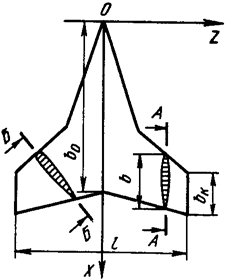
\includegraphics[width=0.5\textwidth]{img/wing-geometric-characteristics}
			\captionof{figure}{Определение геометрических характеристик крыла.}
			\label{fig:wing-geometric-characteristics}
		\end{minipage}
		\hfill
		\begin{minipage}{0.49\textwidth}
			\centering
			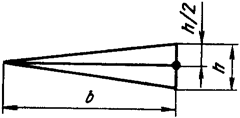
\includegraphics[width=0.5\textwidth]{img/profile-chord-cut-off-aft-part}
			\captionof{figure}{Хорда профиля со срезанной кормовой частью.}
			\label{fig:profile-chord-cut-off-aft-part}
		\end{minipage}
	\end{figure}
	\textit{Профилем крыла} называют местное сечение крыла плоскостью, параллельной базовой плоскости самолета. В случае изолированного крыла --- плоскостью, параллельной его плоскости симметрии (\cref{fig:wing-geometric-characteristics}, сечение А-А). Иногда под профилем понимают сечение крыла плоскостью, перпендикулярной передней (\cref{fig:wing-geometric-characteristics}, сечение Б-Б) или задней кромке, или какой-либо другой линии.\n
	Отрезок прямой, соединяющей наиболее удаленные точки контура профиля, называют \textit{хордой профиля} и обозначают $b$. В случае симметричного профиля со срезанной кормовой частью, например клиновидного (\cref{fig:profile-chord-cut-off-aft-part}), хордой считают отрезок прямой, соединяющей точку, лежащую на середине кормового среза, и наиболее удаленную от нее точку контура профиля.\n
	Геометрическим местом передних точек хорд профилей является \textit{передняя кромка крыла}, а геометрическим местом задних точек --- \textit{задняя кромка}.\n
	Отрезок прямой, соединяющий точки пересечения передней и задней кромок крыла плоскостью, содержащей профиль крыла, называют \textit{местной хордой крыла} и обозначают $b\left(z\right)$. Очевидно, что местная хорда крыла --- это хорда профиля в рассматриваемом сечении крыла.\n
	\begin{figure}[htbp]
		\centering
		\begin{minipage}{0.49\textwidth}
			\centering
			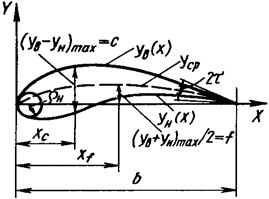
\includegraphics[width=0.6\textwidth]{img/profile-geometric-parameters}
			\captionof{figure}{Геометрические параметры профиля.}
			\label{fig:profile-geometric-parameters}
		\end{minipage}
		\hfill
		\begin{minipage}{0.49\textwidth}
			\centering
			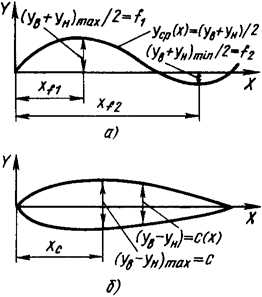
\includegraphics[width=0.7\textwidth]{img/profile-building}
			\captionof{figure}{Построение профиля по средней линии (\textit{а}) и распределению толщин (\textit{б}).}
			\label{fig:profile-building}
		\end{minipage}
	\end{figure}
	Описывая форму профиля, применяют прямоугольную систему координат $OXY$ с началом в передней точке хорды. Ось $OX$ направляют по хорде от передней точки к задней, а ось $OY$ --- вверх. Контур профиля задают с помощью таблицы или аналитически. Формы верхней и нижней частей контура задают отдельно: $y_\mathrm{в} = y_\mathrm{в}\left(x\right)$; $y_\mathrm{н} = y_\mathrm{н}\left(x\right)$ (\cref{fig:profile-geometric-parameters}). Контур профиля можно строить также, задавая среднюю линию $y_\mathrm{ср}\left(x\right) = \frac{1}{2}\left(y_\mathrm{в} + y_\mathrm{н}\right)$ и распределение толщин $y_\mathrm{в} - y_\mathrm{н} = c\left(x\right)$ (\cref{fig:profile-building}).\n
	\underLine{Основными геометрическими характеристиками профиля являются} (см. \cref{fig:profile-geometric-parameters}; \cref{fig:profile-building}):\n
	\begin{enumerate}
		\item относительная толщина $\bar{c} = \left(y_\mathrm{в} - y_\mathrm{н}\right)_\mathrm{max}/b$;
		\item 	относительная координата сечения, в котором профиль имеет максимальную толщину $\bar{x}_c = x_c/b$;
		\item 	относительная максимальная вогнутость, называемая обычно просто относительной вогнутостью, $\bar{f} = \left(y_\mathrm{в} + y_\mathrm{н}\right)_\mathrm{max}/\left(2b\right) > 0$ --- если средняя линия лежит выше хорды, $\bar{f} = \left(y_\mathrm{в} + y_\mathrm{н}\right)_\mathrm{min}/\left(2b\right) < 0$ --- если средняя линия проходит ниже хорды, $\bar{f} = 0$ --- в случае симметричного профиля;
		\item 	относительная координата сечения, в котором вогнутость максимальная, $\bar{x}_f = x_f/b$ (в случае $S$-образного профиля (см. \cref{fig:profile-building}) вогнутость характеризуется четырьмя величинами: $\bar{f}_1 = \left(y_\mathrm{в} + y_\mathrm{н}\right)_\mathrm{max}/\left(2b\right) > 0$; $\bar{f}_2 = \left(y_\mathrm{в} + y_\mathrm{н}\right)_\mathrm{min}/\left(2b\right) < 0$; $\bar{x}_{f1} = x_{f1}/b$; $\bar{x}_{f2} = x_{f2}/b$.
		\item 	относительный радиус носка $\bar{\rho}_\mathrm{н} = \rho_\mathrm{н}/b$;
		\item 	угол заострения профиля у задней кромки $2\tau$.
	\end{enumerate}
	Перечисленные характеристики --- безразмерные величины или выражаются в \% длины хорды.\n
	В некоторых случаях форму профиля у передней кромки характеризуют параметром заострения его носка: $\Delta y/b = \left(y_{6\%} - y_{0,15\%}\right)/b \cdot 100\%$, где $y_{6\%}$; $y_{0,15\%}$ --- измеренные по нормали к средней линии расстояния между контуром профиля и его средней линией в сечениях, удаленных от носка соответственно на 6\% и 0,15\% длины хорды.\n
	\begin{figure}[htbp]
		\centering
		\begin{minipage}{0.29\textwidth}
			\centering
			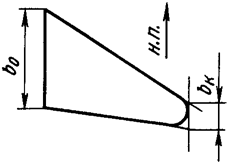
\includegraphics[width=0.9\textwidth]{img/wing-tip-chord-with-rounded-tips}
			\captionof{figure}{Концевая хорда крыла с закругленными концами.}
			\label{fig:wing-tip-chord-with-rounded-tips}
		\end{minipage}
		\hfill
		\begin{minipage}{0.69\textwidth}
			\centering
			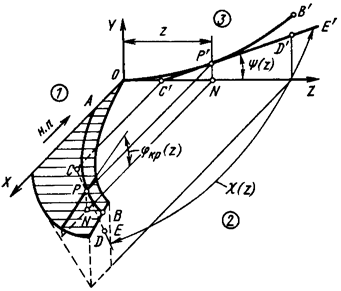
\includegraphics[width=0.7\textwidth]{img/determination-of-local-sweep-angles}
			\captionof{figure}{Определение местных углов стреловидности $\chi\left(z\right)$, поперечного $V$ крыла $\psi\left(z\right)$ и крутки $\varphi\left(z\right)$:\\\small{\textit{1} --- плоскость симметрии; \textit{2} --- базовая плоскость крыла, \textit{3} --- плоскость, перпендикулярная центральной хорде; $APB$ --- линия $1/4$ хорд; $CPDE$ --- касательная к линии $1/4$ хорд, $OP'B'$ --- проекция линии $1/4$ хорд на плоскость \textit{3}, $C'P'D'E'$ - проекция касательной к линии $1/4$ хорд на плоскость \textit{3}.}}
			\label{fig:determination-of-local-sweep-angles}
		\end{minipage}
	\end{figure}
	\underLine{Описывая форму крыла, используют следующие понятия и характеристики:}
	\begin{enumerate}
		\item размах крыла $l$ --- расстояние между двумя плоскостями, параллельными плоскости симметрии и касающимися концов крыла (см. \cref{fig:wing-geometric-characteristics});
		\item местная хорда $b\left(z\right)$ --- хорда профиля в сечении $z$;
		\item центральная хорда $b_0$ --- местная хорда в плоскости симметрии;
		\item концевая хорда $b_\mathrm{к}$ --- хорда в концевом сечении; если концы крыла закруглены, то $b_\mathrm{к}$ определяют в соответствии с \cref{fig:wing-tip-chord-with-rounded-tips};
		\item базовая плоскость крыла --- плоскость, содержащая центральную хорду и перпендикулярная плоскости симметрии;
		\item площадь крыла $S$ --- площадь проекции крыла на его базовую плоскость;
		\item средняя геометрическая хорда $b_\mathrm{ср} = S/b$;
		\item точка $n$ процентов хорды --- точка местной хорды, находящаяся на расстоянии $n$ процентов длины хорды от ее передней точки;
		\item линия $n$ процентов хорд --- линия, содержащая точки $n$ процентов хорд;
		\item местный угол стреловидности $\chi\left(z\right)$ --- угол между касательной к линии $1/4$ хорд в данном сечении и плоскостью \textit{3}, перпендикулярной центральной хорде (\cref{fig:determination-of-local-sweep-angles}); местный угол стреловидности по линии $n$ процентов хорд обозначают $\chi_n$, по передней кромке --- $\chi_\mathrm{п.к}$, по задней --- $\chi_\mathrm{з.к}$; $\chi\left(z\right) > 0$, если точка пересечения касательной $CPD$ с плоскостью симметрии находится впереди точки $P$;
		\item местный угол крутки крыла $\varphi_\mathrm{кр}\left(z\right)$ --- угол между хордой и базовой плоскостью крыла $2$ (см. \cref{fig:determination-of-local-sweep-angles}); $\varphi_\mathrm{кр}\left(z\right) > 0$, если координата $y$ передней точки хорды больше, чем задней;
		\item местный угол поперечного $V$ крыла $\psi\left(z\right)$ --- угол между проекцией на плоскость \textit{3}, перпендикулярную центральной хорде, касательной к линии $1/4$ хорд и базовой плоскостью крыла \textit{2} (см. \cref{fig:determination-of-local-sweep-angles}); $\psi\left(z\right) > 0$, если точка $P$ располагается выше точки пересечения касательной $CPD$ с базовой плоскостью крыла (точки $C$ на \cref{fig:determination-of-local-sweep-angles}).
	\end{enumerate}
	Если хорды всех сечений полукрыла лежат в одной плоскости, то $\varphi_\mathrm{кр}\left(z\right) = 0$, a $\psi\left(z\right) = \mathrm{const}$.\n
	\begin{figure}[htbp]
		\centering
		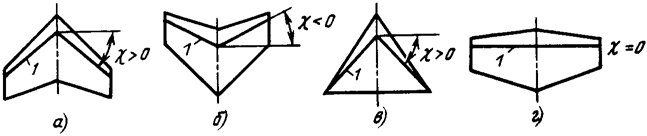
\includegraphics[width=0.75\linewidth]{img/trapezoidal-wings}
		\caption{Трапециевидные крылья:\\\small{\textit{а} --- стреловидное; \textit{б} --- обратной стреловидности; \textit{в} --- треугольное; \textit{г} --- нестреловидное; \textit{1} --- линия $1/4$ хорд.}}
		\label{fig:trapezoidal-wings}
	\end{figure}
	Форма трапециевидных крыльев на виде сверху однозначно определяется тремя параметрами: удлинением $\lambda = l^2/S$, сужением $\eta = b_0/b_\mathrm{к}$, углом стреловидности по линии $1/4$ хорд $\chi$ (или другой линии $\chi_n$). На \cref{fig:trapezoidal-wings} изображены трапециевидные крылья различной формы.\n
	Углы стреловидности трапециевидных крыльев по различным линиям связаны следующими соотношениями:
	\begin{gather}\label{eq:3.1}
		\begin{gathered}
			\tg\chi_n = \tg\chi - \frac{4n - 1}{\lambda}\frac{\eta - 1}{\eta + 1};\\
			\tg\chi_n = \tg\chi_\mathrm{п.к} - \frac{4n}{\lambda}\frac{\eta - 1}{\eta + 1},
		\end{gathered}
	\end{gather}
	где $n$ --- расстояние между точкой $n$ процентов хорды и ее передней точкой, выраженное в долях хорды, ($0 \leqslant n \leqslant 1$; $n = 0$ --- для передней кромки, $n = 1$ --- для задней). В случае треугольных крыльев имеют место следующие равенства:
	\begin{gather}\label{eq:3.2}
		\lambda\tg\chi_\mathrm{п.к} = 4;\quad
		\lambda\tg\chi = 3;\quad
		\lambda\tg\chi_{0,5} = 2;\quad
		\lambda\tg\chi_{0,75} = 1.
	\end{gather}\n
	\begin{figure}[htbp]
		\centering
		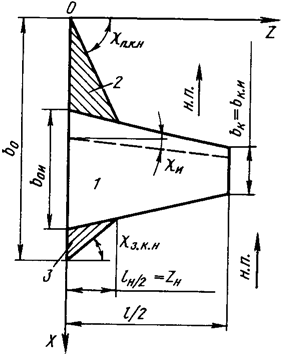
\includegraphics[width=0.35\linewidth]{img/wing-with-bulges}
		\caption{Определение формы крыла с наплывами:\\\small{$\chi_\mathrm{п.к.н}$, $\chi_\mathrm{з.к.н}$ --- углы стреловидности передней и задней кромок наплыва, $\chi_\mathrm{и}$ --- угол стреловидности исходного крыла, $b_\mathrm{0\,и}$, $b_\mathrm{к\,и}$ --- центральная и концевая хорды исходного крыла.}}
		\label{fig:wing-with-bulges}
	\end{figure}
	В последнее время широкое распространение получили крылья с наплывами (\cref{fig:wing-with-bulges}). Применяют крылья, имеющие передние наплывы \textit{2}, и крылья, имеющие передние и задние наплывы \textit{2} и \textit{3}. Кромки наплывов делают прямолинейными и криволинейными.\n
	Начальное крыло \textit{1}, на основе которого строят крыло с наплывом, называют исходным, или базовым.\n
	Описывая геометрию крыльев сложной формы на виде сверху, приходится применять больше трех параметров, а иногда и аналитические зависимости.\n
	При расчете продольной статической устойчивости и положения фокуса по углу атаки используют \textit{среднюю аэродинамическую хорду}. Ее длину обозначают $b_\mathrm{A}$. Относя расстояние между фокусом по углу атаки и центром масс к $b_\mathrm{A}$, получают универсальную характеристику продольной статической устойчивости.\n
	Координата фокуса, рассчитанная относительно носка САХ и отнесенная к длине САХ, является весьма стабильной, и ею целесообразно пользоваться при сравнении положений фокусов крыльев различной формы.\n
	Координаты носка и длина САХ определяются следующими соотношениями:
	\begin{gather}\label{eq:3.3}
		x_\mathrm{A} = \frac{1}{S}\int\limits_{-l/2}^{+l/2}b'\left(z\right)x\dd z;\quad
		y_\mathrm{A} = \frac{1}{S}\int\limits_{-l/2}^{+l/2}b'\left(z\right)y\dd z;\quad
		b_\mathrm{A} = \frac{1}{S}\int\limits_{-l/2}^{+l/2}b'^2\left(z\right)\dd z,
	\end{gather}
	где $b'\left(z\right)$ --- длина проекции местной хорды на базовую плоскость крыла; $x = x\left(z\right)$; $y = y\left(z\right)$ --- координаты передней кромки крыла.\n
	Среднюю аэродинамическую хорду обычно располагают в плоскости симметрии крыла (в базовой плоскости самолета) параллельно центральной хорде. Ее можно также располагать в любой плоскости, параллельной плоскости симметрии крыла (базовой плоскости самолета).\n
	\begin{figure}[htbp]
		\centering
		\begin{minipage}{0.49\textwidth}
			\centering
			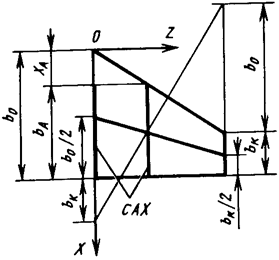
\includegraphics[width=0.7\textwidth]{img/SACH-geometric-construction}
			\captionof{figure}{Геометрическое построение САХ.}
			\label{fig:SACH-geometric-construction}
		\end{minipage}
		\hfill
		\begin{minipage}{0.49\textwidth}
			\centering
			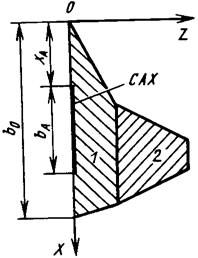
\includegraphics[width=0.5\textwidth]{img/SACH-complex-wing-shape}
			\captionof{figure}{САХ крыла сложной формы.}
			\label{fig:SACH-complex-wing-shape}
		\end{minipage}
	\end{figure}
	Для трапециевидного крыла (\cref{fig:SACH-geometric-construction}) формулы \eqref{eq:3.3} упрощаются, и мы получаем
	\begin{gather}\label{eq:3.4}
		x_\mathrm{A} = \frac{b_0 + 2b_\mathrm{к}}{b_0 + b_\mathrm{к}}\frac{l}{6}\tg\chi_\mathrm{п.к};\quad
		b_\mathrm{A} = \frac{2}{3}\left(b_0 + b_\mathrm{к} - \frac{b_0 b_\mathrm{к}}{b_0 + b_\mathrm{к}}\right).
	\end{gather}\n
	Координата $x_\mathrm{A}$ носка САХ и величина $b_\mathrm{A}$ крыла с изломом кромок (\cref{fig:SACH-complex-wing-shape}) определяются следующими соотношениями:
	\begin{gather}\label{eq:3.5}
		x_\mathrm{A} = \frac{x_\mathrm{A1}S_1 + x_\mathrm{A2}S_2}{S_1 + S_2};\quad
		b_\mathrm{A} = \frac{b_\mathrm{A1}S_1 + b_\mathrm{A2}S_2}{S_1 + S_2},
	\end{gather}
	где $b_\mathrm{A1}$ --- средняя аэродинамическая хорда крыла, составленного из секции \textit{1} и симметричной ей секции левого полукрыла; $b_\mathrm{A2}$ --- САХ крыла, составленного из секции \textit{2} и симметричной ей секции левого полукрыла; $x_\mathrm{A1}$, $x_\mathrm{A2}$ --- координаты носков $b_\mathrm{A1}$ и $b_\mathrm{A2}$; $S_1$, $S_2$ --- удвоенные площади секций \textit{1} и \textit{2}.\n
	САХ трапециевидных крыльев можно найти геометрически так, как это показано на \cref{fig:SACH-geometric-construction}.
	
	\subsection{Аэродинамические характеристики профиля и сечения крыла}
	\begin{figure}[htbp]
		\centering
		\begin{minipage}{0.49\textwidth}
			\centering
			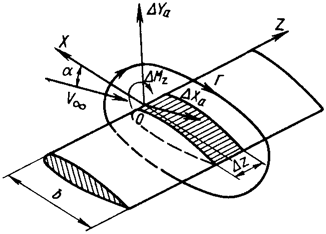
\includegraphics[width=0.75\textwidth]{img/profile-aerodynamic-characteristics-determination}
			\captionof{figure}{Определение аэродинамических характеристик профиля:\\\small{$\Gamma$ --- циркуляция скорости по контуру, охватывающему крыло.}}
			\label{fig:profile-aerodynamic-characteristics-determination}
		\end{minipage}
		\hfill
		\begin{minipage}{0.49\textwidth}
			\centering
			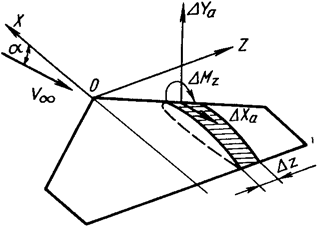
\includegraphics[width=0.75\textwidth]{img/wing-aerodynamic-cross-section-determination}
			\captionof{figure}{Определение аэродинамических характеристик сечения крыла.}
			\label{fig:wing-aerodynamic-cross-section-determination}
		\end{minipage}
	\end{figure}
	Аэродинамическими характеристиками профиля называют аэродинамические характеристики элемента цилиндрического крыла (имеющего форму цилиндра) бесконечного размаха, на которое поток набегает перпендикулярно передней кромке (\cref{fig:profile-aerodynamic-characteristics-determination}):
	\begin{gather}\label{eq:3.6}
		\begin{gathered}
			c_{ya\,\mathrm{пр}} = \frac{\Delta Y_a}{q_\infty b\Delta z} = \lim_{\Delta z \to 0}\frac{\Delta Y_a}{q_\infty b\Delta z};\quad
			c_{xa\,\mathrm{пр}} = \frac{\Delta X_a}{q_\infty b\Delta z} = \lim_{\Delta z \to 0}\frac{\Delta X_a}{q_\infty b\Delta z};\\
			m_{z\,\mathrm{пр}} = \frac{\Delta M_z}{q_\infty b^2\Delta z} = \lim_{\Delta z \to 0}\frac{\Delta M_z}{q_\infty b^2\Delta z},
		\end{gathered}
	\end{gather}
	где $\Delta Y_a$, $\Delta M_z$ --- подъемная сила и момент тангажа, действующие на рассматриваемый элемент; $\Delta X_a$ --- лобовое сопротивление этого элемента; $\Delta z$ --- ширина элемента.\n
	Аэродинамическими характеристиками сечения крыла называют предельные значения аэродинамических характеристик элемента крыла конечного размаха при $\Delta z \to 0$ (\cref{fig:wing-aerodynamic-cross-section-determination}):
	\begin{gather}\label{eq:3.7}
		\begin{gathered}
			c_{ya\,\mathrm{сеч}} = \lim_{\Delta z \to 0}\frac{\Delta Y_a}{q_\infty b_\mathrm{сеч}\Delta z} \cong \frac{\Delta Y_a}{q_\infty b_\mathrm{сеч}\Delta z};\\
			c_{xa\,\mathrm{сеч}} = \lim_{\Delta z \to 0}\frac{\Delta X_a}{q_\infty b_\mathrm{сеч}\Delta z} \cong \frac{\Delta X_a}{q_\infty b_\mathrm{сеч}\Delta z};\\
			m_{z\,\mathrm{сеч}} = \lim_{\Delta z \to 0}\frac{\Delta M_z}{q_\infty b_\mathrm{сеч}^2\Delta z} \cong \frac{\Delta M_z}{q_\infty b_\mathrm{сеч}^2\Delta z},
		\end{gathered}
	\end{gather}
	где $\Delta Y_a$, $\Delta X_a$, $\Delta M_z$ --- силы и момент, действующие на элемент крыла конечного размаха; $b_\mathrm{сеч}$ --- длина хорды сечения.\n
	Так как течение вокруг крыла конечного размаха --- пространственное (трехмерное), а крыло бесконечного размаха обтекается плоскопараллельным (двухмерным) потоком, аэродинамические характеристики профиля и сечения крыла с тем же профилем отличаются друг от друга.\n
	При расчете крыла на прочность, определении его деформаций надо знать погонную нагрузку (силу, действующую на элемент крыла шириной, равной единице). Очевидно, она определяется уравнениями
	\begin{gather}\label{eq:3.8}
		Y_{a\,\mathrm{сеч}} = \lim_{\Delta z \to 0}\frac{\Delta Y_a}{\Delta z} = c_{ya\,\mathrm{сеч}}b_\mathrm{сеч}q_\infty;\quad
		X_{a\,\mathrm{сеч}} = \lim_{\Delta z \to 0}\frac{\Delta X_a}{\Delta z} = c_{xa\,\mathrm{сеч}}b_\mathrm{сеч}q_\infty.
	\end{gather}
	Погонные нагрузки $Y_{a\,\mathrm{сеч}}$, $X_{a\,\mathrm{сеч}}$ называют подъемной силой и лобовым сопротивлением сечения.\n
	Если крыло не закручено и профиль симметричный, то
	\begin{gather}\label{eq:3.9}
		Y_{a\,\mathrm{сеч}} = c_{ya\,\mathrm{сеч}}^\alpha\alpha b_\mathrm{сеч} q_\infty.
	\end{gather}
	Как видно, изменение подъемной силы сечений такого крыла по размаху определяется произведением $c_{ya\,\mathrm{сеч}}^\alpha b_\mathrm{сеч}$. Обычно, рассматривая изменение подъемной силы сечений по размаху, пользуются безразмерной величиной
	\begin{gather}\label{eq:3.10}
		\bar{\Gamma}_\mathrm{пл} = \frac{c_{ya\,\mathrm{сеч}}^\alpha b_\mathrm{сеч}}{c_{ya}^\alpha b_\mathrm{ср}},
	\end{gather}
	представляющей собой относительную погонную нагрузку.
	
	\subsection{Плоские потенциальные течения несжимаемой жидкости}
	
	\subsubsection{Функция тока}
	При исследовании плоских потенциальных потоков кроме потенциала скорости $\varphi$ [см. \eqref{eq:224}] большое значение имеет функция тока. Рассмотрим ее применительно к плоскому установившемуся потенциальному потоку несжимаемой жидкости.\n
	Из уравнения неразрывности \eqref{eq:39} $\frac{\pp v_x}{\pp x} = \frac{\pp\left(-v_y\right)}{\pp y}$. Это равенство означает, что дифференциальный трехчлен $\left(v_x\dd y - v_y\dd x\right)$ равен полному дифференциалу некоторой функции $\psi$:
	\begin{gather}
		v_x\dd y - v_y\dd x = \dd\psi.\label{eq:71}
	\end{gather}\n
	Кроме того, используя уравнение линии тока \eqref{eq:28} $\frac{\dd x}{v_x} = \frac{\dd y}{v_y}$, имеем:
	\begin{gather}
		v_x\dd y - v_y\dd x = 0.\label{eq:72}
	\end{gather}\n
	Сравнивая выражения \eqref{eq:71} и \eqref{eq:72}, получаем, что вдоль линии тока $\dd\psi = 0$, откуда, интегрируя, найдем уравнение семейства линий тока
	\begin{gather}
		\psi\left(x,\; y\right) = C,\label{eq:73}
	\end{gather}
	где $C$ --- произвольная постоянная.\n
	Различным линиям тока соответствуют различные значения постоянной $C$. Функция $\psi$ называется \textit{функцией тока}.\n
	Из соотношения \eqref{eq:71} следует, что составляющие скорости $v_x$ и $v_y$ можно выразить через функцию тока:
	\begin{gather}
		v_x = \frac{\pp\psi}{\pp y}, \quad v_y = -\frac{\pp\psi}{\pp x}.\label{eq:74}
	\end{gather}\n
	Составляющие скорости $v_x$ и $v_y$, представим также в виде производных потенциала скорости $\varphi$ [см. \eqref{eq:224}]:
	\begin{gather}
		v_x = \frac{\pp\varphi}{\pp x}, \quad v_y = \frac{\pp\varphi}{\pp y}.\label{eq:75}
	\end{gather}\n
	Сравнение формул \eqref{eq:74} и \eqref{eq:75} приводит к важному соотношению
	\begin{gather}
		\frac{\pp\varphi}{\pp x} = \frac{\pp\psi}{\pp y}, \quad \frac{\pp\varphi}{\pp y} = -\frac{\pp\psi}{\pp x}.\label{eq:76}
	\end{gather}\n
	Если потенциал скорости $\varphi$, являющийся функцией координат $x$ и $y$, приравнять постоянной $\varphi\left(x,\; y\right) = C$, то, очевидно, будем иметь семейство линий, обладающих тем свойством, что вдоль каждой такой линии потенциал скорости сохраняет постоянное значение. Такие линии называются \textit{эквипотенциальными}.\n
	Из формул \eqref{eq:76} следует соотношение между функциями $\varphi$ и $\psi$, т. е. $\frac{\pp\varphi}{\pp x}\frac{\pp\psi}{\pp x} + \frac{\pp\varphi}{\pp y}\frac{\pp\psi}{\pp y} = 0$. Это соотношение является условием ортогональности кривых $\varphi\left(x,\; y\right) = C$ и $\psi\left(x,\; y\right) = C$. Таким образом, в плоском установившемся потенциальном потоке семейство линий тока и семейство эквипотенциальных линий ортогональны.\n
	Потенциал скорости и функция тока удовлетворяют уравнению Лапласа:
	\begin{gather}
		\frac{\pp^2\varphi}{\pp x^2} + \frac{\pp^2\varphi}{\pp y^2} = 0;\label{eq:77}\\
		\frac{\pp^2\psi}{\pp x^2} + \frac{\pp^2\psi}{\pp y^2} = 0.\label{eq:78}
	\end{gather}\n
	Уравнение \eqref{eq:77} следует из уравнения неразрывности $\frac{\pp v_x}{\pp x} + \frac{\pp v_y}{\pp y} = 0$ после подстановки в него выражений \eqref{eq:75}, а уравнение \eqref{eq:78} --- из условия потенциальности потока $\frac{\pp v_y}{\pp x} - \frac{\pp v_x}{\pp y} = 0$ в результате использования выражений \eqref{eq:74}.
	
	\subsubsection{Метод наложения потенциальных потоков}
	В исследовании потенциальных потоков большое практическое значение имеет метод наложения потенциальных потоков, заключающийся в следующем. Пусть имеется два потенциальных потока, обладающих потенциалами $\varphi_1$ и $\varphi_2$, удовлетворяющими уравнению Лапласа \eqref{eq:77}:
	\begin{gather*}
		\frac{\pp^2\varphi_1}{\pp x^2} + \frac{\pp^2\varphi_1}{\pp y^2} = 0; \quad \frac{\pp^2\varphi_2}{\pp x^2} + \frac{\pp^2\varphi_2}{\pp y^2} = 0.
	\end{gather*}\n
	В таком случае вследствие линейности этого уравнения потенциал скорости, равный их сумме $\varphi = \varphi_1 + \varphi_2$, также удовлетворяет уравнению Лапласа, т. е. представляет собой некоторый новый поток несжимаемой жидкости.\n
	Новый сложный поток с потенциалом $\varphi = \varphi_1 + \varphi_2$, является результатом наложения двух исходных потоков, т. е. результатом геометрического суммирования в каждой точке пространства скоростей первого и второго потоков, так как для сложного потока $v_x = \frac{\pp\varphi}{\pp x} = \frac{\pp\varphi_1}{\pp x} + \frac{\pp\varphi_2}{\pp x} = v_{1_x} + v_{2_x}; \quad v_y = \frac{\pp\varphi}{\pp y} = \frac{\pp\varphi_1}{\pp y} + \frac{\pp\varphi_2}{\pp y} = v_{1_y} + v_{2_y}$.\n
	Аналогично можно показать, что для нового сложного потока функция тока $\psi = \psi_1 + \psi_2$.\n
	Следовательно, наложение двух (и более) потоков сводится к простому алгебраическому суммированию потенциалов и функций тока исходных потоков. Поэтому, имея ряд решений, соответствующих некоторым простейшим течениям жидкости, путем суммирования их в различных сочетаниях можно получить решения, соответствующие более сложным течениям.
	
	\subsubsection{Комплексный потенциал}
	Эффективным методом изучения свойств плоского течения является метод комплексного переменного, получивший в аэродинамике большое применение. Основные функции, характеризующие свойства плоского потенциального течения, --- функция тока $\psi\left(x,\; y\right)$ и потенциал скорости $\varphi\left(x,\; y\right)$ определяются соотношениями \eqref{eq:76}.\n
	В теории функции комплексного переменного эти соотношения, как известно, носят названия \textit{уравнений Коши-Римана} и выражают то условие, что комплексная комбинация из этих функций от двух действительных переменных, т. е. $\varphi\left(x,\; y\right) + i\psi\left(x,\; y\right)$, является аналитической функцией комплексного переменного $z = x + iy$. Обозначим эту функцию
	\begin{gather}
		w\left(z\right) = \varphi + i\psi.\label{eq:79}
	\end{gather}\n
	Функцию $w\left(z\right)$ называют \textit{комплексным потенциалом или характеристической функцией течения}.\n
	Как показано ниже, комплексный потенциал $w\left(z\right)$ дает возможность использовать хорошо разработанный аппарат теории функций комплексного переменного для решения задачи об обтекании тел и играет исключительно важную роль в аэродинамике плоскопараллельных течений.\n
	Введем понятие о комплексной скорости. Возьмем производную от комплексного потенциала $w\left(z\right)$ по комплексному переменному $z$. Как известно из теории функций комплексного переменного, производная $\frac{\dd w}{\dd z} = \frac{\pp\varphi}{\pp x} + i\frac{\pp\psi}{\pp x} = -i\frac{\pp\varphi}{\pp y} + \frac{\pp\psi}{\pp y}$. Отсюда, используя выражения \eqref{eq:74}, получаем
	\begin{gather}
		\frac{\dd w}{\dd z} = v_x - iv_y.\label{eq:710}
	\end{gather}\n
	\begin{figure}[htbp]
		\centering
		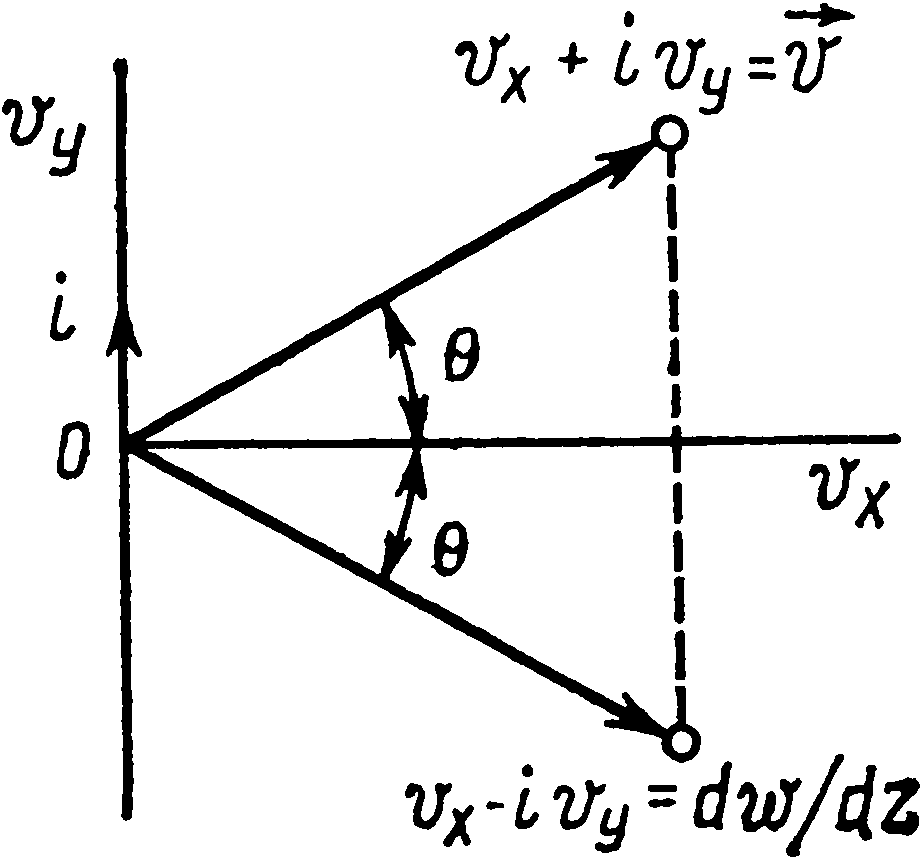
\includegraphics[width=0.25\linewidth]{img/complex-velocity-definition}
		\caption{Определение комплексной скорости.}
		\label{fig:7.1_complex-velocity-definition}
	\end{figure}
	Производная $\frac{\dd w}{\dd z}$ называется \textit{комплексной скоростью}. Очевидно, модуль комплексной скорости будет давать значение самой скорости $v$. Комплексную скорость можно интерпретировать геометрически как вектор, представляющий собой зеркальное отображение относительно действительной оси вектора скорости $v_x + iv_y$ (\cref{fig:7.1_complex-velocity-definition}). Выражению \eqref{eq:710} для комплексной скорости можно придать также и другой вид. Для этого представим составляющие скорости $v_x$, $v_y$ в виде $v_x = v\cos\varTheta^*$, $v_y = v\sin\varTheta^*$ ($\varTheta^*$ --- угол наклона $\vv{v}$). Тогда
	\begin{gather}
		\frac{\dd w}{\dd z} = v\left(\cos\varTheta^* - i\sin\varTheta^*\right) = v\mathrm{e}^{-i\varTheta^*}.\label{eq:711}
	\end{gather}\n
	Из выражений \eqref{eq:79} -- \eqref{eq:711} следует, что если известен комплексный потенциал потока, то достаточно просто можно определить линии тока $\psi = C$, где функция тока $\psi$ равна мнимой части комплексного потенциала: $\psi = \mathrm{Jm}\left[w\left(z\right)\right]$, а также направление и значение скорости потока в любой точке (по значению производной комплексного потенциала $\frac{\dd w}{\dd z}$).
	
	\subsubsection{Примеры плоскопараллельных потенциальных течений}
	Рассмотрим прежде всего наиболее характерные примеры простейших плоских установившихся потенциальных потоков, комбинацией (наложением) которых можно получить сложные практически важные потоки.
	\paragraph{Прямолинейный равномерный поток.} Предположим, что плоское течение задано комплексным потенциалом
	\begin{subequations}
		\begin{gather}
			w = az,\label{eq:712}
		\end{gather}
		где $a = a_1 - ia_2$ --- комплексная величина.\n
		Требуется определить характер течения.\n
		Подставляя в \eqref{eq:712} выражения $w$, $a$ и $z$, получаем $\varphi + i\psi = \left(a_1 - ia_2\right)\left(x + iy\right)$, откуда, приравнивая действительные и мнимые части, находим $\varphi = a_1 x + a_2 y$, $\psi = -a_2 x + a_1 y$.\n
		Приравнивая функции $\varphi$ и $\psi$ постоянным, составляем уравнения эквипотенциальных линий и линий тока:
		\begin{gather*}
			a_1 x + a_2 y = C_1, \quad -a_2 x + a_1 y = C_2,
		\end{gather*}
		т. е. уравнения семейств взаимно ортогональных прямых. В этом случае комплексная скорость $\frac{\dd w}{\dd z} = a = a_1 - ia_2$. Следовательно, поток течет по прямым, наклоненным к оси $x$ под углом $\alpha\left(\tg\alpha = a_2/a_1\right)$, со скоростью $v = \left|\frac{\dd w}{\dd z}\right| = \sqrt{a_1^2 + a_2^2}$.\n
		При $a_2 = 0 \left(a = a_1 > 0\right)$ получим поток вдоль оси $x$ со скоростью $v = a$. Комплексный потенциал такого потока имеет вид
		\begin{gather}
			w\left(z\right) = vz.\label{eq:712'}
		\end{gather}
	\end{subequations}
	\begin{figure}[htbp]
		\centering
		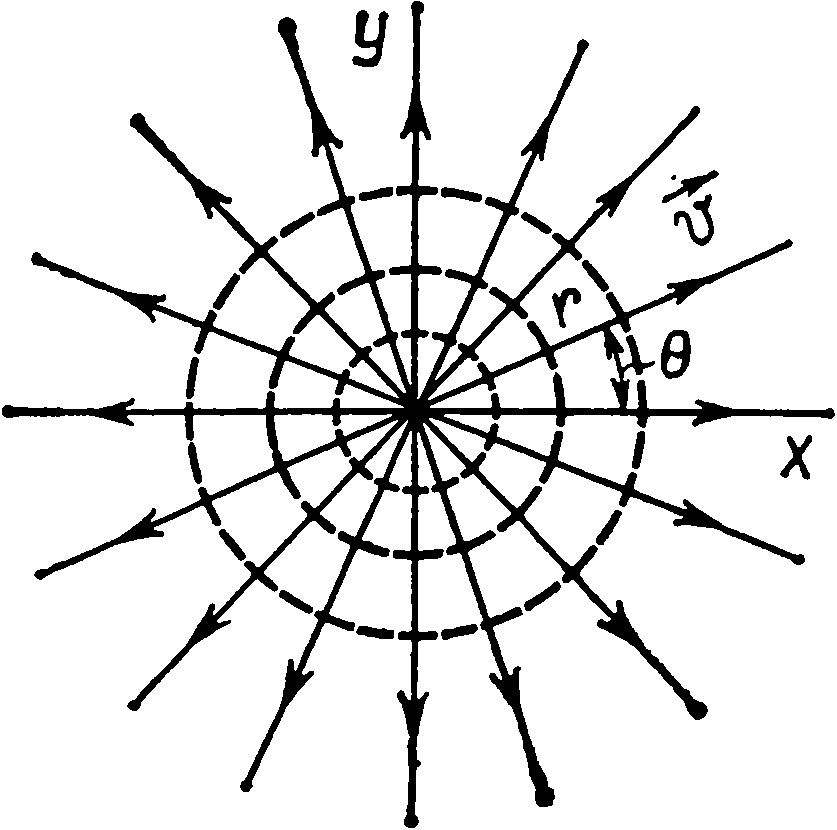
\includegraphics[width=0.25\linewidth]{img/source-at-the-origin}
		\caption{Источник в начале координат.}
		\label{fig:7.2_source-at-the-origin}
	\end{figure}
	\paragraph{Источник и сток.} Пусть поток задан комплексным потенциалом
	\begin{gather}
		w\left(z\right) = \ln z.\label{eq:713}
	\end{gather}\n
	В этом случае для исследования характера течения жидкости удобнее пользоваться представлением комплексной координаты $z$ через полярные координаты рассматриваемой точки $r$ и $\varTheta$ (\cref{fig:7.2_source-at-the-origin}): $z = r\mathrm{e}^{i\varTheta}$. Тогда $w\left(z\right) = \varphi + i\psi = \ln r + i\varTheta$, откуда $\varphi = \ln r$, $\psi = \varTheta$.\n
	Очевидно, линии тока $\psi = \varTheta = C$ представляют собой семейство лучей, исходящих из начала координат, т. е. начало координат является источником. Покажем, что направление течения соответствует направлению, показанному на \cref{fig:7.2_source-at-the-origin}. Для этого найдем комплексную скорость: $\frac{\dd w}{\dd z} = \frac{1}{z} = \frac{1}{r}\mathrm{e}^{-i\varTheta}$. Отсюда, используя выражение \eqref{eq:711}, найдем значение скорости потока
	\begin{gather}
		v = \frac{1}{r}\label{eq:714}
	\end{gather}
	и угол наклона вектора скорости $\varTheta^* = \varTheta$, т. е. направление потока совпадает с положительным направлением полярного радиуса. Следовательно, комплексный потенциал \eqref{eq:713} соответствует потоку от источника, расположенного в начале координат.\n
	Заметим, что в рассматриваемом примере начало координат является особой точкой: для функции $w$ --- изолированной логарифмической точкой, а для комплексной скорости $\frac{\dd w}{\dd z}$ --- полюсом первого порядка, так как при $z = 0 \left(r = 0\right)$ величины $w$ и $\frac{\dd w}{\dd z}$ бесконечны. Формулой \eqref{eq:714} можно пользоваться во всех точках, за исключением начала координат.\n
	Найдем удельный расход жидкости $Q$, т. е. количество жидкости, вытекающей в единицу времени из источника. Удельный расход принято называть \textit{мощностью источника}. Она равна $Q = v2\pi r$. Подставляя сюда выражение \eqref{eq:714} для рассматриваемого примера, имеем $Q = 2\pi$.\n
	Следовательно, в общем случае комплексный потенциал источника мощностью $Q$
	\begin{gather}
		w\left(z\right) = \frac{Q}{2\pi}\ln z.\label{eq:715}
	\end{gather}\n
	Если источник находится не в начале координат, а в точке $z = a$, то
	\begin{gather}
		w\left(z\right) = \frac{Q}{2\pi}\ln\left(z - a\right).\label{eq:716}
	\end{gather}\n
	Случай, когда жидкость течет в обратном направлении, т. е. втекает в начало координат по прямолинейным лучам, соответствует стоку. Очевидно, что функция $w\left(z\right)$ для стока мощностью $Q$ отличается от аналогичной функции для источника только знаком, т. е.
	\begin{gather}
		w\left(z\right) = -\frac{Q}{2\pi}\ln z \quad \mathrm{и} \quad w\left(z\right) = -\frac{Q}{2\pi}\ln\left(z - a\right).\label{eq:717}
	\end{gather}
	\begin{figure}[htbp]
		\centering
		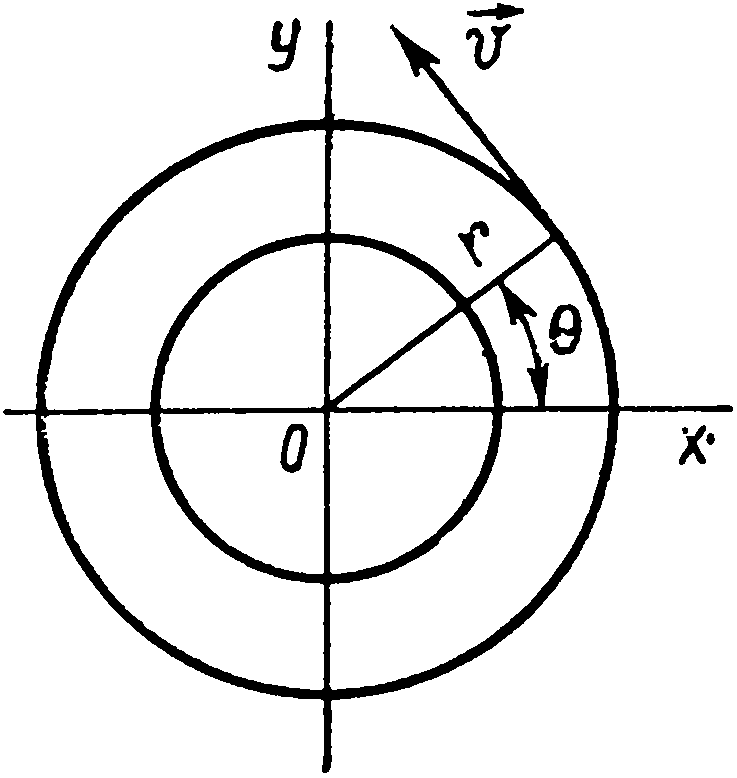
\includegraphics[width=0.25\linewidth]{img/vortex-at-the-origin}
		\caption{Вихрь в начале координат.}
		\label{fig:7.3_vortex-at-the-origin}
	\end{figure}
	\paragraph{Вихрь.} Зададим комплексный потенциал в виде
	\begin{gather}
		w\left(z\right) = -\frac{i\Gamma}{2\pi}\ln z,\label{eq:718}
	\end{gather}
	т. е. линии тока представляют собой семейство концентрических окружностей $r = C$ (\cref{fig:7.3_vortex-at-the-origin}).\n
	Для установления направления потока найдем комплексную скорость: $\frac{\dd w}{\dd z} = -\frac{i\Gamma}{2\pi}\frac{1}{z}$, или $\frac{\dd w}{\dd z} = \frac{\Gamma}{2\pi r}\mathrm{e}^{-i\left(\pi/2 + \varTheta\right)}$. Отсюда, используя выражение \eqref{eq:711}, найдем
	\begin{gather}
		v = \frac{\Gamma}{2\pi r},\label{eq:719}
	\end{gather}
	а $\varTheta^* = \pi/2 + \varTheta$, т. е. движение жидкости совершается в сторону возрастания угла $\varTheta$, т. е. против часовой стрелки.\n
	Таким образом, все частицы жидкости движутся по концентрическим окружностям с постоянной для данной окружности скоростью. Это означает, что вдоль оси, перпендикулярной плоскости $x$, $y$ и проходящей через начало координат, расположен бесконечно длинный прямолинейный вихрь, вызывающий в перпендикулярной ему плоскости движение частиц жидкости по концентрическим окружностям.\n
	Постоянная $\Gamma$ в выражении \eqref{eq:718} представляет собой циркуляцию скорости по любому замкнутому контуру, охватывающему начало координат. Действительно, циркуляция скорости по окружности с центром в точке $O$ при этом равна $v2\pi r$. Подставляя сюда выражение \eqref{eq:719}, получаем, что она равна постоянной $\Gamma$. Как и в случае источника, начало координат является особой точкой.\n
	Если вихрь находится не в начале координат, а в точке $z = a$, то $w = -\frac{i\Gamma}{2\pi}\ln\left(z - a\right)$. В общем случае
	\begin{gather}
		w = \pm\frac{i\Gamma}{2\pi}\ln\left(z - a\right),\label{eq:720}
	\end{gather}
	где знак <<$+$>> соответствует направлению вращения вихря по часовой стрелке, а знак <<$-$>> --- против часовой стрелки.
	\begin{figure}[htbp]
		\centering
		\begin{minipage}{0.49\textwidth}
			\centering
			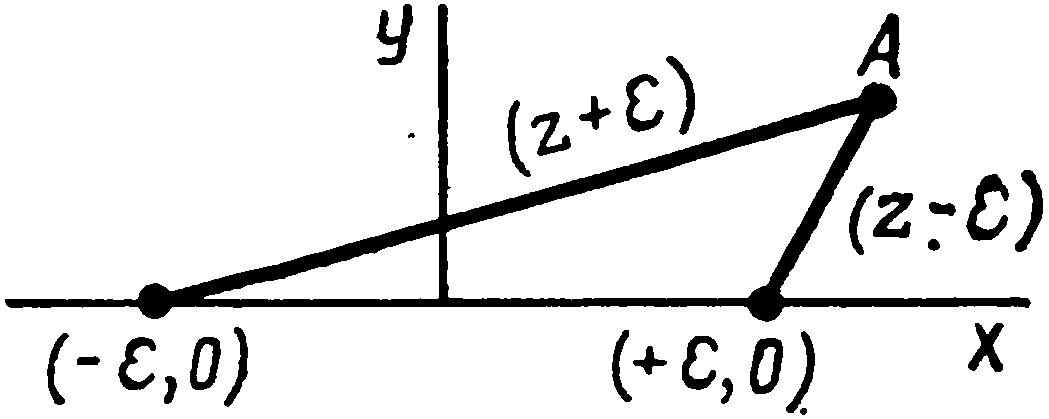
\includegraphics[width=0.7\textwidth]{img/dipole-complex-potential-scheme}
			\captionof{figure}{Схема для определения комплексного потенциала диполя.}
			\label{fig:7.4_dipole-complex-potential-scheme}
		\end{minipage}
		\hfill
		\begin{minipage}{0.49\textwidth}
			\centering
			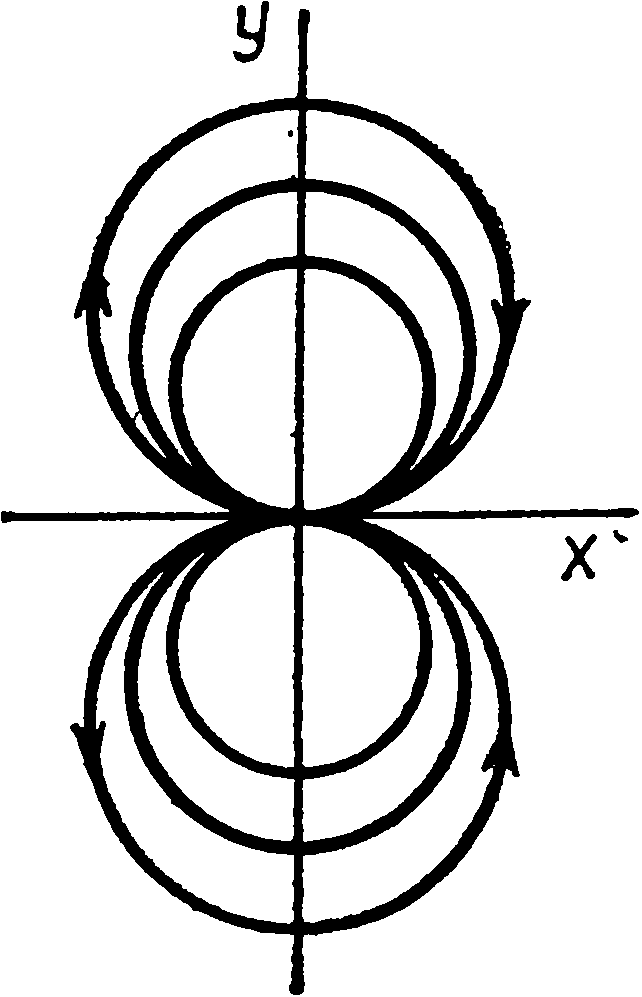
\includegraphics[width=0.35\textwidth]{img/dipole-at-the-origin}
			\captionof{figure}{Диполь в начале координат с осью вдоль оси $x$.}
			\label{fig:7.5_dipole-at-the-origin}
		\end{minipage}
	\end{figure}
	\paragraph{Диполь на плоскости.} \textit{Диполем} называется комбинация источника и стока одинаковой мощности, помещенных на бесконечно малом расстоянии друг от друга. Сближая источник и сток, предполагаем, что мощности их неограниченно возрастают так, что в пределе произведение $Q2\varepsilon$ стремится к некоторой конечной величине $m$, называемой \textit{моментом диполя}. Прямая, соединяющая источник и сток, называется \textit{осью диполя}.\n
	Рассмотрим диполь с осью вдоль оси $x$ (\cref{fig:7.4_dipole-complex-potential-scheme}). Предположим, что в точке $\left(-\varepsilon,\; 0\right)$ расположен источник, а в точке $\left(+\varepsilon,\; 0\right)$ --- сток. Используя метод наложения потенциальных потоков, найдем суммарный комплексный потенциал:
	\begin{gather*}
		w = w_1 + w_2 = \frac{Q}{2\pi}\ln\frac{z + \varepsilon}{z - \varepsilon}.
	\end{gather*}\n
	Переходя к пределу при $\varepsilon\rightarrow 0$, получаем комплексный потенциал диполя в начале координат с моментом $m$ и осью вдоль оси $x$ в виде
	\begin{gather}
		w\left(z\right) = \frac{m}{2\pi}\frac{1}{z}.\label{eq:721}
	\end{gather}\n
	Отсюда найдем функцию тока $\psi = -\frac{m}{2\pi}\frac{y}{x^2 + y^2}$ и уравнение семейства линий тока $\frac{y}{x^2 + y^2} = C$, откуда $x^2 + \left(y - \frac{1}{2C}\right)^2 = \frac{1}{4C^2}$.\n
	Очевидно, совокупность линий тока представляет собой семейство окружностей с центрами на оси $y$, касающихся оси $x$ в начале координат (\cref{fig:7.5_dipole-at-the-origin}). Таким образом, жидкость по указанным окружностям вытекает из начала координат и вновь в него втекает. Очевидно, в этом случае расход жидкости через произвольный замкнутый контур, окружающий диполь, равен нулю. Если же диполь расположен в точке $z = a$, то комплексный потенциал имеет вид
	\begin{gather}
		w\left(z\right) = \frac{m}{2\pi}\frac{1}{z - a}.\label{eq:722}
	\end{gather}
	
	\subsection{Обтекание цилиндра}\label{sec:7.2}
	Рассмотрим обтекание цилиндра круглого сечения при $\Gamma = 0$ (бесциркуляционное обтекание) и $\Gamma\ne 0$ (циркуляционное обтекание).
	
	\subsubsection{Бесциркуляционное обтекание цилиндра}
	\begin{figure}[htbp]
		\centering
		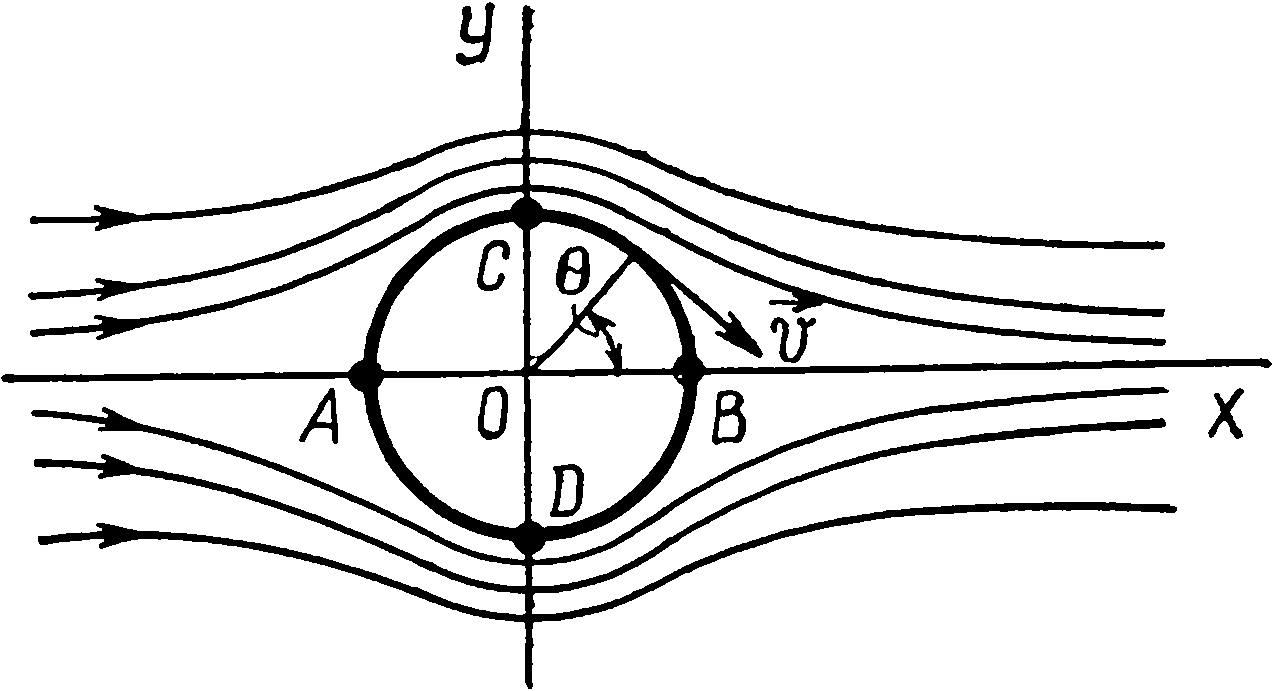
\includegraphics[width=0.35\linewidth]{img/non-circulating-flow-around-a-cylinder}
		\caption{Бесциркуляционное обтекание круглого цилиндра.}
		\label{fig:7.6_non-circulating-flow-around-a-cylinder}
	\end{figure}
	Наложим друг на друга два потока: равномерный прямолинейный поток, движущийся в направлении оси $x$ со скоростью $v_\infty$, и поток, получаемый от диполя, расположенного в начале координат, с осью вдоль оси $x$ и моментом $m$.\n
	Для нахождения комплексного потенциала сложного течения нужно сложить комплексные потенциалы исходных потоков \eqref{eq:712'} и \eqref{eq:721}. Следовательно, в рассматриваемом случае комплексный потенциал имеет вид
	\begin{gather}
		w\left(z\right) = v_\infty\left(z + \frac{m}{2\pi v_\infty}\frac{1}{z}\right).\label{eq:723}
	\end{gather}\n
	Отсюда найдем функцию тока:
	\begin{gather*}
		\psi = v_\infty\left(y - \frac{m}{2\pi v_\infty}\frac{y}{x^2 + y^2}\right).
	\end{gather*}\n
	Чтобы найти линии тока, приравняем функцию тока постоянной $y - \frac{m}{2\pi v_\infty}\frac{y}{x^2 + y^2} = C$, откуда $y\left[\left(x^2 + y^2\right) - \frac{m}{2\pi v_\infty}\right] = C\left(x^2 + y^2\right)$.\n
	Как видим, линии тока представляют собой семейство кривых третьего порядка. Для выяснения характера течений найдем нулевую линию тока, соответствующую $C = 0$. Для нулевой линии тока получаем два уравнения: $y = 0$ и $x^2 + y^2 = \frac{m}{2\pi v_\infty}$.\n
	Следовательно, нулевая линия тока представляет собой участок оси $x$ и окружность радиусом $r = \sqrt{\frac{m}{2\pi v_\infty}}$ с центром в начале координат. Принимая указанную окружность за твердую границу и рассматривая течение жидкости вне этой окружности, можно трактовать полученный поток как поток, обтекающий бесконечно длинный цилиндр радиусом $r = \sqrt{\frac{m}{2\pi v_\infty}}$.\n
	Для того чтобы получить обтекание цилиндра заданного радиусом $r_0$, необходимо подобрать момент диполя из условия $r_0^2 = \frac{m}{2\pi v_\infty}$, т. е.
	\begin{gather}
		m = 2\pi v_\infty r_0^2.\label{eq:724}
	\end{gather}\n
	Таким образом, в рассматриваемом случае воздействие цилиндра на поток заменяется воздействием диполя. Задавая постоянной $C$ различные значения, получаем семейство линий тока в окрестности цилиндра (\cref{fig:7.6_non-circulating-flow-around-a-cylinder}).\n
	Подставляя выражение \eqref{eq:724} в формулу \eqref{eq:723}, получаем комплексный потенциал потока, обтекающего цилиндр радиусом $r_0$:
	\begin{gather}
		w = v_\infty\left(z + \frac{r_0^2}{z}\right).\label{eq:725}
	\end{gather}\n
	Найдем распределение скорости по поверхности цилиндра. Для этого, как и в предыдущих примерах, достаточно определить производную $\frac{\dd w}{\dd z} = v_\infty\left(1 - \frac{r_0^2}{z^2}\right)$.\n
	На поверхности цилиндра (\cref{fig:7.6_non-circulating-flow-around-a-cylinder}) $z = r_0\mathrm{e}^{i\varTheta}$. Тогда
	\begin{gather*}
		\frac{\dd w}{\dd z} = v_\infty\left(1 - \mathrm{e}^{-2i\varTheta}\right) = i\mathrm{e}^{-i\varTheta}2v_\infty\sin\varTheta.
	\end{gather*}\n
	Отсюда найдем скорость потока:
	\begin{gather}
		v = 2v_\infty\left|\sin\varTheta\right|.\label{eq:726}
	\end{gather}\n
	Из формулы \eqref{eq:726} следует, что распределение скорости по верхней и нижней поверхностям цилиндра симметрично. При этом циркуляция скорости $\Gamma = 0$. В точках $A\left(\varTheta = \pi\right)$ и $B\left(\varTheta = 0\right)$ скорости потока равны нулю $\left(v = 0\right)$. Эти точки называются \textit{критическими}. В точках $C\left(\varTheta = \pi/2\right)$ и $D\left(\varTheta = -\pi/2\right)$ скорость принимает максимальное значение, не зависящее от радиуса цилиндра и равное удвоенной скорости на бесконечности: $v = 2v_\infty$.\n
	Вычислим давление на цилиндре, используя уравнение Бернулли: $p = p_\infty + \frac{\rho v_\infty^2}{2} - \frac{\rho v^2}{2}$. Подставляя скорости $v$ из \eqref{eq:726}, находим
	\begin{gather*}
		p - p_\infty = \left(1 - 4\sin^2\varTheta\right)\frac{\rho v_\infty^2}{2}.
	\end{gather*}\n
	Введя безразмерный коэффициент давления $\bar{p} = \frac{\left(p - p_\infty\right)}{\rho v_\infty^2/2}$, имеем
	\begin{gather}
		\bar{p} = 1 - 4\sin^2\varTheta.\label{eq:727}
	\end{gather}\n
	Как видим, безразмерный коэффициент давления не зависит от $v_\infty$ и $p_\infty$. При $\varTheta = 0,\; \pi$ (в точках $B$ и $A$) $\bar{p} = 1$, а при $\varTheta = \pi/2, -\pi/2$ (в точках $C$ и $D$) $\bar{p} = \bar{p}_\mathrm{min} = -3$, т. е. в этих точках наблюдается максимальное разрежение.\n
	Из симметричного распределения давления по цилиндру следует, что результирующая сила давления потока на цилиндр равна нулю, т. е. при этом тело не испытывает сопротивления. В этом заключается известный парадокс Эйлера-Даламбера. Этот результат можно распространить и на случай произвольного контура при его безотрывном обтекании потоком идеальной несжимаемой жидкости.\n
	\begin{figure}[htbp]
		\centering
		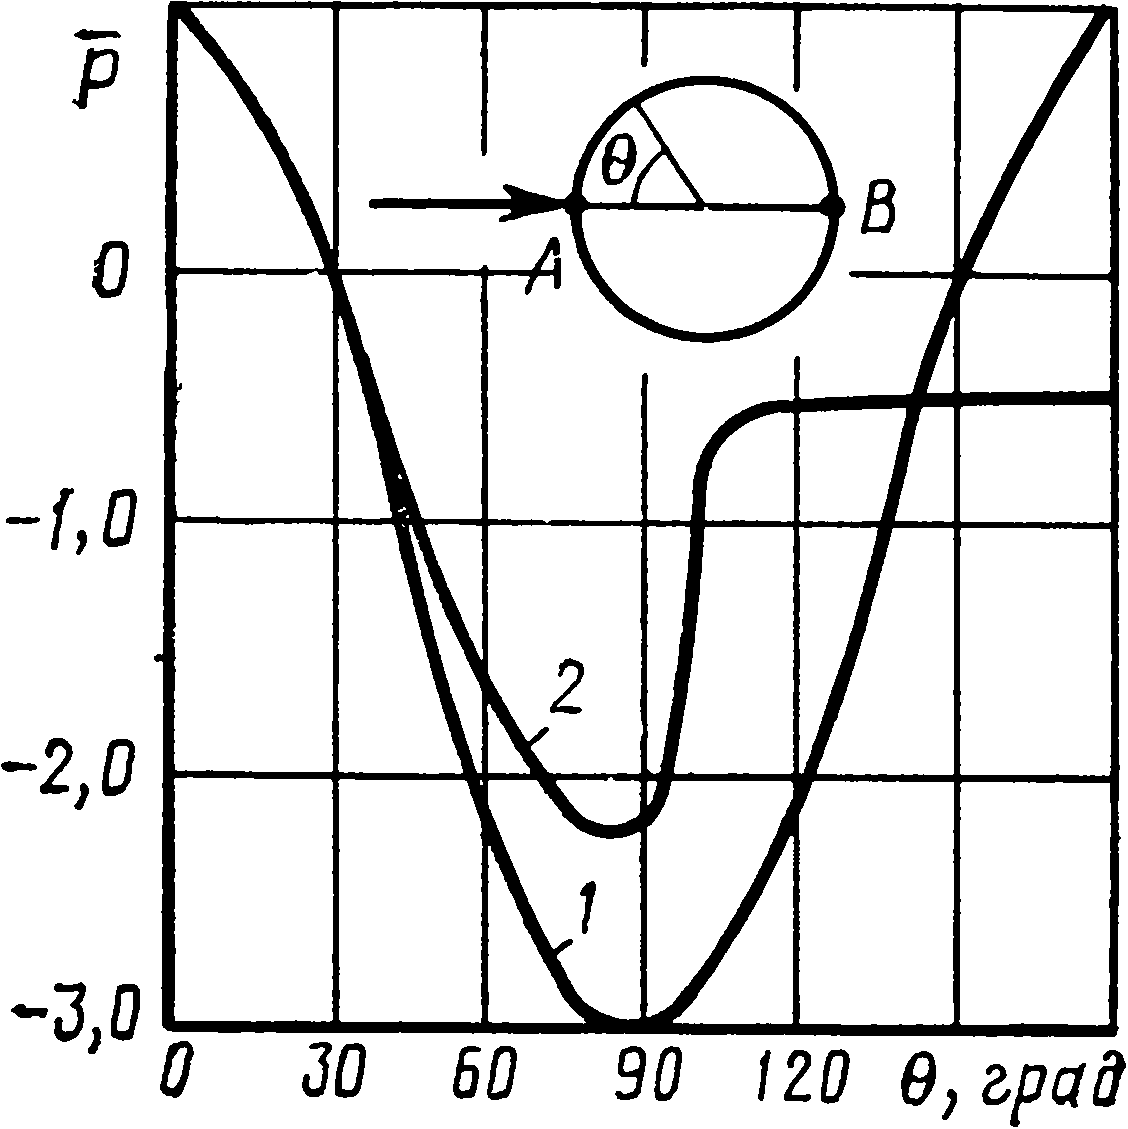
\includegraphics[width=0.3\linewidth]{img/pressure-coefficient-on-cylinder-change}
		\caption{Изменение коэффициента давления в зависимости от положения точки (угла $\varTheta$) на поверхности цилиндра:\\\small{\textit{1} --- теоретические данные; \textit{2} --- экспериментальные данные.}}
		\label{fig:7.7_pressure-coefficient-on-cylinder-change}
	\end{figure}
	На \cref{fig:7.7_pressure-coefficient-on-cylinder-change} приведена теоретическая кривая \textit{1} распределения коэффициента давления $\bar{p}$ по поверхности $\bar{p} = f\left(\varTheta\right)$, рассчитанная по формуле \eqref{eq:727}. Там же для сравнения представлена экспериментальная \textit{2} кривая $\bar{p} = F\left(\varTheta\right)$. Из \cref{fig:7.7_pressure-coefficient-on-cylinder-change} видно, что теоретическая кривая существенно отличается от экспериментальной в кормовой части цилиндра. Это объясняется тем, что на этом участке поверхности реальный поток вязкой жидкости (газа) перестает омывать цилиндр и отрывается от него, образуя за ним вихревую область.
	
	\subsubsection{Циркуляционное обтекание цилиндра}
	Чтобы получить циркуляционное обтекание круглого цилиндра, наложим на рассмотренное выше течение чисто циркуляционный поток от плоского вихря, расположенного в начале координат с направлением вращения по часовой стрелке. Сложив комплексные потенциалы указанных потоков \eqref{eq:725} и \eqref{eq:720}, получим
	\begin{gather}
		w\left(z\right) = v_\infty\left(z + \frac{r_0^2}{z}\right) + \frac{i\Gamma}{2\pi}\ln z.\label{eq:728}
	\end{gather}\n
	В этом случае в каждой точке пространства к скорости бесциркуляционного потока, обтекающего цилиндр, прибавляется скорость от чисто циркуляционного потока. Наложение циркуляционного потока нарушает симметрию линий тока, так как на верхней поверхности скорость от чисто циркуляционного потока направлена в ту же сторону, что и скорость бесциркуляционного потока, а внизу скорость чисто циркуляционного потока направлена в обратную сторону. Вследствие сложения скоростей над цилиндром образуется область повышенных, а под цилиндром --- область пониженных скоростей. Суммарная скорость потока на поверхности цилиндра
	\begin{gather}
		v = \left|2v_\infty\sin\varTheta + \frac{\Gamma}{2\pi r_0}\right|.\label{eq:729}
	\end{gather}\n
	\begin{figure}[htbp]
		\centering
		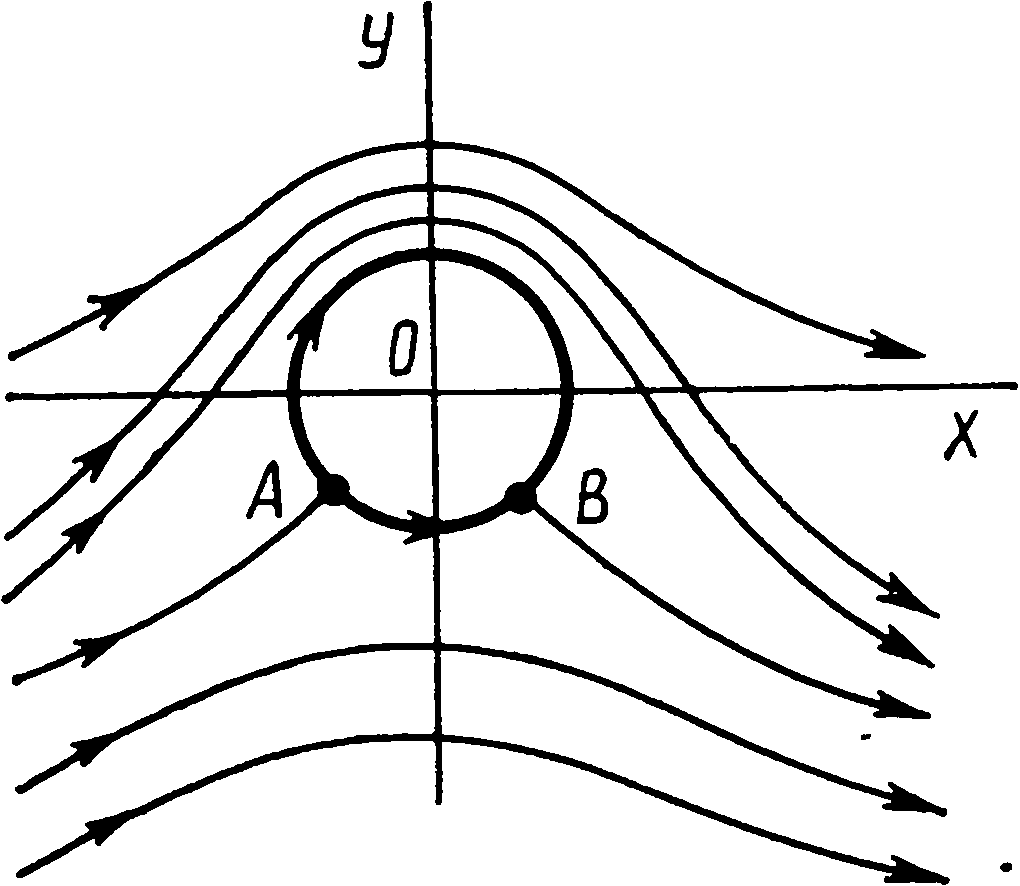
\includegraphics[width=0.3\linewidth]{img/circulating-flow-around-a-cylinder}
		\caption{Циркуляционное обтекание круглого цилиндра в случае $\Gamma < 4\pi v_\infty r_0$.}
		\label{fig:7.8_circulating-flow-around-a-cylinder}
	\end{figure}
	Критические точки $A$ и $B$ (\cref{fig:7.8_circulating-flow-around-a-cylinder}) в этом случае сходят с оси $x$ и располагаются на нижней поверхности цилиндра. Найдем угол $\varTheta_\mathrm{кр}$, определяющий положение критических точек, для чего приравняем нулю скорость потока \eqref{eq:729}. Тогда
	\begin{gather}
		\sin\varTheta_\mathrm{кр} = -\frac{\Gamma}{4\pi v_\infty r_0}.\label{eq:730}
	\end{gather}\n
	Очевидно, значению $\Gamma < 4\pi v_\infty r_0$ соответствуют две критические точки $A$ и $B$. Как видно из формулы \eqref{eq:730}, с увеличением $\Gamma$ критические точки смещаются вниз. В случае, когда $\Gamma = 4\pi v_\infty r_0$, получаем $\sin\varTheta_\mathrm{кр} = -1$, т. е. критические точки сливаются в одну точку. При дальнейшем увеличении $\Gamma$, т. е. при $\Gamma > 4\pi v_\infty r_0$, критическая точка сходит с цилиндра.\n
	На \cref{fig:7.8_circulating-flow-around-a-cylinder} показан характер обтекания цилиндра, соответствующий случаю $\Gamma < 4\pi v_\infty r_0$.\n
	Найдем распределение давления по поверхности цилиндра. Используя уравнение Бернулли $p + \frac{\rho v^2}{2} = p_\infty + \frac{\rho v_\infty^2}{2}$, для определения коэффициента давления $\bar{p} = \frac{p - p_\infty}{\rho v_\infty^2/2}$ получим $p = 1 - v^2/v_\infty^2$. Подставляя сюда выражение \eqref{eq:729}, имеем
	\begin{gather}
		\bar{p} = 1 - \left(2\sin\varTheta + \frac{\Gamma}{2\pi v_\infty r_0}\right)^2.\label{eq:731}
	\end{gather}\n
	Из формулы \eqref{eq:731} следует, что распределение коэффициента давления симметрично относительно оси $y$. Поэтому при циркуляционном обтекании цилиндра, так же как при $\Gamma = 0$, сопротивление равно нулю: $X_\mathrm{a} = 0$ (парадокс Эйлера-Даламбера). При этом подъемная сила не равна нулю. Она определяется по формуле Жуковского.
	
	\subsection{Формула Жуковского}
	В основе современной теории крыла лежит \textit{теорема Жуковского} о результирующей силе давления потока на обтекаемое им тело. Н. Е. Жуковский, используя модель идеальной жидкости, предложил искать источник силового воздействия потока на тело в образовании циркуляции.\n
	Поясним это на частном случае обтекания круглого цилиндра. Как показано выше, при бесциркуляционном обтекании цилиндра скорости и давления распределяются симметрично, что приводит к отсутствию результирующей силы давления. Если цилиндр обтекается с циркуляцией, то симметрия в распределении скоростей и давлений относительно оси $x$ нарушается, в результате чего появляется подъемная сила. Образование циркуляции можно представить как результат воздействия на поток вихря, расположенного вдоль оси цилиндра.\n
	\begin{figure}[htbp]
		\centering
		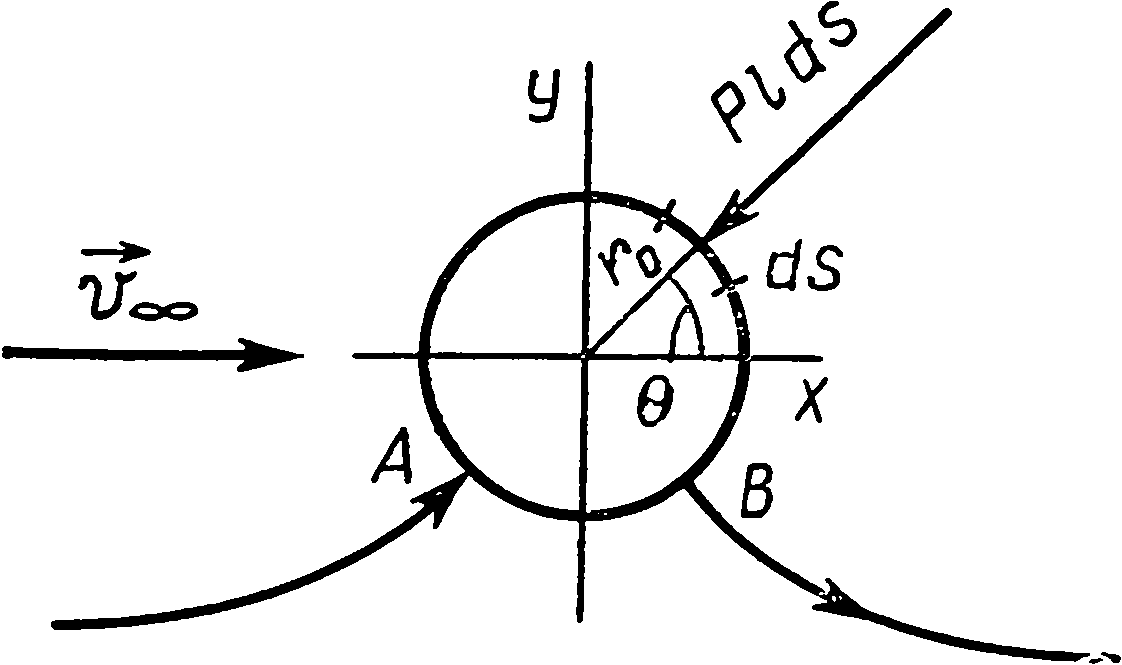
\includegraphics[width=0.35\linewidth]{img/circulating-cylinder-lifting-force-scheme}
		\caption{Схема для определения подъемной силы, возникающей при циркуляционном обтекании цилиндра.}
		\label{fig:7.9_circulating-cylinder-lifting-force-scheme}
	\end{figure}
	Вычислим значение подъемной силы, возникающей при обтекании цилиндра. Найдем сначала подъемную силу, действующую на элементарную площадку $l\dd s$ (здесь $l$ --- длина участка цилиндра вдоль его оси) в направлении оси $y$, т. е. в направлении перпендикуляра к вектору скорости невозмущенного потока $\bar{v}_\infty$ (\cref{fig:7.9_circulating-cylinder-lifting-force-scheme}). Она равна $\dd Y_\mathrm{a} = -pl\dd s\sin\varTheta$. Введем коэффициент давления $\bar{p}$. Тогда $p = p_\infty + \bar{p}\rho v_\infty^2/2$ и $\dd Y_\mathrm{a} = -\bar{p}\left(\rho v_\infty^2/2\right)l\dd s\sin\varTheta - p_\infty l\dd s\sin\varTheta$. 3дeсь $\dd s = r_0\dd\varTheta$. Тогда, интегрируя по углу $\varTheta$ от $0$ до $2\pi$ и имея в виду, что интеграл от второго члена равен нулю, получим суммарную подъемную силу:
	\begin{gather*}
		Y_\mathrm{a} = -\frac{\rho v_\infty^2}{2}lr_0\int\limits_0^{2\pi}\bar{p}\sin\varTheta\dd\varTheta.
	\end{gather*}\n
	Подставляя сюда выражение $\bar{p}$ \eqref{eq:731} и учитывая что $\int_0^{2\pi}\sin\varTheta\dd\varTheta = 0$, $\int_0^{2\pi}\sin^3\varTheta\dd\varTheta = 0$, $\int_0^{2\pi}\sin^2\varTheta\dd\varTheta = \pi$, получаем \textit{формулу Жуковского}:
	\begin{gather}\label{eq:732}
		Y_\mathrm{a} = \rho\Gamma v_\infty l.
	\end{gather}\n
	Итак, при безотрывном обтекании цилиндра установившимся потоком идеальной жидкости результирующая сила давления перпендикулярна вектору скорости набегающего потока. Значение ее не равно нулю только при циркуляции: $\Gamma \ne 0$.
	
	\subsection{Формула Чаплыгина о результирующей силе давления}
	Покажем, как непосредственно по комплексному потенциалу потока вычислить результирующую силу давления.\n
	В 1910 г. акад. С. А. Чаплыгин в своей известной работе «О давлении плоскопараллельного потока на преграждающие тела» дал общий прием определения результирующей силы и ее момента, создав основы теории крыла бесконечного размаха.\n
	Сущность метода Чаплыгина сводится к следующему. Допустим, что задан описываемый комплексным потенциалом $w = \varphi + i\psi$ плоский поток, плавно обтекающий цилиндрическое тело произвольной формы, ограниченное в плоскости $x$, $y$ контуром $L$.\n
	\begin{figure}[htbp]
		\centering
		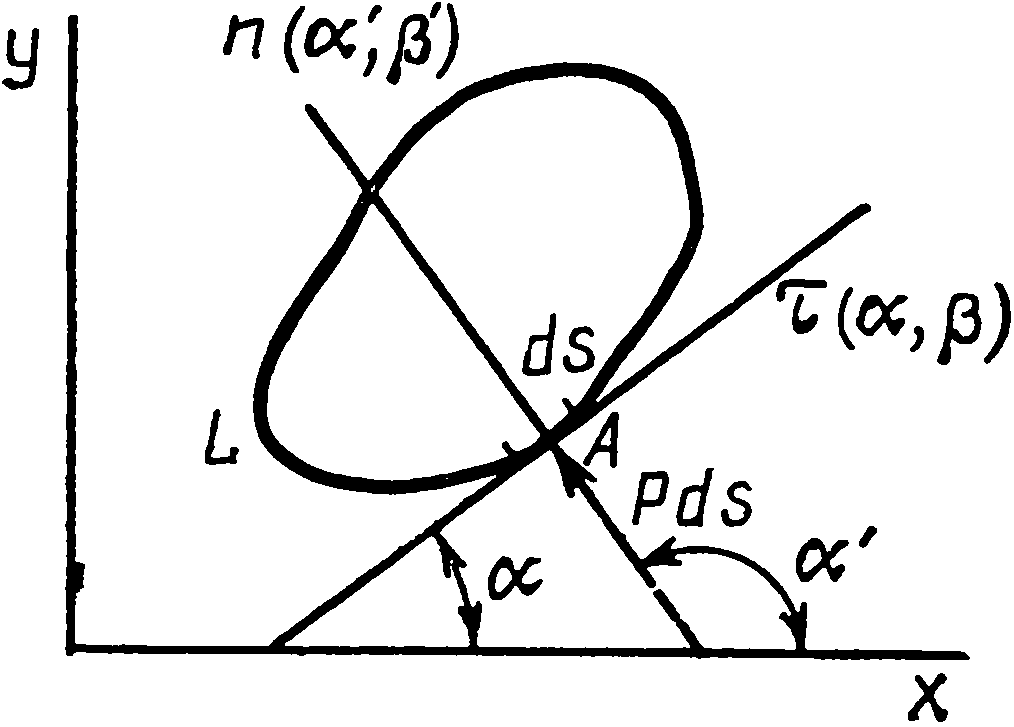
\includegraphics[width=0.3\linewidth]{img/scheme-for-Chaplygin-formulas}
		\caption{Схема для вывода формул Чаплыгина о результирующей силе давления и о моменте.}
		\label{fig:7.10_scheme-for-chaplygin-formulas}
	\end{figure}
	Рассмотрим на контуре произвольную точку $A$ (\cref{fig:7.10_scheme-for-chaplygin-formulas}). Проведем в ней касательную $\tau$ и нормаль $n$ к контуру. Обозначив $\alpha$ и $\beta$ углы, образуемые касательной с координатными осями, $\alpha'$ и $\beta'$ --- те же углы для нормали, получим:
	\begin{gather}\label{eq:733}
		\cos\alpha' = -\frac{\dd y}{\dd s} = -\sin\alpha;\quad
		\cos\beta' = +\frac{\dd x}{\dd s} = \cos\alpha.
	\end{gather}\n
	Давление $p$ в точке $A$ контура определим из уравнения Лагранжа-Бернулли
	\begin{gather*}
		p = C - \frac{\rho v^2}{2},
	\end{gather*}
	где $v$ --- скорость на контуре.\n
	Умножая элементарную силу давления $p\dd s$ в точке $A$ на $\cos\alpha'$ и $\cos\beta'$, найдем ее проекции на оси $x$ и $y'$. Проекции результирующей силы давления на координатные оси $X$ и $Y$, очевидно, выразятся в виде $X = \int_L p\dd s\cos\alpha'$, $Y = \int_L p\dd s\cos\beta'$, или в соответствии с формулой \eqref{eq:733}
	\begin{gather}\label{eq:734}
		X = -\int\limits_L p\sin\alpha\dd s;\quad
		Y = \int\limits_L p\cos\alpha\dd s.
	\end{gather}\n
	Используя формулы \eqref{eq:734} получаем
	\begin{gather*}
		Y + iX = \int\limits_L p\left(\cos\alpha - i\sin\alpha\right)\dd s.
	\end{gather*}
	Подставляя выражение для $p$ из уравнения Лагранжа-Бернулли, имеем
	\begin{gather*}
		Y + iX = \int\limits_L\left(C - \frac{\rho v^2}{2}\right)\left(\cos\alpha - i\sin\alpha\right)\dd s.
	\end{gather*}\n
	Здесь
	\begin{gather*}
		\int\limits_LC\cos\alpha\dd s = C\int\limits_L\frac{\dd x}{\dd s}\dd s = C\int\limits_L\dd x = 0;\\
		\int\limits_LC\sin\alpha\dd s = C\int\limits_L\frac{\dd y}{\dd s}\dd s = C\int\limits_L\dd y = 0,
	\end{gather*}
	так как координаты $x$ и $y$ при полном обходе по контуру принимают первоначальное значение. Тогда выражение для $Y + iX$ примет следующий вид:
	\begin{gather}\label{eq:735}
		Y + iX = -\frac{\rho}{2}\int\limits_L v^2\left(\cos\alpha - i\sin\alpha\right)\dd s.
	\end{gather}\n
	Преобразуем в формуле \eqref{eq:735} подынтегральное выражение. Так как на контуре скорость направлена по касательной, то $v = \frac{\dd\varphi}{\dd s}$ или $\dd\varphi = v\dd s$.\n
	Так как контур $L$ является линией тока, на которой $\psi = \mathrm{const}$, то, следовательно, на контуре $\dd w = \dd\left(\varphi + i\psi\right) = \dd\varphi$ и поэтому
	\begin{subequations}
		\begin{gather}\label{eq:124а}
			v\dd s = \dd w.
		\end{gather}\n
		Кроме того, на контуре $L$ для комплексной скорости $\frac{\dd w}{\dd z}$ имеем
		\begin{gather}\label{eq:125б}
			\frac{\dd w}{\dd z} = v_x - iv_y = v\left(\cos\alpha - i\sin\alpha\right).
		\end{gather}\n
	\end{subequations}
	При подстановке выражения \eqref{eq:124а} и \eqref{eq:125б} в формулу \eqref{eq:735}
	\begin{gather*}
		Y + iX = -\frac{\rho}{2}\int\limits_L\frac{\dd w}{\dd z}\dd w.
	\end{gather*}\n
	Но так как $\dd w = \frac{\dd w}{\dd z}\dd z$, то окончательно
	\begin{gather}\label{eq:736}
		Y + iX = -\frac{\rho}{2}\int\limits_L\left(\frac{\dd w}{\dd z}\right)^2\dd z.
	\end{gather}\n
	Это формула, позволяющая для потока, заданного комплексным потенциалом $w$, найти проекции $X$ и $Y$ результирующей силы давления по осям координат, называется \textit{формулой Чаплыгина}.\n
	Полная сила давления при этом равна $R = \sqrt{X^2 + Y^2}$. Заметим, что здесь $X$, $Y$ --- силы, действующие на единицу длины тела в направлении оси, перпендикулярной к плоскости $x$, $y$.
	
	\subsection{Формула Чаплыгина о моменте результирующей силы давления}
	Для определения аэродинамических характеристик важно знать не только значение результирующей силы давления потока на тело, но и точку ее приложения, называемую \textit{центром давления}, который будет известен, если подсчитать момент результирующей силы давления.\n
	По формуле Чаплыгина можно вычислить момент результирующей силы давления, зная комплексный потенциал потока. Для нахождения момента $M$ результирующей силы давления относительно начала координат поступим следующим образом.\n
	Представим момент $\dd M$ элементарной силы давления $p\dd s$ (\cref{fig:7.10_scheme-for-chaplygin-formulas}) относительно начала координат в следующем виде: $\dd M = p\left(x\cos\beta' - y\cos\alpha'\right)\dd s$. Результирующий момент сил давления, очевидно, получится, если мы от этого выражения возьмем интеграл по замкнутому контуру $L$ тела:
	\begin{gather}\label{eq:737}
		M = \int\limits_L p\left(x\cos\alpha + y\sin\alpha\right)\dd s.
	\end{gather}\n
	Подставим в этот интеграл выражение для давления $p$ из уравнения Лагранжа-Бернулли $p = C - \frac{\rho v^2}{2}$. Тогда
	\begin{gather*}
		M = \int\limits_L\left(C - \frac{\rho v^2}{2}\right)\left(x\cos\alpha + y\sin\alpha\right)\dd s,
	\end{gather*}
	или
	\begin{gather*}
		M = C\int\limits_L\left(x\cos\alpha + y\sin\alpha\right)\dd s - \frac{\rho}{2}\int\limits_L v^2\left(x\cos\alpha + y\sin\alpha\right)\dd s.
	\end{gather*}\n
	Покажем, что первый интеграл равен нулю:
	\begin{gather*}
		\int\limits_L\left(x\cos\alpha + y\sin\alpha\right)\dd s = \int\limits_L\left(x\frac{\dd x}{\dd s} + y\frac{\dd y}{\dd s}\right)\dd s = \int\limits_L x\dd x + y\dd y = \int\limits_L\dd\left(\frac{x^2 + y^2}{2}\right) = 0,
	\end{gather*}
	так как при полном обходе контура $L$ координаты $x$ и $y$ приобретают первоначальные значения. Следовательно, выражение для момента $M$ принимает следующий вид:
	\begin{gather}\label{eq:738}
		M = -\frac{\rho}{2}\int\limits_L v^2\left(x\cos\alpha + y\sin\alpha\right)\dd s.
	\end{gather}\n
	Для преобразования подынтегрального выражения вычислим произведение:
	\begin{gather}
		z\frac{\dd w}{\dd z} = \left(x + iy\right)\left(v_x - iv_y\right) = \left(xv_x + yv_y\right) + i\left(yv_x - xv_y\right).
	\end{gather}\n
	Вводя обозначения $xv_x + yv_y = m$, $yv_x - xv_y = n$, получаем
	\begin{subequations}
		\begin{gather}\label{eq:126а}
			z\frac{\dd w}{\dd z} = m + in.
		\end{gather}\n
		Вычислим теперь произведение $\frac{\dd w}{\dd z}\dd z$:
		\begin{gather*}
			\frac{\dd w}{\dd z}\dd z = \left(v_x - iv_y\right)\left(\dd x + i\dd y\right) = \left(v_x\dd x + v_y\dd y\right) + i\left(v_x\dd y - v_y\dd x\right).
		\end{gather*}\n
		Так как $v_x\dd x + v_y\dd y = \dd\varphi$, $v_x\dd y - v_y\dd x = \dd\psi$ и на контуре $L$, являющемся линией тока, $\dd\psi = 0$, $\dd\varphi = v\dd s$, то
		\begin{gather}\label{eq:126б}
			\frac{\dd w}{\dd z}\dd z = v\dd s.
		\end{gather}\n
		Перемножаем выражение \eqref{eq:126а} и \eqref{eq:126б}:
		\begin{gather}\label{eq:126в}
			z\left(\frac{\dd w}{\dd z}\right)^2\dd z = v\left(m + in\right)\dd s.
		\end{gather}\n
		Так как $m = xv_x + yv_y = v\left(x\cos\alpha + y\sin\alpha\right)$, $n = yv_x - xv_y = v\left(y\cos\alpha - x\sin\alpha\right)$, то соотношение \eqref{eq:126в} можно представить в следующем виде:
		\begin{gather*}
			z\left(\frac{\dd w}{\dd z}\right)^2\dd z = v^2\left(x\cos\alpha + y\sin\alpha\right)\dd s + iv^2\left(y\cos\alpha - x\sin\alpha\right)\dd s,
		\end{gather*}
		т. е. $v^2\left(x\cos\alpha + y\sin\alpha\right)\dd s = \mathrm{Reel}\left[z\left(\frac{\dd w}{\dd z}\right)^2\dd z\right]$.\n
	\end{subequations}
	Подставляя это выражение в \eqref{eq:738}, окончательно находим
	\begin{gather}\label{eq:739}
		M = -\mathrm{Reel}\left[\frac{\rho}{2}\int\limits_L z\left(\frac{\dd w}{\dd z}\right)^2\dd z\right].
	\end{gather}\n
	Формулу \eqref{eq:739} называют \textit{формулой Чаплыгина}, которая позволяет для заданного комплексным потенциалом $w$ потока вычислить результирующий момент $M$ силы давления.\n
	В качестве примера, иллюстрирующего применение выведенных формул \eqref{eq:736} и \eqref{eq:739}, рассмотрим циркуляционное обтекание цилиндра. В этом случае комплексный потенциал определяется по формуле \eqref{eq:728}. Дифференцируя $w$ по $z$, т. е. $\frac{\dd w}{\dd z} = v_\infty\left(1 - r_0^2/z^2\right) + \frac{i\Gamma/2\pi}{z}$, и подставляя найденное значение $\frac{\dd w}{\dd z}$ в формулу Чаплыгина \eqref{eq:736}, получаем
	\begin{gather*}
		Y + iX = -\frac{\rho}{2}\int\limits_L\left[v_\infty^2\left(1 - \frac{r_0^2}{z^2}\right)^2 + \left(1 - \frac{r_0^2}{z^2}\right)\frac{iv_\infty\Gamma}{\pi}\frac{1}{z} - \frac{\Gamma^2}{4\pi^2}\frac{1}{z^2}\right]\dd z.
	\end{gather*}\n
	Вычет относительно полюса $z = 0$ даст лишь член, содержащий $1/z$, т. e. $\frac{iv_\infty\Gamma/\pi}{z}$. В таком случае
	\begin{gather*}
		Y + iX = -\frac{\rho}{2}2\pi i\frac{v_\infty i\Gamma}{\pi}, \hspace{0.5em} \mathrm{или} \hspace{0.5em} Y + iX = \rho v_\infty\Gamma,
	\end{gather*}
	откуда $X = 0$, $Y = \rho v_\infty\Gamma$.\n
	Поскольку в рассматриваемой задаче обтекания цилиндра направление оси $x$ совпадает с направлением скорости невозмущенного потока, то $X = X_\mathrm{a}$, $Y = Y_\mathrm{a}$, т. е. полученный результат означает, что при этом лобовое сопротивление отсутствует $\left(X_\mathrm{a} = 0\right)$, а подъемная сила, отнесенная к единице длины цилиндра $\left(l = 1\right)$, определяется по известной формуле Жуковского $Y_\mathrm{a} = \rho v_\infty\Gamma$ [см. формулу \eqref{eq:732}].\n
	Для нахождения момента $M$ результирующей силы давления, действующей на цилиндр, используем формулу \eqref{eq:739}. Подставим в нее выражение $z\left(\frac{\dd w}{\dd z}\right)^2$. Тогда
	\begin{gather*}
		M = \mathrm{Reel}\left\{\frac{\rho}{2}2\pi i\left[\frac{\Gamma^2}{4\pi^2} + 2v_\infty^2 r_0^2\right]\right\}.
	\end{gather*}\n
	Так как выражение в фигурных скобках представляет собой чисто мнимую величину, то $M = 0$, т. е. в этом случае результирующая сила $Y_\mathrm{a}$ проходит через ось цилиндра.
	
	\subsection{Тонкий профиль крыла в несжимаемом потоке. Теория тонкого профиля}\label{sec:incompressible-flow-thin-profile}
	\begin{figure}[htbp]
		\centering
		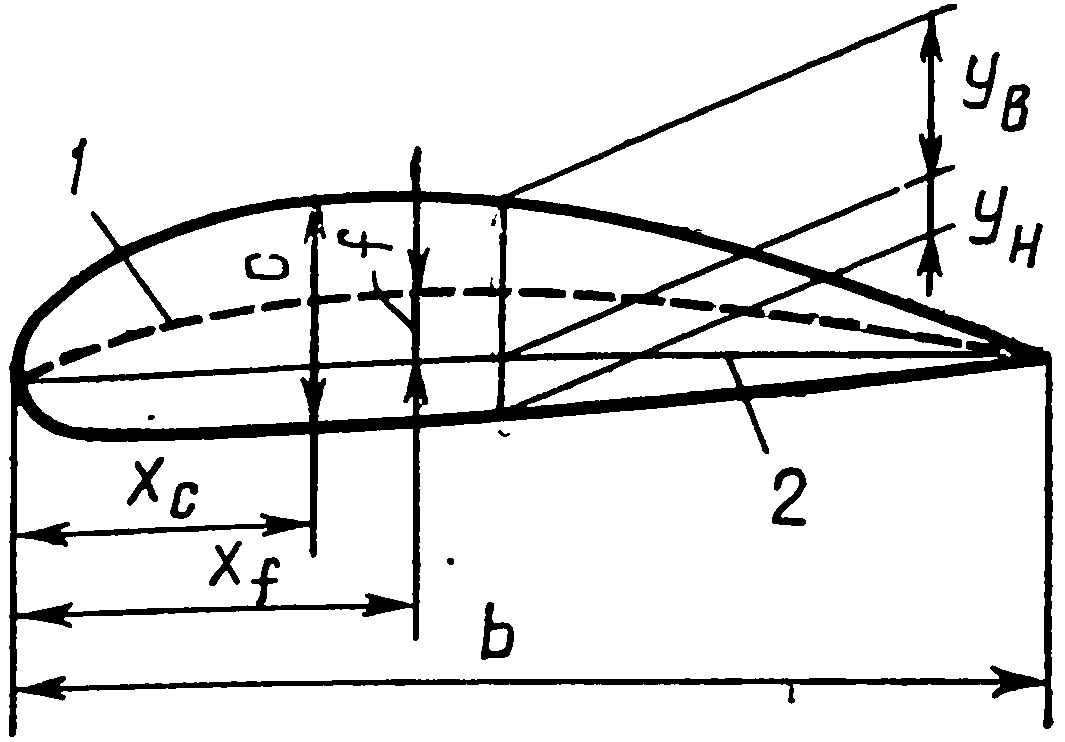
\includegraphics[width=0.3\linewidth]{img/thin-profile-geometric-characteristics}
		\caption{Геометрические характеристики тонкого профиля:\\\small{\textit{1} --- средняя линия; \textit{2} --- хорда.}}
		\label{fig:7.11_thin-profile-geometric-characteristics}
	\end{figure}
	Профиль крыла представляет собой контур сечения крыла бесконечного размаха плоскостью, перпендикулярной его размаху. Для характеристики формы этого профиля (\cref{fig:7.11_thin-profile-geometric-characteristics}) рассмотрим его основные геометрические параметры.\n
	Линией, относительно которой определяются координаты верхней и нижней плоскостей профиля $y_\mathrm{в}$ и $y_\mathrm{н}$, является его хорда. \textit{Хорда} $b$ --- это отрезок прямой, соединяющий две наиболее удаленные точки профиля (переднюю и заднюю кромки). Обычно координаты профиля определяются в долях хорды $\bar{y}_\mathrm{в} = y_\mathrm{в}/b$, $\bar{y}_\mathrm{н} = y_\mathrm{н}/b$. Толщина профиля в данной точке равна длине перпендикулярного хорде отрезка, соединяющего точки верхнего и нижнего контуров профиля. Обычно под толщиной профиля $c$ понимают его максимальную толщину. Одним из основных геометрических параметров профиля является относительная толщина профиля: $\bar{c} = c/b$. Форму профиля определяет также расстояние $x_c$ от его передней кромки до точки на хорде, в которой профиль имеет максимальную толщину. Это расстояние также определяется в долях хорды: $\bar{x}_c = x_c/b$.\n
	В значительной степени форму профиля определяет его \textit{средняя линия} --- линия, соединяющая точки, расположенные посередине толщин профиля. Расстояние от хорды до средней линии называется \textit{вогнутостью}. Максимальная вогнутость $f$, выражаемая в долях хорды, называется относительной вогнутостью или относительной кривизной профиля. Расстояние от передней кромки профиля до точки на хорде, соответствующей максимальной вогнутости, обозначается $x_f$, а в долях хорды $\bar{x}_f = x_f/b$. Для симметричного профиля средняя линия совпадает с хордой и $f = 0$.\n
	В \cref{sec:7.2} рассмотрена задача обтекания контура в виде круга (сечения круглого цилиндра). Задача об обтекании профиля произвольной формы решается до конца, если известно конформное преобразование внешности этого профиля на внешность круга. Однако отыскание такого конформного преобразования в явном виде для профиля произвольной формы связано с большими трудностями.\n
	Классические работы Н. Е. Жуковского и С. А. Чаплыгина по теоретическим профилям, основанные на введении отображающих функций, дали возможность построить точное решение для ограниченного класса профилей. Поэтому представляют интерес приближенные методы решения задачи обтекания профилей произвольной формы. Наибольшее применение при определении аэродинамических характеристик профиля находят результаты теории тонкого профиля, основанной на замене профиля системой простых особенностей в виде присоединенных вихрей. Рассмотрим обтекание тонкого слабоизогнутого профиля под малым углом атаки $\alpha$ установившимся потоком невязкой несжимаемой среды с заданной скоростью $v_\infty$.\n
	\begin{figure}[htbp]
		\centering
		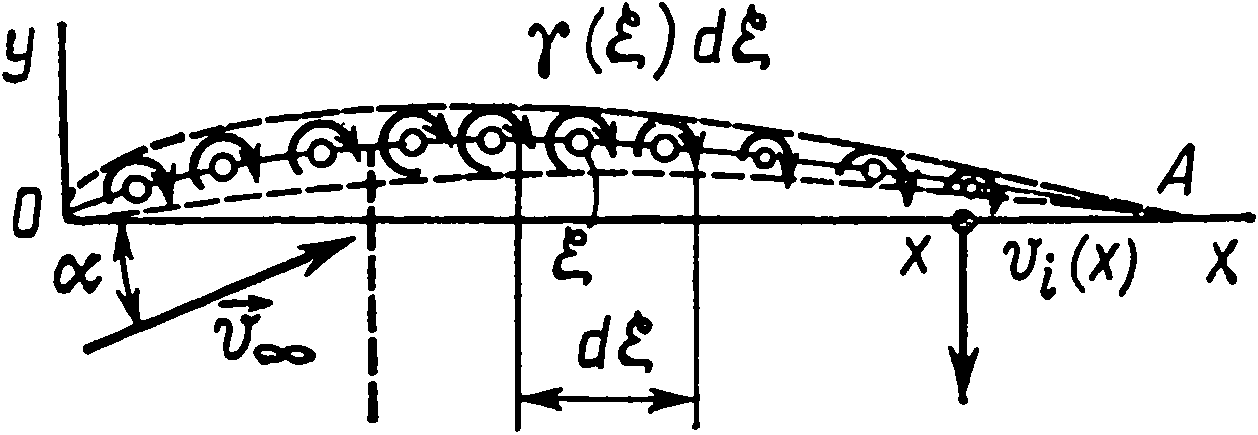
\includegraphics[width=0.3\linewidth]{img/thin-profile-in-incompressible-flow}
		\caption{Тонкий профиль в несжимаемом потоке.}
		\label{fig:7.12_thin-profile-in-incompressible-flow}
	\end{figure}
	Поместим начало координат в передней кромке профиля, ось $x$ направим вдоль хорды, ось $y$ --- перпендикулярно ей вверх (\cref{fig:7.12_thin-profile-in-incompressible-flow}). Введем следующие упрощения:
	\begin{enumerate}
		\item предполагая профиль достаточно тонким, считаем, что он мало отличается от своей средней линии, и рассмотрим вместо профиля обтекание его средней линии;
		\item предполагая профиль слабоизогнутым, принимаем, что средняя линия незначительно отличается от хорды профиля;
		\item рассматривая обтекание тонкого слабоизогнутого профиля под малым углом атаки, считаем, что обтекание безотрывно, т. е. средняя линия является линией тока.
	\end{enumerate}\n
	Затем заменим профиль непрерывно расположенными по его средней линии вихрями бесконечного размаха с осями вращения вдоль оси $z$ (вдоль перпендикуляра к плоскости $xy$).\n
	Возможность такой замены подтверждается следующими соображениями. Согласно формуле Жуковского \eqref{eq:732}, подъемная сила профиля $Y_\mathrm{a} \ne 0$, если циркуляция скорости по контуру $L$, охватывающему профиль, отлична от нуля: $\Gamma \ne 0$. С другой стороны, на основании теоремы Стокса о вихрях условие $\Gamma \ne 0$ означает, что область, ограниченная контуром $L$, пронизывается вихрями с суммарной интенсивностью, равной циркуляции $\Gamma$. Отсюда следует, что профиль по своему воздействию на обтекающий его поток эквивалентен вихрям. Эти вихри называются \textit{присоединенными}.\n
	Обозначим $\gamma\left(x\right)$ погонную циркуляцию скорости:
	\begin{gather*}
		\gamma\left(x\right) = \lim_{\Delta x\to 0}\frac{\Delta\Gamma}{\Delta x}.
	\end{gather*}
	Здесь $\Delta\Gamma$ --- циркуляция скорости от вихрей, расположенных на элементе $\Delta x$ средней линии. Функцию $\gamma\left(x\right)$ следует подобрать из условия, что средняя линия профиля является линией тока. Напомним, что в случае круглого цилиндра достаточно ввести один присоединенный вихрь, расположенный вдоль его оси.\n
	Вектор скорости в окрестности профиля и на его средней линии можно представить в виде суммы: $\vv{v} = \vv{v}_\infty + \vv{v}_i$, где $\vv{v}_i$ --- вектор скорости, индуцированной в данной точке присоединенными вихрями. Для тонкого профиля примем, что вихри расположены вдоль хорды, а не на его средней линии. По формуле Био-Савара \eqref{eq:237}, скорость, индуцированная элементом с циркуляцией $\dd\Gamma = \gamma\left(\xi\right)\dd\xi$ в некоторой точке хорды с координатой $x$, равна $\dd v_i = \frac{\gamma\left(\xi\right)\dd\xi}{2\pi\left(x - \xi\right)}$. Здесь за положительное направление скорости $v_i$ принято направление вниз. Тогда скорость, индуцированная в этой точке всеми вихрями,
	\begin{gather}\label{eq:740}
		v_i\left(x\right) = \frac{1}{2\pi}\int\limits_0^b\frac{\gamma\left(\xi\right)\dd\xi}{x - \xi}.
	\end{gather}\n
	Эту индуцированную скорость $v_i\left(x\right)$ на хорде профиля можно принять равной индуцированной скорости на поверхности профиля. Наличие этой скорости изменяет угол атаки в данной точке на величину $\Delta\alpha = v_i\left(x\right)/v_\infty$. При этом местный угол атаки будет $\alpha - v_i\left(x\right)/v_\infty$.\n
	Для того чтобы профиль обтекался безотрывно, необходимо, чтобы в каждой его точке местная скорость была направлена по касательной к поверхности, т. е. должно быть равенство
	\begin{gather}\label{eq:741}
		\alpha - \frac{v_i}{v_\infty} = \frac{\dd y}{\dd x},
	\end{gather}
	где $y = y\left(x\right)$ --- уравнение средней линии профиля.\n
	Используя выражение \eqref{eq:740} для $v_i$, равенство \eqref{eq:741} можно представить в следующем виде:
	\begin{gather}\label{eq:742}
		\alpha - \frac{1}{2\pi v_\infty}\int\limits_0^b\frac{\gamma\left(\xi\right)\dd\xi}{x - \xi} = \frac{\dd y}{\dd x}.
	\end{gather}\n
	Уравнение \eqref{eq:742} --- интегральное уравнение относительно неизвестной функции $\gamma\left(\xi\right)$. Введем вместо $x$ и $\xi$ новые независимые переменные $\varTheta_1$ и $\varTheta$, определяемые равенствами $x = \left(b/2\right)\left(1 - \cos\varTheta_1\right)$, $\xi = \left(b/2\right)\left(1 - \cos\varTheta\right)$. Очевидно, когда $x$ и $\xi$ изменяются в пределах $0 \leqslant x \leqslant b$, $0 \leqslant \xi \leqslant b$, переменные $\varTheta_1$ и $\varTheta$ изменяются в пределах $0 \leqslant \varTheta_1 \leqslant \pi$, $0 \leqslant \varTheta \leqslant \pi$.\n
	Будем искать $\gamma\left(\varTheta\right)$ в виде ряда
	\begin{gather}\label{eq:743}
		\gamma\left(\varTheta\right) = 2v_\infty\left[A_0\ctg\frac{\varTheta}{2} + \sum_{n = 1}^{\infty}A_n\sin n\varTheta\right],
	\end{gather}
	коэффициенты которого $A_0$, $A_1$, $A_2$, $\dots$ должны быть подобраны так, чтобы удовлетворялось условие безотрывности обтекания, т. е. уравнение \eqref{eq:742}. Для этого прежде всего приведем выражение \eqref{eq:740} и уравнение \eqref{eq:742} к переменному $\varTheta$:
	\begin{gather}\label{eq:744}
		v_i = \frac{1}{2\pi}\int\limits_0^b\frac{\gamma\left(\xi\right)\dd\xi}{x - \xi} = \frac{1}{2\pi}\int\limits_0^\pi\frac{\gamma\left(\varTheta\right)\sin\varTheta\dd\varTheta}{\cos\varTheta - \cos\varTheta_1}.
	\end{gather}\n
	Найдем теперь выражение $\gamma\left(\varTheta\right)\sin\varTheta$:
	\begin{gather*}
		\begin{aligned}
			\gamma\left(\varTheta\right)\sin\varTheta &= 2v_\infty\left(A_0\ctg\frac{\varTheta}{2} + \sum_{n = 1}^{\infty}A_n\sin n\varTheta\right)\sin\varTheta =\\
			&= 2v_\infty\left[A_0\left(1 + \cos\varTheta\right) + \sum_{n=1}^{\infty}A_n\sin n\varTheta\sin\varTheta\right] =\\
			&=2v_\infty\left[A_0\left(1 + \cos\varTheta\right) + \sum_{n=1}^{\infty}A_n\frac{\cos\left(n-1\right)\varTheta-\cos\left(n+1\right)\varTheta}{2}\right].
		\end{aligned}
	\end{gather*}\n
	Подставляя полученное выражение в формулу \eqref{eq:744}, имеем
	\begin{gather}\label{eq:745}
		\begin{aligned}
			v_i = \frac{v_\infty}{\pi}\int\limits_0^\pi\frac{A_0\dd\varTheta}{\cos\varTheta-\cos\varTheta_1} &+ \frac{v_\infty}{\pi}\int\limits_0^\pi\frac{A_0\cos\varTheta\dd\varTheta}{\cos\varTheta-\cos\varTheta_1} +\\
			&+ \frac{v_\infty}{2\pi}\int\limits_0^\pi\sum_{n=1}^{\infty}A_n\frac{\cos\left(n-1\right)\varTheta-\cos\left(n+1\right)\varTheta}{\cos\varTheta-\cos\varTheta_1}\dd\varTheta.
		\end{aligned}
	\end{gather}\n
	Так как
	\begin{gather*}
		\int\limits_0^\pi\frac{\dd\varTheta}{\cos\varTheta-\cos\varTheta_1} = 0,\quad
		\int\limits_0^\pi\frac{\cos k\varTheta\dd\varTheta}{\cos\varTheta-\cos\varTheta_1} = \pi\frac{\sin k\varTheta_1}{\sin\varTheta_1},
	\end{gather*}
	то, подставляя значения этих интегралов в формулу \eqref{eq:745}, после некоторых преобразований получаем
	\begin{gather}\label{eq:746}
		v_i = v_\infty\left[A_0-\sum_{n=1}^{\infty}A_n\cos n\varTheta_1\right].
	\end{gather}\n
	Теперь уравнение \eqref{eq:742} можно представить в следующем виде:
	\begin{gather}\label{eq:747}
		\alpha-A_0+\sum_{n=1}^{\infty}A_n\cos n\varTheta=\frac{\dd y}{\dd x}.
	\end{gather}
	Коэффициенты $A_n$ этого уравнения определяются методом, обычным для рядов Фурье. Умножая обе части уравнения \eqref{eq:747} поочередно на 1, $\cos\varTheta$, $\cos 2\varTheta$, $\cos 3\varTheta$, $\dots$ и интегрируя в пределах от 0 до $\pi$, получаем:
	\begin{gather}\label{eq:748}
		A_0=\alpha-\frac{1}{\pi}\int\limits_0^\pi\frac{\dd y}{\dd x}\dd\varTheta;\quad
		A_n=\frac{2}{\pi}\int\limits_0^\pi\frac{\dd y}{\dd x}\cos n\varTheta\dd\varTheta,
	\end{gather}
	где $y\left(x\right)$ выражено через $\varTheta$ с помощью подстановки $x=\left(b/2\right)\left(1-\cos\varTheta\right)$.\n
	В случае симметричного профиля $y=0$, $\frac{\dd y}{\dd x}=0$ и $A_0=\alpha$, $A_1=A_2=\dots=0$. Тогда $\gamma=2v_\infty\alpha\ctg\varTheta/2$. Отсюда очевидно, что при удалении от передней кромки профиля интенсивность присоединенных вихрей уменьшается. На задней кромке $\left(\varTheta=\pi\right)$ $\gamma=0$.\n
	Зная распределение интенсивности присоединенных вихрей по хорде, легко найти подъемную силу и момент, действующие на профиль. По теореме Жуковского, $\dd Y_\mathrm{a}=\rho\gamma\left(x\right)v_\infty l\dd x$ и, следовательно,
	\begin{gather*}
		Y_\mathrm{a}=\rho v_\infty l\int\limits_0^b\gamma\left(x\right)\dd x.
	\end{gather*}\n
	Переходя к переменному $\varTheta$, получаем
	\begin{gather*}
		Y_\mathrm{a}=\rho v_\infty^2 lb\int\limits_0^\pi\left[A_0\left(1+\cos\varTheta\right)+\sum_{n=1}^{\infty}A_n\sin n\varTheta\sin\varTheta\right]\dd\varTheta = \rho v_\infty^2 lb\left(A_0+\frac{A_1}{2}\right)\pi,
	\end{gather*}
	откуда коэффициент подъемной силы
	\begin{gather}\label{eq:749}
		c_{ya}=2\pi\left(A_0+\frac{A_1}{2}\right).
	\end{gather}\n
	Аналогично вычисляется момент относительно передней кромки профиля:
	\begin{gather*}
		M=-\rho v_\infty l\int\limits_0^b\gamma\left(x\right)x\dd x.
	\end{gather*}\n
	Переходя к переменной $\varTheta$, имеем
	\begin{gather*}
		\begin{aligned}
			\rho v_\infty l\gamma\left(x\right)x\dd x &= v_\infty^2 l\frac{b^2}{2}\left[A_0\left(1-\cos^2\varTheta\right)+\left(1-\cos\varTheta\right)\sum_{n=1}^{\infty}A_n\sin n\varTheta\sin\varTheta\right]\dd\varTheta =\\
			&= v_\infty^2 l\frac{b^2}{2}\left[A_0\frac{1-\cos 2\varTheta}{2}+\sum_{n=1}^{\infty}A_n\sin n\varTheta\left(\sin\varTheta-\frac{\sin 2\varTheta}{2}\right)\right]\dd\varTheta.
		\end{aligned}
	\end{gather*}\n
	Тогда
	\begin{gather*}
		\begin{aligned}
			M&=-\frac{\rho v_\infty^2}{2}lb^2\left[\int\limits_0^\pi A_0\frac{1-\cos 2\varTheta}{2}\dd\varTheta+\int\limits_0^\pi\sum_{n=1}^{\infty}A_n\sin n\varTheta\left(\sin\varTheta-\frac{\sin 2\varTheta}{2}\right)\dd\varTheta\right] =\\
			&=-\frac{\rho v_\infty^2}{2}lb^2\frac{\pi}{2}\left(A_0+A_1-\frac{A_2}{2}\right).
		\end{aligned}
	\end{gather*}\n
	Отсюда коэффициент момента
	\begin{gather}\label{eq:750}
		c_m=-\frac{\pi}{2}\left(A_0+A_1-\frac{A_2}{2}\right).
	\end{gather}\n
	Как видим, значения подъемной силы и момента определяются лишь первыми тремя коэффициентами разложения: $A_0$, $A_1$ и $A_2$; остальные коэффициенты не влияют на суммарные аэродинамические характеристики (подъемную силу и момент), но влияют на распределение $\gamma\left(x\right)$.\n
	Подставляя в формулы \eqref{eq:749} и \eqref{eq:750} выражения \eqref{eq:748}, получаем:
	\begin{gather}
		c_{ya}=2\pi\left(\alpha-\alpha_0\right);\label{eq:751}\\
		c_m=c_{m0}-\frac{c_{y\mathrm{a}}}{4},\label{eq:752}
	\end{gather}
	где
	\begin{gather}\label{eq:753}
		\begin{dcases}
			\alpha_0=\frac{1}{\pi}\int\limits_0^\pi\frac{\dd y}{\dd x}\left(1-\cos\varTheta\right)\dd\varTheta;\\
			c_{m0}=-\frac{1}{2}\int\limits_0^\pi\frac{\dd y}{\dd x}\left(\cos\varTheta-\cos 2\varTheta\right)\dd\varTheta.
		\end{dcases}
	\end{gather}\n
	Угол $\alpha_0$ называется \textit{углом атаки} нулевой подъемной силы, т. е. при $\alpha=\alpha_0$, эта сила равна нулю.\n
	Из формулы для $c_{y\mathrm{a}}$ следует, что для тонких профилей коэффициент подъемной силы линейно зависит от угла атаки $\alpha$, а производная $c_{y\mathrm{a}}^\alpha=2\pi$ не зависит от формы профиля. Коэффициент $c_{m0}$ равен коэффициенту момента при нулевой подъемной силе.\n
	Из формулы \eqref{eq:753} следует, что величины $\alpha_0$ и $c_{m0}$ зависят только от формы средней линии профиля (от вогнутости). Для симметричных профилей $\alpha_0=0$, $c_{m0}=0$. При увеличении относительной вогнутости профиля $\alpha_0$ и $c_{m0}$ по абсолютной величине увеличиваются.\n
	При малых углах атаки зависимость коэффициента момента от коэффициента подъемной силы (угла атаки), так же как зависимость $c_{y\mathrm{a}}$ от $\alpha$, линейна [см. \eqref{eq:752}]. Однако при больших углах атаки безотрывность обтекания профиля нарушается --- происходит отрыв потока (см. \cref{prt:boundary-layer}). При этом зависимости $c_{y\mathrm{a}}\left(\alpha\right)$ и $c_m\left(\alpha\right)$ становятся нелинейными.\n
	\begin{figure}[htbp]
		\centering
		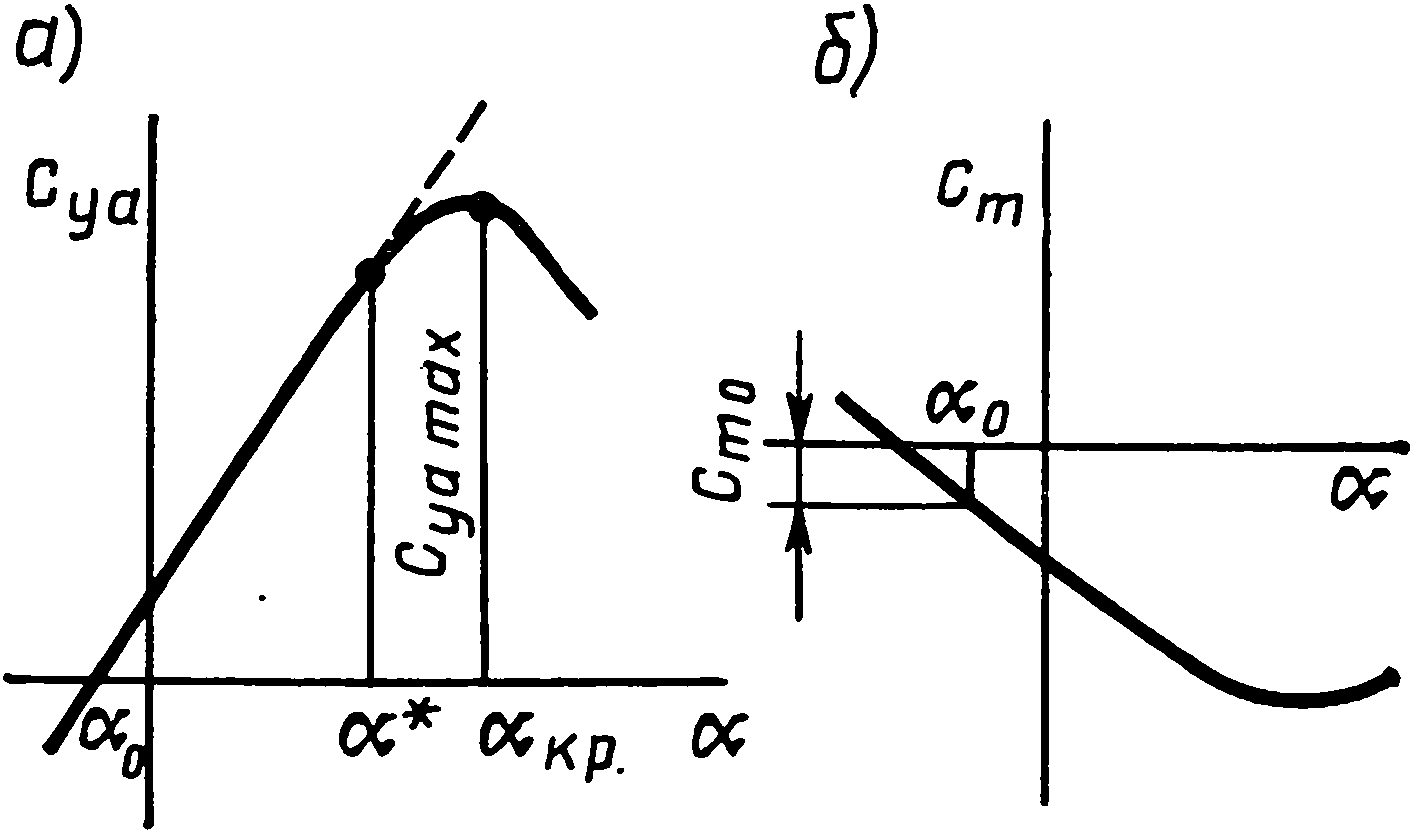
\includegraphics[width=0.35\linewidth]{img/cya-and-cm-vs-alpha}
		\caption{Зависимости коэффициентов подъемной силы \textit{(а)} и момента \textit{(б)} от угла атаки.}
		\label{fig:7.13_cya-and-cm-vs-alpha}
	\end{figure}
	На \cref{fig:7.13_cya-and-cm-vs-alpha} приведен типичный характер зависимости коэффициентов $c_{y\mathrm{a}}$ и $c_m$ от угла атаки для несимметричного профиля. Здесь $\alpha_\mathrm{кр}$ --- критический угол атаки, при котором коэффициент подъемной силы имеет максимальное значение $c_{y\mathrm{a}}$ = $c_{y\mathrm{a\,max}}$, а диапазон углов атаки $\alpha\leqslant\alpha^*$ соответствует безотрывному обтеканию профиля с линейным характером зависимости коэффициента $c_{y\mathrm{a}}$ от $\alpha$. При малых углах атаки теоретические результаты удовлетворительно согласуются с опытными данными. Опыт подтверждает, что кривизна профиля не влияет на значения производных $c_{y\mathrm{a}}^\alpha$ и $c_m^\alpha$. Однако теория дает завышенные значения производной $c_{y\mathrm{a}}^\alpha$, так как на величину $c_{y\mathrm{a}}^\alpha$ влияет относительная толщина профиля. С увеличением относительной толщины $\bar{c}$ производная $c_{y\mathrm{a}}^\alpha$ уменьшается.\n
	На значения коэффициента $c_{m0}$ и угла $\alpha_0$ существенно влияет кривизна профиля [см. \eqref{eq:753}]. При этом теория дает завышенные значения $c_{m0}$ и $\alpha_0$. Относительная толщина на $c_{m0}$ и $\alpha_0$ практически не влияет.\n
	Введем понятия о центре давления и фокусе профиля.\n
	\textit{Центром давления} называется точка на хорде профиля, через которую проходит равнодействующая аэродинамической силы.\n
	\textit{Фокусом профиля} называется точка на хорде, относительно которой (или относительно оси, проходящей через эту точку) момент не зависит от угла атаки.\n
	Обозначим $\bar{x}_\mathrm{д}$ и $\bar{x}_F$ соответственно относительные координаты центра давления и фокуса. Для определения координат центра давления и фокуса приведем выражение момента $M\left(x\right)$ относительно произвольной точки на хорде: $M\left(x\right)=M+Yx$, где $M$ --- момент относительно передней кромки; $x$ --- координата рассматриваемой точки. Отсюда коэффициент момента $c_m\left(\bar{x}\right)=c_m+c_{y\mathrm{a}}\bar{x}$· Подставляя сюда выражение \eqref{eq:752}, находим
	\begin{gather}\label{eq:754}
		c_m\left(\bar{x}\right)=c_{m0}+\left(\bar{x}-\frac{1}{4}\right)c_{y\mathrm{a}}.
	\end{gather}
	Здесь при малых углах атаки $c_y=c_{y\mathrm{a}}$.\n
	Для центра давления, т. е. при $\bar{x}=\bar{x}_\mathrm{д}$, коэффициент $c_m\left(\bar{x}\right)=0$, тогда, используя выражение \eqref{eq:754}, получим
	\begin{gather}\label{eq:755}
		\bar{x}_\mathrm{д}=\frac{1}{4}-\frac{c_{m0}}{c_{y\mathrm{a}}}.
	\end{gather}\n
	Из формулы \eqref{eq:755} следует, что для симметричных профилей независимо от формы $\bar{x}_\mathrm{д}=1/4$. В случае несимметричных профилей относительная координата центра давления зависит от формы профиля и коэффициента подъемной силы $c_{y\mathrm{a}}$ (угла атаки). При увеличении угла атаки центр давления смещается к передней кромке.\n
	Поскольку относительно фокуса момент не зависит от угла атаки, то из выражения \eqref{eq:754} следует, что при $\bar{x}=\bar{x}_F$
	\begin{gather}\label{eq:756}
		\left(\bar{x}_F-\frac{1}{4}\right)c_y=0, \hspace{0.5em} \text{т. е.} \hspace{0.5em} \bar{x}_F = \frac{1}{4}.
	\end{gather}\n
	Таким образом, фокус тонкого профиля независимо от формы располагается на расстоянии 1/4 хорды от передней кромки.\n
	\begin{figure}[htbp]
		\centering
		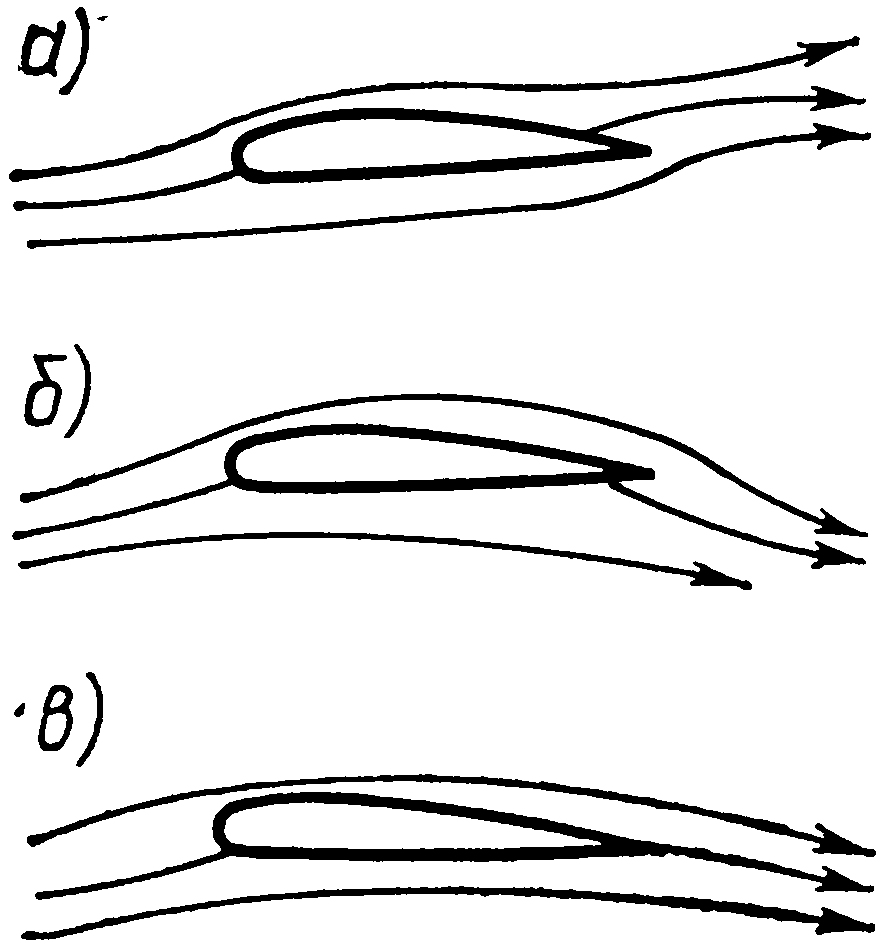
\includegraphics[width=0.2\linewidth]{img/profile-circulation-flow-patterns}
		\caption{Различные схемы циркуляционного обтекания профиля.}
		\label{fig:7.14_profile-circulation-flow-patterns}
	\end{figure}
	Рассмотрим еще одну существенную особенность обтекания профилей. При обтекании цилиндра с заданной скоростью на бесконечности $v_\infty$ имеется много решений, так как, выбирая разную циркуляцию $\Gamma$, можно получить различный характер обтекания цилиндра с различным расположением на нем критических точек [см. \eqref{eq:730}]. Это наблюдается и для профиля с острой задней кромкой. При обтекании профиля с заданной скоростью $v_\infty$ из бесчисленного множества решений можно выделить три случая, отличающихся характером обтекания задней кромки профиля (\cref{fig:7.14_profile-circulation-flow-patterns}).\n
	Первые два случая (\cref{fig:7.14_profile-circulation-flow-patterns}, \textit{а}, \textit{б}) не дают плавного обтекания, так как при перетекании струй с одной поверхности профиля на другую на острой задней кромке теоретически скорость становится бесконечной, что физически невозможно. Плавное обтекание профиля возможно только тогда, когда поток не огибает острую заднюю кромку, а сходит с нее (\cref{fig:7.14_profile-circulation-flow-patterns}, \textit{в}). Это условие представляет собой известную гипотезу Чаплыгина-Жуковского о сходе потока с задней кромки профиля. Гипотезу Чаплыгина-Жуковского можно трактовать как условие о конечности скорости на острой задней кромке. Для каждого профиля крыла с острой задней кромкой существует диапазон углов атаки, при котором профиль обтекается без отрыва потока (\cref{fig:7.14_profile-circulation-flow-patterns}, \textit{в}) с конечной скоростью на острой задней кромке.\n
	Легко убедиться, что ряд \eqref{eq:743} удовлетворяет условию Чаплыгина-Жуковского, так как при этом на задней кромке $\left(x=b,\;\varTheta=\pi\right)$ индуцированная скорость имеет конечное значение. При $\varTheta=\pi$ функция $\gamma=0$.
	
	\subsection{Особенности обтекания крыла конечного размаха. Вихревые системы крыла}
	\begin{figure}[htbp]
		\centering
		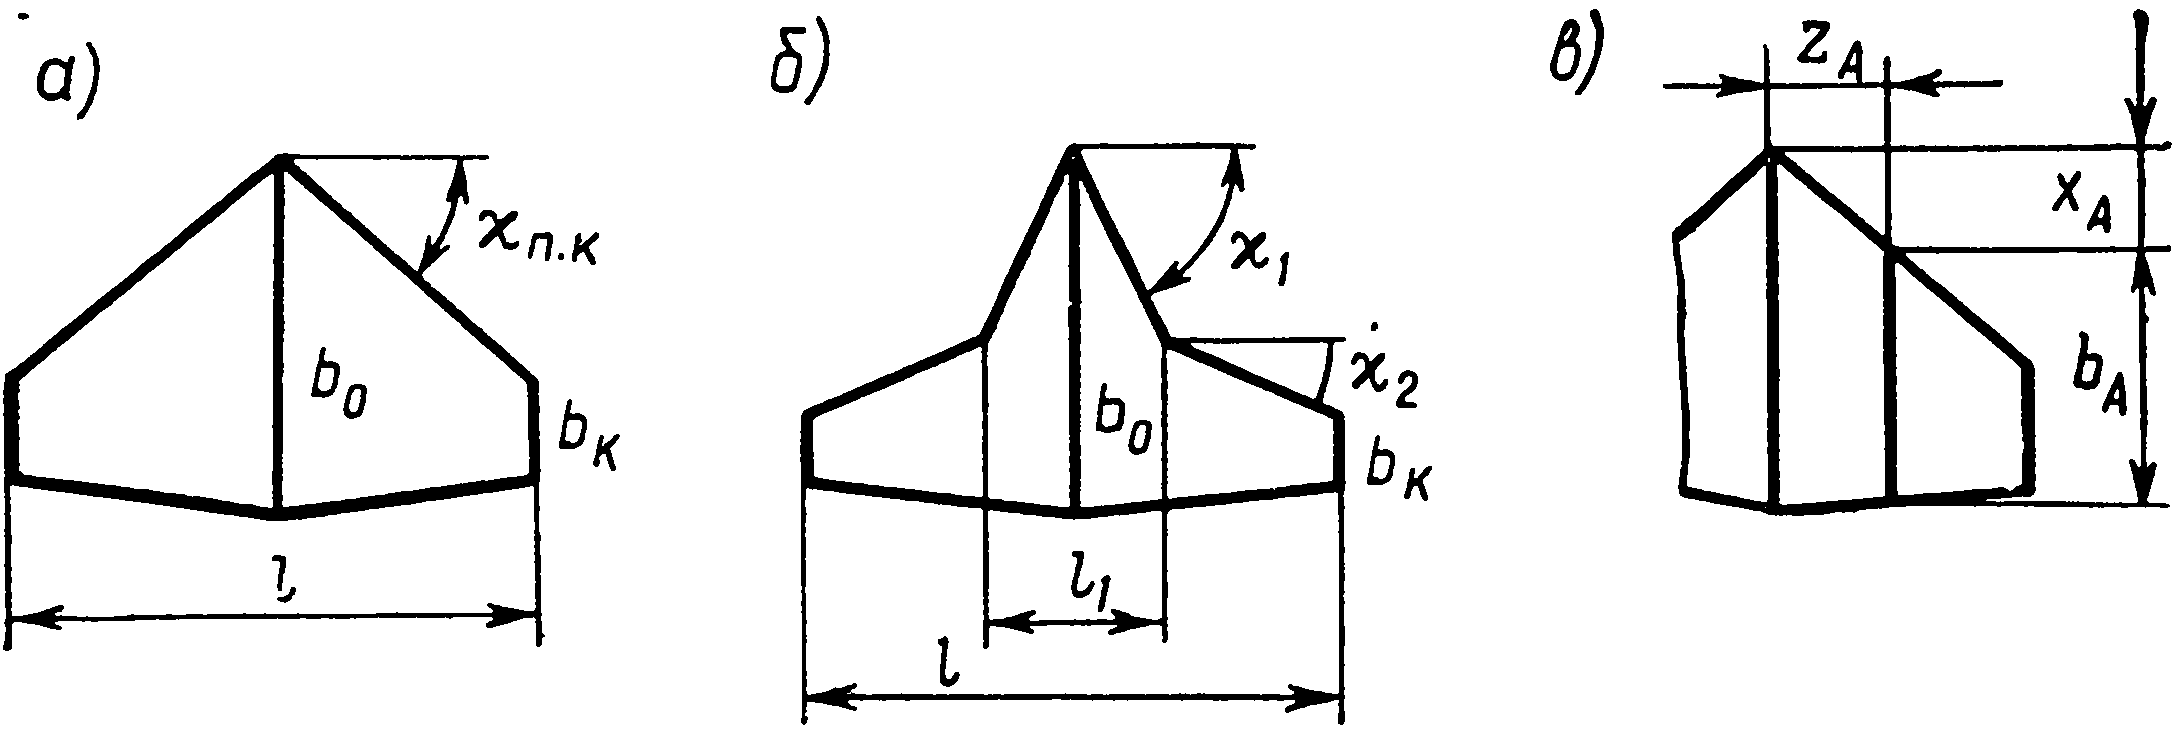
\includegraphics[width=0.7\linewidth]{img/wings-and-sach-ba}
		\caption{Стреловидное крыло \textit{(а)} и крыло сложной формы в плане \textit{(б)}, средняя аэродинамическая хорда $b_\mathrm{A}$ \textit{(в)}.}
		\label{fig:7.15_wings-and-sach-ba}
	\end{figure}
	Аэродинамические характеристики крыла конечного размаха зависят как от формы сечения, т. е. профиля, так и от формы крыла в плане. Форма крыла, показанная на \cref{fig:7.15_wings-and-sach-ba}, $a$, характеризуется углом стреловидности передней кромки $\chi_\mathrm{п.к}$ и двумя безразмерными параметрами --- удлинением $\lambda = l/b_\mathrm{ср}$, но $b_\mathrm{ср} = S/l$ и $\lambda = l^2/S$, сужением $\eta=b_0/b_\mathrm{к}$, где $l$ --- размах крыла, $S$ --- площадь крыла в плане, $b_0$, $b_\mathrm{к}$ --- корневая и концевые хорды крыла.\n
	На \cref{fig:7.15_wings-and-sach-ba} приведено крыло с прямой стреловидностью: $\chi_\mathrm{п.к}>0$. Для крыльев обратной стреловидности $\chi_\mathrm{п.к}<0$. В частных случаях, например для прямоугольного крыла, $\chi=0$, $\eta=1$, поэтому достаточно ввести один параметр --- $\lambda=l/b$; для треугольного крыла $n=\infty$, a $\lambda\tg\chi_\mathrm{п.к}=4$, т. е. также достаточно задать один параметр: $\lambda$ или $\chi_\mathrm{п.к}$.\n
	Для крыльев сложной формы в плане требуется задать более трех параметров. Например, для крыла, показанного на \cref{fig:7.15_wings-and-sach-ba}, \textit{б}, кроме удлинения и сужения необходимо ввести два угла стреловидности $\chi_1$ и $\chi_2$, а также относительную координату точки излома передней кромки $\bar{z}_1=l_1/l$.\n
	В качестве характерного линейного размера крыла обычно рассматривают среднюю хорду $b_\mathrm{ср}=S/l$ либо среднюю аэродинамическую хорду (СAX). Под средней аэродинамической хордой понимают хорду равновеликого прямоугольного крыла, имеющего те же аэродинамические характеристики $M_z$, $Y$, $X$, что и у исходного крыла.\n
	Из равенства моментов $M_z$ для заданного и прямоугольного крыльев, принимая, что коэффициенты момента и нормальной силы сечений вдоль размаха крыльев не изменяются, найдем среднюю аэродинамическую хорду $b_\mathrm{A}$ и координату $x_\mathrm{A}$ передней кромки САX (\cref{fig:7.15_wings-and-sach-ba}, \textit{в}):
	\begin{gather*}
		b_\mathrm{A} = \frac{2}{S}\int\limits_0^{\frac{l}{2}}b^2\dd z,\quad
		x_\mathrm{A} = \frac{2}{S}\int\limits_0^{\frac{l}{2}}bx\dd z.
	\end{gather*}\n
	Здесь $b$ --- хорда сечения крыла; $x$ --- координата передней кромки сечений крыла.\n
	Форма сечений крыла по его размаху может изменяться. Тогда имеют в виду аэродинамическую крутку. Крыло может иметь также геометрическую крутку, образованную переменным по размаху углом между хордой данного сечения и плоскостью $xz$.\n
	Рассмотрим некоторые особенности обтекания крыла конечного размаха. Как известно (см. \cref{sec:incompressible-flow-thin-profile}), аэродинамические характеристики сечений крыла бесконечного размаха одинаковы. Если же крыло имеет конечный размах, то в основном из-за перетекания воздуха через кромки с нижней поверхности на верхнюю (при положительном угле атаки) характеристики его сечений различны. При этом концы крыла оказывают существенное влияние на распределение скорости и давления по всей поверхности, особенно вблизи боковых кромок. Чем ближе к концам крыла, тем циркуляция скорости становится меньше: $\Gamma=\Gamma\left(z\right)$.\n
	Поскольку циркуляция скорости в сечении по теореме Стокса равна суммарной интенсивности вихрей, проходящих внутри контура, охватывающего сечение крыла, то интенсивность присоединенных вихрей, заменяющих крыло конечного размаха, изменяется не только по хорде, но и по размаху $\gamma\left(x,\; z\right)$. С другой стороны, на основании теоремы Гельмгольца интенсивность вихрей по длине вихревой трубки не изменяется. Поэтому уменьшение интенсивности присоединенного вихря вдоль размаха крыла возможно только в том случае, если с задней и боковых кромок крыла сходят вихри интенсивностью, соответствующей изменению циркуляции скорости по размаху $\left(-\dd\Gamma\right)$. Эти вихри называются \textit{свободными} и образуют за крылом вихревую пелену.\n
	\begin{figure}[htbp]
		\centering
		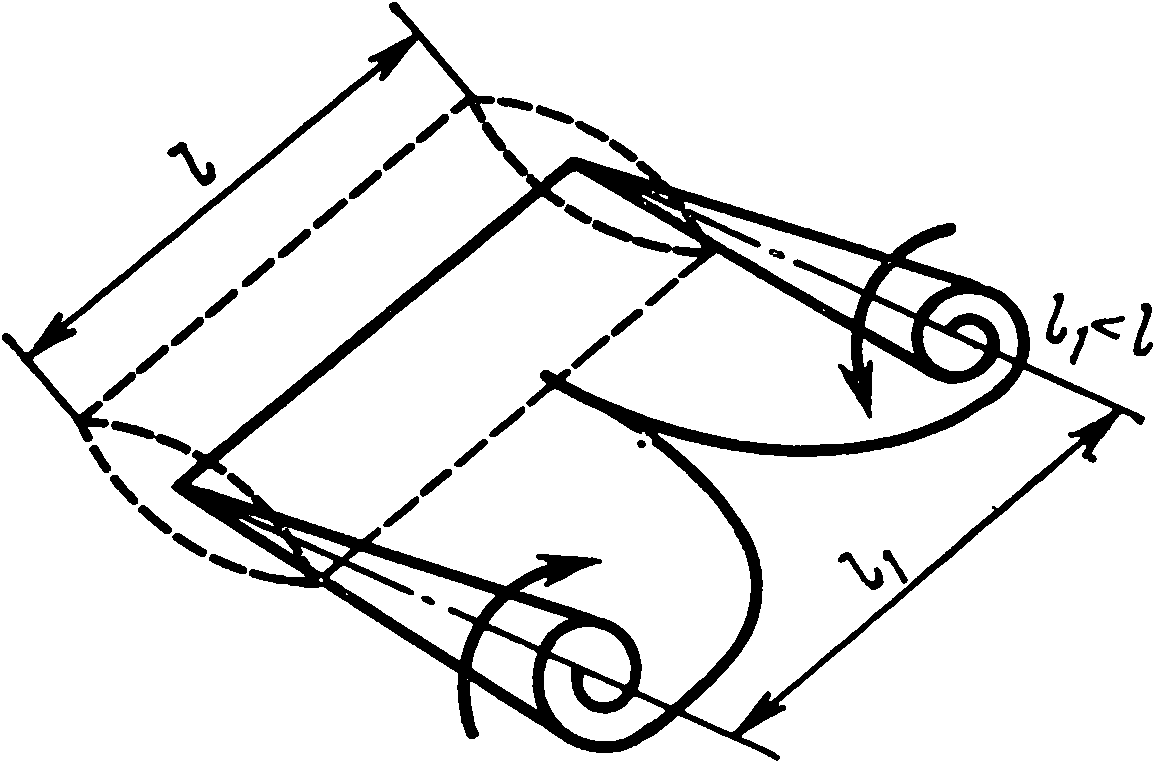
\includegraphics[width=0.3\linewidth]{img/vortex-sheet-folding}
		\caption{Свертывание вихревой пелены за крылом.}
		\label{fig:7.16_vortex-sheet-folding}
	\end{figure}
	Исследования вихревой пелены показывают, что она неустойчива и на некотором расстоянии от задней кромки сворачивается в два вихревых шнура (\cref{fig:7.16_vortex-sheet-folding}). При теоретических исследованиях крыло конечного размаха заменяется эквивалентной вихревой системой, состоящей из присоединенных вихрей $\gamma\left(x\; z\right)$, образующих несущую поверхность, и вихревой пелены, сходящей с задней и боковых кромок крыла, при малых углах атаки --- параллельно скорости невозмущенного потока. Подобная вихревая система положена в основу теории несущей поверхности.\n
	\begin{figure}[htbp]
		\centering
		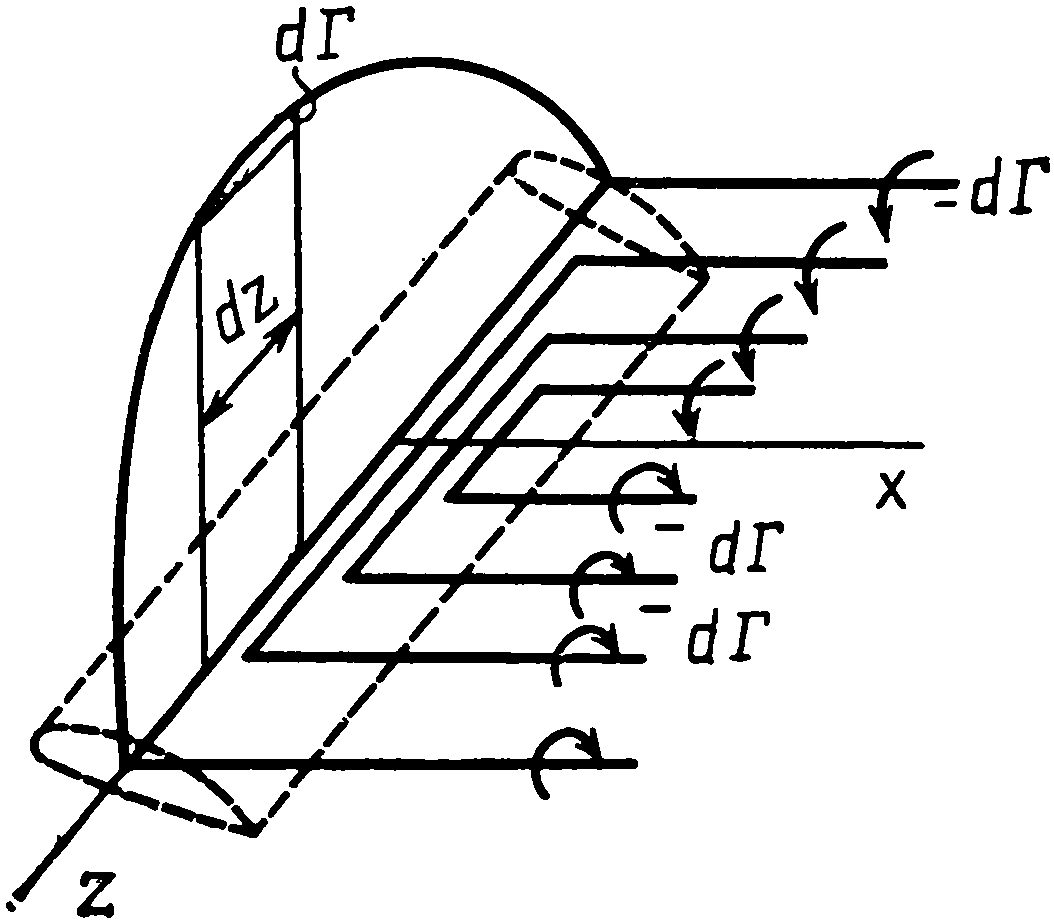
\includegraphics[width=0.3\linewidth]{img/U-shaped-vortices}
		\caption{Вихревая система крыла в виде совокупности П-образных вихрей.}
		\label{fig:7.17_u-shaped-vortices}
	\end{figure}
	В случае крыла достаточно большого удлинения $\left(\lambda>3\right)$, пренебрегая изменениям интенсивности присоединенных вихрей по хорде, вихревую поверхность приближенно можно заменить одним присоединенным вихрем (несущей линией) с интенсивностью $\Gamma\left(z\right)=\int_{0}^{b}\gamma\left(x,\;z\right)\dd x$. Этот вихрь обычно располагают вдоль линии центров давления. Тогда приближенно крыло можно заменить вихревой системой, состоящей из одного присоединенного вихря и вихревой пелены. Такая вихревая система используется в теории несущей линии. Вихревую систему крыла представим также в виде совокупности П-образных вихрей (\cref{fig:7.17_u-shaped-vortices}). П-образный вихрь состоит из отрезка присоединенного вихря и двух полубесконечных вихрей, сходящих с концов присоединенного вихря.\n
	Интенсивность каждого такого П-образного вихря постоянна и изменяется при переходе от одного вихря к другому.
	
	\subsection{Основы теории несущей линии. Понятия о скосе потока и индуктивном сопротивлении крыла}
	Рассмотрим обтекание крыла под некоторым углом атаки потоком со скоростью $v_\infty$. В соответствии с теорией несущей линии заменим крыло одним присоединенным вихрем и вихревой пеленой (\cref{fig:7.17_u-shaped-vortices}). На \cref{fig:7.17_u-shaped-vortices} ось $x$ направлена вдоль скорости невозмущенного потока $\vv{v}_\infty$. При этом в окрестности и, в частности, на поверхности крыла скорость $\vv{v}=\vv{v}_\infty+\vv{v}_i$, где $\vv{v}_i$ --- скорость, индуцированная вихрями в рассматриваемой точке. Так же как в теории тонкого профиля, на поверхности крыла примем $\vv{v}_i$ равной скорости в точках ее проекции на плоскость $xOz$. Эта скорость перпендикулярна плоскости $xOz$ (перпендикулярна направлению скорости невозмущенного потока), т. е. $\vv{v}_i=v_y$, и называется \textit{скоростью скоса потока}. Скорость $v_y$ изменяется как по размаху, так и по хорде крыла: $v_y\left(x,\;z\right)$. Однако для крыла достаточно большого удлинения, когда хорда мала по сравнению с размахом, изменением скорости $v_y$ по хорде в пределах одного и того же сечения можно пренебречь, считая ее постоянной и равной скорости скоса потока от свободных вихрей на оси присоединенного вихря. При этом $v_y$ изменяется по размаху: $v_y\left(z\right)$.\n
	\begin{figure}[htbp]
		\centering
		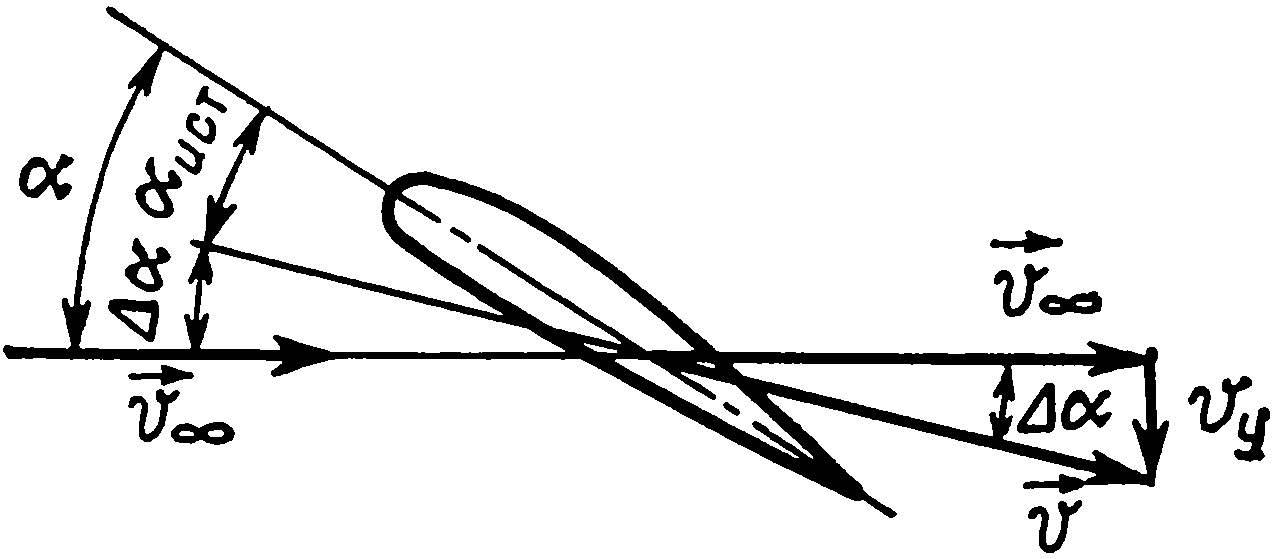
\includegraphics[width=0.35\linewidth]{img/flow-slope-and-true-alpha}
		\caption{Скос потока и истинный угол атаки.}
		\label{fig:7.18_flow-slope-and-true-alpha}
	\end{figure}
	Выясним, какие изменения в характер обтекания крыла вносит появление скорости $v_y$. Для этого рассмотрим произвольное сечение крыла (\cref{fig:7.18_flow-slope-and-true-alpha}). Наличие скорости $v_y$ здесь приводит к отклонению потока на угол $\Delta\alpha$, называемый \textit{углом скоса потока}.\n
	Так как угол $\Delta\alpha$ мал, то $\Delta\alpha\approx\tg\Delta\alpha=v_y/v_\infty$. В результате изменяется угол атаки сечений и крыла в целом. Истинный угол атаки $\alpha_\mathrm{ист}=\alpha-\Delta\alpha$.\n
	Воспользуемся теперь гипотезой плоских сечений, заключающейся в том, что при обтекании крыла каждое его сечение можно считать сечением крыла бесконечного размаха с соответствующим истинным углом атаки. Поэтому аэродинамические характеристики сечений крыла конечного размаха будем определять как характеристики профиля с учетом истинного угла атаки. Это основное положение теории несущей линии справедливо для крыльев достаточно большого удлинения $\left(\lambda>3\right)$ и при малых углах атаки.\n
	\begin{figure}[htbp]
		\centering
		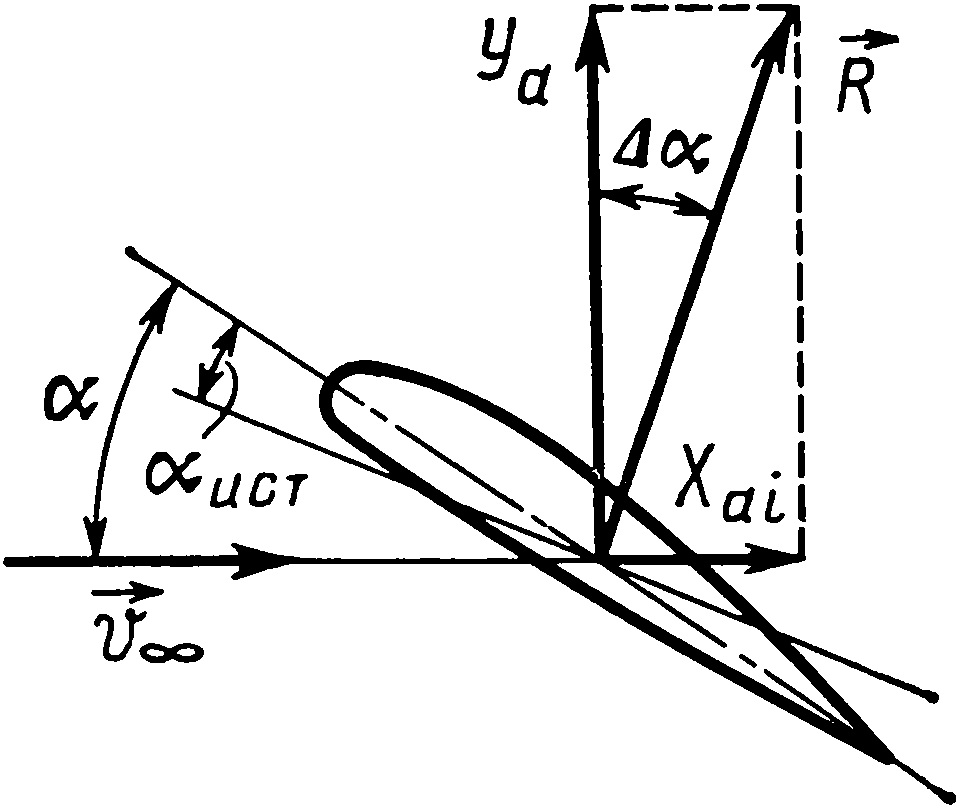
\includegraphics[width=0.3\linewidth]{img/wing-induced-drag}
		\caption{Индуктивное сопротивление крыла.}
		\label{fig:7.19_wing-induced-drag}
	\end{figure}
	Для крыла бесконечного размаха вектор результирующей силы согласно теореме Жуковского нормален к направлению невозмущенного потока. Тогда при наличии скоса потока вектор результирующей силы должен быть перпендикулярен направлению истинной скорости $\vv{v}$. Следовательно, скос потока приводит к отклонению результирующей силы от направления, перпендикулярного скорости невозмущенного потока, на угол $\Delta\alpha$ (\cref{fig:7.19_wing-induced-drag}). В результате появляется проекция силы вдоль направления невозмущенного потока. \underLine{Эта дополнительная сила $X_{\mathrm{a}i}\approx Y_\mathrm{a}\Delta\alpha$, которая возникает из-за скоса потока, называется индуктивным сопротивлением.} Если эту силу разделить на скоростной напор и площадь $\rho v_\infty^2 S/2$, то получим величину коэффициента индуктивного сопротивления:
	\begin{gather}\label{eq:757}
		c_{x\mathrm{a}i}=\frac{X_i}{\rho v_\infty^2 S/2}=c_{y\mathrm{a}}\Delta\alpha.
	\end{gather}\n
	Таким образом, сопротивление крыла конечного размаха состоит из профильного $c_{x\mathrm{a}p}$ и индуктивного сопротивлений, обусловленных скосом потока, т. е. для крыла конечного размаха $c_{x\mathrm{a}}=c_{x\mathrm{a}p}+c_{x\mathrm{a}i}$. У крыла бесконечного размаха, где скос потока отсутствует, индуктивное сопротивление равно нулю.\n
	\begin{figure}[htbp]
		\centering
		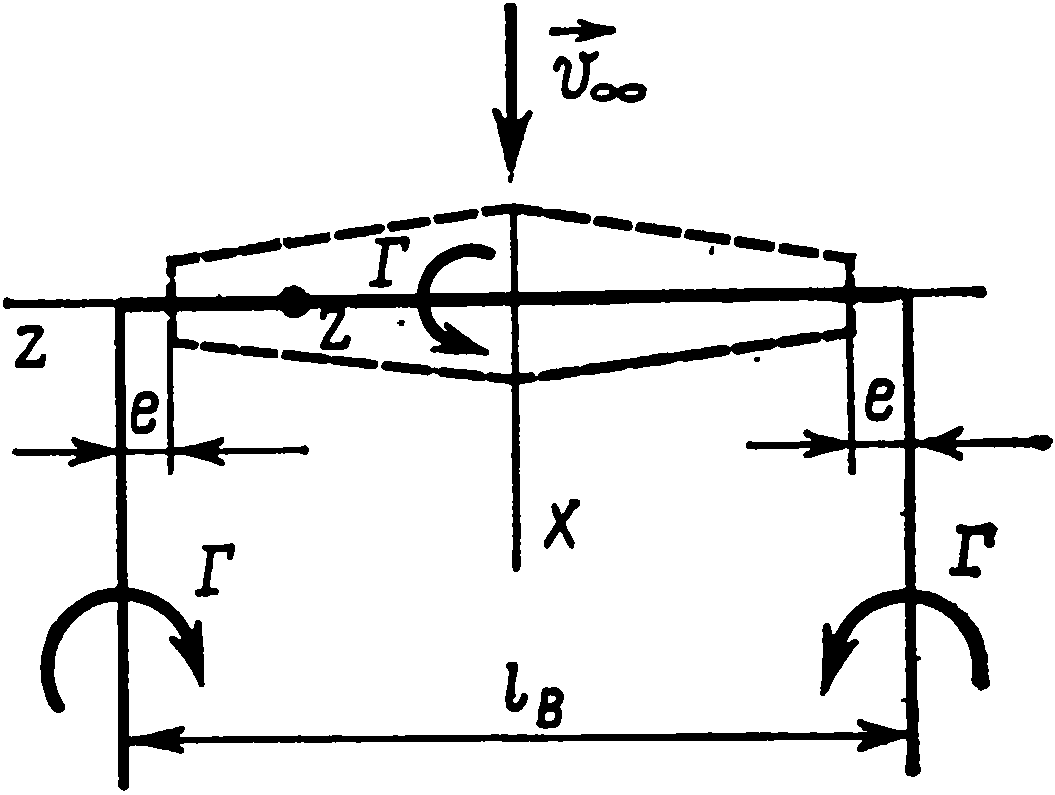
\includegraphics[width=0.3\linewidth]{img/vortex-system-approximate-determination-flow-slope-angle}
		\caption{Вихревая система крыла для приближенного определения среднего угла скоса потока.}
		\label{fig:7.20_vortex-system-approximate-determination-flow-slope-angle}
	\end{figure}
	Выведем приближенные соотношения, позволяющие оценить значения угла скоса потока, производной $c_{y\mathrm{a}}^\alpha$ и коэффициента $c_{x\mathrm{a}i}$ Для этого приближенно заменим крыло простейшей вихревой системой --- одним П-образным вихрем (\cref{fig:7.20_vortex-system-approximate-determination-flow-slope-angle}). Циркуляция скорости П-образного вихря при этом определяется из условия равенства подъемной силы крыла силе, создаваемой П-образным вихрем: $Y_\mathrm{a}=c_{y\mathrm{a}}\rho v_\infty^2 S/2 = \rho v_\infty\Gamma l_\mathrm{в}$, отсюда
	\begin{gather}\label{eq:758}
		\Gamma=\frac{\frac{1}{2}c_{y\mathrm{a}}Sv_\infty}{l_\mathrm{в}}.
	\end{gather}\n
	Расстояние между свободными вихрями при такой замене должно быть больше размаха крыла: $l_\mathrm{в}=l+2e$, где $e=\left(0,02\div0,04\right)l/2$.\n
	Скорость скоса потока $v_y\left(z\right)$ в произвольной точке несущей линии, вызываемая правым и левым полубесконечными свободными вихрями, определяется по формуле Био-Савара \eqref{eq:236}:
	\begin{gather}\label{eq:759}
		v_y\left(z\right)=\frac{\Gamma}{4\pi}\left(\frac{1}{\frac{l}{2}+e+z}+\frac{1}{\frac{l}{2}+l-z}\right),
	\end{gather}
	а средняя по размаху крыла скорость скоса потока
	\begin{gather*}
		v_y=\frac{1}{l}\int\limits_{-\frac{l}{2}}^{\frac{l}{2}}v_y\left(z\right)\dd z,
	\end{gather*}
	или, заменяя $v_y\left(z\right)$ выражением \eqref{eq:759}, имеем
	\begin{gather*}
		v_y=\frac{\Gamma}{2\pi l}\ln\frac{l+e}{e}.
	\end{gather*}\n
	Подставим в эту формулу выражение циркуляции скорости \eqref{eq:758}. Кроме того, учтем, что $l_\mathrm{в}=l\left(1+2e/l\right)$, а $l^2/S=\lambda$. При $e=0,04l/2$ ориентировочно принимаем $\frac{1}{1+2e/l}\ln\frac{l+e}{e}\approx 4$. Тогда
	\begin{gather}
		v_y=\frac{c_{y\mathrm{a}}v_\infty}{\pi\lambda};\label{eq:760}\\
		\Delta\alpha=\frac{c_{y\mathrm{a}}}{\pi\lambda}.\label{eq:761}
	\end{gather}\n
	Формулы \eqref{eq:760} и \eqref{eq:761} позволяют оценить значения скорости и угла скоса потока. Очевидно, что чем больше удлинение, тем меньше угол скоса потока. При $c_{y\mathrm{a}}$ угол $\Delta\alpha=0$, а с увеличением коэффициента подъемной силы угол скоса потока увеличивается.\n
	Используя выражение \eqref{eq:761}, выведем формулу для определения коэффициента подъемной силы. Для этого в формуле \eqref{eq:751} заменим геометрический угол атаки $\alpha$ истинным углом атаки $\alpha_\mathrm{ист}=\alpha-\Delta\alpha=\alpha-\frac{c_{y\mathrm{a}}}{\pi\lambda}$. Тогда $c_{y\mathrm{a}}=\frac{2\pi\left(\alpha-\alpha_0\right)}{1+2/\lambda}$. Дифференцируя по $\alpha$, имеем
	\begin{gather}\label{eq:762}
		c_{y\mathrm{a}}^\alpha=\frac{2\pi\lambda}{\lambda+2}.
	\end{gather}\n
	\begin{figure}[htbp]
		\centering
		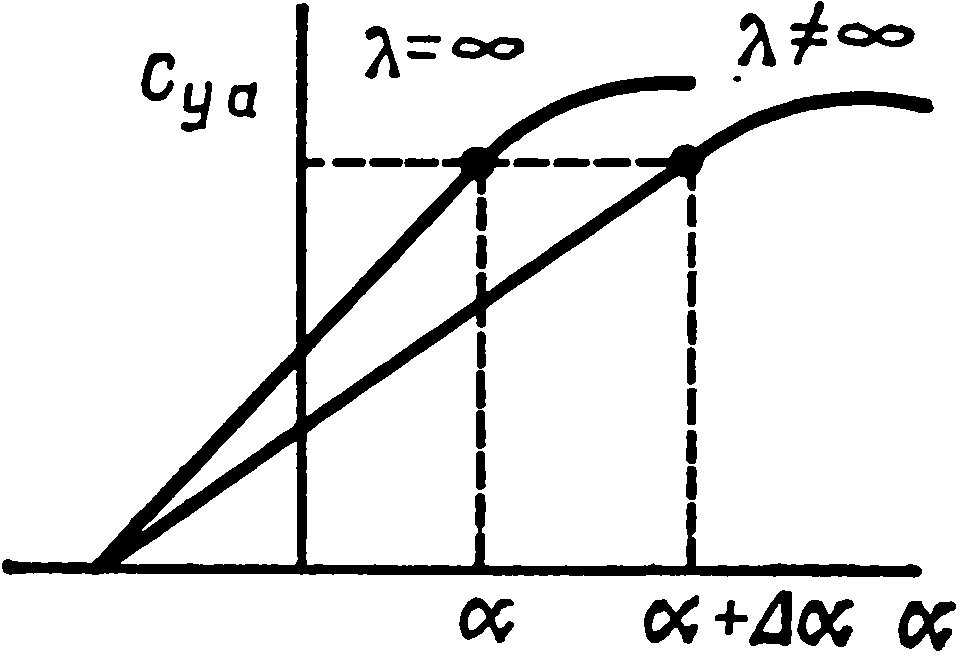
\includegraphics[width=0.3\linewidth]{img/Cya-vs-alpha}
		\caption{Коэффициенты подъемной силы крыла конечного и бесконечного размаха.}
		\label{fig:7.21_cya-vs-alpha}
	\end{figure}
	Отсюда следует, что с уменьшением удлинения коэффициент подъемной силы крыла уменьшается. Для получения одной и той же подъемной силы при прочих равных условиях крыло конечного размаха должно иметь больший угол атаки $\alpha+\Delta\alpha$, чем крыло бесконечного размаха (\cref{fig:7.21_cya-vs-alpha}).\n
	Выведем также выражение для определения коэффициента индуктивного сопротивления. Для этого подставим выражение \eqref{eq:761} в формулу \eqref{eq:757}:
	\begin{gather}\label{eq:763}
		c_{x\mathrm{a}i}=\frac{c_{y\mathrm{a}}^2}{\pi\lambda}.
	\end{gather}\n
	\begin{figure}[htbp]
		\centering
		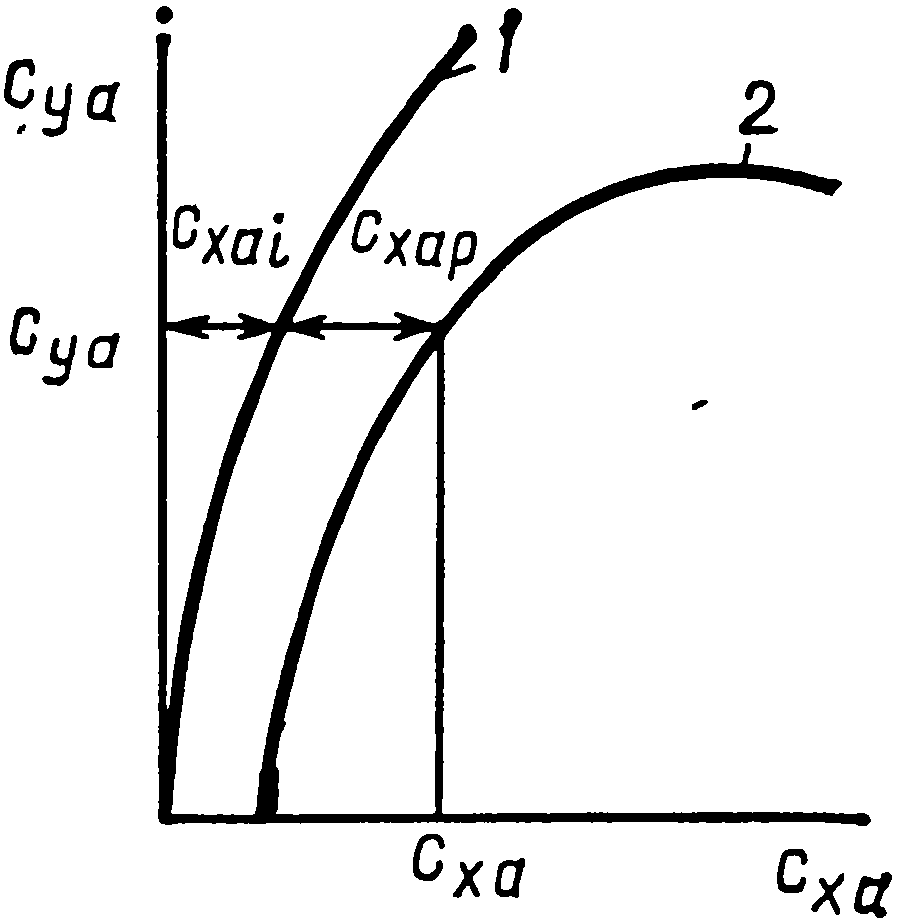
\includegraphics[width=0.25\linewidth]{img/induced-drag-parabola-and-wing-polar}
		\caption{Парабола индуктивного сопротивления \textit{1} и поляра крыла \textit{2}.}
		\label{fig:7.22_induced-drag-parabola-and-wing-polar}
	\end{figure}
	Таким образом, значение коэффициента индуктивного сопротивления тем меньше, чем больше удлинение крыла. В зависимости от $c_{y\mathrm{a}}$ коэффициент $c_{x\mathrm{a}i}$ изменяется по параболическому закону. Кривая $c_{x\mathrm{a}i}=f\left(c_{y\mathrm{a}}\right)$ называется \textit{параболой индуктивного сопротивления}, а кривая полного коэффициента сопротивления крыла в зависимости от коэффициента подъемной силы $c_{x\mathrm{a}}=F\left(c_{y\mathrm{a}}\right)$ --- \textit{полярой крыла} (\cref{fig:7.22_induced-drag-parabola-and-wing-polar}).\n
	Следует иметь в виду, что формулы \eqref{eq:762} и \eqref{eq:763} являются приближенными и не учитывают влияния формы крыла в плане. Однако основные зависимости коэффициентов $c_{y\mathrm{a}}$ от $\lambda$, a $c_{x\mathrm{a}i}$ от $c_{y\mathrm{a}}$ и $\lambda$ представлены в них точно. Более того, как показано ниже, формулы \eqref{eq:761} и \eqref{eq:763} совпадают с соответствующими формулами, полученными по теории несущей линии для крыльев с эллиптическим законом распределения циркуляции по размаху. В этом случае угол скоса потока постоянен вдоль размаха и определяется по формуле \eqref{eq:761}, а индуктивное сопротивление имеет минимальное значение по сравнению с любой другой формой крыла в плане и вычисляется по формуле \eqref{eq:763}.\n
	Применительно к крыльям произвольной формы в плане для определения производной $c_{y\mathrm{a}}^\alpha$ вместо формулы \eqref{eq:762} можно пользоваться следующим приближенным соотношением:
	\begin{gather}\label{eq:764}
		c_{y\mathrm{a}}^\alpha=\frac{2\pi\lambda}{P\lambda+2},
	\end{gather}
	где $P$ --- поправка, учитывающая влияние формы крыла в плане и представляющая собой отношение полупериметра крыла к его размаху.\n
	Для крыльев с прямой нестреловидной задней кромкой
	\begin{gather}\label{eq:765}
		P=\frac{1}{2}\left[1+\frac{1}{\lambda}\frac{4}{\eta+1}+\sqrt{1+\left(\frac{4}{\lambda}\right)^2\left(\frac{\eta-1}{\eta+1}\right)^2}\right].
	\end{gather}\n
	При $\lambda\to 0$ по формуле \eqref{eq:764} можно получить предельное значение производной $c_{y\mathrm{a}}^\alpha$ для крыльев достаточно малого удлинения: $\lambda\ll 1$.\n
	Из выражения \eqref{eq:765} следует, что для треугольного крыла $\left(\eta=\infty\right)$ при $\lambda\to 0$ значение $P\lambda\to 2$. Тогда
	\begin{gather}\label{eq:766}
		c_{y\mathrm{a}}^\alpha=\frac{\pi\lambda}{2}.
	\end{gather}
	Эта формула совпадает с формулой, полученной по теории тонкого тела, и дает удовлетворительные результаты при $\lambda<1$.\n
	Отметим, что формулы \eqref{eq:762} -- \eqref{eq:764} являются приближенными. Поэтому ими можно пользоваться только для расчетов с целью приближенной оценки величин $c_{y\mathrm{a}}^\alpha$ и $c_{x\mathrm{a}i}$.
	
	\newpage
	\part{Пограничный слой и аэродинамический нагрев при больших скоростях}\label{prt:boundary-layer}
	
	\section{Лекция 6}
	
	\subsection{Понятие о пограничном слое}
	\begin{figure}[htbp]
		\centering
		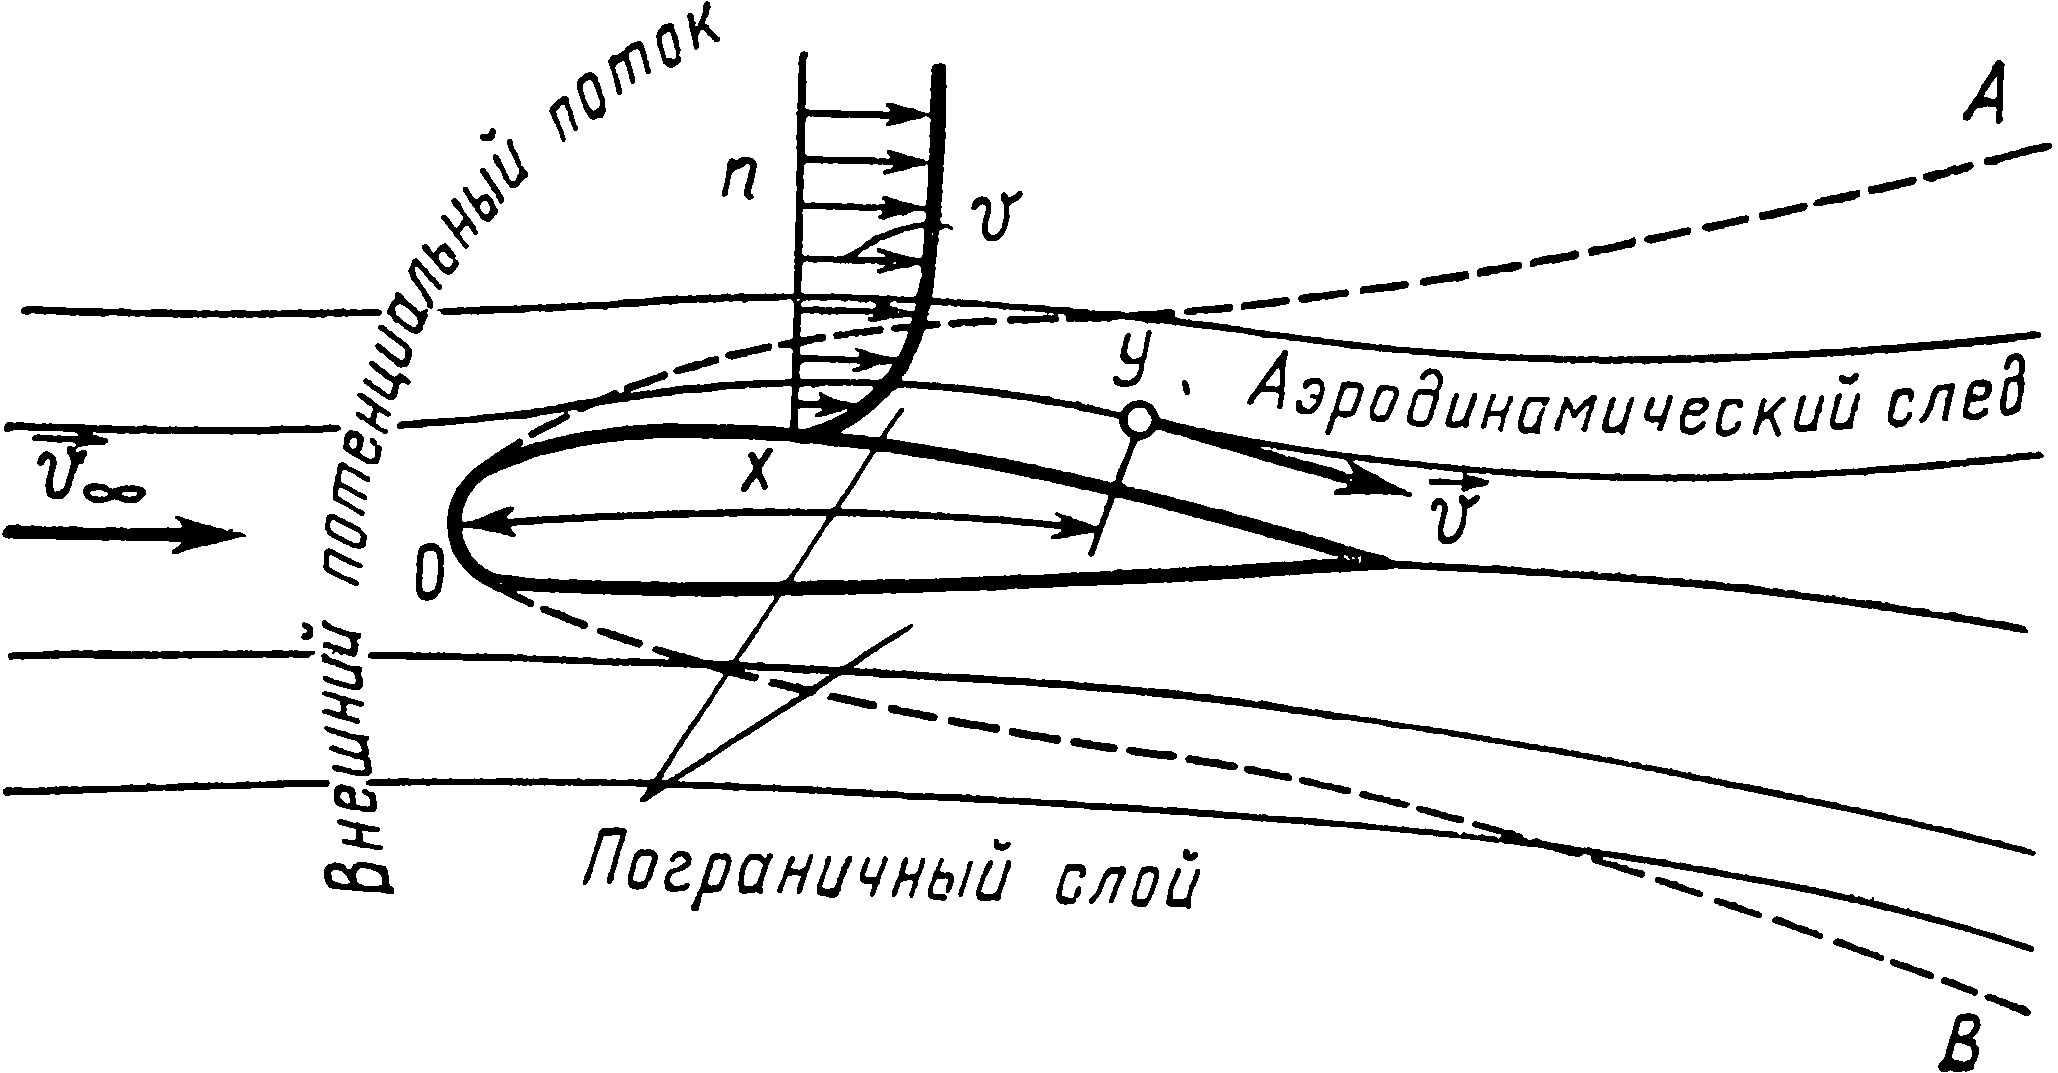
\includegraphics[width=0.7\linewidth]{img/boundary-layer}
		\caption{Пограничный слой.}
		\label{fig:12.1_boundary-layer}
	\end{figure}
	Рассмотрим физическую сущность обтекания. Допустим, что неподвижное тело обтекается потоком вязкого газа (\cref{fig:12.1_boundary-layer}). Непосредственные наблюдения показывают, что в тонком слое вблизи поверхности тела скорость потока резко нарастает --- от значения $v = 0$ (на поверхности тела) до величины порядка скорости набегающего потока. \underLine{Тонкий слой газа, прилегающий к поверхности обтекаемого тела и представляющий собой область больших значений градиентов скорости по нормали к телу, называют \textit{пограничным слоем}.}\n
	Частицы газа в пограничном слое, пройдя вдоль поверхности обтекаемого тела, уносятся потоком. Скорости этих частиц, как правило, меньше скорости в окружающей среде. Заторможенные частицы образуют за телом область, называемую \textit{аэродинамическим следом}.\n
	Формула Ньютона для силы внутреннего трения $\tau = \mu\frac{\pp v}{\pp n}$ показывает, что \underLine{внутри пограничного слоя и следа, где градиенты скорости значительны, силой внутреннего трения пренебрегать нельзя и среду в пограничном слое следует считать вязкой даже при малом значении коэффициента $\mu$. Вне пограничного слоя и следа за телом, где градиенты скорости малы, силой внутреннего трения можно пренебречь, т. е. считать среду невязкой.}\n
	Таким образом, движение среды вне пограничного слоя и следа можно изучать с помощью уравнений Эйлера. Внутри пограничного слоя среду следует рассматривать как вязкую и изучать ее движение с помощью уравнений движения вязкой среды.\n
	Введем понятие о толщине пограничного слоя. На поверхности скорость потока $v = 0$, а при удалении от поверхности эта скорость асимптотически приближается к скорости в невязком потоке, причем уже на достаточно малом расстоянии от поверхности она незначительно отличается от нее. Толщина пограничного слоя --- величина условная. Обычно за толщину пограничного слоя $\delta$ в данной точке поверхности принимают расстояние от тела до такой точки, в которой действительная скорость потока отличается от скорости в невязком потоке на 1\%. Толщина пограничного слоя зависит от положения точки на поверхности. На передней кромке толщина $\delta = 0$ и увеличивается при удалении от нее.\n
	
	\subsection{Дифференциальные уравнения пограничного слоя в несжимаемой среде}
	\begin{figure}[htbp]
		\centering
		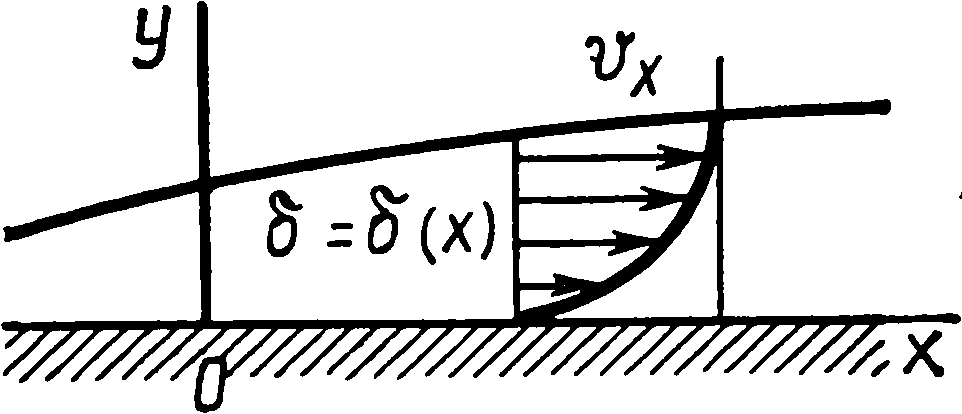
\includegraphics[width=0.35\linewidth]{img/differential-equations-boundary-layer-scheme}
		\caption{Схема к выводу дифференциальных уравнений пограничного слоя.}
		\label{fig:12.5_differential-equations-boundary-layer-scheme}
	\end{figure}
	Выведем сначала дифференциальные уравнения для плоского пограничного слоя в установившемся потоке несжимаемой среды (\cref{fig:12.5_differential-equations-boundary-layer-scheme}).\n
	Для изучения установившегося движения в пограничном слое используем дифференциальные уравнения \eqref{eq:323}, которые в рассматриваемом случае имеют следующий вид:
	\begin{gather*}
		v_x\frac{\pp v_x}{\pp x} + v_y\frac{\pp v_x}{\pp y} = X - \frac{1}{\rho}\frac{\pp p}{\pp x} + \nu\left(\frac{\pp^2 v_x}{\pp x^2} + \frac{\pp^2 v_x}{\pp y^2}\right);\\
		v_x\frac{\pp v_y}{\pp x} + v_y\frac{\pp v_y}{\pp y} = Y - \frac{1}{\rho}\frac{\pp p}{\pp y} + \nu\left(\frac{\pp^2 v_y}{\pp x^2} + \frac{\pp^2 v_y}{\pp y^2}\right).
	\end{gather*}\n
	Пренебрегая массовыми силами $X$ и $Y$ и присоединяя к уравнениям движения уравнение неразрывности, получаем следующую систему дифференциальных уравнений:
	\begin{gather}\label{eq:1211}
		\begin{gathered}
			v_x\frac{\pp v_x}{\pp x} + v_y\frac{\pp v_x}{\pp y} = -\frac{1}{\rho}\frac{\pp p}{\pp x} + \nu\left(\frac{\pp^2 v_x}{\pp x^2} + \frac{\pp^2 v_x}{\pp y^2}\right);\\
			v_x\frac{\pp v_y}{\pp x} + v_y\frac{\pp v_y}{\pp y} = -\frac{1}{\rho}\frac{\pp p}{\pp y} + \nu\left(\frac{\pp^2 v_y}{\pp x^2} + \frac{\pp^2 v_y}{\pp y^2}\right);\\
			\frac{\pp v_x}{\pp x} + \frac{\pp v_y}{\pp y} = 0.
		\end{gathered}
	\end{gather}\n
	Величина входящей в эти уравнения координаты $y$ в пограничном слое ограничена неравенством $0 \leqslant y \leqslant \delta\left(x\right)$. Это означает, что в уравнениях координату $y$ можно считать малой величиной порядка $\delta$. Заметим, что малость $\delta$ следует понимать в том смысле, что мало отношение $\delta/l$, где $l$ --- характерный размер обтекаемого тела (например, его длина). Имея это в виду, оценим порядок членов, входящих в уравнения \eqref{eq:1211}.\n
	Так как на стенке обтекаемого тела $v_x = 0$, а на внешней границе слоя $v_x$ имеет порядок $v$, где $v$ --- характерная скорость рассматриваемого течения (например, скорость на бесконечности перед телом), то отсюда следует, что при изменении координаты $y$ от 0 до $\delta$ приращение $\Delta v_x$ имеет порядок $v$, а приращение $\Delta y$ --- порядок $\delta$. Поэтому $\frac{\pp v_x}{\pp y} \sim \frac{v}{\delta}$. Аналогично можно показать, что внутри пограничного слоя $\frac{\pp^2 v_x}{\pp y^2} \sim \frac{v}{\delta^2}$. Чтобы оценить порядок $\frac{\pp v_x}{\pp x}$, заметим, что при перемещении вдоль обтекаемого контура на отрезок порядка характерной длины $l$ скорость $v_x$ может измениться на величину порядка $v$ (например, от $0$ до $v$), т. е. и в этом случае $\Delta v_x \sim v$. Так как при этом $\Delta x \sim l$, то $\frac{\pp v_x}{\pp x} \sim \frac{v}{l}$.\n
	Нетрудно убедиться, что $\frac{\pp^2 v_x}{\pp x^2} \sim \frac{v}{l^2}$. Используя затем уравнение неразрывности $\frac{\pp v_x}{\pp x} = -\frac{\pp v_y}{\pp y}$, делаем вывод, что $\frac{\pp v_y}{\pp y}$ имеет тот же порядок, что и $\frac{\pp v_x}{\pp x}$, т. е. $\frac{\pp v_y}{\pp y} \sim \frac{v}{l}$.\n
	Поскольку $v_y = \int_{0}^{y}\frac{\pp v_y}{\pp y}\dd y$, то $v_y \sim v\frac{\delta}{l}$.\n
	Имея в виду, что на поверхности обтекаемого тела $v_y = 0$, и используя полученную оценку порядка величины $v_y$ в точках внутри слоя, найдем порядок величины производных $\frac{\pp v_y}{\pp x}$, $\frac{\pp^2 v_y}{\pp x^2}$, $\frac{\pp^2 v_y}{\pp y^2}$: $\frac{\pp v_y}{\pp x} \sim v\frac{\delta}{l^2}$, $\frac{\pp^2 v_y}{\pp x^2} \sim v\frac{\delta}{l^2}$, $\frac{\pp^2 v_y}{\pp y^2} \sim \frac{v}{l\delta}$.\n
	Определив порядок скоростей и их производных, входящих в уравнения \eqref{eq:1211}, представим первое из этих уравнений, подставив под каждым членом порядок его величин:
	\begin{gather*}
		v_x\underbrace{\frac{\pp v_x}{\pp x}}_{\dfrac{v^2}{l}} + v_y\underbrace{\frac{\pp v_x}{\pp y}}_{\dfrac{v^2}{l}} = -\frac{1}{\rho}\frac{\pp p}{\pp x} + \nu\biggl(\underbrace{\frac{\pp^2 v_x}{\pp x^2}}_{\dfrac{v}{l^2}} + \underbrace{\frac{\pp^2 v_x}{\pp y^2}}_{\dfrac{v}{\delta^2}}\biggr).
	\end{gather*}\n
	В этом уравнении можно отбросить член $\frac{\pp^2 v_x}{\pp x^2}$, как малый по сравнению с членом $\frac{\pp^2 v_x}{\pp y^2}$. Тогда первое уравнение системы \eqref{eq:1211} примет вид
	\begin{gather*}
		v_x\frac{\pp v_x}{\pp x} + v_y\frac{\pp v_x}{\pp y} = -\frac{1}{\rho}\frac{\pp p}{\pp x} + \nu\frac{\pp^2 v_x}{\pp y^2}.
	\end{gather*}\n
	Внутри пограничного слоя инерционные и вязкие силы имеют одинаковый порядок. Тогда отношение $\frac{v^2/l}{\nu v/\delta^2} = \left(\frac{\delta}{l}\right)^2\Rey$ должно иметь порядок, равный единице, т. е. $\left(\frac{\delta}{l}\right)^2\Rey \approx 1$. Отсюда следует, что отношение $\frac{\delta}{l} \sim \frac{1}{\sqrt{\Rey}}$.\n
	Рассмотрим теперь второе уравнение \eqref{eq:1211}:
	\begin{gather*}
		v_x\underbrace{\frac{\pp v_y}{\pp x}}_{\dfrac{v^2\delta}{l^2}} + v_y\underbrace{\frac{\pp v_y}{\pp y}}_{\dfrac{v^2\delta}{l^2}} = -\frac{1}{\rho}\frac{\pp p}{\pp y} + \nu\Biggl(\underbrace{\frac{\pp^2 v_y}{\pp x^2}}_{\dfrac{v\delta}{l^2}} + \underbrace{\frac{\pp^2 v_y}{\pp y^2}}_{\dfrac{v}{l\delta}}\Biggr).
	\end{gather*}\n
	Пренебрегая членом $\frac{\pp^2 v_y}{\pp x^2}$, так как он мал по сравнению с $\frac{\pp^2 v_y}{\pp y^2}$, представим это уравнение в виде
	\begin{gather}\label{eq:1212}
		v_x\frac{\pp v_y}{\pp x} + v_y\frac{\pp v_y}{\pp y} = -\frac{1}{\rho}\frac{\pp p}{\pp y} + \nu\frac{\pp^2 v_y}{\pp y^2}.
	\end{gather}\n
	Инерционные и вязкие члены второго уравнения системы \eqref{eq:1211} имеют порядок $\frac{v^2\delta}{l^2}$ или $\frac{v^2}{l\sqrt{\Rey}}$.\n
	Тот же порядок, что и сохраняемые во втором уравнении члены, имеет и величина $\frac{1}{\rho}\frac{\pp p}{\pp y}$, т. е. производной $\frac{\pp p}{\pp y}$ можно пренебречь по сравнению с производной $\frac{\pp p}{\pp x}$, имеющей порядок $\frac{v^2}{l}$. Тогда второе уравнение системы \eqref{eq:1211} можно опустить, заменив его уравнением
	\begin{gather}\label{eq:1213}
		\frac{\pp p}{\pp y} = 0,
	\end{gather}
	которое означает, что \textit{давление внутри пограничного слоя не изменяется вдоль нормали к контуру тела и равно давлению на внешней границе слоя}.\n
	Из уравнения \eqref{eq:1213} следует также, что распределение давления вдоль поверхности совпадает с распределением давления по границе пограничного слоя. Этот результат подтверждается экспериментом. Давление на границе пограничного слоя можно найти, решая задачу обтекания тела потенциальным потоком.\n
	Для плоского установившегося движения, заменяя частную производную $\frac{\pp p}{\pp x}$ на полную $\frac{\dd p}{\dd x}$, так как в этом случае давление $p$ является функцией только координаты $x$, и используя уравнение неразрывности, получаем следующую систему дифференциальных уравнений пограничного слоя в несжимаемой среде (уравнение Прандтля):
	\begin{gather}\label{eq:1214}
		v_x\frac{\pp v_x}{\pp x} + v_y\frac{\pp v_x}{\pp y} = -\frac{1}{\rho}\frac{\dd p}{\dd x} + \nu\frac{\pp^2 v_x}{\pp y^2}, \quad \frac{\pp v_x}{\pp x} + \frac{\pp v_y}{\pp y} = 0.
	\end{gather}\n
	Система уравнений \eqref{eq:1214} интегрируется при следующих граничных условиях:
	\begin{gather*}
		v_x = v_y = 0 \hspace{0.5em} \mathrm{при} \hspace{0.5em} y = 0; \quad v_x = u\left(x\right) \hspace{0.5em} \mathrm{при} \hspace{0.5em} y = \infty.
	\end{gather*}
	Здесь $u\left(x\right)$ --- скорость на верхней границе пограничного слоя.\n
	Поскольку уравнения \eqref{eq:1214} для составляющей скорости $v_y$, являются уравнениями первого порядка, то для определения $v_y$ достаточно задать одно условие (на поверхности тела).\n
	Дифференциальные уравнения \eqref{eq:1214} для несжимаемого пограничного слоя получены в предположении, что граница твердого тела плоская. Эти уравнения с достаточной точностью справедливы и для криволинейной стенки. В этом случае следует отсчитывать абсциссу $x$ по дуге контура тела, а ординату $y$ --- по нормали к поверхности тела.
	
	\subsection{Интегральное соотношение пограничного слоя}
	\begin{figure}[htbp]
		\centering
		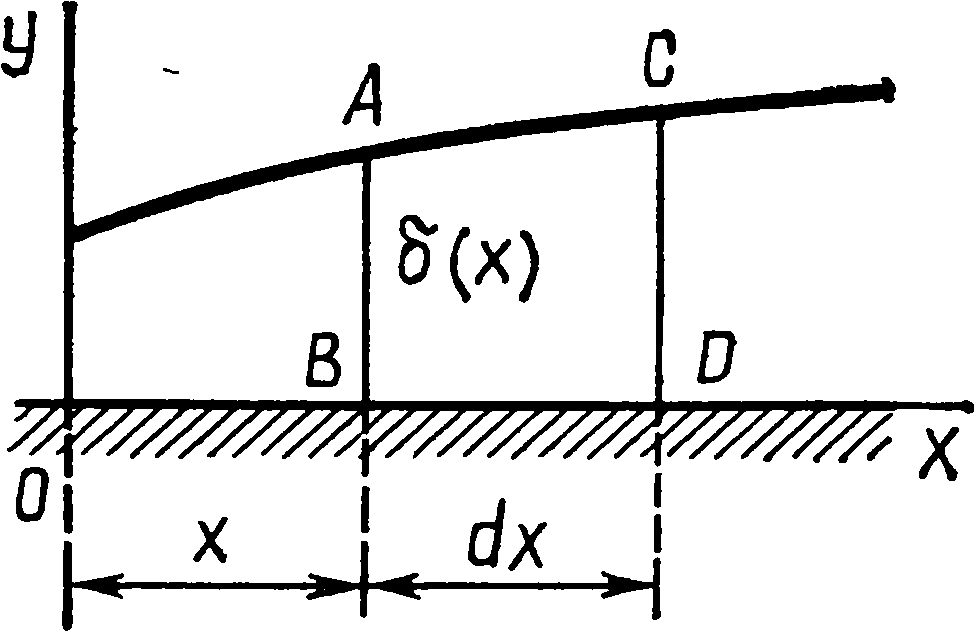
\includegraphics[width=0.35\linewidth]{img/integral-relation-boundary-layer-scheme}
		\caption{Схема к выводу интегрального соотношения пограничного слоя.}
		\label{fig:12.6_integral-relation-boundary-layer-scheme}
	\end{figure}
	Рассмотрим случай установившегося плоского пограничного слоя. Выделим в этом слое бесконечно малый объем $ABDC$ (\cref{fig:12.6_integral-relation-boundary-layer-scheme}), ограниченный элементом $BD$ твердой границы, которую примем за ось $x$, элементом $AC$ верхней границы пограничного слоя и плоскостями $AB$ и $CD$, отстоящими друг от друга на расстоянии $\dd x$. Протяженность объема в направлении оси $z$ примем равной единице. Применим к объему $ABDC$ теорему об изменении количества движения. Вычислим изменение количества движения в направлении оси $x$ за промежуток времени $\dd t$. Очевидно, через участок $AB$ втекает масса газа $\dd t\int_{0}^{\delta}\rho v_x\dd y$, а через участок $CD$ --- $\dd t\int_{0}^{\delta}\rho v_x\dd y + \dd t\left(\frac{\dd}{\dd x}\int_{0}^{\delta}\rho v_x \dd y\right)\dd x$.\n
	Разность между ними составляет $\dd t\left(\frac{\dd}{\dd x}\int_{0}^{\delta}\rho v_x\dd y\right)\dd x$.\n
	На основании условия неразрывности для установившегося течения через верхнюю границу $AC$ втекает такая же масса газа. Она вносит следующее количество движения: $u\dd t\dd x\frac{\dd}{\dd x}\int_{0}^{\delta}\rho v_x\dd y$. Здесь $u$ --- скорость потока на внешней границе пограничного слоя.\n
	Подсчитаем количества движения газа, вносимого и уносимого через участки $AB$ и $CD$. Через участок $AB$ вносится количество движения $\dd t\int_{0}^{\delta}\rho v_x^2\dd y$. Количество движения, уносимого газом через участок $CD$, будет $\dd t\int_{0}^{\delta}\rho v_x^2\dd y + \dd t\left(\frac{\dd}{\dd x}\int_{0}^{\delta}\rho v_x^2\dd y\right)\dd x$. Тогда разность количеств движения составляет $\dd t\left(\frac{\dd}{\dd x}\int_{0}^{\delta}\rho v_x^2\dd y\right)\dd x$.\n
	Найдем полное изменение количества движения газа в объеме за время $\dd t$:
	\begin{subequations}
		\begin{gather}\label{eq:12.4(a)}
			\left[\frac{\dd}{\dd x}\int\limits_0^\delta\rho v_x^2\dd y - u\frac{\dd}{\dd x}\int\limits_0^\delta\rho v_x\dd y\right]\dd x\dd t.
		\end{gather}\n
		Вычислим импульсы внешних сил за тот же промежуток времени $\dd t$ в направлении оси $x$. Очевидно, на элемент $ABCD$ в этом направлении действуют силы давления, приложенные к левой, верхней и правой граням элемента, и сила трения, приложенная к нижней его грани $BD$. Проекции на ось $x$ сил давления, действующих на грани $AB$, $AC$ и $DC$, соответственно равны $p\delta$, $p\dd\delta$, $-\left(p\delta + \frac{\dd\left(p\delta\right)}{\dd x}\dd x\right)$.\n
		Сумма проекций сил давления
		\begin{gather*}
			p\delta + p\dd\delta - \left(p\delta + \frac{\dd \left(p\delta\right)}{\dd x}\dd x\right) = -\delta\frac{\dd p}{\dd x}\dd x,
		\end{gather*}
		а импульс сил за время $\dd t$ составит
		\begin{gather}\label{eq:12.4(б)}
			-\delta\frac{\dd p}{\dd x}\dd t\dd x.
		\end{gather}\n
		Импульс силы трения, действующей на элементе поверхности $BD$,
		\begin{gather}\label{eq:12.4(в)}
			-\tau_0\dd x\dd t.
		\end{gather}\n
	\end{subequations}
	Приравнивая выражение \eqref{eq:12.4(a)} для изменения количества движения сумме величин \eqref{eq:12.4(б)} и \eqref{eq:12.4(в)} для импульсов действующих сил, получаем искомое интегральное соотношение пограничного слоя для случая плоского установившегося движения газа (\textit{интегральное соотношение Кармана}):
	\begin{gather}\label{eq:1222}
		\frac{\dd}{\dd x}\int\limits_0^\delta\rho v_x^2\dd y - u\frac{\dd}{\dd x}\int\limits_0^\delta\rho v_x\dd y = -\delta\frac{\dd p}{\dd x} - \tau_0.
	\end{gather}\n
	Следует отметить, что интегральное соотношение \eqref{eq:1222} пригодно для изучения не только ламинарного, но и турбулентного движения внутри пограничного слоя. Входящие в интегральное соотношение пограничного слоя величины $u$, $p$ можно рассматривать как известные, тогда для несжимаемой среды неизвестными будут только $v_x$, $\delta$ и $\tau_0$, а с учетом сжимаемости --- $v_x$, $\delta$, $\tau_0$, $\rho$.\n
	При использовании интегрального соотношения \eqref{eq:1222} нужны два дополнительных уравнения: закон распределения скорости по нормали к поверхности в пограничном слое, который в этом случае можно задать приближенно соответствующей аппроксимирующей функцией, а в качестве второго уравнения для определенного режима течения вязкой среды в пограничном слое --- закон напряжения трения. Например, для ламинарного пограничного слоя можно использовать формулу Ньютона $\tau_0 = \mu\left(\frac{\pp v_x}{\pp y}\right)_{y = 0}$.\n
	В результате подстановки выражений для $v_x$ и $\tau_0$ в интегральное соотношение получаем обыкновенное дифференциальное уравнение для определения толщины пограничного слоя.
	
	\subsection{Расчет пограничного слоя на плоской пластинке в несжимаемой среде}
	\begin{figure}[htbp]
		\centering
		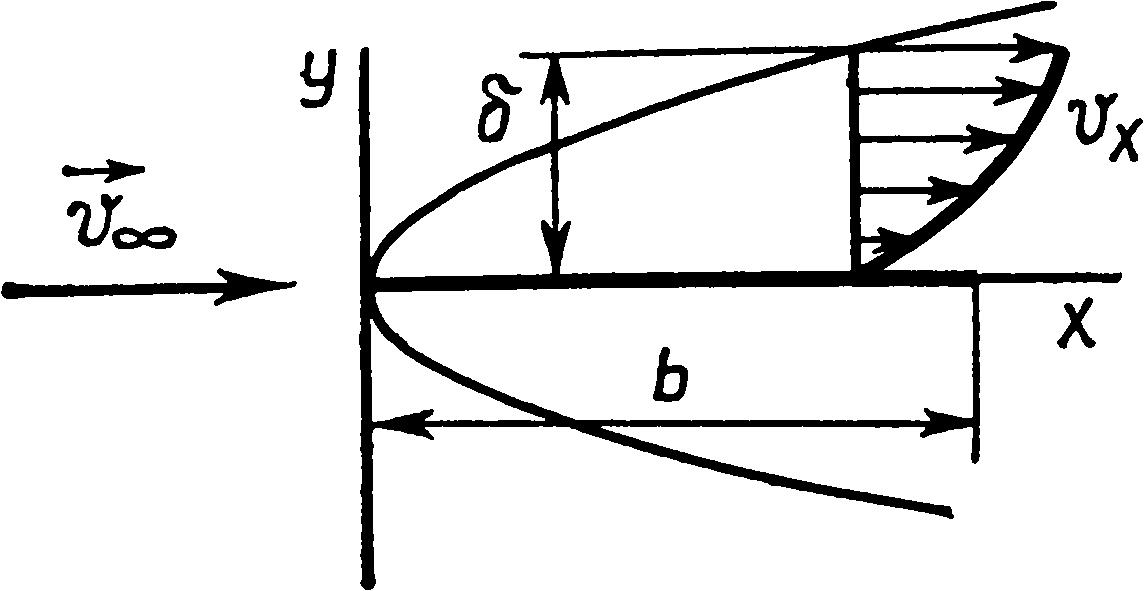
\includegraphics[width=0.3\linewidth]{img/flat-plate-boundary-layer}
		\caption{Пограничный слой на плоской пластинке.}
		\label{fig:12.7_flat-plate-boundary-layer}
	\end{figure}
	Решение задачи об обтекании плоской пластинки в теории сопротивления трения имеет большое значение. Пластинка (\cref{fig:12.7_flat-plate-boundary-layer}), поставленная вдоль потока, является простейшим удобообтекаемым телом, сопротивление которого зависит только от касательных напряжений. Найденные для пластинки зависимости коэффициента сопротивления трения можно использовать при приближенных расчетах сопротивления трения удобообтекаемых тел, например тонких профилей, крыльев и корпусов.\n
	Задача расчета пограничного слоя в несжимаемом потоке сводится к определению закона изменения толщины пограничного слоя, т. е. к функции $\delta = \delta\left(x\right)$, и силы сопротивления трения $X_\mathrm{тр}$ при условии, что известны скорость набегающего потока $v_\infty$ и кинематическая вязкость среды $\nu$.\n
	Для решения задачи воспользуемся интегральным соотношением пограничного слоя \eqref{eq:1222}. Так как в рассматриваемом случае $u = v_\infty$ и $\frac{\dd p}{\dd x} = 0$, т. е. пластинка представляет собой тело с нулевым градиентом давления вдоль по хорде, то интегральное соотношение \eqref{eq:1222} принимает вид
	\begin{gather}\label{eq:1223}
		\frac{\dd}{\dd x}\int\limits_0^\delta\rho v_x^2\dd y - v_\infty\frac{\dd}{\dd x}\int\limits_0^\delta\rho v_x\dd y = -\tau_0.
	\end{gather}\n
	Уравнением \eqref{eq:1223} можно пользоваться для расчета как ламинарного, так и турбулентного пограничного слоев на плоской пластинке.
	
	\subsubsection{Расчет ламинарного пограничного слоя}
	Зададим $v_x/v_\infty$ в виде полинома третьей степени относительно безразмерной координаты $y/\delta$, т. e. $v_x/v_\infty = a_0 + a_1y/\delta + a_2\left(y/\delta\right)^2 + a_3\left(y/\delta\right)^3$, где $a_0$, $a_1$, $a_2$, $a_3$ --- коэффициенты полинома, определяемые из граничных условий.\n
	На нижней границе пограничного слоя $\left(y = 0\right)$ скорость $\left(v_x\right)_{y=0} = 0$; при $y = \delta$ скорость $v_x$ примем $\left(v_x\right)_{y=\delta} = v_\infty$, а $\tau = 0$. Тогда согласно формуле Ньютона, $\left(\frac{\pp v_x}{\pp y}\right)_{y=\delta} = 0$.\n
	Для определения четвертого граничного условия рассмотрим дифференциальные уравнения пограничного слоя. Из первого уравнения системы \eqref{eq:1214} следует, что $\left(\frac{\pp^2 v_x}{\pp y^2}\right)_{y=0} = 0$.\n
	Указанные граничные условия позволяют определить значения коэффициентов $a_0$, $a_1$, $a_2$, $a_3$: $a_0 = 0$, $a_1 = 3/2$, $a_2 = 0$, $a_3 = -1/2$.\n
	Следовательно, закон распределения скорости принимает вид
	\begin{gather}\label{eq:1224}
		\frac{v_x}{v_\infty} = 0,5\left(\frac{3y}{\delta} - \frac{y^3}{\delta^3}\right).
	\end{gather}\n
	Используя закон Ньютона для внутреннего трения при ламинарном течении $\tau_0 = \mu\left(\frac{\pp v_x}{\pp y}\right)_{y=0}$ и учитывая выражение \eqref{eq:1224}, получаем
	\begin{gather}\label{eq:1225}
		\tau_0 = \frac{3}{2}\frac{\mu v_\infty}{\delta}.
	\end{gather}\n
	После подстановки в интегральное соотношение \eqref{eq:1223} выражений для скорости $v_x$ \eqref{eq:1224} и касательного напряжения $\tau_0$ \eqref{eq:1225} получаем обыкновенное дифференциальное уравнение, содержащее одну неизвестную величину $\delta$.\n
	Используя выражение \eqref{eq:1224}, вычислим интегралы:
	\begin{gather*}
		\int\limits_0^\delta\rho v_x\dd y = \frac{5}{8}\rho v_\infty\delta; \quad
		\int\limits_0^\delta\rho v_x^2\dd y = \frac{17}{35}\rho v_\infty^2\delta.
	\end{gather*}\n
	Подставляя эти значения в соотношение \eqref{eq:1223}, получаем дифференциальное уравнение $\left(13/140\right)\rho v_\infty\delta\dd\delta = \mu\dd x$, интегрируя которое находим $\left(13/280\right)\rho v_\infty\delta^2 = \mu x + C$. Так как при $x = 0$ толщина пограничного слоя равна нулю, то $C = 0$. Следовательно,
	\begin{gather}\label{eq:1226}
		\delta = 4,64\sqrt{\frac{\nu x}{v_\infty}}.
	\end{gather}\n
	Если протяженность пластинки по оси $x$ конечна и равна $b$, то можно ввести отношение толщины пограничного слоя к хорде $\bar{\delta} = \delta/b$:
	\begin{gather}\label{eq:1227}
		\bar{\delta} = 4.64\sqrt{\frac{\bar{x}}{\Rey}},
	\end{gather}
	где $\Rey = v_\infty b/\nu$, $\bar{x} = x/b$.\n
	Из формулы \eqref{eq:1227} следует, что толщина ламинарного пограничного слоя вдоль пластинки нарастает по параболическому закону. Для заданного профиля скоростей \eqref{eq:1224} толщина вытеснения $\delta^{*}$\footnote{См. \cite{2}, \S12.1, выр. (12.2).} и толщина потерь импульса $\delta^{**}$\footnote{См. \cite{2}, \S12.1, выр. (12.7).} определяются из соотношений $\delta^* = 3\delta/8$, $\delta^{**} = 39\delta/280$. Найдем изменение $\tau_0$, вдоль пластинки. Введем местный коэффициент трения по формуле $c_f = \frac{\tau_0}{\rho v_\infty^2/2}$.\n
	Подставляя сюда выражение $\tau_0$, \eqref{eq:1225} и используя формулу \eqref{eq:1226}, получаем
	\begin{gather}\label{eq:1228}
		c_f = 0,65\sqrt{\frac{\frac{\nu}{v_\infty}}{x}} = \frac{0.65}{\sqrt{\Rey_x}},
	\end{gather}
	где $\Rey_x = v_\infty x/\nu$.\n
	\begin{figure}[htbp]
		\centering
		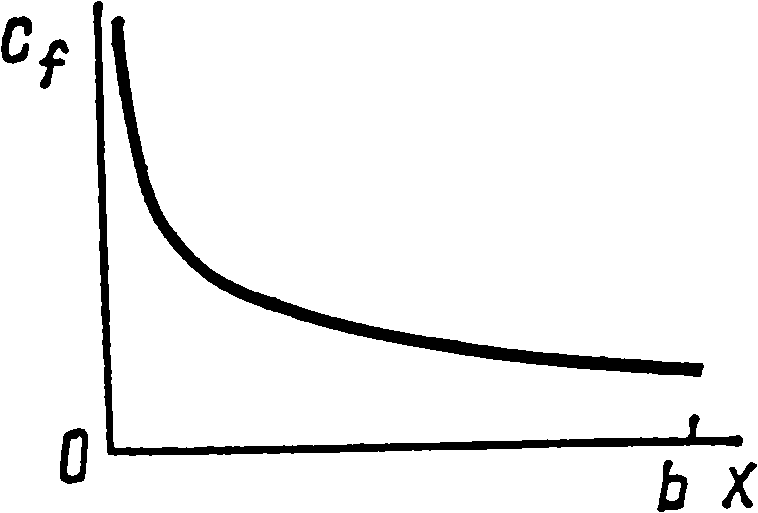
\includegraphics[width=0.25\linewidth]{img/plate-friction-coefficient-change}
		\caption{Изменение местного коэффициента трения вдоль пластинки.}
		\label{fig:12.8_plate-friction-coefficient-change}
	\end{figure}
	Из формулы следует, что местный коэффициент трения уменьшается при удалении от передней кромки (\cref{fig:12.8_plate-friction-coefficient-change}). Формула \eqref{eq:1228} дает хорошее совпадение с опытными данными, за исключением областей вблизи передней и задней кромок.\n
	Найдем силу трения. Обозначим $C_f$, коэффициент суммарного сопротивления трения, отнесенный к площади всей смоченной поверхности пластинки, т. е. $2lb$. Здесь $l$ --- длина пластинки вдоль ее размаха. Тогда
	\begin{gather*}
		X_\mathrm{тр} = C_f\frac{\rho v_\infty^2}{2}2lb = \int\limits_0^\delta\tau_0 2l\dd x.
	\end{gather*}
	Отсюда
	\begin{gather}\label{eq:1229}
		C_f = \frac{1}{b}\int\limits_0^\delta c_f\dd x.
	\end{gather}\n
	Подставляя в формулу \eqref{eq:1229} выражение $c_f$ \eqref{eq:1228}, получим
	\begin{gather}\label{eq:1230}
		C_f = \frac{1,3}{\sqrt{\Rey}}.
	\end{gather}\n
	Таким образом, коэффициент сопротивления трения плоской пластинки при ламинарном пограничном слое зависит от числа $\Rey$ и изменяется обратно пропорционально $\sqrt{\Rey}$.
	
	\subsubsection{Расчет турбулентного пограничного слоя на плоской пластинке}
	Законы турбулентного течения наиболее полно изучены для движения жидкости в круглых трубах. Используем результаты этих экспериментальных исследований для расчета пограничного слоя. Введем основное допущение: примем, что в пограничном слое на пластинке распределение скорости по сечению такое, как и в круглой трубе.\n
	Необходимо иметь в виду, что полного совпадения этих законов быть не может, так как распределение скорости в трубе устанавливается под воздействием градиента давления $\frac{\dd p}{\dd x} \ne 0$, а при обтекании пластинки $\frac{\dd p}{\dd x} = 0$. Однако небольшая разница в распределении скорости по нормали к поверхности при расчете пограничного слоя с помощью интегрального соотношения не имеет особого значения.\n
	Вводя гипотезу о тождественности безразмерных законов распределений скорости по толщине пограничного слоя плоской пластинки и по радиусу круглой цилиндрической трубы, можно принять, что изменение скорости внутри пограничного слоя пластинки при турбулентном течении определяется зависимостью
	\begin{gather}\label{eq:1231}
		\frac{v_x}{v_\infty} = \left(\frac{y}{\delta}\right)^\frac{1}{7},
	\end{gather}
	называемой \textit{законом одной седьмой}. Это первое дополнительное уравнение к интегральному соотношению.\n
	Вторым дополнительным уравнением является зависимость между значением касательного напряжения $\tau_0$, толщиной пограничного слоя $\delta$ и скоростью $v_\infty$ набегающего потока. Эту зависимость примем такой же, как при турбулентном течении жидкости в трубе:
	\begin{gather}\label{eq:1232}
		\tau_0 = 0,0225\rho v_\infty^2\left(\frac{\nu}{v_\infty\delta}\right)^\frac{1}{4},
	\end{gather}
	установленной экспериментально.\n
	Вычислим входящие в соотношение \eqref{eq:1223} интегралы:
	\begin{gather*}
		\int\limits_0^\delta\rho v_x\dd y = \frac{7}{8}\rho v_\infty\delta, \quad
		\int\limits_0^\delta\rho v_x^2\dd y = \frac{7}{9}\rho v_\infty^2\delta.
	\end{gather*}
	Подставляя найденные значения интегралов и выражение \eqref{eq:1232} в соотношение \eqref{eq:1223}, имеем
	\begin{gather*}
		\frac{7}{72}\frac{\dd\delta}{\dd x} = 0,0225\left(\frac{\nu}{v_\infty\delta}\right)^\frac{1}{4}.
	\end{gather*}\n
	Интегрируя и определяя постоянную интегрирования из условия $x = 0$, $\delta = 0$, после простых преобразований имеем:
	\begin{gather}
		\delta = 0,37\left(\frac{\nu}{v_\infty}\right)^\frac{1}{5}x^\frac{4}{5};\label{eq:1233}\\
		\bar{\delta} = 0,37\frac{\bar{x}^\frac{4}{5}}{\sqrt[5]{\Rey}},\label{eq:1234}
	\end{gather}
	где $\bar{\delta} = \delta/b$, $\bar{x} = x/b$, $\Rey = v_\infty b/\nu$.\n
	Из полученных выражений следует, что толщина турбулентного пограничного слоя нарастает более интенсивно (пропорционально $x^{4/5}$), чем ламинарного (для которого $\delta \sim x^{1/2}$), и обратно пропорциональна $\sqrt[5]{\Rey}$. Поэтому при прочих равных условиях $\delta_\mathrm{т} \gg \delta_\mathrm{л}$. Это объясняется тем, что вследствие поперечного перемешивания частиц в турбулентном потоке тормозящее влияние стенки распространяется на большее от нее расстояние.\n
	Толщина вытеснения для турбулентного пограничного слоя с распределением скорости по нормали к поверхности по закону одной седьмой $\delta^* = \delta/8$, а толщина потери импульса $\delta^{**} = 7\delta/72$.\n
	Определим силу трения $X_\mathrm{тр}$. Используя выражение \eqref{eq:1232}, получаем формулу для определения напряжения трения:
	\begin{gather*}
		\tau_0 = 0,0289\frac{\rho v_\infty^2\left(\frac{\nu}{v_\infty}\right)^\frac{1}{5}}{\sqrt[5]{x}}
	\end{gather*}
	и местного коэффициента трения:
	\begin{gather}\label{eq:1235}
		c_f = \frac{0,0578}{\sqrt[5]{\Rey_x}}.
	\end{gather}\n
	Тогда суммарный коэффициент сопротивления трения \eqref{eq:1229}
	\begin{gather}\label{eq:1236}
		C_f = \frac{0,072}{\sqrt[5]{\Rey}}.
	\end{gather}\n
	\begin{figure}[htbp]
		\centering
		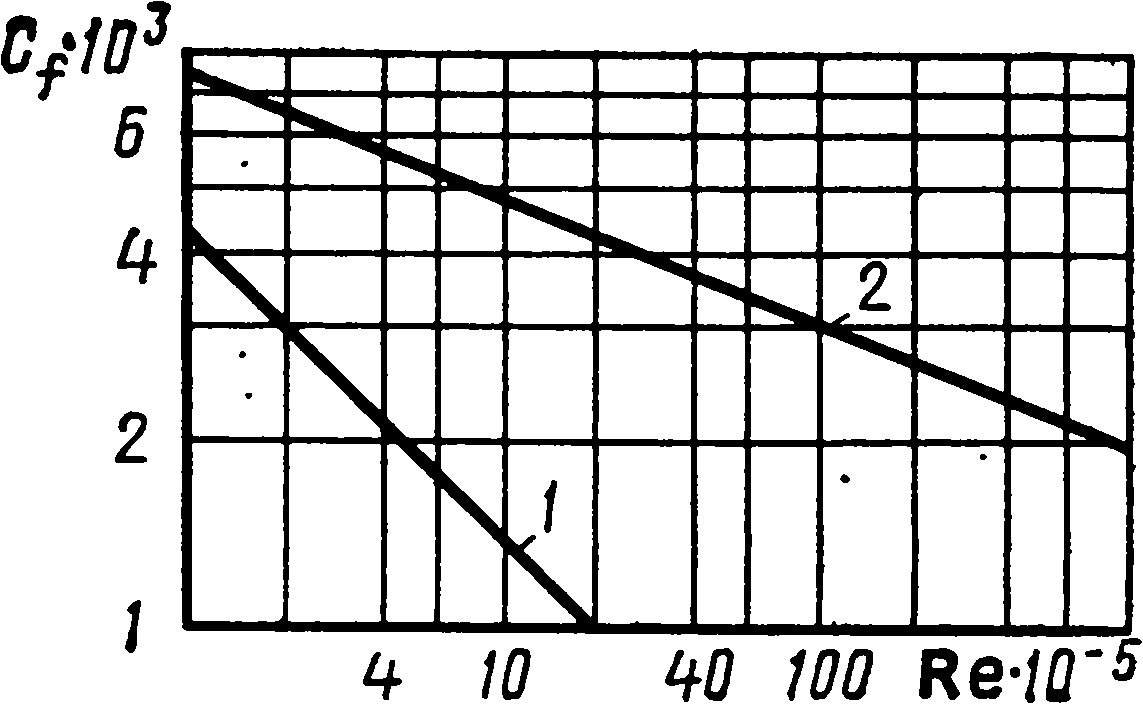
\includegraphics[width=0.35\linewidth]{img/plate-Cf-vs-Re}
		\caption{Зависимость коэффициента сопротивления трения пластинки от числа $\Rey$:\\\small{\textit{1} --- ламинарный пограничный слой; \textit{2} --- турбулентный пограничный слой.}}
		\label{fig:12.9_plate-cf-vs-re}
	\end{figure}
	Зависимость коэффициентов сопротивления трения от числа $\Rey$ удобно изображать в логарифмических координатах, за которые принимают $\lg\Rey$ и $\lg C_f$ (\cref{fig:12.9_plate-cf-vs-re}). При этом зависимость $C_f$ для ламинарного пограничного слоя изображается прямой \textit{1}, т. е. $\lg C_f = \lg 1,3 - 0,5\lg\Rey$ с угловым коэффициентом --- 0,5, а зависимость $C_f$ для турбулентного пограничного слоя --- прямой \textit{2}, т. е. $\lg C_f = \lg 0,072 - \left(1/5\right)\lg\Rey$ с угловым коэффициентом --- 1/5.\n
	Как видим, в обоих случаях с увеличением числа $\Rey$ коэффициент сопротивления трения убывает, но при турбулентном слое значительно медленнее, чем при ламинарном.\n
	Как показывают опыты, более точно коэффициент сопротивления трения пластинки в случае турбулентного пограничного слоя выражается формулой
	\begin{gather}\label{eq:1237}
		C_f = \frac{0,074}{\sqrt[5]{\Rey}}.
	\end{gather}\n
	Формула \eqref{eq:1237}, полученная из \eqref{eq:1236} только заменой в ней числового множителя 0,072 на 0,074, дает хорошее совпадение с результатами измерений, что свидетельствует в пользу принятого допущения о совпадении законов турбулентного течения в трубах и в пограничном слое пластинки.
	
	\subsubsection{Расчет смешанного пограничного слоя на плоской пластинке}
	\begin{figure}[htbp]
		\centering
		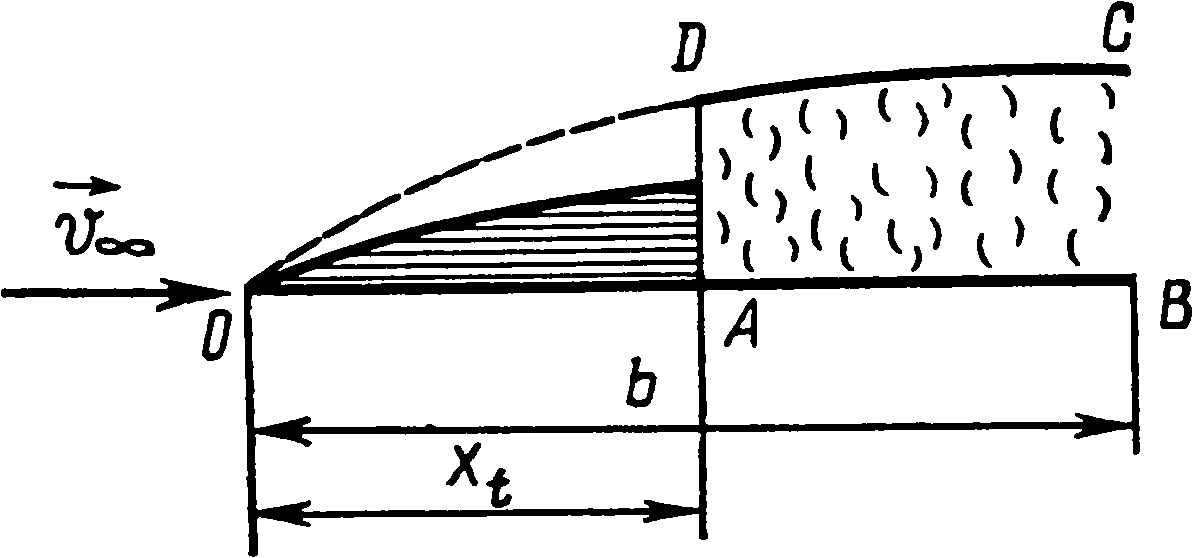
\includegraphics[width=0.35\linewidth]{img/flat-plate-mixed-boundary-layer}
		\caption{Схема для расчета смешанного пограничного слоя на плоской пластинке.}
		\label{fig:12.10_flat-plate-mixed-boundary-layer}
	\end{figure}
	Формула \eqref{eq:1237} справедлива, как уже известно, при условии, что пограничный слой на пластинке полностью турбулентен. Однако в действительности пограничный слой вблизи передней кромки остается ламинарным и становится турбулентным только на некотором расстоянии от передней кромки. Такой слой принято называть \textit{смешанным}. Очевидно, что наличие ламинарного слоя уменьшает сопротивление трения. Для определения сопротивления трения в случае смешанного пограничного слоя предположим, что:
	\begin{enumerate}
		\item переход от ламинарного пограничного слоя к турбулентному происходит мгновенно в точке $A$, называемой \textit{точкой перехода} (\cref{fig:12.10_flat-plate-mixed-boundary-layer}); $x_t$ --- координата точки перехода;
		\item изменение толщины турбулентного слоя и распределение скоростей и касательных напряжений в нем аналогичны тем, которые были бы, если бы турбулентный слой начинался не от точки $A$, а от передней кромки $O$.
	\end{enumerate}\n
	Исходя из этих предположений, расчет силы сопротивления трения можно произвести следующим образом. Обозначим $X_\mathrm{тр}''$ силу трения всей пластинки в предположении, что пограничный слой на всем ее протяжении турбулентный. Тогда, чтобы получить силу трения $X_\mathrm{тр}$ для смешанного слоя, нужно из $X_\mathrm{тр}''$ вычесть силу турбулентного трения переднего участка $OA$, т. е. $X_{\mathrm{тр}\;OA}''$, и прибавить к полученной разности силу трения этого же участка $OA$, считая его ламинарным, т. е. $X_{\mathrm{тр}\;OA}'$:
	\begin{gather*}
		X_\mathrm{тр} = X_\mathrm{тр}'' - X_{\mathrm{тр}\;OA}'' + X_{\mathrm{тр}\;OA}'.
	\end{gather*}\n
	Сила сопротивления трения переднего участка пластинки при ламинарном пограничном слое $C_{f\mathrm{л}}'\frac{\rho v_\infty^2}{2}2x_tl$, а при турбулентном $C_{f\mathrm{т}}'\frac{\rho v_\infty^2}{2}2x_tl$.\n
	Представим разность сопротивлений $\Delta X_\mathrm{тр}$ в следующем виде:
	\begin{gather*}
		\Delta X_\mathrm{тр} = X_{\mathrm{тр}\;OA}'' - X_{\mathrm{тр}\;OA}' = \frac{\rho v_\infty^2}{2}\left(C_{f\mathrm{т}}' - C_{f\mathrm{л}}'\right)2x_tl.
	\end{gather*}\n
	Тогда изменение коэффициента сопротивления трения пластинки в зависимости от протяженности ламинарного участка выразится в виде $\Delta C_f = \left(C_{f\mathrm{т}}' - C_{f\mathrm{л}}'\right)\bar{x}_t$, где $C_{f\mathrm{т}}'$, $C_{f\mathrm{л}}'$ --- коэффициенты сопротивления трения при полностью турбулентном и ламинарном пограничных слоях, определяемые по числу $\Rey_\mathrm{кр} = v_\infty x_t/\nu$, а $\bar{x}_t = x_t/b$ --- относительная координата точки перехода.\n
	Суммарный коэффициент сопротивления трения
	\begin{gather}\label{eq:1238}
		C_f = C_{f\mathrm{т}} - \Delta C_f.
	\end{gather}\n
	\begin{figure}[htbp]
		\centering
		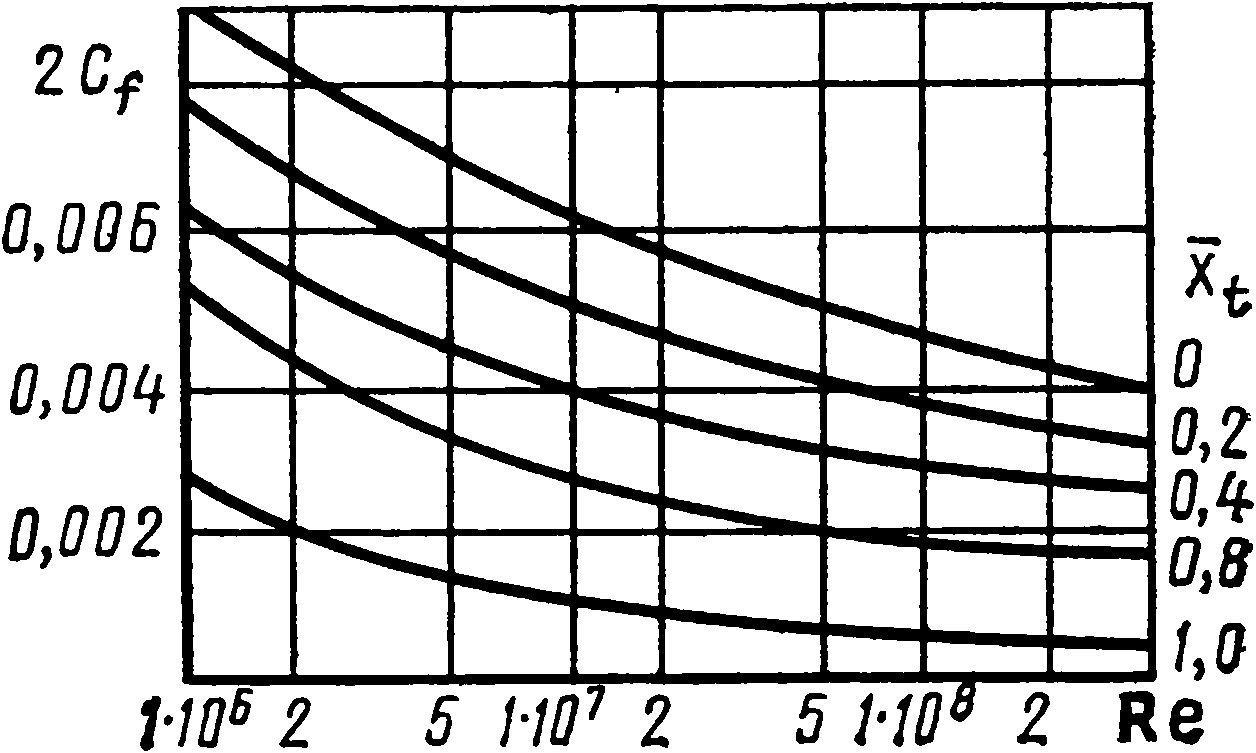
\includegraphics[width=0.35\linewidth]{img/2Cf-vs-Re-and-xt}
		\caption{Зависимости коэффициента сопротивления трения $2C_f$ от числа $\Rey$ и относительной координаты точки перехода при $\M = 0$.}
		\label{fig:12.11_2cf-vs-re-and-xt}
	\end{figure}
	Из изложенного следует, что \textit{сопротивление трения пластинки тем меньше, чем больше длина ламинарного участка пограничного слоя}. Следовательно, в случае смешанного пограничного слоя $C_f\left(\Rey,\; \bar{x}_t\right)$. На \cref{fig:12.11_2cf-vs-re-and-xt} приведены кривые зависимости коэффициента $2C_f$ от числа $\Rey$ и относительной координаты $\bar{x}_t$. Положение точки перехода обычно характеризуется числом $\Rey_\mathrm{кр} = v_\infty x_t/\nu$, называемым \textit{критическим числом Рейнольдса}. Значение $\Rey_\mathrm{кр}$ зависит от ряда факторов, основными из которых являются число $\Rey$, степень шероховатости поверхности, продольный градиент давления (т. е. форма тела), число $\M$, температура стенки. Кроме того, $\Rey_\mathrm{кр}$ зависит от степени турбулентности набегающего потока.\n
	При определении величины $\Rey_\mathrm{кр}$ в основном используют экспериментальные данные. Очевидно, что при увеличении $\Rey$, степени шероховатости поверхности, степени турбулентности набегающего потока точка перехода смещается вперед. При увеличении числа $\M$ число $\Rey_\mathrm{кр}$ уменьшается, а охлаждение поверхности способствует стабилизации ламинарного пограничного слоя, т. е. приводит к росту $\Rey_\mathrm{кр}$.\n
	При обтекании криволинейной поверхности наличие градиента давления $\left(\frac{\dd p}{\dd x} \ne 0\right)$ приводит к смещению точки перехода по сравнению с пластинкой, а именно: отрицательный градиент давления способствует стабилизации ламинарного пограничного слоя, т. е. смещению точки перехода назад, а положительный градиент давления приводит к смещению точки перехода вперед. На этом основано проектирование ламинаризированных крыловых профилей, которые, обладая увеличенной зоной ламинарного пограничного слоя, дают выигрыш в сопротивлении трения.
	
	\subsection{Пограничный слой при наличии продольного градиента давления. Отрыв потока}
	\begin{figure}[htbp]
		\centering
		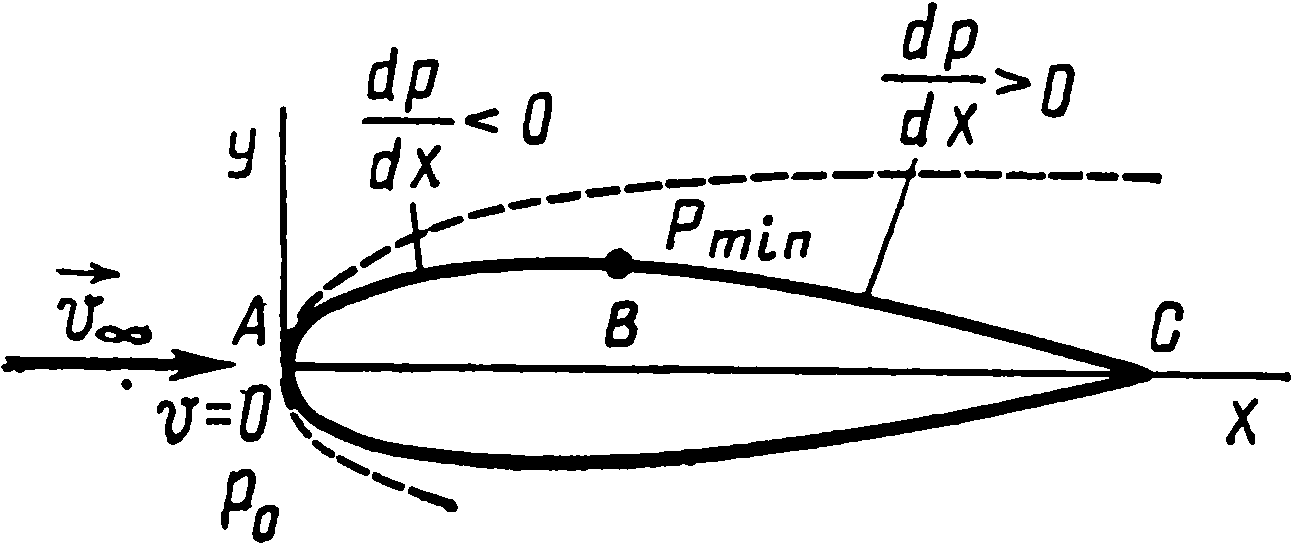
\includegraphics[width=0.35\linewidth]{img/profile-longitudinal-pressure-gradient}
		\caption{Продольный градиент давления на профиле.}
		\label{fig:12.15_profile-longitudinal-pressure-gradient}
	\end{figure}
	Рассмотрим обтекание криволинейной поверхности, например профиля крыла, дозвуковым потоком (\cref{fig:12.15_profile-longitudinal-pressure-gradient}). При этом на внешней границе пограничного слоя скорость $u$ --- величина переменная, зависящая от координаты $x$. Давление в пограничном слое криволинейной поверхности также функция $x$. Так как на поверхности профиля скорость сначала возрастает от точки $A$ до точки $B$, а затем убывает, то давление сначала уменьшается, а затем возрастает. Следовательно, частицы газа в пограничном слое около криволинейной поверхности движутся при наличии градиента давления $\frac{\dd p}{\dd x}$, как отрицательного, так и положительного по знаку. Этот факт существенно отличает пограничный слой около криволинейной поверхности от пограничного слоя вдоль плоской пластинки, где $\frac{\dd p}{\dd x} = 0$.\n
	Частицы невязкого (идеального) газа преодолевают при своем движении только силы давления --- на участке $AB$ под действием отрицательного градиента давления $\left(\frac{\dd p}{\dd x} < 0\right)$ частицы ускоряются, а в кормовой части $BC$ под действием положительного градиента давления $\frac{\dd p}{\dd x} > 0$ скорость уменьшается.\n
	\begin{figure}[htbp]
		\centering
		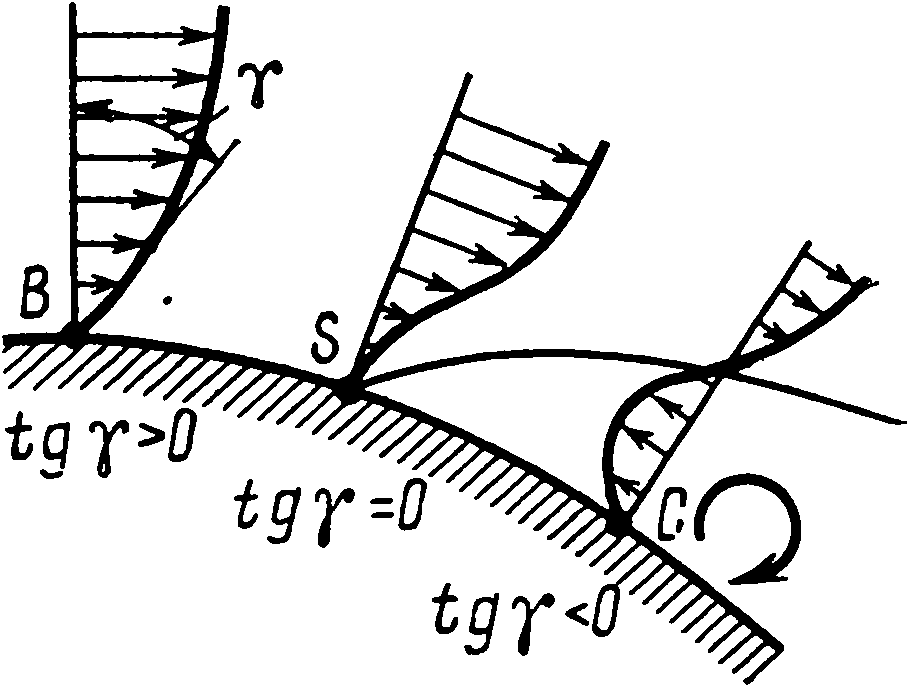
\includegraphics[width=0.3\linewidth]{img/normal-velocity-distribution}
		\caption{Распределение скорости по нормали к поверхности в различных сечениях пограничного слоя.}
		\label{fig:12.16_normal-velocity-distribution}
	\end{figure}
	В пограничном слое давление мало отличается от давления во внешнем потоке. Однако в непосредственной близости от поверхности тела из-за влияния вязкости скорость, а следовательно, и кинетическая энергия частиц малы (\cref{fig:12.16_normal-velocity-distribution}, сечение $B$).\n
	В кормовой части тела кинетической энергии частиц вблизи поверхности может оказаться недостаточно для преодоления положительного градиента давления. В этих условиях торможение приводит к остановке частиц, а затем под действием положительного градиента давления в пограничном слое возникает движение частиц, направленное в сторону, обратную основному потоку (\cref{fig:12.16_normal-velocity-distribution}, сечение $C$). Столкновение основного потока с противотоком приводит к оттеснению линий тока от поверхности и к отрыву пограничного слоя. При этом масса газа, движущегося в пограничном слое против направления основного потока, образует вихрь. Поэтому отрыв потока сопровождается всегда вихрями, которые периодически сходят с поверхности тела. Причиной отрыва потока являются вязкость и положительный градиент давления.\n
	Точка $S$, в которой $\left(\frac{\pp v_x}{\pp y}\right)_{y=0} = 0$, называется \textit{точкой отрыва потока}. Положение точки отрыва зависит прежде всего от значения положительного градиента давления. Для тел, имеющих малую кривизну поверхности и обтекаемых под малым углом атаки, градиент давления $\frac{\dd p}{\dd x}$ мал; практически можно считать, что отрыв потока отсутствует. При увеличении угла атаки градиент $\frac{\dd p}{\dd x}$ на верхней поверхности возрастает, что вызывает отрыв потока. Чем больше угол атаки, тем ближе точка отрыва к передней кромке.\n
	Отрыв потока и образование вихрей приводят к существенному изменению распределения давления в кормовой части тела по сравнению с безотрывным обтеканием. При этом распределение давления, рассчитанное для невязкого газа, не совпадает с действительным распределением давления. В кормовой части при обтекании тела с отрывом потока давление оказывается ниже, чем расчетное. Понижение давления в кормовой части приводит к появлению дополнительного сопротивления давления. Это сопротивление называют \textit{вихревым сопротивлением}. Для тонких профилей, крыльев и удлиненных тел вращения при малых углах атаки коэффициент этого сопротивления $c_{x\; \mathrm{а. вихр}}$ мал, а с увеличением угла атаки он возрастает.\n
	\begin{figure}[htbp]
		\centering
		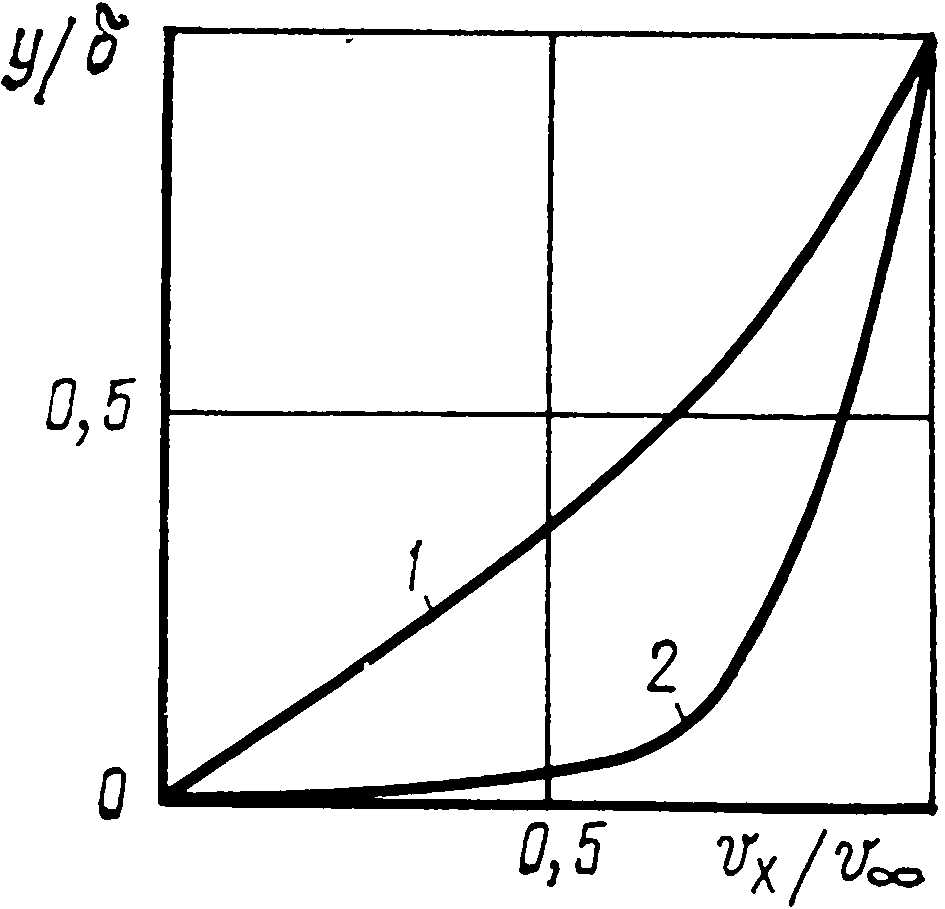
\includegraphics[width=0.3\linewidth]{img/boundary-layer-velocity-distribution}
		\caption{Распределение скорости по сечению ламинарного \textit{1} и турбулентного \textit{2} пограничных слоев.}
		\label{fig:12.17_boundary-layer-velocity-distribution}
	\end{figure}
	Отрыв пограничного слоя зависит также от режима течения газа. В случае турбулентного пограничного слоя отрыв потока затягивается, так как скорость частиц газа вблизи стенки в турбулентном пограничном слое оказывается больше, чем в ламинарном слое. Это наглядно видно из \cref{fig:12.17_boundary-layer-velocity-distribution}, на котором приведено сравнение распределения скорости по сечениям ламинарного и турбулентного слоев. Поэтому турбулентный пограничный слой может более успешно противостоять большим градиентам давления. В результате точка отрыва смещается вниз по потоку, вихревая зона за телом сужается. Это приводит к уменьшению вихревого сопротивления. Несмотря на некоторое увеличение сопротивления трения, полное сопротивление при этом часто оказывается меньше, чем в случае ламинарного пограничного слоя. Особенно наглядно это проявляется при обтекании таких тел, как цилиндр, сфера, у которых основным является сопротивление давления. Коэффициент сопротивления таких тел существенно зависит от числа $\Rey$. При малых числах $\Rey$ коэффициент $c_{x\mathrm{a}}$ значительно выше, чем при больших числах $\Rey$. Резкое уменьшение коэффициента $c_{x\mathrm{a}}$ происходит одновременно с переходом ламинарного пограничного слоя в турбулентный. Это объясняется тем, что при больших числах $\Rey$ вследствие перехода ламинарного пограничного слоя в турбулентный точка отрыва смещается назад, вихревая зона сужается, что приводит к резкому уменьшению коэффициента вихревого сопротивления.\n
	\begin{figure}[htbp]
		\centering
		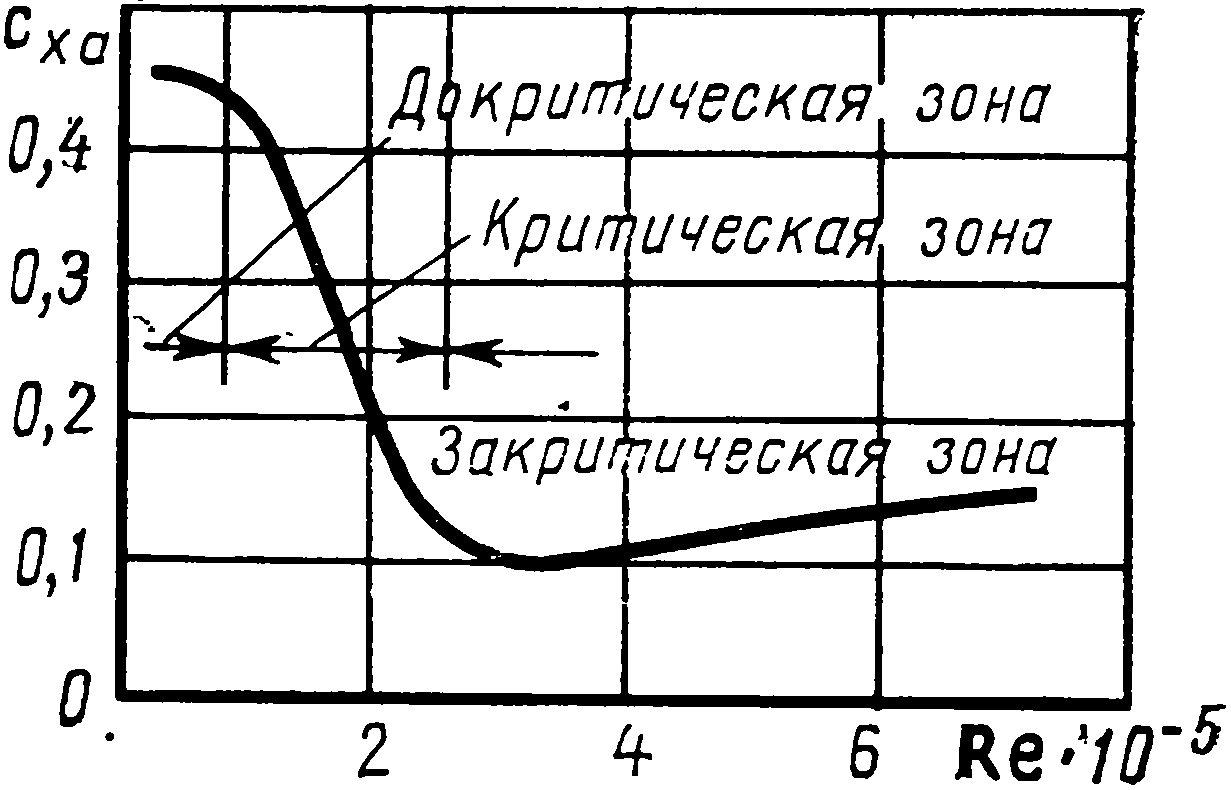
\includegraphics[width=0.35\linewidth]{img/cxa-vs-Re}
		\caption{Зависимость коэффициента сопротивления сферы $c_{x\mathrm{a}}$ от числа $\Rey$.}
		\label{fig:12.18_cxa-vs-re}
	\end{figure}
	На \cref{fig:12.18_cxa-vs-re} приведена зависимость коэффициента $c_{x\mathrm{a}}$ от числа $\Rey$ для сферы. Явление резкого уменьшения коэффициента сопротивления неудобообтекаемых тел называется \textit{кризисом сопротивления}.\n
	При больших скоростях наблюдается утолщение, а иногда и отрыв пограничного слоя вследствие взаимодействия скачка уплотнения с пограничным слоем. Скачок уплотнения при наличии пограничного слоя начинается не у поверхности, а на некотором расстоянии от нее --- на границе сверхзвукового участка пограничного слоя. При этом повышенное давление из области за скачком уплотнения по дозвуковому участку пограничного слоя вблизи поверхности распространяется вперед, в область перед скачком уплотнения. Это вызывает утолщение пограничного слоя, а при достаточном положительном перепаде давления может привести и к отрыву потока перед скачком уплотнения. В результате изменяются также форма и интенсивность скачка уплотнения.\n
	\begin{figure}[htbp]
		\centering
		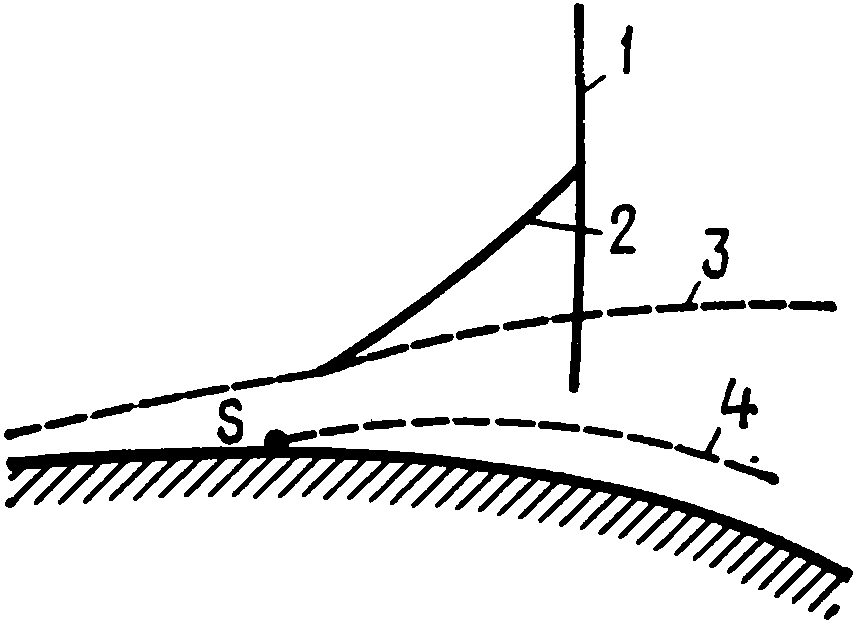
\includegraphics[width=0.35\linewidth]{img/compression-shock-boundary-layer-interaction}
		\caption{Взаимодействие скачка уплотнения с пограничным слоем при $\M_\mathrm{кр} < \M_\infty < 1$:\\\small{\textit{1} --- основной скачок уплотнения; \textit{2} --- дополнительный скачок уплотнения; \textit{3} --- граница пограничного слоя; \textit{4} --- граница зоны отрыва; $S$ --- точка отрыва потока.}}
		\label{fig:12.19_compression-shock-boundary-layer-interaction}
	\end{figure}
	Типичным примером такого обтекания является обтекание тел околозвуковым потоком $\left(\M_\mathrm{кр} < \M_\infty < 1\right)$. В этом случае повышенное давление за скачком уплотнения, замыкающим местную сверхзвуковую зону, распространяясь вперед через дозвуковую часть пограничного слоя, может вызвать отрыв потока и в соответствии с этим искривление линий тока во внешним потоке перед скачком уплотнения. В результате перед основным скачком уплотнения, близким к прямому, может возникнуть дополнительный косой скачок, образуя в совокупности $\lambda$-образный скачок уплотнения (\cref{fig:12.19_compression-shock-boundary-layer-interaction}).\n
	\begin{figure}[htbp]
		\centering
		\begin{minipage}{0.49\textwidth}
			\centering
			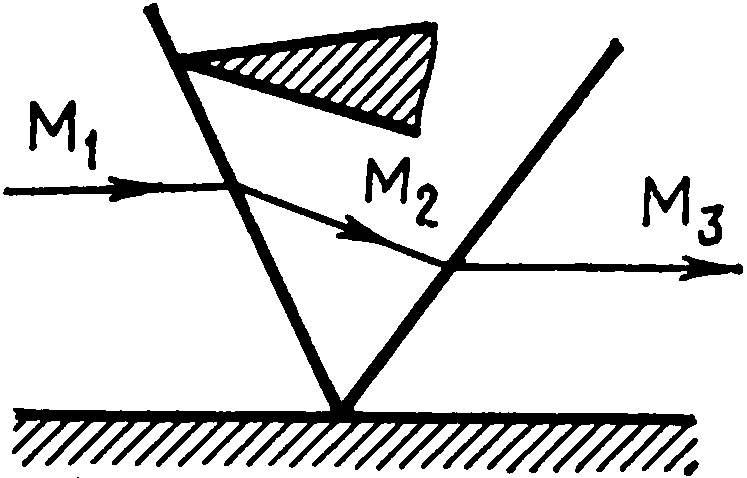
\includegraphics[width=0.5\textwidth]{img/falling-compression-shock-reflection}
			\captionof{figure}{Отражение падающего скачка уплотнения в невязком газе.}
			\label{fig:12.20_falling-compression-shock-reflection}
		\end{minipage}
		\hfill
		\begin{minipage}{0.49\textwidth}
			\centering
			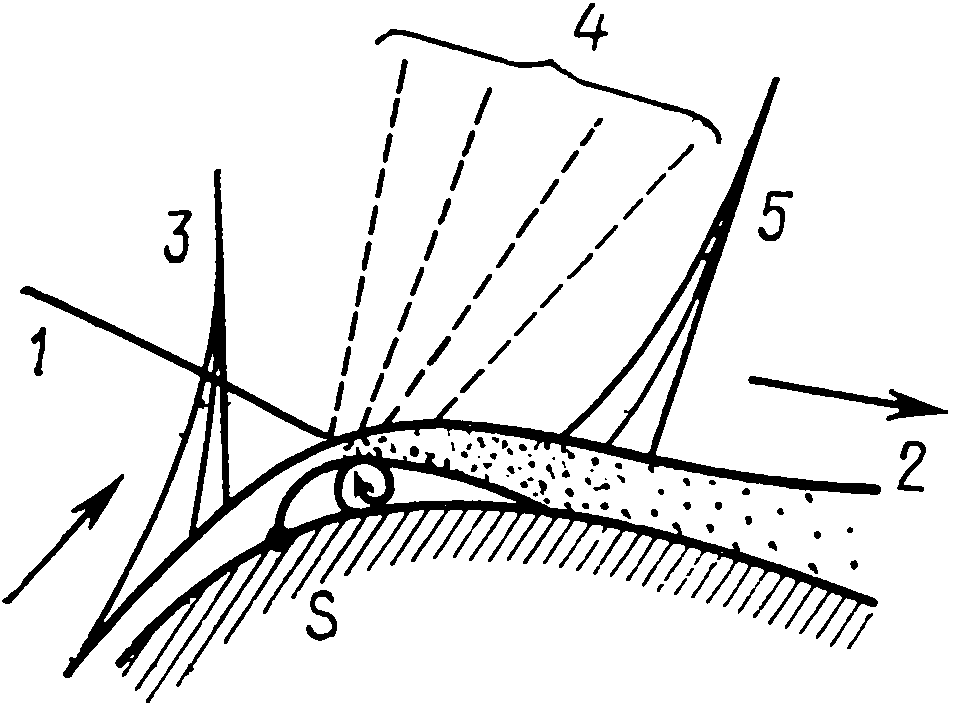
\includegraphics[width=0.75\textwidth]{img/falling-compression-shock-boundary-layer-interaction}
			\captionof{figure}{Взаимодействие падающего скачка уплотнения с пограничным слоем:\\\small{\textit{1} --- падающий скачок уплотнения; \textit{2} --- граница пограничного слоя; \textit{3} --- отраженный скачок уплотнения; \textit{4} --- область течения разрежения; \textit{5} --- скачки уплотнения; $S$ --- точка отрыва пограничного слоя.}}
			\label{fig:12.21_falling-compression-shock-boundary-layer-interaction}
		\end{minipage}
	\end{figure}
	Отрыв потока возникает также при наличии падающего скачка уплотнения. Плоский скачок, падающий на твердую поверхность, в невязком газе отражается от нее также в виде плоского скачка уплотнения $\left(\M_1 > \M_2 > \M_3\right)$ (\cref{fig:12.20_falling-compression-shock-reflection}). Наличие пограничного слоя существенно осложняет характер обтекания, так как при этом падающий скачок уплотнения при достаточном градиенте давления может вызвать отрыв пограничного слоя. Схематично характер обтекания поверхности с учетом взаимодействия падающего скачка уплотнения с пограничным слоем представлен на \cref{fig:12.21_falling-compression-shock-boundary-layer-interaction}.\n
	\begin{figure}[htbp]
		\centering
		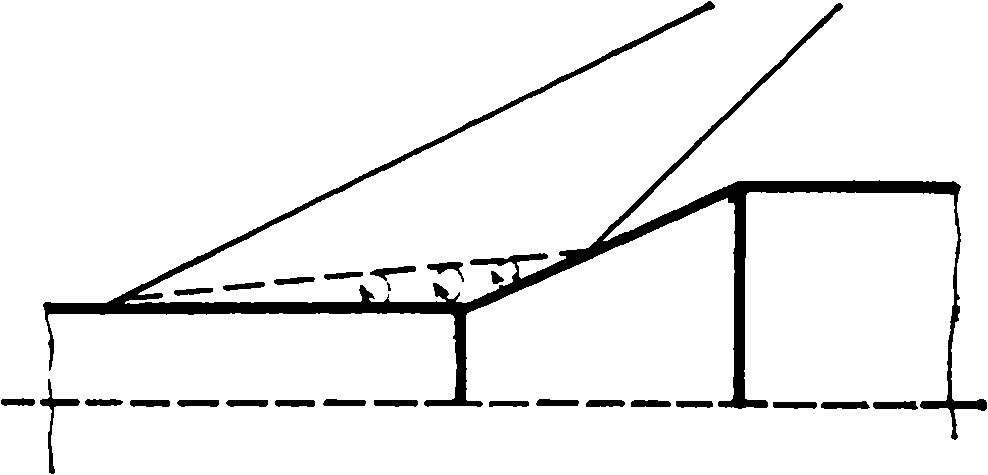
\includegraphics[width=0.35\linewidth]{img/stepped-body-boundary-layer-separation}
		\caption{Отрыв пограничного слоя на ступенчатом корпусе при $\M_\infty > 1$.}
		\label{fig:12.22_stepped-body-boundary-layer-separation}
	\end{figure}
	Отрыв потока вследствие подобного взаимодействия скачка уплотнения с пограничным слоем может произойти и при обтекании ступенчатого тела вблизи точки излома образующей (\cref{fig:12.22_stepped-body-boundary-layer-separation}).\n
	Экспериментальные исследования показывают, что отрыв потока существенно зависит от интенсивности скачка уплотнения и состояния пограничного слоя. Взаимодействие скачка уплотнения с пограничным слоем наиболее интенсивно проявляется в случае ламинарного пограничного слоя, который по сравнению с турбулентным слоем слабо сопротивляется тормозящему влиянию положительного градиента давления.
	
	\newpage
	\phantomsection
	\addcontentsline{toc}{section}{Список литературы}
	\begin{thebibliography}{99}
		\bibitem{1} Колесников Г.А. Аэродинамика летательных аппаратов : учебник для вузов по специальности «Самолетостроение» / Г.А. Колесников, В.К. Марков, А.А. Михайлюк [и др.] ; под редакцией Г.А. Колесникова. --- Москва : Машиностроение, 1993. --- 544 с. : ил.
		
		\bibitem{2} Аржаников Н.С. Аэродинамика летательных аппаратов : учебник для студентов авиационных специальностей вузов / Н.С. Аржаников, Г.С. Садекова. --- Москва : Высшая школа, 1983. --- 359 с. : ил.
		
		\bibitem{3} Кудрявцев Л.Д. Курс математического анализа : в 3 т. / Л.Д. Кудрявцев. --- Москва : Дрофа, 2003–2006. --- 3 т. --- (Высшее образование). --- ISBN 5-7107-5004-2.
		
		\bibitem{4} Фабрикант Н.Я. Аэродинамика. Общий курс : [учебное руководство] / Н.Я. Фабрикант. --- Москва : Наука, 1964. --- 814 с. : ил.
		
		\bibitem{5} Лойцянский Л.Г. Механика жидкости и газа : учебник для вузов / Л.Г. Лойцянский. --- 7-е изд., испр. --- Москва : Дрофа, 2003. --- 840 с. : ил., табл. --- (Классики отечественной науки). --- ISBN 5-7107-6327-6.
	\end{thebibliography}
\end{document}